\documentclass{article}

  % packages
    % basic stuff for rendering math
    \usepackage[letterpaper, top=1in, bottom=1in, left=1in, right=1in]{geometry}
    \usepackage[utf8]{inputenc}
    \usepackage[english]{babel}
    \usepackage{amsmath} 
    \usepackage{amssymb}
    % \usepackage{amsthm}

    % extra math symbols and utilities
    \usepackage{mathtools}        % for extra stuff like \coloneqq
    \usepackage{mathrsfs}         % for extra stuff like \mathsrc{}
    \usepackage{centernot}        % for the centernot arrow 
    \usepackage{bm}               % for better boldsymbol/mathbf 
    \usepackage{enumitem}         % better control over enumerate, itemize
    \usepackage{hyperref}         % for hypertext linking
    \usepackage{fancyvrb}          % for better verbatim environments
    \usepackage{newverbs}         % for texttt{}
    \usepackage{xcolor}           % for colored text 
    \usepackage{listings}         % to include code
    \usepackage{lstautogobble}    % helper package for code
    \usepackage{parcolumns}       % for side by side columns for two column code
    

    % page layout
    \usepackage{fancyhdr}         % for headers and footers 
    \usepackage{lastpage}         % to include last page number in footer 
    \usepackage{parskip}          % for no indentation and space between paragraphs    
    \usepackage[T1]{fontenc}      % to include \textbackslash
    \usepackage{footnote}
    \usepackage{etoolbox}

    % for custom environments
    \usepackage{tcolorbox}        % for better colored boxes in custom environments
    \tcbuselibrary{breakable}     % to allow tcolorboxes to break across pages

    % figures
    \usepackage{pgfplots}
    \pgfplotsset{compat=1.18}
    \usepackage{float}            % for [H] figure placement
    \usepackage{tikz}
    \usepackage{tikz-cd}
    \usepackage{circuitikz}
    \usetikzlibrary{arrows}
    \usetikzlibrary{arrows.meta}
    \usetikzlibrary{positioning}
    \usetikzlibrary{patterns}
    \usetikzlibrary{calc}
    \usepackage{graphicx}
    \usepackage{algorithmic}
    \usepackage{caption} 
    \usepackage{subcaption}
    \captionsetup{font=small}

    % for tabular stuff 
    \usepackage{dcolumn}

    \usepackage[nottoc]{tocbibind}
    \pdfsuppresswarningpagegroup=1
    \hfuzz=5.002pt                % ignore overfull hbox badness warnings below this limit

  % New and replaced operators
    \DeclareMathOperator{\Tr}{Tr}
    \DeclareMathOperator{\Sym}{Sym}
    \DeclareMathOperator{\Span}{span}
    \DeclareMathOperator{\im}{Im}
    \DeclareMathOperator{\Div}{div}
    \DeclareMathOperator{\curl}{curl}
    \DeclareMathOperator{\GL}{GL}
    \DeclareMathOperator{\SL}{SL}
    \DeclareMathOperator{\GA}{GA}
    \DeclareMathOperator{\std}{std}
    \DeclareMathOperator{\Cov}{Cov}
    \DeclareMathOperator{\Var}{Var}
    \DeclareMathOperator{\Corr}{Corr}
    \DeclareMathOperator{\Int}{Int}
    \DeclareMathOperator{\Id}{Id}
    \DeclareMathOperator{\Lie}{Lie}
    \DeclareMathOperator{\Hom}{Hom}
    \DeclareMathOperator{\Alt}{Alt}
    \DeclareMathOperator{\rank}{rank}
    \DeclareMathOperator{\conv}{conv}
    \DeclareMathOperator{\aff}{aff}
    \DeclareMathOperator{\arccot}{arccot}
    \newcommand{\ket}[1]{\ensuremath{\left|#1\right\rangle}}
    \newcommand{\bra}[1]{\ensuremath{\left\langle#1\right|}}
    \newcommand{\braket}[2]{\langle #1 | #2 \rangle}
    \newcommand{\qed}{\hfill$\blacksquare$}     % I like QED squares to be black

  % Custom Environments
    \newtcolorbox[auto counter, number within=section]{question}[1][]
    {
      colframe = orange!25,
      colback  = orange!10,
      coltitle = orange!20!black,  
      breakable, 
      title = \textbf{Question \thetcbcounter ~(#1)}
    }

    \newtcolorbox[auto counter, number within=section]{exercise}[1][]
    {
      colframe = teal!25,
      colback  = teal!10,
      coltitle = teal!20!black,  
      breakable, 
      title = \textbf{Exercise \thetcbcounter ~(#1)}
    }
    \newtcolorbox[auto counter, number within=section]{solution}[1][]
    {
      colframe = violet!25,
      colback  = violet!10,
      coltitle = violet!20!black,  
      breakable, 
      title = \textbf{Solution \thetcbcounter}
    }
    \newtcolorbox[auto counter, number within=section]{lemma}[1][]
    {
      colframe = red!25,
      colback  = red!10,
      coltitle = red!20!black,  
      breakable, 
      title = \textbf{Lemma \thetcbcounter ~(#1)}
    }
    \newtcolorbox[auto counter, number within=section]{theorem}[1][]
    {
      colframe = red!25,
      colback  = red!10,
      coltitle = red!20!black,  
      breakable, 
      title = \textbf{Theorem \thetcbcounter ~(#1)}
    } 
    \newtcolorbox[auto counter, number within=section]{proposition}[1][]
    {
      colframe = red!25,
      colback  = red!10,
      coltitle = red!20!black,  
      breakable, 
      title = \textbf{Proposition \thetcbcounter ~(#1)}
    } 
    \newtcolorbox[auto counter, number within=section]{corollary}[1][]
    {
      colframe = red!25,
      colback  = red!10,
      coltitle = red!20!black,  
      breakable, 
      title = \textbf{Corollary \thetcbcounter ~(#1)}
    } 
    \newtcolorbox[auto counter, number within=section]{proof}[1][]
    {
      colframe = orange!25,
      colback  = orange!10,
      coltitle = orange!20!black,  
      breakable, 
      title = \textbf{Proof. }
    } 
    \newtcolorbox[auto counter, number within=section]{definition}[1][]
    {
      colframe = yellow!25,
      colback  = yellow!10,
      coltitle = yellow!20!black,  
      breakable, 
      title = \textbf{Definition \thetcbcounter ~(#1)}
    } 
    \newtcolorbox[auto counter, number within=section]{example}[1][]
    {
      colframe = blue!25,
      colback  = blue!10,
      coltitle = blue!20!black,  
      breakable, 
      title = \textbf{Example \thetcbcounter ~(#1)}
    } 
    \newtcolorbox[auto counter, number within=section]{code}[1][]
    {
      colframe = green!25,
      colback  = green!10,
      coltitle = green!20!black,  
      breakable, 
      title = \textbf{Code \thetcbcounter ~(#1)}
    } 
    \newtcolorbox[auto counter, number within=section]{algo}[1][]
    {
      colframe = green!25,
      colback  = green!10,
      coltitle = green!20!black,  
      breakable, 
      title = \textbf{Algorithm \thetcbcounter ~(#1)}
    } 

    \BeforeBeginEnvironment{example}{\savenotes}
    \AfterEndEnvironment{example}{\spewnotes}
    \BeforeBeginEnvironment{lemma}{\savenotes}
    \AfterEndEnvironment{lemma}{\spewnotes}
    \BeforeBeginEnvironment{theorem}{\savenotes}
    \AfterEndEnvironment{theorem}{\spewnotes}
    \BeforeBeginEnvironment{corollary}{\savenotes}
    \AfterEndEnvironment{corollary}{\spewnotes}
    \BeforeBeginEnvironment{proposition}{\savenotes}
    \AfterEndEnvironment{proposition}{\spewnotes}
    \BeforeBeginEnvironment{definition}{\savenotes}
    \AfterEndEnvironment{definition}{\spewnotes}
    \BeforeBeginEnvironment{exercise}{\savenotes}
    \AfterEndEnvironment{exercise}{\spewnotes}
    \BeforeBeginEnvironment{proof}{\savenotes}
    \AfterEndEnvironment{proof}{\spewnotes}
    \BeforeBeginEnvironment{solution}{\savenotes}
    \AfterEndEnvironment{solution}{\spewnotes}
    \BeforeBeginEnvironment{question}{\savenotes}
    \AfterEndEnvironment{question}{\spewnotes}
    \BeforeBeginEnvironment{code}{\savenotes}
    \AfterEndEnvironment{code}{\spewnotes}
    \BeforeBeginEnvironment{algo}{\savenotes}
    \AfterEndEnvironment{algo}{\spewnotes}

    \definecolor{dkgreen}{rgb}{0,0.6,0}
    \definecolor{gray}{rgb}{0.5,0.5,0.5}
    \definecolor{mauve}{rgb}{0.58,0,0.82}
    \definecolor{darkblue}{rgb}{0,0,139}
    \definecolor{lightgray}{gray}{0.93}
    \renewcommand{\algorithmiccomment}[1]{\hfill$\triangleright$\textcolor{blue}{#1}}

    % default options for listings (for code)
    \lstset{
      autogobble,
      frame=ltbr,
      language=Python,
      aboveskip=3mm,
      belowskip=3mm,
      showstringspaces=false,
      columns=fullflexible,
      keepspaces=true,
      basicstyle={\small\ttfamily},
      numbers=left,
      firstnumber=1,                        % start line number at 1
      numberstyle=\tiny\color{gray},
      keywordstyle=\color{blue},
      commentstyle=\color{dkgreen},
      stringstyle=\color{mauve},
      backgroundcolor=\color{lightgray}, 
      breaklines=true,                      % break lines
      breakatwhitespace=true,
      tabsize=3, 
      xleftmargin=2em, 
      framexleftmargin=1.5em, 
      stepnumber=1
    }

  % Page style
    \pagestyle{fancy}
    \fancyhead[L]{Linear Algebra}
    \fancyhead[C]{Muchang Bahng}
    \fancyhead[R]{Spring 2020} 
    \fancyfoot[C]{\thepage / \pageref{LastPage}}
    \renewcommand{\footrulewidth}{0.4pt}          % the footer line should be 0.4pt wide
    \renewcommand{\thispagestyle}[1]{}  % needed to include headers in title page

\begin{document}

\title{Linear Algebra}
\author{Muchang Bahng}
\date{Spring 2020}

\maketitle
\tableofcontents
\pagebreak

This covers computability theory, complexity theory, and automata theory. 
Alphabet. Boolean logic


\section{Vector Spaces}

  \begin{definition}[Vector Space]
     A \textbf{vector space over a field $F$} consists of an abelian group $(V, +)$ and an operation called \textbf{scalar multiplication} 
     \begin{equation}
       \cdot: F \times V \rightarrow V
     \end{equation}
    such that for all $x, y\in V$ and $\lambda, \mu \in F$, we have 
    \begin{enumerate}
      \item $\lambda \cdot (x + y) = \lambda \cdot x + \lambda \cdot y$
      \item $(\lambda + \mu) \cdot x = \lambda \cdot x + \mu \cdot x$ 
      \item $(\lambda \mu) \cdot x = \lambda \cdot (\mu \cdot x )$, which equals $(\mu \lambda) \cdot x = \mu \cdot (\lambda \cdot x)$ since $F$ is commutative 
      \item $1 \cdot x = x$ , where $1$ is the unity of $F$
    \end{enumerate}
  \end{definition}

  \begin{definition}
    A \textbf{left R-module} $M$ consists of an abelian group $(M, +)$ and an operation called \textbf{scalar multiplication}
    \begin{equation}
      \cdot: R \times M \longrightarrow M
    \end{equation}
    such that for all $\lambda, \mu \in R$ and $x, y \in M$, we have 
    \begin{enumerate}
      \item $\lambda \cdot (x + y) = \lambda \cdot x + \lambda \cdot y$
      \item $(\lambda + \mu) \cdot x = \lambda \cdot x + \mu \cdot x$ 
      \item $(\lambda \mu) \cdot x = \lambda \cdot (\mu \cdot x )$, not necessarily equaling $(\mu \lambda) \cdot x = \mu \cdot (\lambda \cdot x)$
      \item $1 \cdot x = x$ , where $1$ is the unity of $R$
    \end{enumerate}
    Note that a left $R$-module is a vector space if and only if $R$ is a field.
  \end{definition}

  \begin{definition}
    A \textbf{right $R$-module} $M$ is defined analogously to a left $R$-module, except that the scalar multiplication operation is defined
    \begin{equation}
      \cdot: M \times R \longrightarrow M
    \end{equation}
  \end{definition}

  \begin{definition}
    Let $A$ be a vector space over a field $F$ equipped with an additional binary operation 
    \begin{equation}
      \times: A \times A \longrightarrow A
    \end{equation}
    $A$ is an \textbf{algebra over $F$} if the following identities hold for all $x, y, z \in A$ and all $\lambda, \mu \in F$. 
    \begin{enumerate}
      \item Right distributivity. $(x + y) \times z = x \times z + y \times z$ 
      \item Left distributivity. $z \times (x + y) = z \times x + z \times y$
      \item Compatibility with scalars. $(\lambda \cdot x ) \times (\mu \cdot y) = (\lambda \mu) \cdot (x \times y)$ 
    \end{enumerate}
  \end{definition}

  Note that vector multiplication of an algebra does not need to be commutative. 

  \begin{example}
    The set of all $n \times n$ matrices with matrix multiplication is a noncommutative, associative algebra. Similarly, the set of all linear endomorphisms of a vector space $V$ with composition is a noncommutative, associative algebra. 
  \end{example}

  \begin{example}
    $\mathbb{R}^3$ equipped with the cross product is an algebra, where the cross product is \textbf{anticommutative}, that is $x \times y = - y \times x$. $\times$ is also nonassociative, but rather satisfies an alternative identity called the \textbf{Jacobi Identity}. 
  \end{example}

  \begin{example}
    The set of all polynomials defined on an interval $[a,b]$ is an infinite-dimensional subalgebra of the set of all functions $f: \mathbb{R} \longrightarrow \mathbb{R}$ defined on $[a,b]$.
  \end{example}

  \begin{definition}
    Similar to division rings, a \textbf{division algebra} is an algebra where the operation of "division" defined as such: Given any $a \in A$, nonzero $b \in A$, there exists solutions to the equation
    \begin{equation}
      A = bx
    \end{equation}
    that are unique. If we wish, we can distinguish left and right division to be the solutions of $A = b x$ and $A = x b$. 
  \end{definition}

  \begin{definition}
    Here are examples of division algebras.
    \begin{enumerate}
      \item $\mathbb{R}$ is a $1$-dimensional algebra over itself. 
      \item $\mathbb{C}$ is a $2$-dimensional algebra over $\mathbb{R}$. 
      \item There exists no $3$-dimensional algebra. 
      \item Quaternions forms a $4$-dimensional algebra over $\mathbb{R}$. 
    \end{enumerate}
  \end{definition}

  \begin{theorem}[Eigenvector Conditions for Algebraic Closedness]
    A field $F$ is algebraically closed if and only if for each natural number $n$, every endomorphism of $F^n$ (that is, ever linear map from $F^n$ to itself) has at least one eigenvector. 
  \end{theorem}
  \begin{proof}
    An endomorphism of $F^n$ has an eigenvector if and only if its characteristic polynomial has some root. $(\rightarrow)$ So, when $F$ is algebraically closed, every characteristic polynomial, which is an element of $F[x]$, must have a root. $(\leftarrow)$ Assume that every characteristic polynomial has some root, and let $p \in F[x]$. Dividing the polynomial by a scalar doesn't change its roots, so we can assume $p$ to have leading coefficient $1$. If $p(x) = a_0 + a_1 x + ... + x^n$, then we can identify matrix 
    \begin{equation}
      A = \begin{pmatrix}
      0 & 0 & ... & 0 & -a_0 \\
      1 & 0 & ... & 0 & -a_1 \\
      0 & 1 & ... & 0 & -a_2 \\
      ... & ... & ... & ... & ... \\
      0 & 0 & ... & 1 & -a_{n-1}
      \end{pmatrix}
    \end{equation}
    such that the characteristic polynomial of $A$ is $p$. 
  \end{proof}


\subsection{Modules}

  Vector space but over a ring. 

\subsection{Algebras}

  Vector space with bilinear product.  

\subsection{The Algebra of Quaternions}

  \begin{definition}
    The \textbf{quaternions} form an algebra of $4$-dimensional vectors over $\mathbb{R}$, with elements of the form
    \begin{equation}
      (a, b, c, d) \equiv a + bi + cj + dk
    \end{equation}
    where $a$ is called the \textbf{scalar portion} and $bi + cj + dk$ is called the \textbf{vector/imaginary portion}. The algebra of quaternions is denoted $\mathbb{H}$, which stands for "Hamilton." $\mathbb{H}$ is a $4$-dimensional associative normed division algebra over $\mathbb{R}$. 
  \end{definition}

  From looking at the multiplication table, we can see that multiplication in $\mathbb{H}$ is not commutative. 
  \begin{center}
    \begin{tabular}{|c|c|c|c|c|}
    \hline
    i & i & -1 & k & -j \\ 
    \hline
    j & j & -k & -1 & i \\ 
    \hline
    k & k & j & -i & -1 \\ 
    \hline
    \end{tabular}
  \end{center}
  Note the identity 
  \begin{equation}
    i^2 = j^2 = k^2 = -1
  \end{equation}
  The algebra of quaternions are in fact the first noncommutative algebra to be discovered! 

  \begin{theorem}
    $\mathbb{H}$ and $\mathbb{C}$ are the only finite-dimensional divisions rings containing $\mathbb{R}$ as a proper subring. 
  \end{theorem}

  \begin{definition}
    The \textbf{quaternion group}, denoted $Q_8$ is a nonabelian group of order $8$, isomorphic to a certain $8$-element subset in $\mathbb{H}$ under multiplication. It's group presentation is 
    \begin{equation}
      Q_8 = \big\langle \bar{e}, i, j, k \;|\; \bar{e}^2 = e, i^2 = j^2 = k^2 = ijk = \bar{e} \big\rangle
    \end{equation}
  \end{definition}

  Going back to the algebra, we can set $\{1, i, j, k\}$ as a basis and define addition and scalar multiplication component-wise, and multiplication (called the \textbf{Hamilton product}) with properties
  \begin{enumerate}
    \item The real quaternion $1$ is the identity element. 
    \item All real quaternions commute with quaternions: $a q = q a$ for all $a \in \mathbb{R}, q \in \mathbb{H}$. 
    \item Every quaternion has an inverse with respect to the Hamilton product. 
      \begin{equation}
        (a + bi + cj + dk)^{-1} = \frac{1}{a^2 + b^2 + c^2 + d^2} \big( a - bi - cj - dk\big)
      \end{equation}
  \end{enumerate}
  Note that property 3 allows $\mathbb{H}$ to be a division algebra. 

  \begin{theorem}[Scalar and Vector Components]
    Let the quaternion be divided up into a scalar and vector part with the bjective mapping $a + bi + cj + dk \mapsto \big(a, (b, c, d)\big)$. 
    \begin{equation}
      q = (r, v), r \in \mathbb{R}, v \in \mathbb{R}^3
    \end{equation}
    Then, the formulas for addition and multiplication are
    \begin{align*}
      q_1 + q_2 & = (r_1, v_1) + (r_2, v_2) = (r_1 + r_2, v_1 + v_2) \\
      q_1 \cdot q_2 & = (r_1, v_1) \cdot (r_2, v_2) = (r_1 r_2 - v_1 \cdot v_2, r_1 v_2 + r_2 v_1 + v_1 \times v_2)
    \end{align*}
    where the $\cdot$ and $\times$ on the right hand side represnts the dot product and cross product, respectively. 
  \end{theorem}

  \begin{definition}
    The conjugate of a quaternion $q = a + bi + cj + dk$ is defined 
    \begin{equation}
      \bar{q}, q^* \equiv a - bi - cj - dk
    \end{equation}
    It has properties
    \begin{enumerate}
      \item $q^{**} = q$
      \item $(q p)^* = p^* q^*$
    \end{enumerate}
    $q^*$ can also be expressed in terms of addition and multiplication. 
    \begin{equation}
      q^* = -\frac{1}{2} \big( q + iqi + jqj + kqk \big)
    \end{equation}
  \end{definition}

  \begin{definition}
    The \textbf{norm} of $q$ is defined
    \begin{equation}
      ||q|| \equiv \sqrt{q^* q} = \sqrt{q q^*} = \sqrt{a^2 + b^2 + c^2 + d^2}
    \end{equation}
    with properties
    \begin{enumerate}
      \item Scaling factor. $||\alpha q|| = |\alpha| ||q||$
      \item Multiplicative. $||p q|| = ||p|| ||q||$
    \end{enumerate}
  \end{definition}

  The norm allows us to define a metric 
  \begin{equation}
    d(p, q) \equiv ||p - q||
  \end{equation}
  This makes $\mathbb{H}$ a metric space, with addition and multiplication continuous on the metric topology. 

  \begin{definition}
    The \textbf{unit quaternion} is defined to be
    \begin{equation}
      U_q = \frac{q}{||q||}
    \end{equation}
  \end{definition}

  \begin{corollary}
    Every quaternion has a polar decomposition
    \begin{equation}
      q = U_q \cdot ||q||
    \end{equation}
    With this, we can redefine the inverse as
    \begin{equation}
      q^{-1} = \frac{q^*}{||q||^2}
    \end{equation}
  \end{corollary}

\subsubsection{Matrix Representations of Quaternions}

  We can represent $q$ with $2 \times 2$ matrices over $\mathbb{C}$ or $4\times 4 $ matrices over $\mathbb{R}$. 

  \begin{theorem}
    The following representation is an injective homomorphism $\rho: \mathbb{H} \longrightarrow \GL(2, \mathbb{C})$. 
    \begin{equation}
      \rho: a + bi + cj + dk \mapsto \begin{pmatrix}
      a+bi & c+ di \\ -c + di & a - bi
      \end{pmatrix}
    \end{equation}
    It has properties
    \begin{enumerate}
      \item Constraining any two of $b, c, d$ to $0$ produces a representation of the complex numbers. When $c = d = 0$, this is called the \textbf{diagonal representation}. 
      \begin{align*}
        \begin{pmatrix}
        a+bi & 0 \\ 0 & a-bi
        \end{pmatrix},  \begin{pmatrix}
        a & c \\ -c & a
        \end{pmatrix},  \begin{pmatrix}
        a & di \\ di & a
        \end{pmatrix}
      \end{align*}
      \item The norm of a quaternion is the square root of the determinant of its corresponding matrix representation. 
        \begin{equation}
          ||q|| = \sqrt{\det \begin{pmatrix}
          a+bi & c+di \\ -c+di & a-bi
          \end{pmatrix}} = \sqrt{(a^2 + b^2) + (c^2 + d^2)}
        \end{equation}
      \item The conjugate of a quaternion corresponds to the conjugate (Hermitian) transpose of its matrix representation. 
        \begin{equation}
          \rho(q^*) = \rho(q)^H \iff a-bi-cj-dk \mapsto \begin{pmatrix}
          a-bi & -c-di \\ c-di & a+bi
          \end{pmatrix}
        \end{equation}
      \item The restriction of this representation to only unit quaternions leads to an isomorphism between the subgroup of unit quaternions and their corresponding image in SU$(2)$. Topologically, the unit quaternions is the $3$-sphere, so the underlying space SU$(2)$ is also a $3$-sphere. More specifically, 
        \begin{equation}
          \frac{\text{SU}(2)}{2} \simeq \text{SO}(3)
        \end{equation}
    \end{enumerate}
  \end{theorem}

  \begin{theorem}
  The following representation of $\mathbb{H}$ is an injective homomorphism $\rho: \mathbb{H} \longrightarrow \GL(4, \mathbb{R})$. 
  \begin{equation}
    \rho: a+bi+cj+dk \mapsto \begin{pmatrix}
    a&-b&-c&-d \\
    b&a&-d&c\\
    c&d&a&-b\\
    d&-c&b&a
    \end{pmatrix}
  \end{equation}
  or also as
  \begin{equation}
    a \begin{pmatrix}
    1 &0 &0 &0 \\
    0& 1&0&0\\
    0&0&1&0\\
    0&0&0&1
    \end{pmatrix} + b \begin{pmatrix}
    0&-1&0&0\\1&0&0&0\\0&0&0&-1\\0&0&1&0
    \end{pmatrix} + c\begin{pmatrix}
    0&0&-1&0\\0&0&0&1\\1&0&0&0\\0&-1&0&0
    \end{pmatrix} + d \begin{pmatrix}
    0&0&0&-1\\0&0&-1&0\\0&1&0&0\\1&0&0&0
    \end{pmatrix}
  \end{equation}
  It has properties
  \begin{enumerate}
    \item $\rho(q^*) = \rho(q)^T$
    \item The fourth power of the norm is the determinant of the matrix 
      \begin{equation}
        ||q||^4 = \det\big( \rho (q)\big)
      \end{equation}
    \item Similarly, with the $2\times 2$ representation, complex number representations can be produced by restricting $2$ of $b, c, d$ to $0$. 
  \end{enumerate}
  \end{theorem}

  Note that this representation in $\GL(4, \mathbb{R})$ is not unique. There are in fact 48 distinct representation of this form where one of the component matrices represents the scalar part and the other 3 are skew symmetric. 

\subsubsection{Square Roots of -1}

  In $\mathbb{C}$, there are two numbers, $i$ and $-i$, whose square is $-1$. However, in $\mathbb{H}$, infinitely many square roots of $-1$ exist, forming the unit sphere in $\mathbb{R}^3$. To see this, let $q = a+bi+cj+dk$ be a quaternion, and assume that its square is $-1$. Then this implies that
  \begin{equation}
    a^2 - b^2 -c^2 -d^2 = -1, 2ab = 2ac = 2ad = 0
  \end{equation}
  To satisfy the second equation, either $a=0$ or $b=c=d=0$. The latter is impossible since then $q$ would be real. Therefore, 
  \begin{equation}
    b^2 + c^2 + d^2 = 1
  \end{equation}
  which forms the unit sphere in $\mathbb{R}^3$. 

\subsection{Tensor Algebras}

  Remember that an algebra is (loosely) a vector space $V$ with a multiplication operation
  \begin{equation}
    \times: V \times V \longrightarrow V
  \end{equation}

  \begin{definition}
    The \textbf{tensor algebra} of vector space $V$ over field $\mathbb{F}$ is 
    \begin{align*}
      T(V) \equiv \bigoplus_{n = 0}^{\infty} V^{\otimes n} & = V^{\otimes 0} \oplus V^{\otimes 1} \oplus V^{\otimes 2} \oplus V^{\otimes 3} \oplus ... \\
      & = \mathbb{F} \oplus V \oplus V^{\otimes 2} \oplus V^{\otimes 3} \oplus V^{\otimes 4} \oplus ...
    \end{align*}
    with elements being infinite-tuples
    \begin{equation}
      (a, B^\mu, C^{\nu \gamma}, D^{\alpha \beta \epsilon}, ...)
    \end{equation}
    The addition operation is defined component-wise, and the multiplication operation is the tensor product 
    \begin{equation}
      \otimes: T(V) \times T(V) \longrightarrow T(V)
    \end{equation}
    and the identity element is
    \begin{equation}
      I = (1, 0, 0, ...)
    \end{equation}
    Linearity can be easily shown. 
  \end{definition}

  The tensor algebra is often used to "add" differently ranked tensors together. But in order to do this rigorously, we must define the canonical injections
  \begin{equation}
    i_j: V^{\otimes j} \longrightarrow T(V), \; i_j (T^{\kappa_1, ..., \kappa j}) = (0, ...,0, T^{\kappa_1, ..., \kappa j}, 0, ..., 0) 
  \end{equation}
  shown in the diagram
  \[\begin{tikzcd}
      & & T(V) & & \\
      \mathbb{F} \arrow{urr}{i_0} & V \arrow{ur}{i_1} & V^{\otimes 2} \arrow{u}{i_2} & V^{\otimes 3} \arrow{ul}{i_3} & ... \arrow{ull}
  \end{tikzcd}\]
  Therefore, with these $i_j$'s, we can implicitly define the addition of arbitrary tensors $A \in V^{\otimes n}$ and $B \in V^{\otimes m}$ as 
  \begin{equation}
    A + B \equiv i_n (A) + i_m (B) \in T(V)
  \end{equation}
  along with multiplication of tensors as
  \begin{equation}
    A \otimes B \equiv i_n(A) \otimes i_m(B) \equiv i_{n+m} (A \otimes B)
  \end{equation}
  We can also redefine the tensor product operation between two spaces to be an operation within $T(V)$ itself. 
  \begin{equation}
    i_i(V^{\otimes i}) \otimes i_j( V^{\otimes j}) = i_{i+j} (V^{\otimes (i+j)})
  \end{equation}
  We can now proceed to define Exterior and Symmetric algebras as quotient algebras. 

  \begin{definition}
    The \textbf{exterior algebra} $\Lambda(V)$ of a vector space $V$ over field $\mathbb{F}$ is the quotient algebra of the tensor algebra $T(V)$
    \begin{equation}
      \Lambda(V) \equiv \frac{T(V)}{I}
    \end{equation}
    where $I$ is the two-sided ideal generated by all elements of the form $x \otimes x$ for $x \in V$ (i.e. all tensors that can be expressed as the tensor product of a vector in V by itself). 

    The \textbf{exterior product} $\wedge$ of two elements of $\Lambda(V)$ is the product induced by the tensor product $\otimes$ of $T(V)$. That is, if 
    \begin{equation}
      \pi: T(V) \longrightarrow \Lambda(V)
    \end{equation}
    is the canonical projection/surjection and $a, b \in \Lambda(V)$ ,then there are $\alpha, \beta \in T(V)$ such that $a = \pi(\alpha), b = \pi(\beta)$, and 
    \begin{equation}
      a \wedge b = \pi(\alpha \otimes \beta)
    \end{equation}
    We can define this quotient space with the equivalence class
    \begin{equation}
      x \otimes y = - y \otimes x \pmod{I}
    \end{equation}
  \end{definition}

  \begin{definition}
    The \textbf{symmetric algebra} Sym$(V)$ of a vector space $V$ over a field $\mathbb{F}$ is the quotient algebra of the tensor algebra $T(V)$ 
    \begin{equation}
      \Lambda(V) \equiv \frac{T(V)}{J}
    \end{equation}
    where $J$ is the two-sided ideal generated by all elements in the form 
    \begin{equation}
      v \otimes w - w \otimes v
    \end{equation}
    (i.e. commutators of all possible pairs of vectors). 
  \end{definition}


\section{Linear Maps}

  Remember that a linear transformation is just a homomorphism between vector spaces. That is, given linear transformation $T: U \longrightarrow V$, 
  \begin{equation}
    T \in \text{Hom}(U,V)
  \end{equation}

  \begin{figure}[H]
    \centering 
    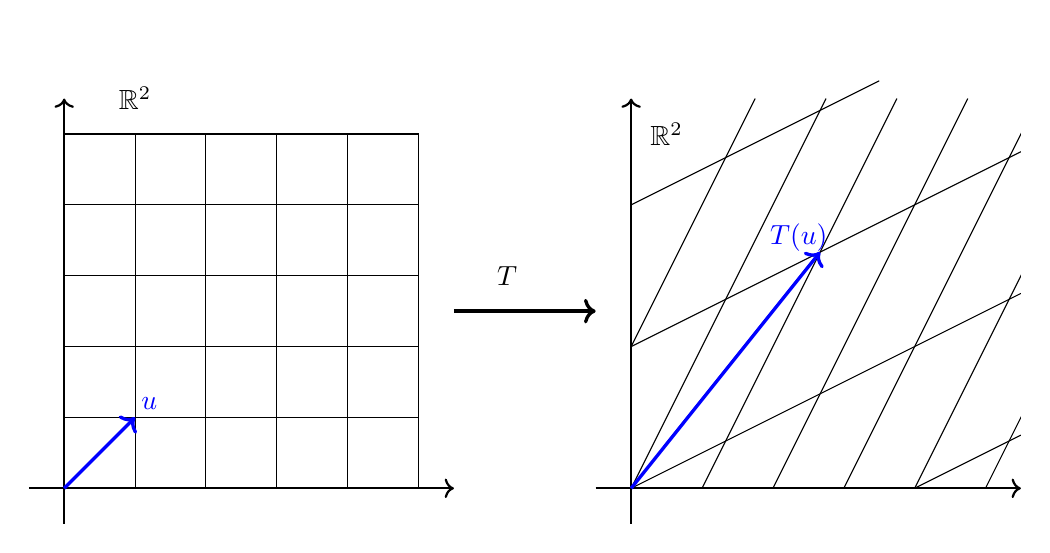
\begin{tikzpicture}[scale=0.9]
      % Left grid (domain)
      \begin{scope}[shift={(-5,0)}]
        % Draw grid
        \draw[step=1cm, black] (0,0) grid (5,5);
        
        % Draw axes
        \draw[thick, ->] (-0.5,0) -- (5.5,0);
        \draw[thick, ->] (0,-0.5) -- (0,5.5);
        
        % Label the space
        \node at (1,5.5) {$\mathbb{R}^2$};
        \draw[->, very thick, blue] (0, 0) -- (1, 1);
        \node[blue] at (1.2,1.2) {$u$};
      \end{scope}
      
      % Transformation arrow
      \draw[->, very thick] (0.5,2.5) -- (2.5,2.5);
      \node at (1.25,3) {$T$};

      
      % Right grid (codomain)
      \begin{scope}[shift={(3,0)}]
        % Draw only axes
        \draw[thick, ->] (-0.5,0) -- (5.5,0);
        \draw[thick, ->] (0,-0.5) -- (0,5.5);
        
        % Label the space
        \node at (0.5,5) {$\mathbb{R}^2$};
        
        % Clip all drawing to stay within visible area
        \begin{scope}
          \clip (-0.5,-0.5) rectangle (5.5,6.5);
          
          % Existing lines with slope 1/2
          \draw[] (4,0) -- (5.5,0.75);
          \draw[] (0,0) -- (5.5,2.75);
          \draw[] (0,2) -- (5.5,4.75);
          \draw[] (0,4) -- (3.5,5.75);
          
          % New lines with slope 2
          \draw[] (5,0) -- (7.75,5.5);
          \draw[] (4,0) -- (6.75,5.5);
          \draw[] (3,0) -- (5.75,5.5);
          \draw[] (2,0) -- (4.75,5.5);
          \draw[] (1,0) -- (3.75,5.5); 
          \draw[] (0,0) -- (2.75,5.5); 
          \draw[] (0,2) -- (1.75,5.5); 
        \end{scope}
        \node[blue] at (2.366,3.533) {$T(u)$};
        \draw[->, very thick, blue] (0, 0) -- (2.666, 3.333);
      \end{scope}
    \end{tikzpicture}
    \caption{We can visualize all linear transformations as "transforming" the axes as shown below. }
    \label{fig:linear_map}
  \end{figure}

  \begin{definition}[Image]
    The \textbf{image}, or \textbf{range} of $T: U \longrightarrow V$ is the image of $U$ under $T$, denoted Im$T$. 
    \begin{equation}
      \im{T} \equiv \{ T(u) \; | \; u \in U\} \subset V
    \end{equation}
    The \textbf{kernel or nullspace} of $T$ is the subset of $U$ that is mapped onto $0$, denoted ker$T$. 
    \begin{equation}
      \text{ker}\,T \equiv \{ u \in U \; | \; T(u) = 0\}
    \end{equation}
  \end{definition}

  \begin{example}
    Let $U_1$ be a subspace of $U$ and given the quotient map
    \begin{equation}
      \pi: U \longrightarrow U / U_1
    \end{equation}
    Then, 
    \begin{equation}
      \text{ker}\,\pi = U_1, \; \im{\pi} = U / U_1
    \end{equation}
    Note that a quotient map is always surjective. 
  \end{example}

  \begin{theorem}[Rank Nullity Theorem]
    Let $T: U \longrightarrow V$ be linear. Then, 
    \begin{equation}
      \dim \ker T + \dim \im T = \dim U
    \end{equation}
    This theorem is quite intuitive, if we visualize the map. 

    \begin{figure}[H]
      \centering 
      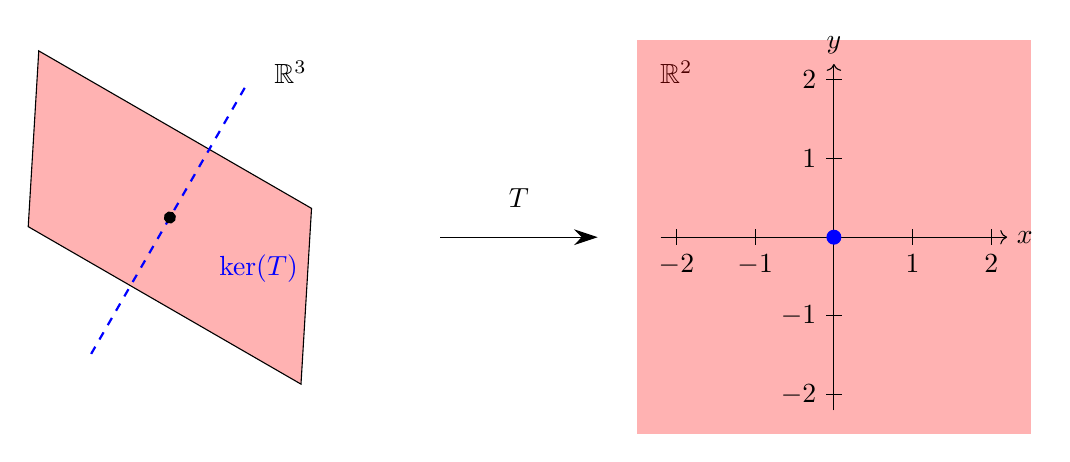
\begin{tikzpicture}
        % Add R³ label for the left side
        \node at (-2.9,2.1) {$\mathbb{R}^3$};
        
        % Add R² label for the right side
        \node at (2,2.1) {$\mathbb{R}^2$};
        
        % Left diagram - Parallelogram with kernel
        \begin{scope}[shift={(-4,0)}]
          % Rotate the entire picture 30 degrees clockwise
          \begin{scope}[rotate=-30]
            % Define coordinates for the parallelogram
            \coordinate (A) at (-2,-1);
            \coordinate (B) at (2,-1);
            \coordinate (C) at (1,1);
            \coordinate (D) at (-3,1);
            
            % Draw the parallelogram with red fill
            \fill[red, opacity=0.3] (A) -- (B) -- (C) -- (D) -- cycle;
            \draw (A) -- (B) -- (C) -- (D) -- cycle;
            
            % Draw the dashed portion where the line intersects the parallelogram in blue
            \draw[dashed, thick, blue] (-0.5,-2) -- (-0.5,2);
            
            % Add a dot at intersection point
            \filldraw (-0.5,0) circle (2pt);
            
            % Label the dashed line in blue
            \node[blue] at (0.8,0) {$\mathrm{ker}(T)$};
          \end{scope}
        \end{scope}
        
        % Arrow connecting the two diagrams
        \draw[-{Stealth[length=3mm,width=2mm]}] (-1,0) -- (1,0);
        \node at (0,0.5) {$T$};
        
        % Right diagram - Real plane
        \begin{scope}[shift={(4,0)}]
          % Fill the background with red
          \fill[red, opacity=0.3] (-2.5,-2.5) rectangle (2.5,2.5);
          
          % Draw the x and y axes
          \draw[->] (-2.2,0) -- (2.2,0) node[right] {$x$};
          \draw[->] (0,-2.2) -- (0,2.2) node[above] {$y$};
          
          % Add tick marks
          \foreach \x in {-2,-1,1,2}
            \draw (\x,0.1) -- (\x,-0.1) node[below] {$\x$};
          \foreach \y in {-2,-1,1,2}
            \draw (0.1,\y) -- (-0.1,\y) node[left] {$\y$};
          
          % Mark the origin with a blue point
          \filldraw[blue] (0,0) circle (2.5pt);
        \end{scope}
      \end{tikzpicture}
      \caption{We just have to realize that given a linear transformation mapping from a $n$-dimensional $V$ to a $m$-dimensional $U$, every vector in $V$ will either get mapped to $0 \in U$ or will get mapped to a nonzero vector in $U$. In this case, the kernel will get mapped to $0$ and everything else is (not always, but in this case) $\mathbb{R}^2$. } 
      \label{fig:rank_nullity}
    \end{figure}
  \end{theorem}

  \begin{proposition}
    Hom$(U, V)$ is the vector space of linear mappings, with addition and scalar multiplication defined
    \begin{align*}
      & (S + T) (x) \equiv S(x) + T(x) \\
      & (c T) (x) \equiv c T(x)
    \end{align*}
  \end{proposition}

  \begin{definition}[Composition]
    The \textbf{composition} of linear functions, denoted with $\circ$, is defined
    \begin{equation}
      (S \circ T) (x) \equiv S\big( T(x)\big)
    \end{equation}
    Given $T \in $ Hom$(U, V)$ and $S \in $ Hom$(V, W)$, then $S \circ T \in $ Hom$(U, W)$. For simplicity, we also denote the composition as 
    \begin{equation}
      S \circ T \equiv S T
    \end{equation}
  \end{definition}

  \begin{proposition}[Composition is Distributive]
    Composition is (right and left) distributive with respect to the addition of linear maps. That is, 
    \begin{align*}
      & (R + S) \circ T = R \circ T + S \circ T \\
      & T \circ (R + S) = T \circ R + T \circ S 
    \end{align*}
  \end{proposition}

  \begin{definition}[Algebra]
    An \textbf{algebra} $A$ is a vector space with the additional operation of vector multiplication. That is, $A$ is closed under 
    \begin{equation}
      \circ: A \times A \longrightarrow A
    \end{equation}
    An algebra is \textbf{associative} if multiplication is associative. That is, given $R, S, T \in A$
    \begin{equation}
      R \circ (S \circ T) = (R \circ S) \circ T
    \end{equation}
    Note that multiplication is not necessarily commutative. 
  \end{definition}

  \begin{proposition}
    End$(V)$ is an associative, noncommutative algebra. 
  \end{proposition}

  \begin{example}
    A rotation around any axis or a flip across any hyperplane is an element of End$(\mathbb{R}^n)$. 
  \end{example}

  \begin{definition}[Projection]
    A \textbf{projection mapping} is a linear mapping $P$ where 
    \begin{equation}
      P = P^2
    \end{equation}
  \end{definition}

  \begin{example}
    Let $P$ be an orthogonal projection mapping onto a subspace $Y$ of $X$. $\im P = Y$, and $\ker P = Y^\perp$ or the span of vectors in $X$ that are "orthogonal" to $Y$. Note that we haven't actually endowed a structure onto $X$ to even define orthogonality yet, so this definition is purely visual and not mathematically rigorous. 
  \end{example}

  \begin{example}
    Reflections, projections, shears, and rotations are all linear maps. Differentiation and integration are also examples of linear mappings. 
  \end{example}

  Linear maps over vector spaces over different fields are generally not well defined since the definition of homomorphisms do not cover the fields in which vector spaces are associated with. 

  \begin{theorem}
    Given $A: V \longrightarrow U$ a linear mapping between vector spaces and $b \in U$, all solutions to the equation $Ax = b$ is in $a + \ker A$, that is, of the form 
    \begin{equation}
      x = a + y, \; y \in \ker A
    \end{equation}
    where $x = a$ is one solution. 
  \end{theorem}

  \begin{corollary}
    A linear map $A$ is injective if and only if $\ker A = 0$.
  \end{corollary}

  \begin{definition}[Rank]
    The \textbf{rank} of a linear map $A$ is the dimension of its image. 
  \end{definition}

\subsection{Factorization of Linear Maps}

  \begin{definition}[Restriction]
    Let $\varphi: U \longrightarrow V$ be a linear mapping and let $U_1 \subset U, V_1 \subset V$ be subspaces. Such that 
    \begin{equation}
      \varphi u \in V \text{ for all } u \in U
    \end{equation}
    Then, the linear mapping 
    \begin{equation}
      \varphi_1: U_1 \longrightarrow V_1, \; \varphi_1 u = \varphi_u, u \in U_1
    \end{equation}
    is called the \textbf{restriction} of $\varphi$ to $U_1, V_1$. It suffices the identity
    \begin{equation}
      \varphi \circ i_U = i_V \circ \varphi_1
    \end{equation}
    where $i_U: U_1 \longrightarrow U, i_V: V_1 \longrightarrow V$ are canonical injections. Equivalently, we say that the diagram below is \textbf{commutative}. 
    \[
      \begin{tikzcd}
        U \arrow{r}{\varphi} & V \\
        U_1 \arrow{u}{i_U} \arrow{r}{\varphi_1} & V_1 \arrow{u}{i_V}
      \end{tikzcd}
    \]
    We can also define 
    \begin{equation}
      \varphi_1 \equiv i_v^{-1} \varphi i_U
    \end{equation}
  \end{definition}

  The construction of the restriction is an enormously helpful tool for many proofs and very useful for factoring linear mappings. 

  \begin{definition}[Induced Mapping of Quotients]
    Given $\varphi: U \longrightarrow V$ with quotient maps 
    \begin{equation}
      \pi_U: U \longrightarrow U / U_1, \; \pi_V: V \longrightarrow V / V_1
    \end{equation}
    the \textbf{induced mapping of the quotient spaces} is the unique mapping $\bar{\varphi}: U/U_1 \longrightarrow V / V_1$ such that 
    \begin{equation}
      \bar{\varphi} \circ \pi_U = \pi_V \circ \varphi
    \end{equation}
    or equivalently, the following diagram commutes. 
    \[\begin{tikzcd}
        U \arrow{r}{\varphi} \arrow{d}{\pi_U} & V \arrow{d}{\pi_V}\\
        U / U_1 \arrow{r}{\bar{\varphi}} & F / F_1
    \end{tikzcd}\]
  \end{definition} 

  \begin{theorem}
    Every linear mapping can be written as the composition of a surjective mapping followed by an injective mapping. That is, every $A$ can be factored into 
    \begin{equation}
      A = A_{inj} \circ A_{surj}
    \end{equation}
  \end{theorem}
  \begin{proof}
    We can induce a quotient mapping to construct a factoring of a linear mapping. We can define the unique mapping 
    \begin{equation}
      \bar{\varphi}: U / \ker{U} \longrightarrow F
    \end{equation}
    such that, $\varphi = \bar{\varphi} \circ \pi_U$, or that 
    \[\begin{tikzcd}
       U \arrow{r}{\varphi} \arrow{d}{\pi_U} & V \\
       U / \ker{\varphi} \arrow{ru}{\bar{\varphi}}
    \end{tikzcd} \]
    commutes. Clearly, $\bar{\varphi}$ is injective since if it were not, $\bar{\varphi} \pi_U x = 0 \implies \varphi x = 0 \implies x \in \ker{\varphi} \implies \pi_U x = 0$. This also means that the restriction of $\bar{\varphi}$ to $U / \ker{\varphi}$
    \begin{equation}
      \bar{\bar{\varphi}}: U / \ker{\varphi} \longrightarrow \im{\varphi}
    \end{equation}
    is a linear isomorphism. Thus, for any $\varphi$, it can be written as $\bar{\varphi} \circ \pi_U$, with $\bar{\varphi}$ injective and $\pi_U$ surjective. 
  \end{proof}

  \begin{proposition}
    Given $E_1, E_2$ subspaces of $E$. Then, 
    \begin{equation}
      \frac{E_1}{E_1 \cap E_2} \simeq \frac{E_1 + E_2}{E_2}
    \end{equation}
    In fact, they are naturally isomorphic. 
  \end{proposition}
  \begin{proof}
    $E_1 + E_2$ can be decomposed to $E_1^\prime \oplus (E_1 \cap E_2) \oplus E_2^\prime$, where $E_1^\prime$ consists of the subspace of vectors $x$ that can only be expressed as $x = x_1, x_1 \in E_1$ and $E_2^\prime$ are vectors that can only be expressed as $x = x_2, x_2 \in E_2$. Define the projection mapping
    \begin{equation}
      \text{proj}: E_1 + E_2 \longrightarrow E_1^\prime
    \end{equation}
    Since $E_1 = E_1^\prime \oplus (E_1 \cap E_2)$, we can define the natural isomorphism 
    \begin{equation}
      \kappa: E_1^\prime \longrightarrow \frac{E_1}{E_1 \cap E_2}, \; \kappa{x} = \{x\}
    \end{equation}
    We now define the mapping $\varphi: E_1^\prime \longrightarrow (E_1 + E_2) / E_2$ such that
    \begin{equation}
      \pi = \varphi \text{proj}
    \end{equation}
    given by the diagram 
    \[\begin{tikzcd} 
        E_1 + E_2 \arrow{d}{proj} \arrow{r}{\pi} & \frac{E_1 + E_2}{E_2} \\
        E_1^\prime \arrow{ru}{\varphi} \arrow{r}{\kappa} & \frac{E_1}{E_1 \cap E_2}
    \end{tikzcd}\]
    Such a $\varphi$ exists because proj is surjective and can thus be inverted. We now claim that $\varphi$ is an isomorphism. $\ker{\text{proj}} = \ker{\pi} = E_2 \implies \kappa$ is injective. Given $x = x_1 + y + x_2 \in E_1 + E_2$ such that $x_1 \in E_1^\prime, y \in E_1 \cap E_2, x_2 \in E_2^\prime$, 
    \begin{equation}
      \pi(x) = \pi(x_1 + y + x_2) = \pi(x_1) = \varphi \text{proj} (x_1) = \varphi (x_1)
    \end{equation}
    meaning that for every vector $v \in (E_1 + E_2) / E_2$, it can be expressed as $v = \pi (x) = \varphi (x_1)$, meaning that there exists a $x_1 \in E_1^\prime$ mapping to $v$ under $\varphi \iff \varphi$ is surjective. So, $\varphi$ is an isomorphism $\implies \varphi \kappa^{-1}$ is an isomorphism.  
  \end{proof}

  \begin{corollary}
    In the special case when $E_1 \oplus E_2 = E$, then the proposition states that 
    \begin{equation}
      E_1 \simeq \frac{E}{E_2}
    \end{equation}
  \end{corollary}

  Let $f_1, f_2, ..., f_n$ be any $n$ linear functionals of $U$. Define the subspace $F \subset E$ as 
  \begin{equation}
    F \equiv \bigcap_{i=1}^n \ker{f_i}
  \end{equation}
  and define linear map 
  \begin{equation}
    \phi: U \longrightarrow \mathbb{F}^n, \;\phi(x) \equiv (f_1(x), f_2(x), ..., f_n(x))
  \end{equation}
  $\implies \ker{\phi} = F$. So, $\phi: U \longrightarrow \mathbb{F}^n$ defines the isomorphism 
  \begin{equation}
    \bar{\phi}: U / F \longrightarrow \im{\phi}
  \end{equation}

  \begin{proposition}
    Given linear mappings $\phi: E \longrightarrow F$, $\psi: E \longrightarrow G$ such that
    \begin{equation}
      \ker{\phi} \subseteq \ker{\psi}
    \end{equation}
    Then there exists a map $\kappa$ such that 
    \begin{equation}
      \psi = \kappa \phi
    \end{equation}
    or equivalently, such that the diagram below commutes. 
    \[\begin{tikzcd} 
        E \arrow{r}{\phi} \arrow{d}{\psi} & F \arrow{dl}{\kappa} \\
        G 
    \end{tikzcd}\]
  \end{proposition}

  Now, we introduce the concept of exact sequences which is useful in the factoring of linear maps. Note that exact sequences are used in group theory to factor transformation groups. 

  \begin{definition}
    A sequence of linear mappings 
    \begin{equation}
      F \xrightarrow{\varphi} E \xrightarrow{\psi} G
    \end{equation}
    is \textbf{exact at E} if
    \begin{equation}
      \im{\varphi} = \ker{\psi}
    \end{equation}
  \end{definition}

  Notice that if we have an exact sequence 
  \begin{equation}
    0 \xrightarrow{\varphi} E \xrightarrow{\psi} G
  \end{equation}
  then, $0 = \im{\varphi} = \ker{\psi} \implies \psi$ is injective. If we have exact sequence 
  \begin{equation}
    F \xrightarrow{\varphi} E \xrightarrow{\psi} 0
  \end{equation}
  then, $\im{\varphi} = \ker{\psi} = E \implies \varphi$ is surjective. 

  \begin{definition}
    A \textbf{short exact sequence} is a sequence of the form
    \begin{equation}
      0 \xrightarrow{} F \xrightarrow{\varphi} E \xrightarrow{\psi} G \xrightarrow{} 0
    \end{equation}
    such that it is exact at $F, E$, and $G$. It is clear that the first and last maps are the zero maps. With this definition, we can easily prove that
    \begin{enumerate}
      \item $\varphi$ is injective
      \item $\psi$ is surjective
      \item $E / \im{F} \simeq G$
    \end{enumerate}
  \end{definition}

  \begin{example}
    The sequence 
    \begin{equation}
      0 \xrightarrow{} E_1 \xrightarrow{i} E \xrightarrow{\pi} E / E_1 \xrightarrow{} 0
    \end{equation}
    is exact, where $i$ denotes the canonical injection and $\pi$ the canonical projection. This example is the only example of an exact sequence between vector spaces up to isomorphism. 
  \end{example}

  \begin{definition}
    A commutative diagram of the form
    \[\begin{tikzcd}
        0 \arrow{r} & F_1 \arrow{d}{\alpha} \arrow{r}{\varphi_1} & E_1 \arrow{d}{\beta} \arrow{r}{\psi_1} & G_1 \arrow{d}{\gamma} \arrow{r} & 0 \\
        0 \arrow{r} & F_2 \arrow{r}{\varphi_2} & E_2 \arrow{r}{\psi_2} & G_2 \arrow{r} & 0 
    \end{tikzcd}\]
    where both horizontal sequences are short exact sequences and $\alpha, \beta, \gamma$ are homomorphisms between linear spaces is a \textbf{homomorphism of exact sequences}. If $\alpha, \beta, \gamma$ are linear isomorphisms, then this is an \textbf{isomorphism of exact sequences}. 
  \end{definition}

  \begin{proposition}
    A short exact sequence of vector spaces
    \begin{equation}
      0 \xrightarrow{} F \xrightarrow{\varphi} E \xrightarrow{\psi} G \xrightarrow{} 0
    \end{equation}
    is split if it essentially presents $E$ as the direct sum of groups $F$ and $G$. That is, there exists an isomorphism of exact sequences.
    \[\begin{tikzcd}
        0 \arrow{r} & F \arrow{d}{\alpha} \arrow{r}{\varphi_1} & E \arrow{d}{\beta} \arrow{r}{\psi_1} & G \arrow{d}{\gamma} \arrow{r} & 0 \\
        0 \arrow{r} & F \arrow{r}{\varphi_2} & F \oplus G \arrow{r}{\psi_2} & G \arrow{r} & 0 
    \end{tikzcd}\]
    or equivalently, there exists an isomorphism between $E$ and $F \oplus G$. 
  \end{proposition}

  \begin{definition}
    Given a short exact sequence
    \begin{equation}
      0 \xrightarrow{} F \xrightarrow{\varphi} E \xrightarrow{\psi} G \xrightarrow{} 0
    \end{equation}
    if there exists a map $\kappa: G \longrightarrow E$, such that $ \psi \circ \kappa = I$, then the sequence is said to be a \textbf{split short exact sequence}, written
    \begin{equation}
      0 \xrightarrow{} F \xrightarrow{\varphi} E \xleftrightarrow{\psi, \kappa} G \xrightarrow{} 0
    \end{equation}
  \end{definition}

  \begin{proposition}
    Every short exact sequence can be split. 
  \end{proposition}
  \begin{proof}
    It will be proved later that $\psi$ is surjective $\implies$ $\psi$ is left invertible. 
  \end{proof}

  \begin{definition}[Stable Subspaces]
    Given $\varphi: E \longrightarrow E$, a subspace $E_1 \subset E$ is called \textbf{stable} 
    \begin{equation}
      x \in E_1 \implies \varphi x \in E_1
    \end{equation}
    That is, the restriction of $\varphi$ to $E_1$, denoted
    \begin{equation}
      \varphi: E_1 \longrightarrow E_1
    \end{equation}
    is well-defined. Clearly, $\im{\varphi}$ and $\ker{\varphi}$ is stable, and the induced map 
    \begin{equation}
      \bar{\varphi}: E / E_1 \longrightarrow E / E_1
    \end{equation}
    is a linear endomorphism of $E / E_1$. 
  \end{definition}

  We end this subsection by defining the induced linear map from the direct sum of spaces. 

  \begin{definition}
    Given linear maps $A_i \in$ End$(V_i)$ for $i = 1, 2, ..., n$, the induced linear map
    \begin{equation}
      \bigoplus_{i =1}^n A_i: \bigoplus_{i=1}^n V_i \longrightarrow \bigoplus_{i=1}^n V_i
    \end{equation}
    is defined
    \begin{equation}
      (\bigoplus_{i=1}^n A_i)(\bigoplus_{i=1}^n x_i) \equiv \bigoplus_{i=1}^n A_i x_i
    \end{equation}
  \end{definition}

\subsection{Invertibility and Transpose}

  We now introduce the concepts of left and right invertibility of linear mappings. 

  \begin{theorem}[Left/Right-Invertibility]
    A linear mapping $T: U \longrightarrow V$, with $\dim{U} = n, \dim{V} = m$, is \textbf{left-invertible}. That is, there exists linear $S$ such that 
    \begin{equation}
      S T = I
    \end{equation}
    if and only if $T$ is injective $\iff$ rank$(T) = n$. Linear $T$ is \textbf{right-invertible}, that is, there exists linear $S$ such that 
    \begin{equation}
      T S = I
    \end{equation}
    if and only if $T$ is surjective $\iff$ rank$(T) = m$. 
  \end{theorem}
  \begin{proof}
    We will only prove the case for left-invertibility. Right invertibility follows analogously. 
    \begin{enumerate}
      \item $(\leftarrow)$ $T$ is injective $\implies$ rank$(T) = \dim{U} = \dim{\im{T}}$. Let $(\im{T})^\prime$ exist such that 
      \begin{equation}
        \im{T} \oplus (\im{T})^\prime = V
      \end{equation}
      We define the isomorphism 
      \begin{equation}
        \Tilde{T}: V \longrightarrow \im{T}
      \end{equation}
      and then define $S$. Given that $v = w + w^\prime \in V$, with $w \in \im{T}, w^\prime \in (\im{T})^\prime$, 
      \begin{equation}
        S : V \longrightarrow U, \; S(v) \equiv \Tilde{T}^{-1} (v)
      \end{equation}
      $\implies S T (u) = \Tilde{T}^{-1} T (u) = u \iff S T = I$. 

      \item $(\rightarrow)$ We prove the contrapositive. $T$ is not injective $\implies \dim{\ker{T}} > 0 \implies $ there exists 2 linearly independent vectors $x, y \in U$ such that
      \begin{equation}
        T x = T y
      \end{equation}
      Assume that a left inverse $S$ exists. Then 
      \begin{equation}
        x = S T x = S T y = y \implies x = y
      \end{equation}
      leading to a contradiction $\implies$ the left-inverse does not exist. 
    \end{enumerate}
  \end{proof}

  \begin{definition}[Inverse]
    The inverse of a linear map $A$, denoted $A^{-1}$ is a unique linear map satisfying 
    \begin{equation}
      A A^{-1} = A^{-1} A = I
    \end{equation}
    where $I$ is the identity map. 
  \end{definition}

  \begin{corollary}
    A linear map is invertible if and only if it is an isomorphism. 
  \end{corollary}

  We finally end this section by defining the transpose of a linear mapping. 

  \begin{definition}[Transpose]
    Given a linear mapping $A: U \longrightarrow V$, let there exist a certain $\varphi \in V^*$. Then, there exists a corresponding $l \in U^*$ such that 
    \begin{equation}
      l \equiv \varphi A
    \end{equation}
    This mapping $A^T: V^* \longrightarrow U^*$ that assigns every $\varphi$ to a corresponding $l$ is called the \textbf{transpose} of $A$. Note that the transpose is canonically formed when defining any linear map. We do not need any additional structure on $U$ or $V$ to define $A^T$.
    \[
      \begin{tikzcd}
        U \arrow{r}{A} \arrow[swap]{dr}{l = \varphi A} & V \arrow{d}{\varphi} \\
        & \mathbb{F}
      \end{tikzcd}
    \]
  \end{definition}

  It is worth mentioning that $A^T$ maps every element in the annihilator $V^0$ to an element in $U^0$, but not necessarily the other way around. 

  \begin{theorem}
    \begin{equation}
      (\im A)^0 = \ker A^T \text{ or equivalently, } \im A = (\ker A^T)^0
    \end{equation}
  \end{theorem}


\section{Metrics, Norms, and Inner Products} 

  Given a vector space $V$, we can induce different structures on it to allow us to conduct different measurements on it. For example, the endowment of the basis structure on $V$ allows us to represent vector as an $n$-tuple of scalars. Some structures may induce other structures, such as the inner product inducing a norm or a metric inducing a norm. We will begin by defining these structures. It must be further noted that in order to induce such structures on $V$, its base field $\mathbb{F}$ must be ordered. We will treat $\mathbb{F} = \mathbb{C}$ for the following definitions. 

  \begin{definition}[Metric]
    A \textbf{metric} on a vector space $V$ over field $\mathbb{C}$ is a mapping
    \begin{equation}
      d: V \times V \longrightarrow \mathbb{R}
    \end{equation}
    satisfying three properties 
    \begin{enumerate}
      \item $d(x, y) = d(y, x)$
      \item $d(x, y) \geq 0$, with $d(x,y) = 0 \iff x=y$
      \item $d(x, y) + d(y,z) \geq d(x,z)$
    \end{enumerate}
    A metric allows us to define some notion of distance in $V$. A vector space $V$ with a metric is called a \textbf{metric space}, denoted $(V, d)$. 
  \end{definition}

  \begin{definition}[Norm]
    A \textbf{norm} on a vector space $V$ over field $\mathbb{C}$ is a mapping 
    \begin{equation}
      \rho: V \longrightarrow \mathbb{R}
    \end{equation}
    satisfying three properties 
    \begin{enumerate}
      \item $\rho (x) \geq 0$, with $\rho(x) = 0 \iff x = 0$
      \item For $a \in \mathbb{C}$, $\rho (a x) = |a| \rho(x)$ 
      \item $\rho(x + y) \leq \rho(x) + \rho(y)$ 
    \end{enumerate}
    A norm allows us to define some notion of a magnitude or length on each vector in $V$. A vector space $V$ with a norm is called a \textbf{normed space}, denoted $(V, \rho)$. 
  \end{definition}

  \begin{example}[Absolute Value]
    The absolute value function $|\cdot|: \mathbb{C} \longrightarrow \mathbb{R}_+$ is an example of a norm on the 1 dimensional space $\mathbb{C}$. 
  \end{example}

  \begin{example}[Euclidean Norm, $L_2$-Norm]
    The Euclidean norm of a vector $x \equiv (x_1, x_2, ..., x_n)^T \in \mathbb{R}^n$ is defined
    \begin{equation}
      ||x||_2 \equiv \bigg( \sum_{i=1}^n x_i^2 \bigg)^{\frac{1}{2}}
    \end{equation}
    This is the most commonly used norm in $\mathbb{R}^n$. 
  \end{example}

  \begin{example}[Taxicab Norm, Manhattan Norm]
    The Taxicab norm of $x \equiv (x_1, x_2, ..., x_n)^T \in \mathbb{R}^n$ is defined
    \begin{equation}
      ||x||_1 \equiv \sum_{i=1}^n |x_i|
    \end{equation}
  \end{example}

  \begin{example}[Infinity Norm, $L_\infty$-Norm]
    The Infinity norm of vector $x \equiv (x_1, x_2, ..., x_n)^T \in \mathbb{R}^n$ is defined
    \begin{equation}
      ||x||_\infty \equiv \max{\{|x_1|, |x_2|, ..., |x_n|\}}
    \end{equation}
  \end{example}

  \begin{example}[p-norm, $L_p$-Norm]
    Let $p\geq 1$ be a real number. The p-norm of a vector 
    \begin{equation}
      x \equiv (x_1, x_2, ..., x_n)^T \in \mathbb{R}^n
    \end{equation}
    is defined
    \begin{equation}
      ||x||_p \equiv \bigg( \sum_{i=1}^n x_i^p \bigg)^{\frac{1}{p}}
    \end{equation}
    For $0<p<1$, this function could be of some use, but it is not considered a norm since it violates the triangle inequality. When $p = 1$ and $p =2$, the norm is the Taxicab norm and Euclidean norm, respectively, and 
    \begin{equation}
      \lim_{p \rightarrow \infty} ||\cdot||_p = ||\cdot||_\infty
    \end{equation}
  \end{example}

  \begin{definition}[Seminorm]
    A \textbf{seminorm}, or a pseudo-norm, has the same properties except that $\rho(x) = 0$ does not necessarily imply that $x = 0$. That is, nonzero vectors can have norms of $0$. 
  \end{definition}

  \begin{theorem}[Norm Induces Metric]
    Every norm induces a metric in the following way
    \begin{equation}
      d(x, y) \equiv \rho(x-y)
    \end{equation}
    However, a metric does not necessarily induce a norm because the definition
    \begin{equation}
      \rho(x) \equiv d(x, 0)
    \end{equation}
    is not guaranteed to have all properties of the norm. 
  \end{theorem}

  \begin{definition}[Inner Product]
    An \textbf{inner product} on a vector space $V$ over field $\mathbb{C}$ is a mapping 
    \begin{equation}
      (\cdot, \cdot): V \times V \longrightarrow \mathbb{R}
    \end{equation}
    satisfying three properties 
    \begin{enumerate}
      \item First Argument Linearity: $(\lambda x + \mu y, z) = \lambda (x, z) + \mu (y, z)$
      \item Conjugate symmetry: $(x, y) = \bar{(y, x)}$
      \item $(x, y) \geq 0$, with $(x, y) = 0 \iff x = y$
    \end{enumerate}
    An inner product allows us to define some notion of an angle between two vectors in $V$. A vector space $V$ with an inner product is called an \textbf{inner product space}. Note that when the field is $\mathbb{C}$, the inner product is \textbf{sesqui-linear}, that is, linear with respect to the first argument and \textbf{skew linear} with respect to the second. When $\mathbb{R}$, it is bilinear. 
  \end{definition}

  The inner product of a vector space $V$ over $\mathbb{R}$ is an element of $V^* \otimes V^*$. This concept of the metric tensor occurs when studying Riemannian manifolds in general relativity. 

  \begin{definition}[Inner Product Induces Norm]
    An inner product induces a norm in the following way
    \begin{equation}
      ||x|| \equiv \sqrt{(x,x)} 
    \end{equation}
  \end{definition}

  \begin{theorem}[Schwarz Inequality]
    For all $x, y \in V$, 
    \begin{equation}
      |(x, y)| \leq ||x|| ||y||
    \end{equation}
  \end{theorem}

  \begin{example}[Dot Product]
    Given vectors $x, y \in \mathbb{R}^n$, 
    \begin{equation}
      x \cdot y \equiv  \begin{pmatrix}
      x_1\\x_2\\\vdots\\x_n
      \end{pmatrix} \cdot \begin{pmatrix}
      y_1\\y_2\\\vdots\\y_n
      \end{pmatrix} \equiv \sum_{i=1}^n x_i y_i
    \end{equation}
  \end{example}

  \begin{example}[Integral Product]
    Let $C^0[a, b]$ be the space of all continuous real-valued functions defined over the interval $[a,b] \subset \mathbb{R}$. Given $f, g \in C^0[a,b]$, 
    \begin{equation}
      (f, g) \equiv \int_a^b f(x)g(x) d x
    \end{equation}
    is an inner product on $C^0[a, b]$. 
  \end{example}

  \begin{theorem}[Pythagorean Theorem]
    \begin{equation}
      ||x||^2 + ||y||^2 = ||x+y||^2
    \end{equation}
  \end{theorem}

  \begin{theorem}
    \begin{equation}
      ||x|| = \max_{||y||=1} (x, y)
    \end{equation}
  \end{theorem}

  \begin{definition}[Orthogonal Vectors]
    Two vectors $x, y$ of an inner product space are said to be \textbf{orthogonal} if 
    \begin{equation}
      (x, y) = 0
    \end{equation}
  \end{definition}

  Note that the definition of orthogonality is dependent on the definition of the inner product. If the inner product is defined differently, then orthogonality will be defined differently. In the case when the inner product is defined to be the dot product, orthogonality is defined to be the "normal" perpendicularity between vectors. We can further define subspaces to be orthogonal. 

  \begin{definition}[Orthogonal Subspaces]
    Two subspaces $Y, Z$ of inner product space $Z$ are said to be orthogonal to each other if 
    \begin{equation}
      (y, z) = 0 \text{   for every } y \in Y, z \in Z
    \end{equation}
  \end{definition}

  \begin{definition}[Orthogonal Complement]
    Given a subspace $Y$ of inner product space $X$, the \textbf{orthogonal complement} of $Y$, denoted $Y^\perp$, is defined
    \begin{equation}
      \{ x \in X \; | \; (x, y) = 0 \;\;\; \forall y \in Y\}
    \end{equation}
    which is the set of all vectors in $X$ orthogonal to every vector in $Y$. Clearly, $Y \oplus Y^\perp = X$. 
  \end{definition}

  The concept of orthogonality also allows us to define orthogonal projections onto a vector or subspace. 

  \begin{definition}[Orthogonal Projectjion]
    Let $x \in X$ and let $Y$ be a subspace of $X$. Then $x$ can be decomposed into the form $x = y + z, \; y \in Y, z \in Y^\perp$. The \textbf{orthogonal projection} of $x$ onto $Y$ is then defined as 
    \begin{equation}
      \text{proj}_Y (x) = y
    \end{equation}
    Orthogonal projections are linear transformations. 
  \end{definition}

  \begin{theorem}
    Given that $x \in \mathbb{R}^n$ is projected onto a 1-dimensional subspace $Y$. The orthogonal projection of $x$ onto $Y$ can be computed with the formula 
    \begin{equation}
      \text{proj}_Y (x) = \frac{x \cdot y}{||y||^2} y
    \end{equation}
    where $y$ is an arbitrary vector in $Y$ and $\cdot$ is the dot product in $\mathbb{R}^n$. Furthermore, for a $k$-dimensional subspace $Y$, we can calculate the projection by first adding up the projections of $x$ onto a set of basis vectors of $Y$ and then adding them up. That is, given basis $r_1, r_2, ..., r_k$ of $Y$,
    \begin{equation}
        \text{proj}_Y (x) = \sum_{i=1}^k \text{proj}_{r_i} (x) = \sum_{i=1}^k \frac{x \cdot r_i}{||r_i||^2} r_i 
    \end{equation}
  \end{theorem}

  \begin{theorem}[Orthonormal Basis in Hilbert Space]
    Every inner product space has a basis consisting of vectors that are pairwise orthogonal, called an \textbf{orthogonal basis}. Furthermore, each vector in the orthogonal basis can be scaled to have magnitude 1, forming an \textbf{orthonormal basis}.  
  \end{theorem}

  \begin{proof}
    The algorithm used to construct an orthonormal basis is called \textbf{Grahm-Schmidt}. We start off with any basis, not necessarily orthonormal, of $X$, denoted $\{x_1, x_2, ..., x_n\}$. We first assign 
    \begin{equation}
      x_1 = l_1
    \end{equation}
    Then we take $x_2$ and find the orthogonal component (with respect to $l_1$) with the equation
    \begin{equation}
      l_2 = x_2 - \text{proj}_{l_1} (x_2)
    \end{equation}
    This creates an orthogonal basis for span$\{x_1, x_2\}$. Then we take $x_3$ and find the orthogonal component (with respect to span$\{l_1, l_2\}$. 
    \begin{equation}
      l_3 = x_3 - \text{proj}_{l_1} (x_3) - \text{proj}_{l_2} (x_3)
    \end{equation}
    This creates an orthogonal basis for span$\{x_1, x_2, x_3\}$. We repeat this process until we complete the basis of $X$, using the general equation
    \begin{equation}
      l_k = x_k - \sum_{i=1}^{k-1} \text{proj}_{l_k} (x_k) = x_k - \sum_{i=1}^{k-1} \frac{x_k \cdot l_k}{||l_k||^2} l_k, \; k = 1, 2, ..., n
    \end{equation}
    Finally, we take these orthogonal vectors and normalize them to magnitude 1. Note that this algorithm does not produce a unique orthonormal basis. Rather, it is highly un-unique. 
  \end{proof}

  Given that we have an orthonormal basis $\{r_i\}_{i=1}^k$ of subspace $Y$ in $\mathbb{R}^n$, we can more simply define 
  \begin{equation}
    \text{proj}_Y (x) = \sum_{i=1}^k (x \cdot r_i) r_i
  \end{equation}

  \begin{theorem}
    The inner product endowed on $V$ induces a natural isomorphism between $V$ and $V^\ast$. 
  \end{theorem}
  \begin{proof}
    We fix $y \in V$ and simply define the isomorphism to be. 
    \begin{equation}
      l(y) \equiv (x, y)
    \end{equation}
    which defines a bijection between $x \in V$ and $l \in V^*$. 
  \end{proof}

  Note that given vector spaces $U, V$, the set of all linear mappings $A: U \longrightarrow V$ also forms a vector space. More specifically, it is a rank (1,1) tensor product space. This means that we can define similar Euclidean structures on them. The norm of a matrix is worth mentioning. Note that the structures and concepts of metrics, norms, inner products, distances, magnitudes, orthogonality, and basis are not intrinsic properties of the vector space. So, we will not assume the existence of these structures unless otherwise stated or explicitly implied. 


\section{Matrices}

\subsection{Representations of Linear Maps} 

  We now describe the construction of the matrix realization of a linear map from $V \longrightarrow U$. In order to do this, we \textit{must} define a basis for each $V$ and $U$. If $V = U$, then we usually define the same basis for both the domain and codomain. 

  Let the basis for $U$ be $\{ u_1, u_2, ..., u_n\}$ and the basis of $V$ be $\{v_1, v_2, ..., v_m\}$. In fact, the assignment of this specific basis is a linear map in of itself. That is, 
  \begin{align*}
    i: U \longrightarrow \mathbb{F}^n, & i(u_\alpha) = e_\alpha  \\
    j: V \longrightarrow \mathbb{F}^m, & j(v_\beta) = e_\beta 
  \end{align*}
  However, we do not usually include this transformation in the notation. We just denote $i(u)$ as $u$ and $j(v)$ as $v$. Every vector $u \in U$ can then be represented as a linear combination
  \begin{equation}
    u = \sum_{j=1}^n c_j u_j
  \end{equation}
  By linearity of the mapping $A: U \longrightarrow V$, 
  \begin{equation}
    A u = A \bigg( \sum_{j=1}^n c_j u_j \bigg) = \sum_{j=1}^n c_j A u_j 
  \end{equation}
  This means that $A$ can be completely, uniquely determined by defining how it maps the $n$ basis vectors $u_j \in U$, that is, by defining the values 
  \begin{equation}
    A u_1, A u_2, ..., A u_{n-1}, A u_n
  \end{equation}
  Each $A u_j$ will be an element of $V$, which means that $A u_j$ can be decomposed into the linear combination of $v_i$'s. That is, 
  \begin{equation}
    A u_j = \sum_{i=1}^m a_{i j} v_i, \; j = 1, 2, ..., n 
  \end{equation}
  We are done. Given the basis of the domain and codomain, the elements $a_{i j}$ are precisely the entries of the $m \times n$ matrix $(1 \leq i \leq m, 1 \leq j \leq n)$. 
  \begin{equation}
    v = A u \iff 
    \begin{pmatrix}
     b_1 \\ b_2 \\ \vdots \\ b_m
    \end{pmatrix}
    = \begin{pmatrix}
     a_{1 1} & a_{1 2} & \ldots & a_{1 n} \\
     a_{2 1} & a_{2 2} & \ldots & a_{2 n} \\
     \vdots & \vdots & \ddots & \vdots \\
     a_{m 1} & a_{m 2} & \ldots & a_{m n} 
    \end{pmatrix} \begin{pmatrix}
     c_1 \\ c_2 \\ c_3 \\ \vdots \\ c_n
    \end{pmatrix}
  \end{equation}

  It is important to note that the matrix is \textit{not} $A$ in of itself. In the most rigorous sense, the matrix $A$ is really just equal to the composition of mappings $ j^{-1} A i$, but for simplicity it is just written as $A$. It is just one representation of a linear map given the two bases of the domain and codomain. Furthermore, as soon as one writes down a matrix to represent a linear map, they are automatically assuming some choice of basis given by $i$ and $j$. 

  \begin{definition}
    The \textbf{algebra} of $n \times n$ matrices over field $\mathbb{F}$, denoted Mat$(n, \mathbb{F})$, is defined with regular matrix addition and multiplication. 
  \end{definition}

  Furthermore, we can define the mapping between linear operators $T: \mathbb{F}^n \longrightarrow \mathbb{F}^m$ and $m \times n$ matrices (given that there is a basis for both $\mathbb{F}^n, \mathbb{F}^m$. 

  \begin{definition}
    The linear mapping between the algebras 
    \begin{equation}
      \rho: \text{Hom}(\mathbb{F}^n, \mathbb{F}^m) \longrightarrow \text{Mat}(m \times n, \mathbb{F})
    \end{equation}
    is a multiplicative group homomorphism. This mapping that assigns abstract group elements of linear mappings to matrices is called a \textbf{representation}. 
  \end{definition}

  \begin{theorem}
    Mat$(n, \mathbb{F}) \simeq $ End$(\mathbb{F}^n)$ 
  \end{theorem}
  \begin{proof}
    A matrix is completely determined by the basis mapping $i$. By definition, a linear mapping over $\mathbb{F}$ is a basis mapping if and only if it is an element of End$(\mathbb{F}^n)$. 
  \end{proof}

  Note that the composition operation in the algebra of linear operators is realized as the operation of matrix multiplication. These are two distinct operations that are related only through the basis mappings $i$ and $j$. 

  \begin{example}
    Let $\alpha: \mathbb{R}^2 \longrightarrow \mathbb{R}^2$ be the linear transformation of the counterclockwise rotation by $\theta$ and $\beta: \mathbb{R}^2 \longrightarrow \mathbb{R}^2$ be the counterclockwise rotation of $\phi$. Then the matrix representation of $\alpha \circ \beta$ is 
    \begin{align}
        & \begin{pmatrix}
      \cos{\theta} & - \sin{\theta} \\
      \sin{\theta} & \cos{\theta}
      \end{pmatrix} \begin{pmatrix}
      \cos{\phi} & - \sin{\phi} \\
      \sin{\phi} & \cos{\phi} 
      \end{pmatrix} \\
       & = \begin{pmatrix}
      \cos{\theta} \cos{\phi} - \sin{\theta} \sin{\phi} & - \sin{\phi} \cos{\theta} - \cos{\phi} \sin{\theta} \\
      \sin{\theta} \cos{\phi} + \cos{\theta} \sin{\phi} & - \sin{\theta} \sin{\phi} + \cos{\theta} \cos{\phi}
      \end{pmatrix}
    \end{align}
    But the counterclockwise rotation by $\theta$ and then $\phi$ is really just a counterclockwise rotation by $\theta + \phi$, which has the matrix representation
    \begin{equation}
      \begin{pmatrix}
      \cos{(\theta + \phi)} & - \sin{(\theta + \phi)} \\
      \sin{(\theta + \phi)} & \cos{(\theta + \phi)}
      \end{pmatrix}
    \end{equation}
    Since both matrices must be equivalent, this produces the trigonometric identities for angle addition.
    \begin{align*}
      \sin{(\theta + \phi)} = \sin{\theta} \cos{\phi} + \cos{\theta} \sin{\phi} \\
      \cos{(\theta + \phi)} = \cos{\theta} \cos{\phi} - \sin{\theta} \sin{\phi}
    \end{align*}
  \end{example}

  \begin{theorem}
    Given mappings $A_i \in$ End$(V_i)$ for $i = 1, 2, ..., n$, the matrix representation of the induced linear mapping $A_1 \oplus A_2 \oplus ... \oplus A_n$ is the block matrix 
    \begin{equation}
      \begin{pmatrix}
      A_1 & & & \\
      & A_2 & & \\
      & & \ddots & \\
      & & & A_n
      \end{pmatrix}: \bigoplus_{i=1}^n V_i \longrightarrow \bigoplus_{i=1}^n V_i
    \end{equation}
  \end{theorem}

\subsection{Change of Basis}

  \begin{definition}[Active, Passive Transformation]
    A linear transformation $A$ that maps every vector from $U$ to a vector in $V$ is called an \textbf{active transformation}. However, a \textbf{passive transformation}, or a \textbf{change of basis transformation}, linearly transforms the set of basis vectors to another set of basis vectors within the same space. That is, a passive transformation takes the components of a vector $v$ with respect to basis $\{e_1, e_2, ..., e_n\}$ and merely represents $v$ with respect to another set of basis $\{f_1, f_2, ..., f_n\}$. 
  \end{definition}

  It is obvious that a passive transformation in $V$ is an element of End$(V)$. But note that an element of End$(V)$ could be interpreted \textit{both} as a passive and active transformation. Usually, the context will make it clear whether we are interpreting a transformation as passive or active. We now provide the construction of the change of basis. 

  Suppose ${e_1, e_2, ..., e_n}$ is a basis for vector space $V$ and ${f_1, f_2, ..., f_n}$ is another basis for $V$. So, every basis vector $f_i$ can be presented as a linear combination of the old basis vectors. 
  \begin{equation}
    f_j = \sum_{i =1}^{n} s_{i j} e_i \quad \text{for all i, j}
  \end{equation}
  A general vector $x \in V$ will transform as such
  \begin{equation} 
    \label{eq1}
    \begin{split}
      x & = \sum_{j} y_j f_j \quad \text{for} \ y_{1}, y_{2}, ... \in \mathbb{F} \\
      & = \sum_{i,j} y_j s_{i j} e_i \\
      & = \sum_{i} \Big( \sum_{j} s_{i j} y_j \Big) e_i \\
      & = \sum_{i} x_i e_i \implies x_i = \sum_{j} s_{i j} y_j
    \end{split}
  \end{equation}
  Similarly to the process of how we constructed matrix representations of linear operators, this process makes it clear that $s_{i j}$ are the entries of the $n \times n$ matrix representation of the passive mapping $S$. The final line of the equation above can be expressed, in terms of matrices, as 
  \begin{equation}
    \begin{pmatrix}x_1\\x_2\\...\\...\\x_n\end{pmatrix} = 
    \begin{pmatrix} \\ \\ & & & S & & &  \\\\\\\end{pmatrix} \begin{pmatrix}
    y_1\\y_2\\...\\...\\y_n\end{pmatrix}
  \end{equation}
  This is a change of basis, since both the coefficients $x_i$ and $y_i$ represent the same vector $x$ in $V$, but through a different basis determined by $S$. Note that $S$ must be an invertible matrix since we are mapping bases to bases. So, given that $x = S y$, if $Ax = b$ is a matrix equation, then
  \begin{equation}
    A x = b \implies A S y = S b^\prime \implies S^{-1} A S y = b^\prime
  \end{equation}
  where $b^\prime$ is the set of new coefficients for the vector with respect to the basis induced by $S$. 
  This leads to the concept of matrix similarities. We once again note that whenever we create a matrix as an $m \times n$ entry of numbers, we are intuitively fixing a basis (not necessarily orthonormal, even) for the vectors that the matrix is transforming on. For example, the matrix $A$ in $y' = Ax'$ transforms the vector $x'$ with respect to the basis which $x'$ is in, i.e. the basis ${e_1', e_2', ..., e_n'}$. This transformation is not the same if it were to act on the vector $x$, which is determined by the basis ${e_1, e_2, ..., e_n}$. Therefore, we must also "change" the matrix A acting on $x'$ in order to account for the change in basis from $x'$ to $x$. This change is 
  \begin{equation}
    A \rightarrow B = S A S^{-1}
  \end{equation}
  where matrix $A$ represents the transformation with respect to basis formed by the column vectors of $S$, and $B$ represents the same transformation with respect to the basis formed by the column vectors of $S^{-1}$. 

  \begin{definition}[Similar Matrices]
    Two matrices $A$ and $B$ are \textbf{similar} if and only if there exists an invertible matrix $S$ such that $B = S A S^{-1}$. A and B both represent the same transformation $T$ but merely in different bases. Matrix similarity is a relation that partitions the $n^2$-dimensional matrix algebra Mat$(n, \mathbb{R})$ into similarity classes. 
  \end{definition}

\subsection{Solving Systems of Equations}

  \begin{definition}[Linear System of Equations]
    Fix a field $\mathbb{F}$. A \textbf{linear equation} with variables $x_1, x_2, ..., x_n$ is in the form 
    \begin{equation}
      a_1 x_1 + a_2 x_2 + a_3 x_3 + ... + a_n x_n = b
    \end{equation}
    where the \textbf{coefficients} $a_i$ and the \textbf{free term} $b$ belong to $\mathbb{F}$. If $b = 0$, then $(3)$ is called a \textbf{homogeneous equation} and if $b \neq 0$, then it is called a \textbf{inhomogeneous equation}. 
  \end{definition}

  A system of $m$ linear equations with $n$ variables has the following general form 
  \begin{align*}
    &a_{1 1} x_1 + a_{1 2} x_2 + ... + a_{1 n} x_n = b_1 \\
    &a_{2 1} x_1 + a_{2 2} x_2 + ... + a_{2 n} x_n = b_2 \\
    &..............................................=....\\
    &a_{m 1} x_1 + a_{m 2} x_2 + ... + a_{m n} x_n = b_m
  \end{align*}
  By matrix multiplication, this system is equal to the matrix equation $A x = b$.
  \begin{equation}
    \begin{pmatrix}
     a_{1 1} & a_{1 2} & \ldots & a_{1 n} \\
     a_{2 1} & a_{2 2} & \ldots & a_{2 n} \\
     \vdots & \vdots & \ddots & \vdots \\
     a_{m 1} & a_{m 2} & \ldots & a_{m n} 
    \end{pmatrix} \begin{pmatrix}
     x_1 \\ x_2 \\ x_3 \\ \vdots \\ x_n
    \end{pmatrix} = \begin{pmatrix}
    b_1 \\ b_2 \\ \vdots \\ b_m
    \end{pmatrix}
  \end{equation}
  That is, given a linear transformation $A: \mathbb{F}^n \longrightarrow \mathbb{F}^m$ and a vector $b \in \mathbb{F}^m$, we must find the preimage of $b$ under $A$. Clearly, $x$ is a solution of this matrix equation if and only if it is a solution of the system of equations. 

  We can interpret this matrix equation in two ways. First, we introduce the \textit{hyperplane interpertation}. The solution to each linear equation of $n$ variables represents an affine hyperplane in $\mathbb{F}^n$. Therefore, the solutions to the system of $m$ linear equations is simply the intersection of the $m$ affine hyperplanes of dimension $n-1$ within $\mathbb{R}^n$. That is, $x$ is a solution of $A x = b$ if and only if  
  \begin{equation}
    x \in \bigcap_{i = 1}^m \Big\{ (x_1, x_2, ..., x_n) \; | \; \sum_{j = 1}^n a_{i j} x_j = b_i \Big\}
  \end{equation}
  The \textit{column space interpretation} presents $A x = b$ in this equivalent form. 
  \begin{equation}
    x_1 \begin{pmatrix}
    a_{1 1} \\ a_{2 1} \\ \vdots \\ a_{m 1}
    \end{pmatrix} + x_2 \begin{pmatrix}
    a_{1 2} \\ a_{2 2} \\ \vdots \\ a_{m 2}
    \end{pmatrix} + \ldots + x_n \begin{pmatrix}
    a_{1 n} \\ a_{2 n} \\ \vdots \\ a_{m n}
    \end{pmatrix} = \begin{pmatrix}
    b_1 \\ b_2 \\ \vdots \\ b_m
    \end{pmatrix}
  \end{equation}
  That is, the solutions $x_1, x_2, ..., x_n$ are precisely the coefficients of the linear combination of the column vectors of $A$ that add up to vector $b$. Equivalently, it is the realization of vector $b$ with respect to the coordinate system of the column vectors of $A$. Note that the column space need not be a basis of $\mathbb{F}^m$. It does not need to be linearly independent nor does it need to span $\mathbb{F}^n$. 

  \begin{definition}[Coefficient Matrix]
    The matrix $A$ under the system is called the \textbf{coefficient matrix} and the matrix 
    \begin{equation}
      \Tilde{A} \equiv \begin{pmatrix}
      | & | & ... & | & | \\
      a_1 & a_2 & ... & a_n & b \\
      | & | & ... & | & | 
      \end{pmatrix} \equiv \begin{pmatrix}
      a_{1 1} & a_{1 2} & \ldots& a_{1 n} & b_1\\
       a_{2 1} & a_{2 2} & \ldots & a_{2 n} & b_2\\
      \vdots & \vdots & \ddots & \vdots & \vdots\\
       a_{m 1} & a_{m 2} & \ldots & a_{m n} & b_m
      \end{pmatrix}
    \end{equation}
    is called the \textbf{extended matrix}. 
  \end{definition}

  \begin{definition}
    A system of equations is called \textbf{compatible} if it has at least one solution and \textbf{incompatible} otherwise. 
  \end{definition}

  \begin{definition}[Elementary Transformation]
    An \textbf{elementary transformation} of a system of linear equation is one of the following three types of transformations
    \begin{enumerate}
      \item adding an equation multiplied by a number to another \textit{later} equation
      \item interchanging two equations
      \item multiplying an equation by a nonzero number
    \end{enumerate}
  \end{definition}

  \begin{definition}[Elementary Row Transformation]
    An \textbf{elementary row transformation} of a matrix is one of the following three types of transformations
    \begin{enumerate}
      \item adding a row multiplied by a number to another \textit{later} row
      \item interchanging two rows
      \item multiplying a row by a nonzero number
    \end{enumerate}
  \end{definition}

  Clearly, these two definitions are equivalent since every elementary transformation of a system has a corresponding row transformation in its extended matrix. Given the $i$th row of a matrix, a "later" row means the $j$th row, where $j > i$. Defining property (i) to add to a later row does not actually restrict where we can add rows to, since property (ii) allows us to add any scalar multiple of any row to any other row. We define it this way for future convenience in defining the $L U P$ Decomposition. 

  \begin{definition}
    The elementary transformations on a $m \times n$ matrix $A$ is equivalent to left matrix multiplication by the following $m \times m$ matrices. Due to the following difficulty in presenting these matrices in a general form, we present them in the specific $4 \times 4$ case and hope that the reader can extrapolate this process to general matrices. 
    \begin{enumerate}
      \item Adding row $i$ multiplied by scalar $\alpha$ to row $j$ (where $j > i$) is denoted $E^1_{\alpha \times i + j}$. The matrix is the identity matrix with $\alpha$ in the $(j, i)$ position. 
      \begin{equation}
        E^1_{2 \times 1 + 2} = \begin{pmatrix}
        1&0&0&0 \\ 2&1&0&0 \\ 0&0&1&0 \\ 0&0&0&1
        \end{pmatrix}, \;\; E^1_{-3 \times 2 + 4} = \begin{pmatrix}
        1&0&0&0 \\ 0&1&0&0 \\ 0&0&1&0 \\ 0&-3&0&1
        \end{pmatrix}
      \end{equation}
      \item Interchanging the $i$th and $j$th row is denoted by matrix $E^2_{i j}$. Note that these are permutation matrices, or more speficially, transpositions. 
      \begin{equation}
        E^2_{2 3} = \begin{pmatrix}
        1&0&0&0 \\ 0&0&1&0 \\ 0&1&0&0 \\ 0&0&0&1
        \end{pmatrix}, \; \; E^2_{2 4} = \begin{pmatrix}
        1&0&0&0 \\ 0&0&0&1 \\ 0&0&1&0 \\ 0&1&0&0
        \end{pmatrix}
      \end{equation}

      \item Multiplying the $i$th row by a scalar $\alpha$ is denoted by matrix $E^3_{\alpha \times i}$. 
      \begin{equation}
        E^3_{3 \times 3} = \begin{pmatrix}
        1&0&0&0 \\ 0&1&0&0 \\ 0&0&3&0 \\ 0&0&0&1
        \end{pmatrix}, \;\; E^3_{7 \times 1} = \begin{pmatrix}
        7&0&0&0 \\ 0&1&0&0 \\ 0&0&1&0 \\ 0&0&0&1
        \end{pmatrix}
      \end{equation}
    \end{enumerate}
  \end{definition}

  % checkpoint

  \begin{theorem}
    Each elementary matrix is invertible and their inverses are also elementary matrices. More specifically, 
    \begin{enumerate}
      \item $(E^1_{\alpha \times i + j})^{-1} = E^1_{-\alpha \times i + j}$ (same matrix but $\alpha$ changed to -$\alpha$)
      \item $(E^2_{i j})^{-1} = E^2_{i j}$ (same matrix) 
      \item $(E^3_{\alpha \times i})^{-1} = E^{3}_{(1/\alpha) \times i}$ (same matrix but $\alpha$ changed to $1 / \alpha$)
    \end{enumerate}
  \end{theorem}

  Elementary column operations of are equivalent to right multiplication of matrices. 

  \begin{definition}[Pivot]
    The \textbf{pivot} of a row $(a_1, a_2, ..., a_n)$ is its first nonzero element. If this element is $a_k$, then $k$ is the \textbf{index} of the pivot. 
  \end{definition}

  \begin{definition}[Echelon Form]
    A matrix is in \textbf{Echelon form}, or \textbf{row Echelon form}, if 
    \begin{enumerate}
      \item the indices of the pivots of its nonzero rows form a strictly increasing sequence, like steps
      \item zero rows, if they exist, are at the bottom
    \end{enumerate}
    Thus, a matrix in Echelon form is in form
    \begin{equation}
      \begin{pmatrix}
        a_{1 j_1} & * & \ldots & \ldots & * \\
        0 & a_{2 j_2} & * & \ldots & * \\
        0& 0& \ddots & \ldots & * \\
        0& 0& 0& a_{r j_r} & \vdots \\
        0 & 0 & \ldots & 0 & 0
      \end{pmatrix}
    \end{equation}
    where $*$'s represent arbitrary numbers, $a_{i j_i}$'s are nonzero (with indices $j_i$, and the entries to the left of below them are $0$. Property $(i)$ also states that $j_1 < j_2 < ... < j_r$. Let us denote the Echelon form of matrix $A$ as ref$(A)$. 
  \end{definition}

  \begin{theorem}
    Every matrix can be reduced to step form by elementary row transformations. 
  \end{theorem}
  \begin{proof}
    The relevant algorithm used will not be shown here, but we will mention that this procedure is called \textbf{Gauss Elimination}, or \textbf{row reduction}. 
  \end{proof}

  The computational efficiency of Gauss Elimination is well known. Solving a system of $n$ equations with $n$ variables with this algorithm requires approximately $2 n^3 / 3$ operations, meaning that it has arithmetic complexity of $O(n^3)$. However, for matrices of large order, multiple problems can occur. 

  The algorithm generally does not have memory problems if the field is finite or if the coefficients are floating-point numbers. However, if the coefficients are integers or rational numbers, the intermediate entries of the algorithm can grow exponentially large, so bit complexity is exponential. However, there is a variant of Gaussian elimination, called the Bareiss algorithm, that avoids this problem, but has bit complexity of $O(n^5)$. Another problem is numerical instability, caused by the possibility of dividing by numbers very close to $0$. Any such number would have its existing error amplified. Gaussian elimination algorithm is generally known to be stable for positive-definite matrices. 

  Under the column space interpretation, Gaussian Elimination is really just an algorithm that performs a change of basis in steps. Each elementary operation simultaneously changes all of the vectors of the column space in such a way that eventually, this set of vectors will be "nice-looking" with a lot of zero entries. Under the hyperplane interpretation, it is a bit harder to visualize, but it is sufficient to say that each elementary operation either "stretches/compresses" (iii) a hyperplane or it "rotates" (i) the hyperplane around the axis where the solution exists. Either way, the intersection between the hyperplane and the set of solutions do not change. 

  \begin{definition}[Step Form]
    A system of linear equations is said to be in \textbf{step form} if its extended matrix is in Echelon form. 
  \end{definition}

  \begin{definition}
    A matrix is in \textbf{reduced row echelon form}, denoted rref$(A)$, if
    \begin{enumerate}
      \item it is in row echelon form
      \item the pivots are all equal to 1
      \item each column containing a pivot has zeros in all other entries
    \end{enumerate}
  \end{definition}

  \begin{theorem}
    Every matrix can be reduced to reduced row echelon form by elementary row operations. 
  \end{theorem}
  \begin{proof}
    We will briefly describe the method to do this. We first reduce matrix $A$ to step form. Then, we perform the algorithm known as \textbf{back substitution}, where we start with the bottom row and use elementary operations to cancel out terms in upper rows. 
  \end{proof}

  \begin{definition}
    A system of linear equations is said to be \textbf{solved} if its extended matrix is in reduced row echelon form. 
  \end{definition}

  \begin{definition}
    A matrix is called \textbf{lower triangular} if $a_{i j} = 0$ for $i < j$. It is called \textbf{upper triangular} if $a_{i j} = 0$ for $i > j$. A square matrix is \textbf{diagonal} if $a_{i j} = 0$ for $i \neq j$. 
  \end{definition}

  \begin{theorem}
    Elementary operations on either a system of linear equations or its extended matrix does not change its solutions. 
  \end{theorem}
  \begin{proof}
    It is easy to see this is true when performing the computations with the three transformations. We can prove this more abstractly (tbd): Given the system $A x = b$ with $x \in \mathbb{F}^n, b \in \mathbb{F}^m$. We see that $A \in $ Mat$(m \times n, \mathbb{F}) \implies \Tilde{A} \in$ Mat$(m \times (n+1), \mathbb{F})$. Each elementary row transformation on $\Tilde{A}$, denote it $E$, is a bijective mapping. Let us define the mapping 
    \begin{equation}
      \text{sol}: \text{Mat}\big( m \times (n+1), \mathbb{F} \big) \longrightarrow 2^{\mathbb{F}^n}, \; \text{sol} \begin{pmatrix}
      A & b
      \end{pmatrix} \equiv \{ x\in \mathbb{F}^n \; | \; A x = b\} 
    \end{equation}
    where $2^{\mathbb{F}^n}$ is the set of all subsets of $\mathbb{F}^n$. By matrix multiplication, we see that 
    \begin{equation}
       E \begin{pmatrix}
      A & b
      \end{pmatrix} = \begin{pmatrix}
      E A & E b
      \end{pmatrix}
    \end{equation}
    Since $E$ is bijective, it is invertible. So, 
    \begin{align} 
      \text{sol} \big( E \begin{pmatrix}
      A & b \end{pmatrix} \big) & = \text{sol} \begin{pmatrix}
      E A & E b \end{pmatrix} \\ 
      & = \{ x \mid E A x = E b\} \\ 
      & = \{ x \mid A x = b\} \\ 
      & = \text{sol} \begin{pmatrix} A & b \end{pmatrix}
    \end{align}
  \end{proof}

  Note the importance of this theorem. This result is the foundation behind the applications of Jordan Elimination.

  \begin{definition}
    A linear system can have either have no possible solutions (\textbf{overdetermined}), one unique solution, or multiple solutions (\textbf{underdetermined}) (infinite solutions if char$\, \mathbb{F}$ = 0). We can say with probability 1 that given a random $m \times n$ matrix $A$ with random $m$-dimensional vector $b$, the system $A x = b$ has
    \begin{enumerate}
      \item 0 solutions if $m > n$, since there are more equations than variables
      \item 1 solution if $m = n$ with the same number of equations and variables
      \item Infinite solutions if $m < n$ since there are more variables than equations
    \end{enumerate}
  \end{definition}

  \begin{definition}
    The variables corresponding to the indices of the pivots are called the \textbf{pivot variables}. The rest of the variables are called \textbf{free variables}
  \end{definition}

  Because of theorem 3.3, we can determine whether a system has 0, 1, or multiple solutions by looking at the extended matrix's Echelon form. The case for 0 solutions is easy. 

  \begin{theorem}
    The system $A x = b$ has 0 solutions if and only if ref$(\Tilde{A})$ contains a row in the form 
    \begin{equation}
      \begin{pmatrix}
      0 & 0 & ... & 0 & c
      \end{pmatrix}, \; c \neq 0
    \end{equation}
  \end{theorem}
  \begin{proof}
    The existence of this row is equivalent to the linear equation
    \begin{equation}
      0 x_1 + 0 x_2 + ... + 0 x_n = c, \; c \neq 0
    \end{equation}
    which is absurd and cannot have any solution. Under the hyperplane interpretation, we can visualize all the hyperplanes failing to have a common point. 
  \end{proof}

  \begin{corollary}
    Given $m \times n$ matrix $A$, if $m > n$ and the row vectors of $A$ are all linearly independent, then the system $A x = b$ has 0 solutions. 
  \end{corollary}

  \begin{theorem}
    The system $A x = b$ has 1 solution if and only if ref$(A)$ is diagonal. 
  \end{theorem}

  \begin{proof}
    ref$(A)$ being diagonal implies that there exists at least one solution and also implies the absence of any free variables. 
  \end{proof}

  \begin{theorem}
    The system $A x = b$ has multiple solutions if and only if ref$(A)$ has free variables. 
  \end{theorem}
  \begin{proof}
    Clear. 
  \end{proof}

  \begin{definition}[Rank]
    The number of pivots in ref$(A)$ is called the \textbf{rank} of $A$, denoted rk$(A)$. 
  \end{definition}

  \begin{theorem}
    Let $A$ be a $m \times n$ matrix. Then rk$(A) \leq$ min$\{m ,n\}$. 
  \end{theorem}
  \begin{proof}
    By definition, the number of pivots cannot exceed the number of variables nor can it exceed the number of equations. 
  \end{proof}

  \begin{definition}
    A $n \times n$ matrix $A$ is called \textbf{nonsingular} if and only if rk$(A) = n$. It is \textbf{singular} if and only if rk$(A) < n$. Clearly, rk$(A) \not> n$. 
  \end{definition}

\subsection{Four Fundamental Spaces}

  We will begin to bring over the general concepts of linear transformations and state them within the realm of matrices. We will start with the concept of dual vectors. 

  It is customary to interpret vectors in the abstract sense as a column of $n$ numbers. Given that vectors are column vectors, it is sometimes useful (but not entirely comprehensive) to interpret covectors as row vectors. That is, given a vector $v$ and covector $l$, $l$ linearly maps $v$ to a field element by left matrix multiplication. 
  \begin{equation}
    l(v) = \begin{pmatrix} l_1 & l_2 & ... & l_n \end{pmatrix} \begin{pmatrix}
    v_1 \\ v_2 \\ ... \\ v_n
    \end{pmatrix} = \sum_{i = 1}^{n} l_i v_i
  \end{equation}

  \begin{definition}[Transpose of a Matrix]
    The \textbf{transpose} of matrix $A$, denoted $A^T$, is the matrix with entries $(a^T)_{i j} = a_{i j}$. That is, it is $A$, "flipped over." 
  \end{definition}

  We illustrate why this definition of a transpose is equivalent to the abstract definition to the transpose of a linear map. Given a linear map $A: U \longrightarrow V$ with $\dim U = n, \dim V = m$, we can fix a basis on both $U$ and $V$ to define its matrix $A$. The abstract definition states that 
  \begin{equation}
    A^T: V^\ast \longrightarrow U^\ast, \; l \equiv \varphi A
  \end{equation}
  Treating $l$ and $\varphi$ as row vectors, we can see that the $m \times n$ matrix $A$ maps the $1 \times m$ covector $\varphi$ to the $1 \times n$ covector $l$. Note that this linear mapping is realized through \textit{right multiplication} of $A$ on $\varphi$. It is customary to present linear maps as \textit{left} multiplication, so by "flipping" (i.e. taking the matrix transpose) of all the elements in the equation, we get 
  \begin{equation}
    l^T \equiv A^T \varphi^T
  \end{equation}
  which presents the mapping in the more usual way of left matrix multiplication. Note that $l^T$ and $\varphi^T$ are still covectors. Just because they are now represented as column vectors, it does not mean that they are not covectors, which is why we shouldn't be too dependent on the row vector interpretation of dual vectors mentioned above.  

  Continuing the previous point, note that the way we represent vectors and linear transformation has all been arbitrarily chosen. There is nothing innate about the way we express these transformation as matrix multiplication. This last example especially shows us that the entire definition of the matrix transpose (rooting from the abstract definition) is dependent on our \textit{initial choice} to represent linear mappings as \textit{left} matrix multiplication and to represent all vectors as column vectors. 

  \begin{theorem}[Properties of the Transpose]
    Given that $A, B: U \longrightarrow V$ is linear, $c$ a constant
    \begin{enumerate}
      \item $(A^T)^T = A$. 
      \item $(A+B)^T = A^T + B^T, \; (c A)^T = c A^T$. 
      \item $(A B)^T = B^T A^T$. 
      \item If $A$ is invertible, $(A^{-1})^T = (A^T)^{-1}$ and $A$ invertible $\implies A^T$ invertible. 
      \item $x \cdot y = x^T y$. Furthermore, 
      \begin{equation}
        Ax \cdot y = (A x)^T y = x^T A^T y = x \cdot A^T y
      \end{equation}
    \end{enumerate}
  \end{theorem}

  \begin{definition}
    Matrix $A$ is a \textbf{symmetric matrix} if $A = A^T$. $A$ is \textbf{skew-symmetric}, or \textbf{anti-symmetric}, if $A^T = - A$. 
  \end{definition}

  Now we are ready to describe the four fundamental spaces of a matrix $A$: the column space, row space, nullspace, and left nullspace. All four of these spaces are subspaces, but we will not check them here. 

  \begin{definition}[Column Space]
    The \textbf{column space} of matrix $A$, denoted $C(A)$, is the span of its column vectors. That is, 
    \begin{equation}
      C(A) = \text{span}\{ a_1, a_2, ..., a_n\}
    \end{equation}
    We will denote the column vectors with lowercase $a_i$'s.
  \end{definition}

  \begin{definition}[Row Space]
    The \textbf{row space} of matrix $A$, denoted $R(A)$, is the span of its row vectors. That is, 
    \begin{equation}
      R(A) = \text{span}\{ A_1, A_2, ..., A_m\}
    \end{equation}
    We will denote the row vectors with uppercase $A_i$'s. 
  \end{definition}

  \begin{definition}[Null Space]
    The kernel of linear transformation is called the \textbf{nullspace} of its associated matrix, denoted Null$(A)$. 
  \end{definition}

  \begin{definition}
    The \textbf{left nullspace} of matrix $A$ is the nullspace of $A^T$. It is denoted Null$(A^T)$. 
  \end{definition}

  \begin{theorem}
    By the column space interpretation, it is clear that
    \begin{equation}
      C(A) = \im \, A
    \end{equation}
  \end{theorem}

  We state the matrix analogue of Theorem 2.5. 

  \begin{theorem}
    A vector is a solution to the system of equation $A x = b$ if and only if it is of the form 
    \begin{equation}
    a + \text{Null}\; (A)
    \end{equation}
    where $a$ is one solution. 
  \end{theorem}

  \begin{theorem}
    Let $A: \mathbb{F}^n \longrightarrow \mathbb{F}^m$ be a $m \times n$ matrix with rank $k$. Assuming that $\mathbb{F}^n$ and $\mathbb{F}^m$ are inner product spaces,  
    \begin{align}
      Null(A) = R(A)^\perp &\iff Null(A)^\perp = R(A) \\
      Null(A^T) = C(A)^\perp &\iff Null(A^T)^\perp = C(A)
    \end{align}
    That is, Null$(A)$ and $R(A)$ are orthogonal complements in $\mathbb{F}^n$, with $\dim R(A) = k$ and $\dim\,$Null$(A) = n - k$. Null$(A^T)$ and $C(A)$ are orthogonal complements in $\mathbb{F}^m$, with $\dim C(A) = k$ and $\dim \,$Null$(A^T) = m - k$. 
  \end{theorem}

  \begin{corollary}
    The solution to the homogeneous system $A x = 0$ is precisely Null$(A)$. 
  \end{corollary}

  \begin{definition}
    The homogeneous system $A x = 0$ always has a \textit{trivial solution} $x = 0$. 
  \end{definition}

  \begin{example}
    Given a system of linear equations 
    \begin{align*}
      x + 3 y - 2z = 5 \\
      3 x + 5 y + 6 z = 7 \\
      2 x + 4 y + 3 z = 8
    \end{align*}
    We put it into extended matrix form $A$ and perform Gauss Elimination to get rref$(A)$. 
    \begin{equation}
      \begin{pmatrix}
      1 & 3&-2&5 \\ 3&5&6&7\\ 2&4&3&8
      \end{pmatrix} \rightarrow \begin{pmatrix}
      1&3&-2&5\\ 0&1&-3&2 \\ 0&0&1&2 \end{pmatrix} \rightarrow \begin{pmatrix}
      1&0&0&-15 \\ 0&1&0&8 \\ 0&0&1&2
      \end{pmatrix}
    \end{equation}
    So, rref$(A)$ has the solution $(-15, 8, 2)$ and it is unique because there are no free variables. 
  \end{example}

  This leads to the following theorem. 

  \begin{theorem}
    The set of $n$ linear equations with $n$ variables can be expressed in the form of $A x = b$, where $A$ is an $n \times n$ matrix. 
    \begin{equation}
      A x = b \text{ has a unique solution} \iff A \text{ is nonsingular} \iff \text{rk}\,(A) = n
    \end{equation}
  \end{theorem}
  \begin{proof}
    $A$ is nonsingular is equivalent to saying that rref$(A) = I_n$, where $I_n$ is the $n \times n$ identity matrix. This clearly means that rref$(\Tilde{A})$ will always reveal unique solutions. 
  \end{proof}

  \begin{theorem}
    $n \times n$ matrix $A$ is invertible if and only if it is nonsingular. 
  \end{theorem}
  \begin{proof}
    $A$ is nonsingular $\iff A x = b$ will always have a unique solution $\iff$ $A$ is an isomorphism from $\mathbb{F}^n$ to itself $\iff$ by definition, $A$ is invertible. 
  \end{proof}

  The realization of an endomorphism of $\mathbb{F}^n$ in matrix form is a $n \times n$ matrix. The realization of an automorphism of $\mathbb{F}^n$ in matrix form is an $n \times n$ nonsingular matrix. This set is actually a multiplicative, nonabelian group denoted GL$_n(\mathbb{F})$ and is one example of a Lie Group. 

  \begin{theorem}
    There are $k$ free variables in $A$ if and only if $\dim\,$Null$(A) = k$. 
  \end{theorem}
  \begin{proof}
    We do not give a rigorous proof but we outline one. Each free variable corresponds to a free vector in the row echelon form of $A$ that are all linearly independent. Since the span of these free vectors is equal to Null$(A)$, the $k$ vectors form a basis of $A$ $\implies$ by definition, $\dim\,$Null$(A) = k$.
  \end{proof}

  \begin{theorem}
    \begin{equation}
      \text{rk}(A) = \dim \, \im \,A = \dim C(A)
    \end{equation}
  \end{theorem}
  \begin{proof}
    Let $A$ be a $m \times n$ matrix over $\mathbb{F}$. Then, let rk$(A) = k$, which implies that there are $n-k$ free variables $\implies \dim \,$ Null$(A) = n - k$. By rank nullity, 
    \begin{equation}
      \dim \im{A} = n - \dim \text{Null}(A) = n - (n -k) = k = \text{rk} A 
    \end{equation}
  \end{proof}

  This theorem establishes the consistency in definition between the rank of an abstract mapping mentioned in chapter 2 and the rank of its matrix representation. We can in fact establish strong claims on top of this. 

  \begin{theorem} 
    \begin{equation}
      \dim C(A) = \dim R(A)
    \end{equation}
  \end{theorem}
  \begin{proof}
    Let $A$ be a $m \times n$ matrix of rank $r$. There are $r$ pivots and a pivot in each nonzero row of ref$(A)$, so $\dim R(A) = r$. The previous theorem says $r = \dim C(A)$. 
  \end{proof}

  \begin{corollary}
    \begin{equation}
      C(A) \simeq R(A)
    \end{equation}
  \end{corollary}
  \begin{proof}
    While this is a direct result of the dimensions of the two subspaces being equal, it is worthwhile to mention this alternative proof. We will prove that the linear mapping $A$ is the isomorphism itself. Let rk$(A) = r$ and let $\{ v_1, v_2, ..., v_r\}$ be a basis for $R(A)$. Then, the set $\{ A v_1, A v_2, ..., A v_r\}$ are $r$ vectors in $C(A)$. They are linearly independent because 
    \begin{align*}
      \sum_{i = 1}^r c_i A v_i = A \sum_{i=1}^r c_i v_i = 0 & \implies \sum_{i=1}^r c_i v_i \in \text{Null}(A) \text{, but } \sum_{i=1}^r c_i v_i \in R(A) \\
      & \implies \sum_{i=1}^r \in \text{Null}(A) \cap R(A) = \{0\}
    \end{align*} 
    Since $\dim C(A) = r$, $\{A v_i\}$ must form a basis of $C(A)$. Therefore, $A$ is a bijection between vector spaces and is thus an isomorphism. 
  \end{proof}

  \begin{corollary}
    \begin{equation}
      \text{rk}(A) = \text{rk}(A^T)
    \end{equation}
  \end{corollary}

  \begin{theorem}
    The product of square lower triangular matrices is a lower triangular matrix. The product of square upper triangular matrices is an upper triangular matrix. 
  \end{theorem}

\subsection{LU Decomposition}

  \begin{theorem}[LU Decompositions]
    If a $m \times n$ matrix $A$ can be reduced to row echelon form using only elementary row operations $E^1$, it can be decomposed into the product of a lower triangular $m \times m$ matrix $L$ with diagonal entries equal to $1$ and an upper triangular $m \times n$ matrix $U$. 
    \begin{equation}
      A = L U
    \end{equation}
    This is called \textbf{LU decomposition}, or \textbf{LU factorization}. 
  \end{theorem}
  \begin{proof}
    We reduce $A$ to its echelon form ref$(A)$ by successively multiplying elementary matrices $E^{\gamma_i}$ representing elementary operation (i). After a finite amount of steps $r$, we will reduce it to ref$(A)$.
    \begin{equation}
      \text{ref}(A) = E^{\gamma_r} E^{\gamma_{r-1}} ... E^{\gamma_2} E^{\gamma_1} A = \bigg(\prod_{i = 0}^{r-1} E^{\gamma_{r-i}}\bigg) A
    \end{equation}
    Since each $E^{\gamma_i}$ is invertible, we multiply the product of the inverses of the elementary matrices of operation (i), which are also elementary matrices of operation (i). 
    \begin{equation}
      (E^{\gamma_1})^{-1} (E^{\gamma_2})^{-1} ... (E^{\gamma_r})^{-1} ref(A) = \bigg( \prod_{j = 1}^r (E^{\gamma_j})^{-1} \bigg) \bigg( \prod_{i=1}^{r-1} E^{\gamma_{r-i}} \bigg) A = A
    \end{equation}
    Since each $(E^{\gamma_j})^{-1}$ is an elementary row operation, it is lower diagonal, and by theorem 3.16, their product is also lower triangular. It is easy to prove that if the diagonal entries are furthermore equal to 1, then the product has diagonal entries equal to 1. Finally, it is clear that every matrix in row echelon form is upper triangular, and we are done. 
    \begin{equation}
      A = \bigg( \prod_{j = 1}^r (E^{\gamma_j})^{-1} \bigg) \text{ref}(A) = L U
    \end{equation}
  \end{proof}

  Note that the existence of the LU decomposition for a general $m \times n$ matrix is not guaranteed. It will not exist if we must switch rows in matrix $A$ in order to reduce it to its echelon form. It does not matter whether we need to use elementary operation (ii) or not. Only the necessity of elementary operation (iii) to reduce the matrix determines the existence of the LU decomposition. The decomposition is also unique. 

  Finding the LU decomposition of a matrix is useful for solving systems of linear equations. Given a system in the form of $A x = b$, if we know the LU decomposition of $A$, we can rewrite the system as 
  \begin{equation}
    L U x = b
  \end{equation}
  Setting $y = U x$, we can easily solve the system $L y = b$ using forward substitution and then we can solve the system $U x = y$ using back substitution. Therefore, knowing this decomposition beforehand greatly aids in computing the solutions to the linear system. But computing $L$ and $U$ in order to solve this system takes as much effort as solving the system using Gauss Elimination in the first place. 

  It is imperative to mention a similar decomposition for $n \times n$ matrices, known as \textbf{LUP decomposition}. 

  \begin{definition}
    An $n \times n$ permutation matrix is a matrix of $0$s and $1$s with exactly one $1$ in each row and column. The set of all $n \times n$ permutation matrices form a multiplicative matrix group of order $n!$. We can also view this group as the matrix representation of the symmetric group $S_n$. 
  \end{definition}

  \begin{example}
    The set of all $2 \times 2$ permutation matrices is 
    \begin{equation}
      S_2 = \bigg\{  \begin{pmatrix}1 & 0 \\0 & 1 \end{pmatrix}, \begin{pmatrix}1 & 0 \\0 & 1 \end{pmatrix} \bigg\}
    \end{equation}
    and the set of all $3 \times 3$ permutation matrices is
    \begin{equation}
      S_3 = \Bigg\{I_3, 
      \begin{pmatrix}1 & 0 & 0 \\0 & 0 & 1 \\0 & 1 & 0 \end{pmatrix},
      \begin{pmatrix}0 & 1 & 0 \\1 & 0 & 0 \\0 & 0 & 1 \end{pmatrix}, 
      \begin{pmatrix}0 & 1 & 0 \\0 & 0 & 1 \\1 & 0 & 0 \end{pmatrix}, 
      \begin{pmatrix}0 & 0 & 1 \\0 & 1 & 0 \\1 & 0 & 0 \end{pmatrix}, 
      \begin{pmatrix}0 & 0 & 1 \\1 & 0 & 0 \\0 & 1 & 0 \end{pmatrix} \Bigg\}
    \end{equation}
  \end{example}

  \begin{theorem}
    Every $n \times n$ matrix $A$ can be decomposed into the form $A = P L U$, where $L$ is lower triangular, $U$ is upper triangular, and $P$ is a permutation matrix. 
  \end{theorem}
  \begin{proof}
    We can modify the Gauss Elimination algorithm to do all the row interchanges in the beginning. The permutation matrices form a group, so the product of all the initial row changes is a permutation matrix. Call it $P^\prime$. The previous theorem states that we can do LU decomposition on $P^\prime A$. 
    \begin{equation}
      P^\prime A = LU \implies A = P^{\prime -1} L U = P L U
    \end{equation}
    Since $P^{\prime -1}$ is also in the symmetric group of permutations, we can denote it as $P$. 
  \end{proof}

  \begin{corollary}
    Every $n \times n$ matrix $A$ can be decomposed into the form $L U P$. That is, in the form
    \begin{equation}
      A = L U P = 
      \begin{pmatrix}
      1 & 0 & 0 & \ldots & 0\\
      * & 1 & 0 & \ldots & 0\\
      * & * & 1 & \ldots & \vdots\\
      \vdots & \vdots & \vdots & \ddots & 0\\
      * & * & ... & * & 1 
      \end{pmatrix}
      \begin{pmatrix}
      u_{11} & * & * & \ldots & *\\
      0 & u_{22} & * & \ldots & *\\
      0 & 0 & u_{33} & \ldots & \vdots\\
      \vdots & \vdots & \vdots & \ddots & * \\
      0 & 0 & \ldots & 0 & u_{n n} 
      \end{pmatrix}
      \begin{pmatrix}
      \\
      \\
       & & & P & & & \\
      \\
       & 
      \end{pmatrix}
    \end{equation}
  \end{corollary}
  \begin{proof}
    We decompose $A^T = P_0 L_0 U_0$, where $P_0$ is a permutation matrix, $L_0$ lower triangular, $U_0$ upper triangular. This implies that 
    \begin{equation}
      A = A^{T T} = U_0^T L_0^T P_0^T = L U P
    \end{equation}
    since $U_0^T$ is lower triangular and $L_0^T$ is upper triangular. Note that $L$ is unique, but $U$ is not unique, so this decomposition is not unique. 
  \end{proof}

  This decomposition can also be used to solve matrix equations
  \begin{equation}
    A X = B
  \end{equation}
  Since this equation can be expressed in the form
  \begin{equation}
    A \begin{pmatrix}
    | & & | \\ x_1 & ... & x_n \\ | & & | 
    \end{pmatrix} = \begin{pmatrix}
    | & & | \\ A x_1 & ... & A x_n \\ | & & | 
    \end{pmatrix} = \begin{pmatrix}
    | & & | \\ b_1 & ... & b_n \\ | & & | 
    \end{pmatrix}
  \end{equation}
  solving this matrix is equivalent to solving the system of systems of linear equations 
  \begin{equation}
    Ax_1 = b_1, Ax_2 = b_2, ..., Ax_n = b_n
  \end{equation}
  i.e. by solving one column at a time. This method can also be used to solve 
  \begin{equation}
    A X = I
  \end{equation}
  to find $X = A^{-1}$. Equivalently, we can left multiply elementary matrices to reduce $A$ to rref$(A)$. 
  \begin{equation}
    E^{\gamma_r} E^{\gamma_{r-1}} ... E^{\gamma_2} E^{\gamma_1} A X = \text{rref}(A) X = E^{\gamma_r} E^{\gamma_{r-1}} ... E^{\gamma_2} E^{\gamma_1} I = \prod_{i = 0}^{r-1} E^{\gamma_{r-i}}
  \end{equation}
  If rref$(A)= I$, then 
  \begin{equation}
    A^{-1} = \prod_{i = 0}^{r-1} E^{\gamma_{r-i}}
  \end{equation}
  and if rref$(A) \neq I$, then $A^{-1}$ does not exist. This is in fact precisely the method of finding the inverse where we do Gauss Elimination on the extended matrix
  \begin{equation}
    \begin{pmatrix}
    & &| & & \\ & A &| & I & \\ & &| & & 
    \end{pmatrix} \longrightarrow \begin{pmatrix}
    & &| & & \\ & I &| & A^{-1} & \\ & &| & & 
    \end{pmatrix}
  \end{equation}

\subsection{Strassen Algorithm}

  When computing the product two $n \times n$ matrices $A$ and $B$ to another $n \times n$ matrix $C$, since each entry of $C$ is the product of a row of $A$ with a column of $B$, and since $C$ has $n^2$ entries, we need $n^3$ scalar multiplications to compute (as well as $n^3 - n^2$ additions). In order words, the computing efficiency of the algorithm is at $O(n^3)$. However, there are faster algorithms than this. This is algorithm is known as the \textbf{Strassen Algorithm} (however, there do exist faster algorithms). 

  \begin{theorem}[Strassen Algorithm]
    Let $A, B$ be $2 \times 2$ matrices such that $AB = C$. That is, component-wise,
    \begin{equation}
      \begin{pmatrix}
      a_{11} & a_{12} \\ a_{21} & a_{22}
      \end{pmatrix} \begin{pmatrix}
      b_{11} & b_{12} \\ b_{21} & b_{22}
      \end{pmatrix}
       = \begin{pmatrix}
        c_{11} & c_{12} \\ c_{21} & c_{22}
       \end{pmatrix}
    \end{equation}
    where for $i, j = 1, 2$, 
    \begin{equation}
      c_{ij} = a_{i1} b_{1j} + a_{i2} + b_{2j}
    \end{equation}
    Then, let us define 
    \begin{align*}
      P_1 &= (a_{11} + a_{22}) (b_{11} + b_{22}) \\
      P_2 &= (a_{21} + a_{22}) b_{11} \\
      P_3 &= a_{11} (b_{12} - b_{22}) \\
      P_4 &= a_{22} (b_{21} - b_{11} \\
      P_5 &= (a_{11} + a_{12}) b_{22} \\
      P_6 &= (a_{21} - a_{11}) (b_{11} + b_{12}) \\
      P_7 &= (a_{12} - a_{22}) (b_{21} + b_{22}) 
    \end{align*}
    Then, the theorem states that we the entries of $C$ are 
    \begin{align*}
      c_{11} &= P_1 + P_4 - P_5 + P_7 \\
      c_{12} &= P_3 + P_5 \\
      c_{21} &= P_2 + P_4 \\
      c_{22} &= P_1 + P_3 - P_2 + P_6
    \end{align*}
  \end{theorem}

  This algorithm for multiplying $2\times 2$ matrices requires $7$ scalar multiplications, while regular multiplication requires $8$. Using block multiplication, we can use this algorithm to calculate any matrix of order $2^k$. That is, to calculate $2^k \times 2^k$ matrices, we have to perform seven multiplications of blocks of size $2^{k-1} \times 2^{k-1}$, and doing this recursively, it reduces it down to 
  \begin{equation}
    7^k = 2^{k \log_2{7}} = n^{\log_2{7}}
  \end{equation}
  where $n$ is the order of the matrices being multiplied. 

  Additionally, the number of scalar additions or subtractions needed is bounded by 
  \begin{equation}
    6 \times 7^k = 6 \times 2^{k \log_2{7}} = 6 n^{\log_2{7}}
  \end{equation}
  Since $\log_2{7} \approx 2.807 < 3$, this algorithm does indeed have more computational efficiency. Note that matrices whose order is not a power of $2$ can be turned into one by adjoining a suitable number of $1$s on the diagonal. 

  \begin{theorem}[Conjecture]
    For any positive number $\varepsilon$, there is an algorithm that computes the product of two $n \times n$ matrices with computational efficiency of $O(n^{2 + \varepsilon})$. 
  \end{theorem}


\section{Determinants and Trace}

  The definition of the determinant is given first and then shown that it has the corresponding properties. We will work backward and construct the determinant from its properties. 

  \begin{definition}
  The determinant of a $n \times n$ matrix $A$, with column vectors $a_1, a_2, ..., a_n$, is a function
  \[\det: \text{Mat}(n, \mathbb{F}) \longrightarrow \mathbb{F}\]
  with the following three properties
  \begin{enumerate}
      \item The determinant of the identity matrix is 1. 
  \[\det{(I)} \equiv \det{(e_1, e_2, ..., e_n)} = 1\]
      \item Interchanging two columns $a_i$ and $a_j$ of $A$ once changes the sign of $\det{A}$. 
  \[\det{(a_1, ..., a_i, ..., a_j, ..., a_n)} = -\det{(a_1, ..., a_j, ..., a_i, ..., a_n)}\]
      \item It is a multilinear function of the $n$ column vectors. 
  \[\det{(a_1, ..., \lambda a_i + \mu a_i^\prime, ... a_n)} = \lambda \det{(a_1, ..., a_i, ... a_n)} + \mu \det{(a_1, ..., a_i^\prime, ... a_n)} \]
  \end{enumerate}
  \end{definition}

  An important way to visualize determinants is by using the linear map visualization introduced before. That is, the determinant is the area of the transformed shaded unit square. 
  \begin{center}
      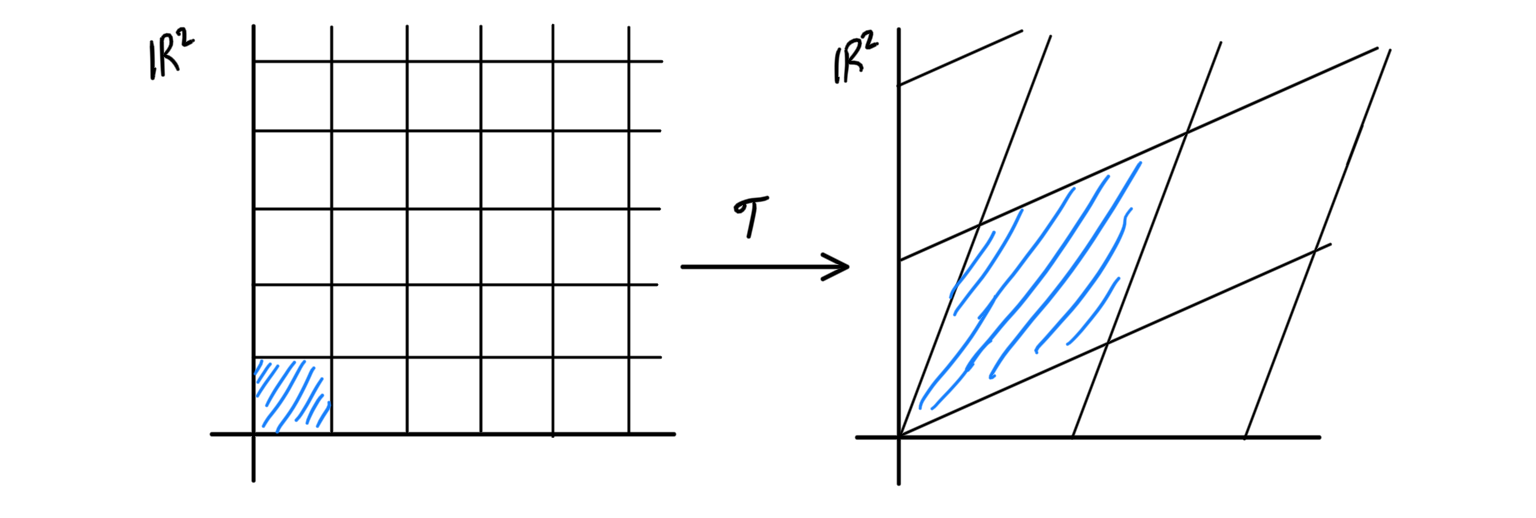
\includegraphics[scale=0.25]{img/Determinant.PNG}
  \end{center}

  \begin{proposition}
  The column vectors of $A$ are linearly dependent if and only if $\det{A} = 0$. 
  \end{proposition}
  \begin{proof}
  By linearity, it is sufficient to prove that if two column vectors $a_i$ and $a_j$ of a matrix $A$ are equal, then $\det{A} = 0$. This can be easily seen by property (ii) of determinants. 
  \end{proof}

  \begin{theorem}
  \[ \det{\bigg(\prod_i A_i \bigg)} = \prod_i \det{A_i}\]
  \end{theorem}

  \begin{theorem}
  A matrix is invertible if and only if its determinant is nonzero. 
  \end{theorem}
  \begin{proof}
  A matrix is invertible $\iff$ it is nonsingular $\iff$ its columns are linearly independent $\iff$ its determinant is nonzero, by the previous proposition. 
  \end{proof}

  \begin{corollary}
  Given $n \times n$ matrix $A$,
  \[\det{(A^{-1})} = \frac{1}{\det{A}}\]
  \end{corollary}

  \begin{theorem}
  The determinants of similar matrices are equal. 
  \end{theorem}
  \begin{proof}
  Let $A$ and $B$ be similar matrices. Then, there exists an $S$ such that $A = S^{-1} B S$ and 
  \[ \det{(A)} = \det{(S^{-1} B S} = \det{(S^{-1})} \det{(B)} \det{(S)} = \det{B}\]
  \end{proof}

  This theorem implies that the determinant is an intrinsic property of a linear transformation, so it is invariant under a change of basis. That is, choosing different matrix representations of a linear transformation does not change the determinant.  

  \begin{corollary}
  \[\det{(A)} = \det{(A^T)}\]
  \end{corollary}
  \begin{proof}
  $A$ is similar to $A^T$, which will be proven in chapter 6. 
  \end{proof}

  \begin{proposition}
  The properties of the determinant combined with the previous corollary implies that 
  \begin{enumerate}
      \item Adding a scalar multiple of a row/column to another row/column doesn't affect the determinant. 
      \item Interchanging two rows/columns switches the sign of the determinant. 
      \item Multiplying a row/column by $\alpha$ multiplies the determinant by $\alpha$. 
  \end{enumerate}
  \end{proposition}

  \begin{theorem}
  Let $A$ be an $n \times n$ matrix whose first column is $e_1$
  \[A = \begin{pmatrix}
  1&*&*&* \\
  0 &&& \\
  \ldots& & A_{11}& \\
  0&&&
  \end{pmatrix}\]
  where $A_{11}$ is the $(n-1) \times (n-1)$ submatrix of $A$ with entries $a_{i j}, \; i, j > 1$. Given this, 
  \[\det{A} = \det{A_{11}}\]
  \end{theorem}
  \begin{proof}
  Using column reduction, we can see that 
  \[ \det{A} = \det{\begin{pmatrix}
  1&0&0&0 \\
  0 &&& \\
  \ldots& & A_{11}& \\
  0&&&
  \end{pmatrix}}\]
  it is clear that the right hand side is equal to $\det{A_{11}}$ since it behaves exactly like $\det{A_{11}}$ with respect to the three properties. 
  \end{proof}

  \begin{corollary}
  Let $A$ be an upper or a lower triangular matrix. Then the determinant of $A$ is the product of its diagonal entries. That is,  
  \[ \det{A} = \prod_{i} a_{i i}\]
  \end{corollary}
  \begin{proof}
  We apply the previous theorem recursively to satisfy when $A$ is upper triangular. Since $\det{(A)} = \det{(A^T)}$, this fact can be applied to lower triangular matrices too. 
  \end{proof}

  It is once again verified that the three elementary row (and column) operations affect the determinant in the way stated in Proposition 5.5. To elaborate, since $E_1, E_2$, and $E_3$ are all lower triangular, we can compute their determinants easily
  \begin{align*}
      \det{E^1_{\alpha \times i + j}} = 1 \\
      \det{E^2_{i j}} = -1 \\
      \det{E^3_{\alpha \times i}} = \alpha
  \end{align*}
  and multiplying matrix $A$ by elementary matrices $E^1, E^2$, and $E^3$ multiplies the determinant by $1, -1$, and $\alpha$, respectively. 

  We can describe the determinant visually. Given a linear mapping $A: V \longrightarrow V$, we can fix any basis $\{e_1, e_2, ..., e_n\}$ on $V$. Note that these basis vectors do not need to be orthogonal, nor are they restricted to any magnitude. The set of vectors 
  \[\Big\{ \sum_{i=1}^n c_i e_i \; | \; 0 \leq c_i \leq 1, i = 1, 2, ..., n\Big\}\]
  forms an $n$-dimensional parallelepiped in $V$. Let the volume of this parallelepiped be $U$. Let $W$ be the volume of the parallelepiped 
  \[\Big\{ \sum_{i=1}^n c_i A e_i \; | \; 0<c_i<1, i = 1, 2, ..., n\Big\}\]
  which is formed by the transformed basis vectors $\{Ae_1, Ae_2, ..., Ae_n\}$. We can view this latter shape as the image of the first parallelepiped under transformation $A$. Then, 
  \[ \det{A} = W / V \]
  That is, the ratio of the transformed parallelepiped to the original parallelepiped is the determinant. This is consistent with the properties of the determinant. For example, if $A$ is not isomorphic, then the parallelepiped will get "squished" into a lower-dimensional parallelepiped with volume $0$. The fact that we use a ratio between the original and transformed parallelepiped allows this value to be invariant under the basis that we use. 

  Computationally, finding the LUP decomposition of a matrix $A$ is the best known algorithm to compute the determinant of a general $n \times n$ matrix. That is, 
  \[ \det{A} = \det{L} \det{U} \det{P} = \pm \det{U} = \pm \prod_i u_{i i}\]
  since $\det{L} = 1$ and $\det{P} = \pm 1$. 

  There are other methods to compute the determinant. First, we state the simple but useful formula.

  \begin{proposition}
  \[\det{\begin{pmatrix}
  a&b\\c&d 
  \end{pmatrix}} = a d - b c\] 
  \end{proposition}

  \begin{definition}
  Given an $n \times n$ matrix $A$, the $(i j)$th minor of $A$, denoted $A_{i j}$, is the determinant of the $(n-1) \times (n-1)$ matrix formed by removing the $i$th row and $j$ th column from $A$. 
  \end{definition}

  \begin{theorem}[Laplace Expansion]
  Let $A$ be an $n \times n$ matrix and $j$ any index between $1$ and $n$. Then
  \[\det{A} = \sum_i (-1)^{i + j} a_{i j} A_{i j}\]
  that is, the alternating sums of the $ij$th minors multiplied by the $ij$th entries in the $j$th column of $A$. This can be done by choosing an arbitrary $i$th row, which leads to the alternative formula 
  \[\det{A} = \sum_j (-1)^{i + j} a_{i j} A_{i j} \]
  \end{theorem}

  \begin{theorem}[Cramer's Rule]
  Given a system of linear equations in the form $A x = b$ where $A$ is an $n \times n$ matrix, the solutions of this system can be expressed with the formulas 
  \[ x_i = \frac{ \det{A_i}}{\det{A}}\]
  where $\det{A_i}$ is the matrix formed by replacing $a_i$, the $i$th column of $A$, by the column vector $b$. 
  \end{theorem}

  Albeit very computationally heavy, determinants can also be used to calculate the inverse of a matrix. 

  \begin{theorem}
  The inverse matrix $A^{-1}$ of an invertible matrix $A$ has the form 
  \[(A^{-1})_{i j} = (-1)^{i+j} \frac{\det{A_{i j}}}{\det{A}}\]
  \end{theorem}

  \begin{definition}
  The trace of a square matrix $A$, denoted $\Tr{A}$, is the sum of its diagonal entries. 
  \[\Tr(A) = \sum_{i} a_{ii}\]
  \end{definition}

  \begin{proposition}
  \[\Tr(\lambda A + \alpha B) = \lambda \Tr(A) + \alpha \Tr(B)\]
  \end{proposition}
  \begin{proof}
  Obvious if we look at the entries of $A$ and $B$ and see that it is bilinear.
  \end{proof}

  \begin{theorem}[Cyclic Property of the Trace]
  \[\Tr{\bigg(\prod_{i=1}^n A_i\bigg)} = \Tr{\bigg(A_n \prod_{i=1}^{n-1} A_i\bigg)}\]
  \end{theorem}
  \begin{proof}
  We first prove when $m=2$. Given that the subscripts $i j$ denote that $(i,j)$th element of a matrix, observe that
  \begin{align*}
      (AB)_{ij} = \sum_{k} A_{ik} B_{kj} & \implies (AB)_{ii} = \sum_{K} A_{ik} B_{ki} \\
      & \implies \Tr(AB) = \sum_{i} \sum_{k} A_{ik} B_{ki} \\
      & \;\;\;\;\;\;\;\;\;\;\;\;\;\;\;\;\;\;\;\;\;\;= \sum_{k} \sum_{i} B_{ki} B_{ik} = Tr(BA)
  \end{align*}
  Similarly, for $m=3$
  \begin{align*}
      (ABC)_{ij} = \sum_{k,l} A_{ik} B_{kl} C_{lj} & \implies \Tr(ABC) = \sum_{i,k,l} A_{ik} B_{kl} C_{li} \\ 
      & \;\;\;\;\;\;\;\;\;\;\;\;\;\;\;\;\;\;\;\;\;\;\;\;\;= \sum_{i,k,l} C_{li} A_{ik} B_{kl} = \Tr(CAB)
  \end{align*}
  And so we can generalize for $m$. 
  \end{proof}

  \begin{corollary}
  The trace is invariant under a change of basis. That is, the trace is an intrinsic property of a linear transformation since it does not change depending on how it is represented. 
  \end{corollary}
  \begin{proof}
  Given that $A$ is similar to $B$. 
  \[\Tr(B) = \Tr(S A S^{-1}) = \Tr(S^{-1} S A) = \Tr(A) \]
  \end{proof}

  \begin{theorem}
  Let $A$ be a $n \times n$ skew-symmetric matrix over $\mathbb{C}$ (or any field of characteristic $\neq 2$). If $n$ is odd, 
  \[\det{A} = 0 \]
  \end{theorem}
  \begin{proof}
  \[\det{A} = \det{A^T} = \det{-A} = (-1)^n \det{A} \implies \det{A} = 0 \]
  \end{proof}

  We can actually conclude something even futher about antisymmetric matrices. 

  \begin{theorem}
  The determinant of an antisymmetric matrix $A$ of even order is the square of a homogeneous polynomial of degree $n/2$ in the entries of $A$. That is, 
  \[\det{A} = P^2\]
  The polynomial $P$ is called the \textbf{Pfaffian}. 
  \end{theorem}

  \begin{definition}
  A \textbf{Vandermonde matrix} is a square matrix whose columns form a geometric progression. That is, let $a_1, a_2, ..., a_n$ be $n$ scalars. Then, $V(a_1, a_2, ..., a_n)$ is the $n \times n$ matrix
  \[\begin{pmatrix}
  1&1&\ldots&1&1 \\
  a_1&a_2&\ldots&a_{n-1}&a_n\\
  \vdots&\vdots&\ddots&\vdots&\vdots\\
  a_1^{n-2}&a_2^{n-2}&\ldots&a_{n-1}^{n-2}&a_n^{n-2}\\
  a_1^{n-1}&a_2^{n-1}&\ldots&a_{n-1}^{n-1}&a_n^{n-1}
  \end{pmatrix}\]
  \end{definition}

  \begin{theorem}
  The determinant of a Vandermonde matrix is
  \[\det{V(a_1, a_2, ..., a_n)} = \prod_{j>i} (a_j - a_i)\]
  \end{theorem}

  A symmetry in the multivariable expression of a determinant can also reveal a symmetry in the matrix.

  \begin{example}[2019 Putnam A1]
  The symmetric polynomial 
  \[ f(x, y, z) = x^3 + y^3 + z^3 - 3 x y z\]
  can be expressed as the determinant of the $3 \times 3$ matrix
  \[\det{\begin{pmatrix}
  x&y&z\\
  z&x&y\\
  y&z&x
  \end{pmatrix}}\]
  \end{example}

\subsection{Matrices in Block Form}

  \begin{theorem}
  Given $2 \times 2$ block matrices
  \[X = \begin{pmatrix}
  A_1&B_1\\C_1&D_1
  \end{pmatrix}, \; \; Y = \begin{pmatrix}
  A_2&B_2\\C_2&D_2
  \end{pmatrix}\]
  We can compute $X Y$ similarly to regular matrix multiplication, treating the blocks as entries. 
  \[ X Y = \begin{pmatrix}
  A_1&B_1\\C_1&D_1
  \end{pmatrix} \begin{pmatrix}
  A_2&B_2\\C_2&D_2
  \end{pmatrix} = \begin{pmatrix}
  A_1 A_2 + B_1 C_2 & A_1 B_2 + B_1 D_2 \\
  C_1 A_2 + D_1 C_2 & C_1 B_2 + D_1 D_2 
  \end{pmatrix}\]
  Furthermore, this process can be done in general for any $m \times n$ block matrix $X$ and $n \times p$ block matrix $Y$. 
  \end{theorem}

  \begin{theorem}
  Given that $I_N, A, B$ are $n \times n$ matrices, define the $(2n) \times (2n)$ matrix 
  \[X = \begin{pmatrix}
  I & 0 \\ A & B
  \end{pmatrix}\]
  Then 
  \[\det{X} = \det{B}\]
  \end{theorem}
  \begin{proof}
  We can perform Gauss elimination to reduce $X$ without affecting the determinant.
  \[\det{\begin{pmatrix}
  I&0\\A&B
  \end{pmatrix}} = \det{
  \begin{pmatrix}
  I&0\\
  0&B
  \end{pmatrix}} = \det{B}\]
  since it satisfies the correct properties for $\det{B}$. 
  \end{proof}

  \begin{corollary}
  \[\det{\begin{pmatrix}
  A&0\\C&D
  \end{pmatrix}} = \det{A} \det{D}\]
  \end{corollary}

  \begin{proof}
  \[ \det{\begin{pmatrix}
  A&0\\C&D 
  \end{pmatrix}} = \det{\begin{pmatrix}
  A&0\\C&I
  \end{pmatrix} \begin{pmatrix}
  I&0\\0&D
  \end{pmatrix}} = \det{\begin{pmatrix}
  A&0\\C&I
  \end{pmatrix}} \det{\begin{pmatrix}
  I&0\\0&D
  \end{pmatrix}}\]
  \end{proof}

  However, 
  \[\det{\begin{pmatrix}
  A&B\\C&D
  \end{pmatrix}} \neq \det{A} \det{D} - \det{B} \det{C}\]

  Rather, we introduce the following theorem

  \begin{theorem}
  \begin{align}
      \det{\begin{pmatrix} A&B\\C&D \end{pmatrix}}  & = \det{(A)} \det{(D - C A^{-1} B)} \\
      & = \det{(D)} \det{(A - B D^{-1} C)}
  \end{align}
  \end{theorem}
  \begin{proof}
  \[\begin{pmatrix} A&B\\C&D\end{pmatrix} = \begin{pmatrix}
  A&0\\C&I\end{pmatrix} \begin{pmatrix}
  I& A^{-1} B \\ 0 & D - C A^{-1} B
  \end{pmatrix}\]
  by similarity, equation $(6)$ is equal to equation $(7)$. 
  \end{proof}

  \begin{definition}
  A \textbf{block diagonal matrix} is a square matrix in block form such that the diagonal blocks are square matrices and all off-diagonal blocks are zero matrices. 
  \[A = \begin{pmatrix}
  A_1&0&\ldots&0\\
  0&A_2&\ldots&0\\
  \vdots&\vdots&\ddots&\vdots\\
  0&0&\ldots&A_k
  \end{pmatrix}\]
  \end{definition}

  \begin{theorem}
  Given a matrix $A$ in block diagonal form, with diagonal blocks $A_1, A_2, ..., A_k$,
  \[\det{A} = \prod_{i=1}^k A_i, \; \; \Tr{A} = \sum_{i=1}^k \Tr{A_i}\]
  Furthermore, $A$ is invertible if and only if all the $A_i$'s are invertible, and 
  \[A^{-1} = \begin{pmatrix}
  A_1&0&\ldots&0\\
  0&A_2&\ldots&0\\
  \vdots&\vdots&\ddots&\vdots\\
  0&0&\ldots&A_k
  \end{pmatrix} = \begin{pmatrix}
  A_1^{-1}&0&\ldots&0\\
  0&A_2^{-1}&\ldots&0\\
  \vdots&\vdots&\ddots&\vdots\\
  0&0&\ldots&A_k^{-1}
  \end{pmatrix}\]
  \end{theorem}
  \begin{proof}
  The results are obvious when performing block multiplication or Gauss Elimination. 
  \end{proof}

\subsection{Dodgson Condensation}

  We already know that the LUP decomposition is an algorithm used to compute the determinant of a general $n \times n$ matrix. We will introduce another, called \textbf{Dodgson condensation}. The algorithm can be described in the following steps.

  \begin{enumerate}
      \item Let $A$ be a given $n \times n$ matrix. Arrange $A$ so that no zeros occur in its interior (this can be done by any combination of elementary row or column operations that would not change the determinant). 
      \item Create an $(n-1) \times (n-1)$ matrix $B$ consisting of the determinants of every $2 \times 2$ submatrix of $A$. Explicitly, 
      \[B = \det{\begin{pmatrix}
      a_{i,j} & a_{i,j+1} \\ a_{i+1,j} & a_{i+1,j+1}
      \end{pmatrix}}\]
      \item With this $(n-1) \times (n-1)$ matrix $B$, perform step $2$ to obtain an $(n-2) \times (n-2)$ matrix $C$. Divide each term in $C$ by the corresponding term in the interior of $A$. 
      \[C_{i,j} = \det{\begin{pmatrix}
      b_{i,j} & b_{i,j+1} \\ b_{i+1,j} & b_{i+1,j+1}
      \end{pmatrix}} \bigg/ a_{i+1,j+1}\]
      \item Let $A = B$ and $B=C$. Repeat step $3$ as necessary until the $1 \times 1$ matrix is found, which is the determinant. 
  \end{enumerate}

  The reason that we do not want $0$s in $A$ is because then in doing step $3$ we may divide by $0$. 

  \begin{example}
  Let us find
  \[\det{\begin{pmatrix}
  -2&-1&-1&-4\\-1&-2&-1&-6\\-1&-1&2&4\\2&1&-3&-8
  \end{pmatrix}}\]
  All of the interior elements are nonzero, so there is no need to rearrange the matrix. We calculate
  \[\begin{pmatrix}
  -2&-1&-1&-4\\-1&-2&-1&-6\\-1&-1&2&4\\2&1&-3&-8
  \end{pmatrix} \rightarrow \begin{pmatrix}
  3&-1&2\\-1&-5&8\\1&1&-4
  \end{pmatrix} \rightarrow \begin{pmatrix}
  -16&2\\4&12
  \end{pmatrix}\]
  With this $2 \times 2$ matrix, we must divide each term by the interior of the original $A$. 
  \[\begin{pmatrix}
  -16/-2 & 2/-1\\4/-1 & 12/2
  \end{pmatrix} = \begin{pmatrix}
  8&-2\\-4&6
  \end{pmatrix}\]
  Calculating this determinant gives $40$, and dividing by the interior of the $3 \times 3$ matrix $(-5)$ gives $\det{A} = 40/-5 = -8$. 
  \end{example}

\subsection{Matrix Calculus}

  There is nothing special about matrix calculus on its own, since matrices are themselves vectors; they can be sufficiently analyzed using vector calculus. Regardless, we will emphasize a few points. Let
  \[A: \mathbb{R} \longrightarrow \text{Mat}(m \times n, \mathbb{R})\]
  be a matrix valued differential function. That is, the $m \times n$ component functions of $A$ is differentiable. Then, just like in calculus, we introduce differentiation rules.
  \begin{align*}
      & \frac{d}{d x} \big( A(t) + B(t)\big) = \frac{d}{d t} A(t) + \frac{d}{d t} B(t) \\
      & \frac{d}{d x} \big( c A(t)\big) = c \frac{d}{d t} A(t)
  \end{align*}
  The scalar multiplication can actually be extended. By linearity (of matrix multiplication), we can say that if $A$ is independent of $t$, then 
  \[\frac{d}{d x} A B (x) = A \frac{d}{d x} B(x)\]
  The linearity of the derivative allows us to state more rules. Given that $v: \mathbb{R}^n \longrightarrow \mathbb{R}$ is a scalar valued function and $l \in (\mathbb{R}^n)^*$, then  
  \[\frac{d}{d x} l \big( v(x) \big) = l \bigg( \frac{d}{d x} v(x) \bigg)\]
  This result can be extended to when $v$ is replaced by matrix valued function $A$ and $l$ is replaced by $\phi: \text{Mat}(m \times n, \mathbb{R}) \longrightarrow \mathbb{R}$. 
  \[\frac{d}{d x} \phi \big( A(x) \big) = \phi \bigg( \frac{d}{d x} A(x) \bigg)\]
  Since the trace is a linear operator, we have the following theorem. 

  \begin{theorem}
  Given a linear function $A: \mathbb{R} \longrightarrow \text{Mat}(n, \mathbb{R})$ with paramater $x$, 
  \[\frac{d}{d x} \Tr{A} = \Tr \bigg( \frac{d}{d x} A \bigg)\]
  Note that $A$ in here really means $A(x)$.
  \end{theorem}

  The product rule of matrix calculus is similar.
  \[\frac{d}{d x} A B = \bigg(\frac{d}{d x} A\bigg) \cdot B + A \cdot \bigg(\frac{d}{d x} B \bigg)\]
  It is also noting that the derivative of the inner product of two vector valued functions $v, w: \mathbb{R} \longrightarrow \mathbb{R}^n$ is 
  \[\frac{d}{d x} \big( v(x), w(x) \big) = \Big( \frac{d}{d x} v(x), w(x) \Big) + \Big( v(x), \frac{d}{d x} w(x) \Big)\]

  \begin{definition}
  A matrix valued function $A$ is \textbf{invertible at a point $x \in \mathbb{R}$} if there exists a function, denoted $A^{-1}$ such that
  \[A(x) A^{-1} (x) = A^{-1}(x) A(x) = I\]
  where $I$ is the identity matrix. If there exists such $A^{-1}$ for all values $x \in \mathbb{R}$, then $A$ is said to be \textbf{invertible}. 
  \end{definition}

  \begin{theorem}
  Let $A$ be a matrix valued function, differentiable and invertible. Then, the function $A^{-1}$ is also differentiable and 
  \[\frac{d}{d x} A^{-1} = - A^{-1} \bigg( \frac{d}{d x} A \bigg) A^{-1}\]
  \end{theorem}
  \begin{proof}
  We derive this using the product rule. 
  \begin{align*}
      0 = \frac{d}{d x} I & = \frac{d}{d x} \big( A(x) A^{-1} (x) \big) \\
      & = A(x) \bigg(\frac{d}{d x} A^{-1} (x) \bigg) + \bigg( \frac{d}{d x} A(x) \bigg) A^{-1} (x) \\
      \implies \frac{d}{d x} A^{-1} (x) & = - A^{-1} (x) \bigg( \frac{d}{d x} A(x) \bigg) A^{-1}(x)
  \end{align*}
  \end{proof}
  Note that the chain rule is a rule of differentiaion that applies for scalar valued functions. That is, given $f: V \longrightarrow \mathbb{R}$ and $g: \mathbb{R} \longrightarrow V$ ($V$ vector space), 
  \[\frac{d}{d x} f \circ g (x) = f^\prime \big( g(x) \big) \cdot \frac{d}{d x} g(x)\]
  The $\cdot$ operation in the right hand side is the operation of multiplication in the field $\mathbb{R}$. But given $f: \text{Mat}(n, \mathbb{R}) \longrightarrow \mathbb{R}$ and $A \mathbb{R} \longrightarrow \text{Mat}(n, \mathbb{R})$, multiplication within the algebra of matrices are inherently different than component-wise operations, so the chain rule does not apply (it would apply if matrix multiplication was defined component-wise). 

  \begin{example}
  Let $f(A) \equiv A^2$, and let $A$ be a matrix valued function. Then, 
  \begin{align*}
      \frac{d}{d x} f \circ A(x) = \frac{d}{d x} \big( A(t) \big)^2 & = \bigg( \frac{d}{d x} A(x) \bigg) \cdot A(x) + A(x) \cdot \bigg( \frac{d}{d x} A(x) \bigg) \\
      & \neq 2 A(x) \cdot \frac{d}{d x} A(x)
  \end{align*}
  since matrix multiplication is in general not commutative. 
  \end{example}

  \begin{proposition}
  \[\frac{d}{d x} A^k = A^\prime A^{k-1} + A A^\prime A^{k-2} + ... + A^{k-2} A^\prime A + A^{k-1} A^\prime\]
  \end{proposition}
  \begin{proof}
  We inductively apply the product rule
  \[\frac{d}{d x} A^k = A^\prime A^{k-1} + A \frac{d}{d x} A^{k-1}\]
  \end{proof}

  \begin{corollary}
  Given any polynomial $p$ with $A$ a differentiable, square matrix valued function, if $A$ and $A^\prime$ commute, then 
  \[\frac{d}{d x} p(A) = p^\prime (A) A^\prime\]
  \end{corollary}
  \begin{proof}
  We can completely define differentiation over the vector space of polynomials with the formula
  \[\frac{d}{d x} A^k = k A^{k-1} A^\prime \; \forall k \in \mathbb{N}\]
  \end{proof}

  \begin{corollary}
  Given polynomial $p$ with $A$ a differentiable, square matrix valued function, 
  \[\frac{d}{d x} \Tr{p(A)} = \Tr{\big( p^\prime(A) \cdot A^\prime \big)}\]
  \end{corollary}
  \begin{proof}
  Use the cyclic trace property.
  \end{proof}

  \begin{definition}
  The \textbf{exponential map} is defined
  \[\text{exp}: \text{Mat}(n, \mathbb{C}) \longrightarrow \text{Mat}(n, \mathbb{C})\]
  where 
  \[e^A = I + A + \frac{1}{2!} A^2 + \frac{1}{3!} A^3 + ... = \sum_{k=0}^\infty \frac{1}{k!} A^k\]
  where $A^0 \equiv I$. This can clearly be extended to when $A$ is a square, matrix valued function. 
  \end{definition}

  This final theorem establishes the connection between the determinant and trace. 

  \begin{theorem}
  Given a differentiable square matrix valued function $A$ such that $A$ is invertible for a certain $x \in \mathbb{R}$, then 
  \[\frac{d}{d x} \log{\det{A}} = \Tr \bigg( A^{-1} \frac{d}{d x} A \bigg)\]
  Where the log mapping is the inverse of the exponential mapping of matrices. 
  \end{theorem}

  \begin{definition}
  The \textbf{commutator} in the algebra of $n \times n$ matrices is defined as 
  \[[A, B] = A B - B A\]
  \end{definition}

  \begin{theorem}
  If $A$ and $B$ are commuting square matrices, then 
  \[e^{A + B} = e^A \, e^B\]
  In general, the solution $C$ to the equation
  \[e^{A} \, e^B = e^C\]
  is given by the \textbf{Baker-Campbell-Hausdorff formula}, defined
  \[C = A + B + \frac{1}{2}[A,B] + \frac{1}{12} [A,[A,B]] - \frac{1}{12} [B,[A,B]] + ...\]
  consisting of terms involving higher commutators of $A$ and $B$. The full series is much too complicated to write, so we ask the reader to be satisfied with what is shown. 
  \end{theorem}

  \begin{corollary}
  \[\Tr{\log{e^A \, e^B}} = \Tr{A} + \Tr{B}\]
  \end{corollary}


\section{Spectral Theory} 

\subsection{Spectral Theory of General Mappings}

  \begin{definition}
  Let $A: V \longrightarrow V$ be a linear transformation over $\mathbb{F}$. If there exists a vector $v \in V$ such that
  \[ A v = \lambda v, \; \lambda \in \mathbb{F}\]
  then $a$ is called an \textbf{eigenvalue} of $A$, and $v$ is an \textbf{eigenvector} of $A$. Clearly, if a basis is realized for $V$ and $A$ is represented as a matrix, $v$ would have a basis representation. However, the value of $\lambda$ is invariant. The set of all eigenvalues 
  \[\lambda(A) \equiv \{ \lambda_1, \lambda_2, ..., \lambda_k\}\]
  is called the \textbf{spectrum} of $A$. 
  \end{definition}

  For a given eigenvalue $\lambda$ and its corresponding eigenvector $v$, it is clear that by linearity, every vector in $\Span v$ is an eigenvector, too. 

  Now that we have defined eigenvalues and eigenvectors, we first provide a visual description of these terms. Given a linear transformation $A: V \longrightarrow V$, we can visualize a certain basis of $V$ such that all the linear transformation $A$ does on that basis is merely extend or contract the basis vectors.

  \begin{definition}
  Given a $n \times n$ matrix $A$, the \textbf{characteristic polynomial} of $A$, denoted $p_A (t)$, is defined
  \[ p_A (t) \equiv \det{(A - t I)}\]
  The mapping $A \mapsto p_A (t)$ can be thought of as a mapping from Mat$(n, \mathbb{F}) \longrightarrow \mathbb{F}[t]$, where Mat$(n, \mathbb{F})$ is the algebra of $n \times n$ matrices over field $\mathbb{F}$, and $\mathbb{F}[t]$ is the polynomial algebra over $\mathbb{F}$. $p_A (t)$ is invariant under matrix similarity. 
  \end{definition}

  The motivation for defining such a polynomial is that it allows us to compute the eigenvalues of $A$. 
  \begin{definition}
  The \textbf{characteristic equation} of $A$ is defined by equating $p_A (t) = 0$. 
  \end{definition}

  \begin{proposition}
  The solutions of the characteristic equation of $A$ (i.e. the roots of $p_A (t)$) is precisely the spectrum of $A$. 
  \end{proposition}

  \begin{proof} $(\rightarrow)$ Let there be a $t = \lambda$ such that $p_A (\lambda) = 0 \iff \det{(A - \lambda I)} = 0$ which is equivalent to saying that ker$(A - \lambda I)$ is nontrivial. There must exist a $v \in $ ker$(A - \lambda I)$, meaning that $(A - \lambda I) v = 0 \iff A v = \lambda v$. By definition, $\lambda$ is an eigenvalue of $A$. \\
  $(\leftarrow)$ This reasoning can be extended in the opposite direction. 
  \end{proof}

  \begin{theorem}
  Eigenvectors of a linear transformation $A$ corresponding to different eigenvalues are linearly independent, but not necessarily orthogonal. It follows that if the characteristic polynomial of a $n \times n$ matrix $A$ has $n$ distinct roots, then $A$ has $n$ linearly independent eigenvectors. 
  \end{theorem}

  \begin{proof}
  Simple, by contradiction.
  \end{proof}

  \begin{example}
  It is clear that the Fibonacci sequence can be produced with matrix multiplication as such 
  \[ \begin{pmatrix}
  a_{n+1} \\ a_n
  \end{pmatrix} = A^n \begin{pmatrix}
  a_1 \\ a_0
  \end{pmatrix} = \begin{pmatrix}
  1&1\\1&0
  \end{pmatrix}^n \begin{pmatrix}
  1\\1
  \end{pmatrix}\]
  Given that 
  \[\lambda_1 = \frac{1+\sqrt{5}}{2}, \; \lambda_2 = \frac{1 - \sqrt{5}}{2}\]
  we can diagonalize $A$ into the form 
  \[A = \begin{pmatrix}
  \frac{1}{\lambda_1 - \lambda_2} & \frac{\lambda_2}{\lambda_2 - \lambda_1} \\
  \frac{1}{\lambda_2 - \lambda_1} & \frac{\lambda_1}{\lambda_1 - \lambda_2}
  \end{pmatrix} \begin{pmatrix}
  \lambda_1 & 0 \\ 0 & \lambda_2 
  \end{pmatrix} \begin{pmatrix}
  \lambda_1 & \lambda_2 \\
  1 & 1
  \end{pmatrix} \implies A^n = S^{-1} \begin{pmatrix}
  \lambda_1^n & 0 \\ 0 & \lambda_2^n 
  \end{pmatrix} S\]
  which implies that after evaluating, we get 
  \[ a_n = \frac{1}{\sqrt{5}} \bigg( \Big(\frac{1+\sqrt{5}}{2}\Big)^n - \Big(\frac{1-\sqrt{5}}{2}\Big)^n \bigg)\]
  This is a surprising result since it also says that the expression above is always an integer for all natural number $n$. 
  \end{example}
  \begin{definition}
  Given a subspace $U_1 \subset U$ and linear transformation $T: U \longrightarrow U$. We say that $U_1$ is \textbf{invariant} under $T$ if 
  \[u \in U_1 \implies T u \in U_1\]
  \end{definition}

  \begin{theorem} 
  Let $a_1, a_2, ..., a_n$ be the eigenvalues of $A$. Then 
  \[\sum_i a_i = \Tr{A}, \;\;\; \prod_i a_i = \det{A}\]
  \end{theorem}

  \begin{proof}
  The mapping $A \mapsto \det{(A - x I)}$ is a mapping from the set of $n \times n$ matrices to the polynomial algebra $\mathbb{F}[x]$. Direct application of the Viete's formulas in $\mathbb{F}[x]$ produces the statement and this result can be extended to the rest of the formulas. 
  \end{proof}

  \begin{theorem}[Spectral Mapping Theorem]
  Let $q$ be any polynomial, $A$ a square matrix with an eigenvalue $a$. Then: 

  i) $q(a)$ is an eigenvalue of $q(A)$. 

  ii) Every eigenvalue $q(A)$ is of the form $q(a)$, where $a$ is an eigenvalue of $A$. 
  \end{theorem}
  \begin{proof} 
  i) Let $h$ be an eigenvector of A with corresponding eigenvalue $a$. 
  \begin{align*}
      Ah = ah & \implies A^{2} h = Aah = aAh = a^{2} h \\
   & \implies A^{n} h = a^{n} h   \\
   & \implies q(A)h = q(a)h \\
   & \implies q(a) \text{ is an eigenvalue of }q(A)
  \end{align*}
  ii) Let $p$ be the eigenvalue of $q(A) \iff \det{\big(q(A) - p I\big)} = 0$. We expand: 
  $$ q(s) - p = c\prod \big(s-r_{i}\big), r_{i} \in \mathbb{C} $$ 
  Replacing the variable $s$ with $A$, we have
  $$ q(A) - pI = c \prod \big(A-r_{i}I\big) $$
  Since $\det{\big( q(A) - pI\big)} = 0$, at least one $r_{i}$, say $r_{k}$ exists such that $\det{\big( A - r_{k} I \big)} = 0 \iff r_{k}$ is an eigenvalue of $A$. Since $q(r_{j})-p = 0$, $p = q(r_{j})$ is an eigenvalue of $q(A)$. 
  \end{proof}

  The following theorem is an equivalent version of the spectral mapping theorem.
  \begin{theorem}
  Let $A$ be a $n \times n$ matrix and let $f$ be a polynomial. If the chracteristic polynomial of $A$ has factorization 
  \[p_A (t) = \prod_{i = 1}^n (t - \lambda_i)\]
  then the characteristic polynomial of the matrix $f(A)$ is given by 
  \[p_{f(a)} (t) = \prod_{i = 1}^n (t - f(\lambda_i))\]
  \end{theorem}

  We can actually create a bound on the spectrum of a square matrix. 

  \begin{theorem}[Gershgorin Circle Theorem]
  Let $A \in $ Mat$(n, \mathbb{C})$ with entries $a_{i j}$. Let $R_i = \sum_{i \neq j} |a_{i j}|$ be the sum of the absolute values of the non-diagonal entries of the $i$th row, and let $D_(a_{i i}, R_i) \subset \mathbb{C}$ be a closed disk with radius $R_i$ centered at $a_{i i}$ in the complex plane, called a \textbf{Gershgorin Disk}. Then every eigenvalue of $A$ lies within the union of all $n$ Gershgorin Disks. That is, 
  \[ \lambda_j (A) \in \bigcup_{i= 1}^{n} D_(a_{i i}, R_i) \subset \mathbb{C}, \text{ for all } j\]
  \end{theorem}

  \begin{proof}
  Let $\lambda$ be an eigenvalue of $A$ with its eigenvector $v = (v_j)$. Scale $v$ by multiplying it by $ \pm 1 / \max{\{|v_j|\}_j}$ to get a vector $x$ with its maximal entry $x_i = 1$ and $|x_j| \leq 1, \; j \neq i$. Then, 
  \[A x = \lambda x \implies \sum_{j} a_{i j} x_j = \lambda x_i = \lambda \implies \sum_{j \neq i} a_{i j} x_j + a_{i i} = \lambda\]
  Applying the triangle inequality, 
  \[| \lambda - a_{i i} | = \bigg| \sum_{j \neq i} a_{i j} x_j\bigg| \leq \sum_{j \neq i} |a_{i j}| |x_j| \leq \sum_{j \neq i} |a_{i j}| = R_i\]
  \end{proof}

  \begin{corollary}
  The eigenvalues of $A$ must also lie within the Gershgorin discs $C_j$ corresponding to the columns of $A$. 
  \end{corollary}

  \begin{proof}
  This is a direct result from the fact that $A$ is similar to $A^T$. Alternatively, we can apply the same process in the proof above to $A^T$.
  \end{proof} 

  If one observes that the off-diagonal entries of $A$ are small in absolute value, it can be concluded that the diagonal entries are "close" to the true eigenvalues of $A$. $A$ is diagonal if and only if the Gershgorin disks are points. 

  \begin{theorem}[Cayley Hamilton]
  Every matrix $A$ satisfies its own characteristic equation. That is, 
  \[ p_{A}(A) = 0\]\
  \end{theorem} 

\subsection{Eigendecompositions and Jordan Normal Form}

  However, the entire concept of matrices are not fully grasped with just eigenvectors. If it were, then linear algebra would be a much simpler matter. To extend our toolkit, we must introduce generalized eigenvectors. From here, we will assume that our field is over $\mathbb{C}$. We use the fact that the field is over $\mathbb{C}$ because it allows us to claim that the characteristic polynomial in $\mathbb{C}[t]$ can be factored into linear components, by the fundamental theorem of algebra. 

  \begin{definition}
  A genuine eigenvector of $A$ satisfies $(A-aI)h = 0$. A \textbf{generalized eigenvector} $f$ satisfies $(A-a I)^{d} f = 0$ for some $d \geq 1$. 
  \end{definition}

  To provide a visual intuition of how generalized eigenvectors transform under $A$, observe that 
  \begin{align}
      (A - aI) h = 0 \text{ and } (A - aI)^2 f = 0 & \implies (A - aI)^f = h \\
      & \implies A f = a f + h, \; Ah = ah \\
      & \implies A^2 f = a A f + A h = a^2 f + 2 a h \\
      & \implies A^N f = A^N f + N a^{N-1} h 
  \end{align}
  This implies that the generalized eigenvector is first scaled by a factor of $a$, similar to a genuine eigenvector, but then a factor of the genuine eigenvector is then added to the scaled generalized one. Note that in higher dimensions of $N$, a greater multiple of $h$ must be added after scaling $f$. 

  This means that given an eigenvalue $\lambda$, there is always at least one genuine eigenvalue associated with $\lambda$. Furthermore, there may be additional generalized eigenvectors also corresponding to $\lambda$. This leads to the following definition

  \begin{definition}
  The subspace formed by the span of the generalized (and genuine) eigenvectors of $\lambda$ form what is called the \textbf{eigenspace associated with $\lambda$}, denoted $E(\lambda)$. 
  \end{definition}

  We can measure the characteristics of the eigenspaces with the following definitions. 

  \begin{definition}
  The \textbf{algebraic multiplicity} of an eigenvalue $\lambda$ is the dimension of its eigenspace. It is precisely
  \[\dim{E(\lambda)}\]  
  In order to compute the algebraic multiplicity of $\lambda_i$ in $A$, we find the maximal value of $d_i$ such that $(t-\lambda)^{d_i}$ divides $p_A (t)$. With this, we can define 
  \[E(\lambda) = \ker{(A - \lambda_i I)^{d_i}}\]
  \end{definition} 

  \begin{theorem}
  Given $A: V \longrightarrow V$ with eigenspaces $E(\lambda_1), E(\lambda_2), ..., E(\lambda_k)$, 
  \[E(\lambda_1) \oplus E(\lambda_2) \oplus ... \oplus E(\lambda_k) = V\]
  That is, every vector $v \in V$ can be uniquely expressed as the sum 
  \[ v = h_1 + h_2 + ... + h_k, \; h_i \in E(\lambda_i)\]
  this is called the \textbf{eigenbasis of $V$}. 
  \end{theorem}
  \begin{proof}
  The definition of algebraic multiplicity implies that each eigenspace is disjoint except at $0$ and that their dimensions sum to $\dim{V}$. 
  \end{proof}

  \begin{definition}
  The \textbf{geometric multiplicity} of an eigenvalue $\lambda$ of a linear transformation $A$ is the dimension of the span of genuine eigenvectors in its eigenspace. It is precisely 
  \[\dim{\ker{(A - \lambda I)}}\]
  Note that since the span of genuine eigenvectors is a subspace of $E(\lambda)$, the geometric multiplicity is always less than or equal to the algebraic multiplicity. 
  \end{definition}

  Now we are ready to introduce the eigendecomposition of a linear mapping $A$.

  \begin{theorem}
  Given a linear mapping $A$ with its eigenvalues $\lambda_1, \ldots, \lambda_k$ and associated eigenspaces $E(\lambda_1), \ldots, E(\lambda_k)$, $A$ maps each eigenspace to itself. That is, 
  \[A\big( E(\lambda_i) \big) \subset E(\lambda_i), \; i = 1, 2, ..., k\]
  \end{theorem}

  \begin{corollary}[Jordan Normal Form]
  Every linear mapping $A: V \longrightarrow V$ can be decomposed into the sum of the linear mappings of each eigenspace $E(\lambda_i)$. That is, it can be expressed in the form 
  \[A: \prod_i E(\lambda_i) \longrightarrow \prod_i E(\lambda_i)\]
  which we can define, given $h_i \in E(\lambda_i)$, 
  \[A(v) = A\bigg(\sum_i h_i \bigg) = \sum_i A(h_i), \; A(h_i) \in E(\lambda_i) \]
  \end{corollary}

  The process of eigendecomposition for a linear mapping $A$ is really just a clever change of basis for the $n \times n$ matrix representation of $A$ over $\mathbb{C}$, where the new basis is now the set of genuine and generalized eigenvectors. The new matrix formed by performing the change of basis on matrix $A$ is called the \textbf{Jordan Normal Form}, or \textbf{Jordan Canonical Form}, of $A$. We will now describe the construction of the JNF of an arbitrary $n \times n$ matrix. 

  It is actually simple. Let the eigenvalues of the matrix $A$ be $\lambda_1, \lambda_2, ..., \lambda_k$, with its associated eigenspaces $E(\lambda_i)$. Let the algebraic multiplicity of eigenspace $E(\lambda_i)$ be $alg_i$. Then, every $n \times n$ matrix over $\mathbb{C}$ has the block form 
  \[ J = \begin{pmatrix}
  A_1&0&0&0\\
  0&A_2&0&0\\
  0&0&...&0\\
  0&0&0&A_k
  \end{pmatrix}\]
  where each block $A_i$ represents the transformation in $E(\lambda_i)$. This means that each $A_i$ must be an $alg_i \times alg_i$ submatrix. The definition of the generalized eigenvectors shown in equation $(11)$ shows that each block must be of form 
  \[A_i = \begin{pmatrix}
  \lambda_i & 1 & 0 & ... & 0\\
  0 &\lambda_i & 1 &...&0 \\
  0&0&\lambda_i&...&0\\
  ...&...&...&...&1\\
  0&0&...&0&\lambda_i
  \end{pmatrix}\]
  With $\lambda_i$'s in the main diagonal and $1$'s in the superdiagonal of $A_i$. The first column of $A$ refers to the transformation of the genuine eigenvector, while the other columns refers to the transformation of the generalized eigenvectors, where $\lambda_i$ refers to the scaling of the $d$th generalized eigenvector and the $1$ refers to the adding of the $(d-1)$th generalized eigenvector to the scaled $d$th vector. If there are no generalized eigenvectors in an eigenspace $E(\lambda_i)$, then $A_i$ is a $1 \times 1$ matrix $( \lambda_i )$. Observe that this form is consistent with our previous theorems, especially the fact that $A$ maps distinct eigenspaces to themselves. 

  Finally, the change of basis is represented through the matrix multiplication. 
  \[J = P^{-1} A P, \; P = \begin{pmatrix}
  |&|&|&| \\ 
  f_1&f_2&...&f_n \\
  |&|&|&|
  \end{pmatrix} \]
  where $f_i$ is the genuine/generalized eigenvectors corresponding to the transformation represented in the $i$th column of $J$. The Jordan Normal Form of a matrix is unique up to the permutations of its diagonal blocks. 

  Notice that the Jordan Normal Form must be an $n \times n$ matrices over $\mathbb{C}$, not $\mathbb{R}$. However, given a matrix $A$ over $\mathbb{R}$, we can construct a similar block diagonal form over $\mathbb{R}$. Since $A$ is real $\implies p_A (t) \in \mathbb{R}[t]$, $\mu \in \mathbb{C}$ is a root of $p_A$ implies that $\bar{\mu}$ is also a root. This means that in the case where $\mu = a \pm b i$ is a pair of complex eigenvectors with eigenvectors $z$ and $\bar{z}$. The associated $2 \times 2$ Jordan block will be of form
  \[\begin{pmatrix}
  a&-b\\ b&a
  \end{pmatrix}\]
  with the associated column vectors in $P$ being
  \[v_1 = \frac{z + \bar{z}}{2}, \; v_2 = \frac{i (z - \bar{z})}{2}\]
  Notice that $z \in \mathbb{C}^n$ is a complex eigenvector belonging to complex eigenvalue $\mu$, and we make the best "approximations" of $z, \bar{z}$ and $\mu, \bar{\mu}$ with the new real vectors $v_1$ and $v_2$. Note that the Jordan block states that
  \[A(v_1) = a v_1 + b v_2, \; A(v_2) = -b v_1 + a v_2\]
  which is true since 
  \begin{align*}
      A(v_1) = A\Big( \frac{z + \bar{z}}{2} \Big) & = \frac{1}{2} \big( A(z) + A(\bar{z}) \big) \\
      & = \frac{1}{2}\big( (a+bi)z + (a-bi) \bar{z} \big) \\
      & = \frac{1}{2} \big( (a)(z + \bar{z}) + (bi) (z - \bar{z})\big) \\
      & = a \frac{z + \bar{z}}{2} + b \frac{i(z-\bar{z}}{2} = a v_1 + b v_2 \\
  \end{align*}
  and 
  \begin{align*}
      A(v_2) = A \Big( \frac{i(z-\bar{z})}{2} \Big) & = \frac{i}{2} \big( A(z) - A(\bar{z}) \big) \\
      & = \frac{i}{2} \big( (a+bi) z - (a-bi) \bar{z}\big) \\
      & = \frac{i}{2} \big( (a) (z - \bar{z}) + (bi)(z+\bar{z})\big) \\
      & = a \frac{i(z-\bar{z})}{2} - b \frac{z + \bar{z}}{2} = a v_2 - b v_1
  \end{align*}
  It suffices to only modify this case for $2 \times 2$ blocks because all complex eigenvalues of real matrices must come in conjugate pairs (but this is not necessarily true for complex matrices, which have characteristic polynomials in $\mathbb{C}[t]$). 

  \begin{corollary}
  The following $2 \times 2$ Jordan block of the form shown below can be turned into the complex Jordan block and vice versa. 
  \[\begin{pmatrix}
  \cos{\theta} & -\sin{\theta} \\
  \sin{\theta} & \cos{\theta} 
  \end{pmatrix} \xleftrightarrow{} \begin{pmatrix}
  e^{i \theta} & 0 \\
  0 & e^{- i \theta}
  \end{pmatrix}\]
  \end{corollary}

  However, there could be bigger Jordan blocks of generalized eigenspaces corresponding to conjugate pairs. Observe the following JNF, with columns (from left to right) corresponding to the transformations $h_1$ (genuine), $k_1$ (generalized), $h_2$ (genuine), and $k_2$ generalized). 
  \[\begin{pmatrix}
  e^{i \theta} & 1 & & \\
  & e^{i \theta} & & \\
  & & e^{-i \theta} & 1 \\
  & & & e^{i- \theta}
  \end{pmatrix}\]
  Using the corollary shown above, we can modify the eigenvalues and eigenvectors into real values and construct the simplest "real form" (assuming $i \neq 0, \pi$) of the matrix 
  \[\begin{pmatrix}
  \cos{\theta} & - \sin{\theta} & 1 & 0 \\
  \sin{\theta} & \cos{\theta} & 0 & 1 \\
  0 & 0 & \cos{\theta} & - \sin{\theta} \\
  0 & 0 & \sin{\theta} & \cos{\theta}
  \end{pmatrix}\]
  where the columns (from left left to right) now correspond to transformation of real eigenvectors
  \[\frac{h_1 + h_2}{2}, \frac{i(h_1 - h_2)}{2}, \frac{k_1 + k_2}{2}, \frac{i(k_1 - k_2)}{2}\]
  Therefore, we can state that the linear transformation represented by the two matrices in their respective bases are equivalent. 

  \begin{example}
  The linear operator that rotates around a vector $v$ by an angle $\theta$ has an eigendecomposition of the span of $v$ as shown (with eigenvalue $1$) and the 2-dimensional plane (having two complex eigenvalues). 
  \begin{center}
      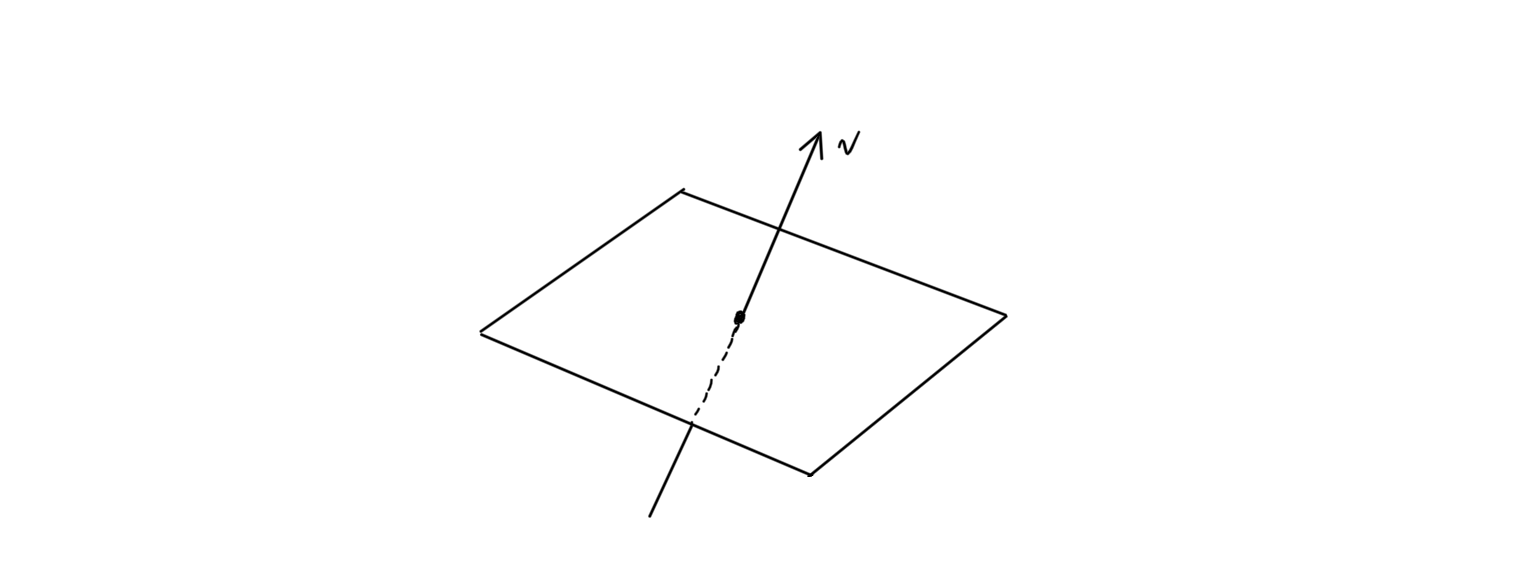
\includegraphics[scale=0.25]{img/Rotation_Map_Eigendecomposition.PNG}
  \end{center}
  \end{example}

  \begin{definition}
  A matrix is \textbf{diagonalizable} if we can perform a change of basis on it to create a diagonal matrix. 
  \end{definition}

  \begin{theorem}
  A matrix is diagonalizable if and only if its algebraic multiplicities is equal to its geometric multiplicities. That is, if the matrix only has genuine eigenvectors. This is also equivalent to saying that all of $A$'s eigenspaces have dimension $1$. 
  \end{theorem}

  It is clear that since eigendecompositions are intrinsic to linear mappings, the JNF of similar matrices are the same. That is, the eigenvalues and the dimensions of the eigenspaces are invariant under a change of basis. 

  \begin{proposition}
  Two matrices are similar if and only if their eigendecompositions are the same. That is, if they have the same eigenvalues and the dimensions of the corresponding eigenspaces are the same. 
  \end{proposition}

  \begin{proof}
  $(\rightarrow)$ $A \sim B \implies A = S^{-1} B S = S^{-1} P^{-1} J P S = (PS)^{-1} J (PS) \implies$ JNF of $A$ and $B$ are the same.  \\
  $(\leftarrow)$ $A$ and $B$ have same JNF $\implies A = P^{-1} J P, B = Q^{-1} J Q \implies J = Q B Q^{-1} \implies A = P^{-1} Q B Q^{-1} P = (Q^{-1} P)^{-1} B (Q^{-1} P) \implies A \sim B$. 
  \end{proof}

  \begin{theorem}
  $A \sim A^T$. 
  \end{theorem}
  \begin{proof}
  By the proposition above, it is sufficient to prove that $A$ and $A^T$ have the same eigendecomposition. Since $(A - \lambda I)^T = A^T - \lambda I$, $\det{(A - \lambda I)} = 0 \iff \det{(A - \lambda I)^T} = \det{(A^T - \lambda I)} \implies $ $A$ and $A^T$ have the same eigenvalues. Similarly, $\big( (A - \lambda I)^d \big)^T = (A^T - \lambda I)^d \implies$ the eigenspaces of $A$ and $A^T$ have the same dimension. 
  \end{proof}


\section{Further Properties of Linear Mappings}

\subsection{Adjoint Operators}

  \begin{definition}[Adjoint Operator]
    Let $A: U \longrightarrow V$ be a linear mapping between inner product spaces, with the inner product in $U$ and $V$ denoted $(\cdot,\cdot)_U$ and $(\cdot,\cdot)_V$, respectively. We can fix any $v \in V$ and define the linear function $l \in U^\ast$
    \begin{equation}
      l(\cdot) = \big(A(\cdot), v\big)_V
    \end{equation}
    Since $U$ is naturally isomorphic to $U^\ast$, we can define
    \begin{equation}
      l(\cdot) \equiv (\cdot, u^\prime)
    \end{equation} 
    to get 
    \begin{equation}
      \big(\cdot, u^\prime \big)_U \equiv \big(A(\cdot), v \big)_V
    \end{equation}
    By combining $(8)$, which defines an isomorphism between $U^\ast$ and $V$, and $(9)$, the natural isomorphism between $U$ and $U^\ast$, equation $(10)$ takes the composition of these to define an isomorphism from $V$ to $U$. This isomorphism is called the \textbf{adjoint} of $A$. 
    \begin{equation}
      A^\dagger: V \longrightarrow U, \;  \big(\; \cdot \;, A^\dagger v \big)_U = \big( A(\cdot), v \,\big)_V 
    \end{equation}
    By definition, given any $v \in V$, $A^\dagger v$ is defined so that the equality
    \begin{equation}
      (u, A^\dagger v) = (A u, v)
    \end{equation}
    holds for all values of $u \in U$. 
  \end{definition}

  It is important to note that the adjoint is not the same as the transpose since the transpose is a mapping between the dual spaces. Furthermore, the transpose is canonically defined upon defining the linear transformation $A: U \longrightarrow V$, while defining the adjoint requires the additional structure of an isomorphism from $U$ to $U^\ast$ and from $V$ to $V^\ast$. There are two ways to define these isomorphisms. 

  First, we can define dot products on both $U$ and $V$ and define the natural isomorphism 
  \begin{align*}
    &i: U \longrightarrow U^\ast, \; i(u) \equiv (u, \cdot) \in U^\ast\\
    &j: V \longrightarrow V^\ast, \; j(v) \equiv (v, \cdot) \in V^\ast
  \end{align*}
  This canonically creates the mapping 
  \begin{equation}
    i^{-1} A^T j: V \longrightarrow U
  \end{equation}
  which we define as the adjoint $A^\dagger$. This method using natural isomorphisms is precisely how we have defined the adjoint above. There is a second way, however. We can fix \textbf{orthonomal} bases on $U$ and $V$ and then assign them their respective dual spaces (satisfying the Kronecker delta function). Let the basis of $U$ be $\{u_1, ..., u_n\}$, $U^\ast$ be $\{u_1^\prime, ..., u_n^\prime\}$, $V$ be $\{v_1, ..., v_m\}$, and $V^\ast$ be $\{v_1^\prime, ..., v_m^\prime\}$. Now we can define the isomorphisms 
  \begin{align*}
    & i^\prime: U \longrightarrow U^\ast, \; i^\prime (u) \equiv c_1 u_1^\prime + ... + c_n u_n^\prime \\
    & j^\prime: V \longrightarrow V^\ast, \; j^\prime (v) \equiv k_1 v_1^\prime + ... + k_m v_m^\prime
  \end{align*}
  and then define the adjoint as 
  \begin{equation}
    A^\dagger \equiv i^{\prime -1} A^T j^\prime
  \end{equation}
  Let us compare these two definitions. Given a vector $u = a_1 u_1 + ... + a_n u_n, \Tilde{u} = b_1 u_1 + ... b_n u_n \in U$, 
  \begin{align*}
    &i(u)(\Tilde{u}) \equiv (u, \Tilde{u}) = \Big(\sum_{\alpha = 1}^n a_\alpha u_\alpha, \sum_{\beta = 1}^n b_\beta u_\beta \Big) = \sum_{\alpha, \beta} a_\alpha b_\beta \delta^\alpha_\beta = \sum_{\gamma=1}^n a_\gamma b_\gamma \\
    &i^\prime(u)(\Tilde{u}) \equiv \Big(\sum_{i=1}^n a_i u_i^\prime \Big) \Big( \sum_{j=1}^n b_j u_j \Big) = \sum_{i, j} a_i b_j u_i^\prime (u_j) = \sum_{i, j} a_i b_j \delta^i_j = \sum_{k=1}^n a_k b_k
  \end{align*}
  Similarly for vector $v = g_1 v_1 + ... g_n v_n, \Tilde{v} = h_1 v_1 + ... + h_n v_n \in V$, 
  \begin{align*}
    &i(v)(\Tilde{v}) \equiv (v, \Tilde{v}) = \Big(\sum_{\alpha = 1}^n g_\alpha v_\alpha, \sum_{\beta = 1}^n h_\beta v_\beta \Big) = \sum_{\alpha, \beta} g_\alpha h_\beta \delta^\alpha_\beta = \sum_{\gamma=1}^n g_\gamma h_\gamma \\
    &i^\prime(v)(\Tilde{v}) \equiv \Big(\sum_{i=1}^n g_i u_i^\prime \Big) \Big( \sum_{j=1}^n h_j v_j \Big) = \sum_{i, j} g_i h_j v_i^\prime (v_j) = \sum_{i, j} g_i h_j \delta^i_j = \sum_{k=1}^n g_k h_k
  \end{align*}
  Therefore, $i = i^\prime$ and $j = j^\prime$, meaning that the two derivations of the adjoint $A = i^{-1} A^T j = i^{-1 \prime} A^T j^\prime$ are exactly the same! We must note that the basis endowed on both $U$ and $V$ must be orthonormal for it to "mimic" the inner product. The derivation of the adjoint in these two equivalent methods may help the reader further understand that the adjoint $A^\dagger$ is really just a composition of fundamental linear functions $j: V \longrightarrow V^\ast$, $A^T: V^\ast \longrightarrow U^\ast$, and $i^{-1}: U^\ast \longrightarrow U$ that are all canonically created as soon as $A: U \longrightarrow V$ is created, along with the inner product spaces $U$ and $V$. 
  \begin{tikzcd}
    U \arrow{r}{A} \arrow{d}{i} & V \arrow{d}{j}\\
    U^\ast & V^\ast \arrow{l}{A^T}
  \end{tikzcd}

  However, it is hard to grasp a visual intuition of adjoint operators in general. Note that the properties of the transpose indicate that given $A: \mathbb{R}^n \longrightarrow \mathbb{R}^m$ with the standard orthonormal basis and dot product, the matrix representation of $A^\dagger$ is just $A^T$. If $A$ is a matrix over $\mathbb{C}$, then $A^\dagger$ is $A^H \equiv \bar{A}^T$, the \textbf{Hermitian transpose}, or \textbf{conjugate transpose}, of $A$. 

  Note that this definition of the adjoint of linear operators is completely unrelated to the definition of an adjoint of a matrix! 

  We now describe one common application of adjoints. 
  \begin{theorem}
    Let $A \in$ Mat$(m \times n, \mathbb{R})$ with $m > n$. This means that the system of equations $A x = p$ is an overdetermined system and will have no solutions with probability 1. However, we can find the \textbf{best-fit solution} of the system. That is, the vector $x$ that minimizes $\|A x -p\|^2$ is the solution $z$ of 
    \begin{equation}
      A^\dagger A z = A^\dagger p
    \end{equation}
    $z$ is therefore, the "closest approximation" of the solution of $A x = p$ that lives in $\mathbb{R}^n$. 
  \end{theorem}

  The QR decomposition is often used to simplify these linear least squares problems into a more manageable equation. 

  \begin{theorem}[QR Decomposition]
    Any real $m \times n$ matrix $A$ mapping $\mathbb{R}^n \longrightarrow \mathbb{R}^m$ may be decomposed as
    \begin{equation}
      A = QR
    \end{equation}
    where $Q$ is a $m \times n$ matrix with column vectors that are pairwise orthonormal and $R$ is an upper triangular square matrix. $Q$ having pairwise orthonormal columns $\implies Q^T Q = I$, so we can simplify the normal equation
    \begin{align*}
      A^T A x = A^T b & \implies (Q R)^T (Q R) x = R^T Q^T Q R x = R^T R x = R^T Q^T b \\
      & \implies R x = Q^T b \\
      & \implies x = R^{-1} Q^T b
    \end{align*}
  \end{theorem}

  \begin{theorem}
    Let $P_Y$ be the orthogonal projection onto $Y$. Then, 
    \begin{enumerate}
      \item $P_Y = P_Y^2$. 
      \item $P_Y = P_Y^\dagger$. 
    \end{enumerate}
  \end{theorem}

  \begin{theorem}[Properties of the Adjoint] Let $A, B: X \longrightarrow U, \; C: U \longrightarrow V$ be linear mappings. Then, 
    \begin{enumerate}
      \item $(A + B)^\dagger = A^\dagger + B^\dagger$
      \item $(C A)^\dagger = A^\dagger C^\dagger$
      \item $(A^{-1})^\dagger = (A^\dagger)^{-1}$ if $A$ is bijective
      \item $(A^\dagger)^\dagger = A$
    \end{enumerate}
  \end{theorem}

  \begin{definition}
    Linear mapping $A$ is \textbf{self adjoint} if and only if $A = A^\dagger$. If $M$ is any linear mapping, then its self-adjoint part is 
    \begin{equation}
      M_\delta = \frac{M + M^\dagger}{2}
    \end{equation}
  \end{definition}

  \begin{theorem}[Spectral Theorem]
    A $n$-dimensional self-adjoint map $H$ over $\mathbb{C}$ has real eigenvalues and an orthonormal basis of genuine eigenvectors. That is, its eigendecomposition consists of $n$ pairwise orthogonal eigenspaces. 
  \end{theorem}

  \begin{corollary}
    Given a real self-adjoint matrix $H$, there exists a real invertible matrix $M$ such that $M^\dagger H M = D$, with $D$ diagonal and the column vectors form an orthonormal basis.

    So, given self-adjoint $H: X \longrightarrow X$, the whole space can be written as the direct sum of pairwise orthogonal eigenspaces. 
    \begin{equation}
      X = \bigoplus_{i=1}^n E(\lambda_i)
    \end{equation}
    which implies that every $x \in X$ can be written uniquely as 
    \begin{equation}
      x = x_1 + x_2 + ... + x_n, \; x_i \in E(\lambda_i) 
    \end{equation}
  \end{corollary}

  \begin{definition}
    Given that $P_j$ is the orthogonal projection onto the $j$th eigenspace $E(\lambda_j)$, that is
    \begin{equation}
      P_j (x) = x_j \in E(\lambda_j), \; \text{ ($P_j$ also self adjoint)}
    \end{equation}
    the \textbf{spectral resolution} of self-adjoint mapping $H$ is the decomposition into the form 
    \begin{equation}
      H = \sum_j \lambda_j P_j \implies H x = \bigg( \sum_j \lambda_j P_j \bigg) x = \sum_j \lambda_j x_j
    \end{equation}
    The resolution of the identity is
    \begin{equation}
      I = \sum_j P_j
    \end{equation}
  \end{definition}

  \begin{proposition}
    Given the spectral resolution of self-adjoint $H$, 
    \begin{equation}
      H  = \sum_j \lambda_j P_j \implies H^2 = \sum_j \lambda_j^2 P_j
    \end{equation}
  \end{proposition}

  Note that the spectral resolution of a self adjoint mapping is precisely the eigendecomposition of the mapping into its 1-dimensional eigenspaces. It is merely a simpler form of the eigendecomposition in the specific case when the linear mapping is self-adjoint. 

  \begin{theorem}
    Let $H, K$ be self-adjoint mappings such that $H K = K H$. Then $H$ and $K$ have the same spectral resolution, i.e. they have the same eigendecomposition. 
    \begin{equation}
      H = \sum_j a_j P_j, \; \; K = \sum_j b_j P_j
    \end{equation}
  \end{theorem}
  \begin{proof}
    $x \in E(a) H x = a x \implies K H x = a K x \implies H K x = a K x \implies K x \in E(a)$. Similarly, we can do this with $K$ to find $x \in E(a) \implies H x \in E(a)$, meaning that $K$ and $H$ have the same eigendecompositions (though their eigenvalues are not necessarily equal). 
  \end{proof}

  \begin{definition}[Anti-Self-Adjoint]
    Map $A$ is \textbf{anti-self adjoint} if $A^\dagger = - A$. Conjugate symmetry implies that
    \begin{equation}
      A^\dagger = A \iff (i A)^\dagger = - (i A)
    \end{equation}
    So, given an anti-self adjoint map $A$, we can apply the spectral resolution to $iA$. 
  \end{definition}

  \begin{theorem}
    Given anti-self adjoint $A: \mathbb{C}^n \longrightarrow \mathbb{C}^n$, 
    \begin{enumerate}
      \item eigenvalues of $A$ are purely imaginary
      \item we can choose an orthonormal basis of eigenvectors of $A$
    \end{enumerate}
  \end{theorem}
  \begin{proof}
    This easily follows from the Spectral Theorem. 
  \end{proof}

  \begin{definition}[Normal Maps]
    $N: X \longrightarrow X$ is a \textbf{normal mapping} if $N^\dagger N = N N^\dagger$. Self-adjoint, anti-self adjoint, and unitary matrices are all normal. Surprisingly, the set of normal matrices are not closed under addition nor multiplication, so they do not form a group. 
  \end{definition}

  \begin{theorem}
    A map $N$ is normal if and only if it has an orthonormal basis of eigenvectors, i.e. it is unitarily diagonalizable. That is, 
    \begin{equation}
      N = U^\dagger D U 
    \end{equation}
  \end{theorem}
  \begin{proof}
    $(\rightarrow)$ Let 
    \begin{equation}
      H = \frac{1}{2} (N + N^\dagger), \; A = \frac{1}{2} (N - N^\dagger)
    \end{equation}
    $N^\dagger N = N N^\dagger \implies A H = H A$, where $H$ is self adjoint, $A$ is anti-self adjoint, and $N = H + A, N^\dagger = H - A$. Since $A H = H A$, they have the same spectral resolution of orthonormal eigenspaces, which also forms the same spectral resolution for $N = H + A$. \\
    $(\leftarrow)$ $A = U^\dagger D U \implies A^\dagger A = (U^\dagger D U) (U^\dagger \bar{D} U) = U^\dagger D \bar{D} U = A A^\dagger$. 
  \end{proof}

\subsection{Lie Groups and the Exponential Map}

  \begin{definition}[General Linear Group]
    Aut$(V)$ of vector space $V$ also forms a group under composition. We denote it GL$(V)$. The group of automorphisms of $\mathbb{R}^n$ and $\mathbb{C}^n$ is denoted GL$(\mathbb{R}^n)$ and GL$(\mathbb{C}^n)$, respectively. The group of all invertible $n \times n$ matrices over $\mathbb{R}$ and $\mathbb{C}$ is denoted GL$_n(\mathbb{R})$ and GL$_n(\mathbb{C})$. GL$_n(\mathbb{R})$ is also denoted GL$(n, \mathbb{R})$, and similarly for GL$(n, \mathbb{C})$. 
  \end{definition}

  \begin{proposition}
    Given that $V$ is a real vector space, 
    \begin{equation}
      GL(V) \simeq GL(\mathbb{R}^n) \simeq GL_n (\mathbb{R})
    \end{equation}
    since GL$_n(\mathbb{R})$ are representations of linear operators. Similarly, if $V$ is a complex vector space, 
    \begin{equation}
      GL(V) \simeq GL(\mathbb{C}^n) \simeq GL_n (\mathbb{C})
    \end{equation}
  \end{proposition}

  \begin{definition}[Special Linear Group]
    The group of all real $n \times n$ matrices that have determinant $1$ is called the \textbf{special linear group}, denoted SL$_n (\mathbb{R})$. It is a subgroup of GL$_n (\mathbb{R})$. The group of all complex $n \times n$ matrices with determinant $1$ is denoted SL$_n (\mathbb{C})$. It is a subgroup of GL$_n(\mathbb{C})$. 
  \end{definition}

  \begin{definition}[Isometry]
    An \textbf{isometry} $M$ of metric space $(X, d)$ is a mapping that preserves all distances. That is, for all $x, y \in X$, 
    \begin{equation}
      d(x, y) = d(M x, M y) 
    \end{equation}
    The set of all isometries, denoted Isom$(X)$, is a group that is generated by all translations, rotations, and reflections. 
  \end{definition}

  Since linear maps always preserve the origin, we will focus on origin-preserving isometries, which is a subgroup called the orthogonal group.

  \begin{definition}[Orthogonal Group]
    The \textbf{orthogonal group} of a real Euclidean space of dimension $n$, denoted $O(n)$, is the group of all origin-preserving isometries of the space consisting of rotations and reflections. The matrix representation of this group is the set of real $n \times n$ matrices where the column vectors form an orthonormal basis. Note that the determinant of every element of $O(n)$ is $\pm 1$. 
  \end{definition}

  \begin{definition}[Orthogonal Matrix]
    An \textbf{orthogonal matrix} is the matrix representation of an element in $O(n)$. It is the real $n \times n$ matrix where all the column vectors are pairwise orthogonal and all have magnitude 1. 
  \end{definition}

  \begin{proposition}
    The rows of an orthogonal matrix are also pairwise orthonormal.
  \end{proposition}

  \begin{proposition}
    Given an orthogonal matrix $M$,
    \begin{equation}
      M^T = M^{-1}
    \end{equation}
  \end{proposition}

  \begin{definition}[Special Orthogonal Group]
    The \textbf{special orthogonal group} of a real Euclidean space of dimension $n$, denoted $SO(n)$, is the group of all isometries that preserve the handedness of the space consisting only of rotations. It is a subgroup of $O(n)$. The matrix representation of this group is the set of real $n \times n$ matrices where the column vectors are pairwise orthonormal and the determinant $=1$. 
  \end{definition}

  We extend this concept to complex Euclidean spaces. 

  \begin{definition}[Unitary Group]
    The \textbf{unitary group of degree $n$} is the group of all complex $n \times n$ matrices where the columns are pairwise orthogonal. It is denoted $U(n)$. 
  \end{definition}

  \begin{example}
    $U(1)$ is the set of complex numbers with norm $1$. 
  \end{example}

  \begin{definition}[Special Unitary Group]
    The \textbf{special unitary group of degree $n$} is the group of all complex $n \times n$ matrices where the columns are pairwise orthogonal and determinant $=1$. It is denoted $SU(n)$. 
  \end{definition}

  The groups mentioned in this section are examples of \textit{Lie Groups}. Lie groups in general will not be defined in here, since they require knowledge of smooth manifolds and differential geometry. In order to analyze these abstract groups, we use the exponential map $e \in$ End$($ Mat$(n, \mathbb{F})$ to reduce these Lie groups to Lie algebras.

\subsection{Singular Values, Norms of Linear Mappings}

  Since the algebra of linear operators is itself a vector space, we can also define structures on it, too. We focus on matrix norms. 

  \begin{definition}[Operator Norm]
    Let $A: X \longrightarrow U$ be linear. Then, we define
    \begin{equation}
      \|A\| = \sup_{\|x\|=1} \|A x\|
    \end{equation}
    Note that $\|A x\|$ is measure with respect to the norm of $U$ and $\|x\|$ the norm of $X$. 
  \end{definition}

  There is a very nice visualization of this. 

  \begin{figure}[H]
    \centering 
    \begin{tikzpicture}
      % Left diagram (Unit circle in R^n)
      \begin{scope}[shift={(-4,0)}]
        % Axes
        \draw[-] (-2.5,0) -- (2.5,0);
        \draw[-] (0,-2.5) -- (0,2.5);
        
        % Unit circle
        \draw[thick] (0,0) circle (1.5cm);
        
        % Label R^n
        \node at (0.8,2) {$\mathbb{R}^n$};
      \end{scope}
      
      % Arrow with label A
      \draw[-{Stealth[length=3mm,width=2mm]}] (-1.5,0.5) -- (1.5,0.5);
      \node at (0,1) {$A$};
      
      % Right diagram (Ellipse in R^m)
      \begin{scope}[shift={(4,0)}]
        % Axes
        \draw[-] (-2.5,0) -- (2.5,0);
        \draw[-] (0,-2.5) -- (0,2.5);
        
        % Rotated Ellipse (30 degrees)
        \draw[thick, rotate=30] (0,0) ellipse (2cm and 1cm);
        
        % Major axis line
        \draw[->, thick, rotate=30] (0,0) -- (2,0);
        
        % Label R^m
        \node at (1.8,2) {$\mathbb{R}^m$};
      \end{scope}
    \end{tikzpicture}
    \caption{The norm of $A$ is the length of the major axis of the ellipsoid. Given that $\dim{X}=n$, imagine the $n$-dimensional unit ball in $X$ being transformed under $A$. The image of the ball should be an ellipsoid (of dimension $\leq m$) in $U$. } 
    \label{fig:operator_norm}
  \end{figure}

  \begin{theorem}
    \begin{align}
      \|A z\| \leq \|A\| \|z\| \text{ for all } z \in X \\
      \|A\| = \sup_{\|x\|, \|v\| = 1} (A x, v)
    \end{align}
  \end{theorem}
  \begin{proof}
    \begin{align*}
      &\|A z\| \leq \sup{\|A z\|} = \sup{\Big|\Big| A \frac{z}{\|z\|} \Big|\Big|} = \|A\| \|z\| \\
      &\|u\| \equiv \max_{\|v\|=1} (u, v) \implies \|A x\| \equiv \max_{\|v\|=1} (Ax, v) \implies \|A\| \equiv \sup_{\|x\|, \|v\| =1} (A x, v)
    \end{align*}
  \end{proof}

  \begin{theorem}[Properties of Matrix Norm]
    Let there exist any $k \in \mathbb{F}$, with any $A, B: X \longrightarrow U$, $C: U \longrightarrow V$. Then, 
    \begin{enumerate}
      \item $\|k A\| = |k| \|A\|$
      \item $\|A + B\| \leq \|A\| + \|B\|$
      \item $\|C A\| \leq \|C\| \|A\|$
      \item $\|A\| = \|A^\dagger\|$
    \end{enumerate}
  \end{theorem}

  \begin{definition}[Spectral Radius]
    The \textbf{spectral radius} of $A$ is defined
    \begin{equation}
      r(A) \equiv \max_i |a_i|, \; a_i \text{ are eigenvalues}
    \end{equation}
  \end{definition}

  \begin{proposition}
    A simple lower and upper bound of $\|A\|$ can be defined
    \begin{equation}
      r(A) \leq \|A\| \leq \bigg( \sum_{i, j} a_{i j}^2 \bigg)^\frac{1}{2}
    \end{equation}
  \end{proposition}

  Matrix norms have extremely useful applications in determining the existence of invereses. 

  \begin{theorem}
    Let $A$ be invertible and 
    \begin{equation}
      \|A - B\| < \frac{1}{\|A^{-1}\|}
    \end{equation}
    in the sense that $B$ is "close" to $A$. Then $B$ is invertible. 
  \end{theorem}

  We now proceed to another crucial decomposition, called the singular value decomposition. While the JNF allows us to choose the most convenient choice of basis for a square matrix, the Singular Value Decomposition (SVD) allows us to decompose general $m \times n$ matrices. 

  \begin{theorem}[Singular Value Decomposition]
    Any linear mapping $M$ from an $n$-dimensional inner product space to a $m$-dimensional inner product space can be decomposed into 
    \begin{equation}
      M = U \Sigma V^\dagger = \begin{pmatrix}
       \vert & \vert & \vert & \vert\\
      y_1 & y_2 & \ldots & y_m \\
      \vert & \vert & \vert & \vert
      \end{pmatrix}\begin{pmatrix}
      \sigma_1 & & & &0\\
      &\ddots &&& \vdots \\
      & & \sigma_p & & 0\\
      & & & \ddots &\vdots \\
      0 & \ldots &0& \ldots &0
      \end{pmatrix} \begin{pmatrix}
      \text{---}&x_1&\text{---} \\
      \text{---}&x_2&\text{---} \\
      \text{---}&\vdots&\text{---} \\
      \text{---}&x_n&\text{---}
      \end{pmatrix}
    \end{equation}
    where $U \in U(m), V \in U(n)$ and $\Sigma$ has diagonal elements with nonnegative real entries. Also, $p = $ rank$(M) \leq \min{\{n,m\}}$. This form is known as the \textbf{singular value decomposition}. The columns of $U$, denoted $y_i$, are called the \textbf{left singular vectors} and the columns of $V$ (i.e. the rows of $V^\dagger$), denoted $x_i$, are called the \textbf{right singular vectors}. The diagonal entries of $\Sigma$ are called the \textbf{singular values}. The SVD is unique up to the order of singular values, but it is generally constructed so that $\sigma_1 \geq \sigma_2 \geq \ldots \geq \sigma_p$. 
  \end{theorem}

  To provide a brief, yet unrigorous, justificiation of why the SVD exists, we look at the linear mapping $M: X \longrightarrow Y$, with $\dim{X} = n, \dim{Y} = m$. If $M$ is injective $(\iff m \geq n)$, given the basis $\{e_i\}$ for $X$, we can complete the linearly independent set $\{Me_i\}_{i=1}^n$ to a basis in $Y$ and represent $M$ as the mapping
  \begin{equation}
    \Sigma_{inj} = \begin{pmatrix} &&\\ &I_n&\\ &&\\ 0&\ldots &0 \end{pmatrix}
  \end{equation}
  If $M$ is surjective $(\iff m \leq n)$, then given basis $\{f_i\}_{i=1}^m$ of $Y$, we can choose a basis $\{e_j\}_{j=1}^n$ of $X$ such that $M(e_i) = f_i (i = 1, 2, \ldots, m)$, and $M(e_i) = 0$ when $i > m$. This produces the matrix
  \begin{equation}
    \Sigma_{surj} = \begin{pmatrix} &&&0\\&I_m&& \vdots \\&&&0\end{pmatrix}
  \end{equation}
  We now present the following theorem without proof. 

  \begin{theorem}
    Any map $M: X \longrightarrow Y$ can be written as a surjective map followed by an injective map. 
  \end{theorem}

  This theorem implies that any map, when given the right choice of basis, can be written as 
  \begin{equation}
    \Sigma_{inj} \Sigma_{surj} = \begin{pmatrix}
    &&&...&0\\
    &I_p&&...&0\\
    &&&...&...\\
    ...&...&...&...&0\\
    0&0&...&0&0
    \end{pmatrix} = \begin{pmatrix}
    1&&&&0\\
    &...&&&...\\
    &&1&&0\\
    &&&...&...\\
    0&...&0&...&0
    \end{pmatrix}
  \end{equation}
  where rk$(M) = p = $ the number of $1$'s in $\Sigma_{inj} \Sigma_{surj}$. As for choosing the proper set basis for $X$ and $Y$, we can find these passive transformations in the unitary groups $U(n)$ and $U(m)$. 

  We now present a geometric description of the singular value decomposition. Think of the unit $n$-ball being rotated and flipped ($V^\dagger$ applied) under the unitary transformation. Then, it is stretched along its othogonal axes to result in an ellipsoid living in an $m$-dimensional space. The factor of stretching and compressing the axes are precisely the singular values. Finally, this ellipsoid is rotated and flipped ($U$ applied) back to its original basis. 

  \begin{theorem}
    Geometrically, we can see that the largest singular value is the matrix norm, also called the operator norm. 
    \begin{equation}
      \|M\| = \sigma_1
    \end{equation}
  \end{theorem}

  \begin{theorem}[Properties of Singular Values] 
    Given linear mapping $A$ from a $n$-dimensional inner product space to $m$-dimensional inner product space, 
    \begin{enumerate}
      \item $\sigma_i(A) = \sigma_i (A^T) = \sigma_i (A^\dagger) = \sigma_i (\bar{A})$

      \item $\forall \; U \in U(m), V \in U(n), \; \sigma_i (A) = \sigma_i (U A V)$

      \item Relation to eigenvalues
      \begin{equation}
        \sigma_i^2(A) = \lambda_i (A^\dagger A) = \lambda_i (A A^\dagger)
      \end{equation}
    \end{enumerate}
  \end{theorem}

  We now present the (not the best) process of computing SVD of small matrices by hand. Given matrix $M$, $M = U \Sigma V^\dagger \implies M^\dagger M = V \Sigma^2 V^\dagger$. The eigenvalues of $M^\dagger M$ are $\sigma_i^2$ with corresponding eigenvectors being the columns of $V$, which can all be found by putting $M^\dagger M$ into JNF. We repeat this process for $M M^\dagger = U \Sigma^2 U^\dagger$ to find the eigenvectors that make up the column vectors of $U$. 

  \begin{theorem}
    Let $A: X \longrightarrow Y$, with $\dim{X} = n, \dim{Y} = m$, and let $k \leq \min{\{m, n\}}$, with $A = U \Sigma V^\dagger$. Then, amongst all rank $k$ $m \times n$ matrices $B$, the matrix $A^{(k)}$ minimizes 
    \begin{equation}
      \|A-B\|_2, \; A^{(k)} = U \Sigma^{(k)} V^\dagger
    \end{equation}
    and $\Sigma^{(k)}$ is $\Sigma$ with $\sigma_{k+1} = \sigma_{k+2} = ... = 0$. Therefore, to see how "close" $B$ is to $A$, we can compare the singular values of $A$ and $B$, given that they both have the same unitary matrices $U$ and $V$. 
  \end{theorem}

  The singular value decomposition has many applications in high dimensional data analysis and data compression. For example, in a set of $m$ data points in $\mathbb{R}^n$ that each lie in the rows of matrix $A$, if the singular values of $A$ suddenly drops (e.g. 120, 118, 107, 98, 2, 1, 0.3, ...) then we can determine that the points "almost" lie in a subspace in $\mathbb{R}^n$. Knowing this allows us to compress high dimensional data to $A^{(k)}$, which is a more manageable form. This is especially useful in the data compression of electronic images, where each pixel is treated as a single number to form a matrix. 

  It can also be used to define the "pseudo-inverse" of a matrix that may not be invertible. 

  \begin{definition}[Pseudo-Inverse]
    Given matrix $M = U \Sigma V^\dagger$ in SVD, we define the \textbf{pseudo-inverse} $M^+ = V \Sigma^+ U^\dagger$, where $\Sigma^+$ is $\Sigma$ with entries $\sigma_i^{-1}$, or $0$ if $\sigma_i = 0$. For example,
    \begin{equation}
      \Sigma = \begin{pmatrix}3&0&0\\0&2&0\\0&0&0\end{pmatrix} \implies \Sigma^+ = \begin{pmatrix}1/3&0&0\\0&1/2&0\\0&0&0\end{pmatrix}
    \end{equation}
    $\implies M^+ M = V \Sigma^+ \Sigma V^\dagger$. If $M$ is square and all $\sigma_i \neq 0$, then $M^\dagger M = V V^\dagger \implies M^\dagger M = I \implies  M^+ = M^{-1}$. 
  \end{definition}

  By computing the SVD of $M$, where $\sigma_p \neq 0, p =$ rk$\,M = $ rk$\,\Sigma$, we can automatically compute the 4 fundamental spaces. 
  \begin{equation}
    M = U \Sigma V^\dagger = \begin{pmatrix}&&&&|&\\&&&&|&\\&&U&&|&U^\prime\\&&&&|&\\&&&&|&
    \end{pmatrix} \begin{pmatrix}
    \sigma_1&&&&0\\
    &\sigma_2&&&0\\
    &&...&&...\\
    &&&\sigma_p&0\\
    0&0&...&0&0
    \end{pmatrix}\begin{pmatrix}
    &&&&\\&&&&\\&&V^\dagger&&\\&&&&\\\text{---}&\text{---}&\text{---}&\text{---}&\text{---}
    \\&&V^{\dagger \prime}&&
    \end{pmatrix}
  \end{equation}
  \begin{enumerate}
    \item $\im{M} = C(U)$
    \item $\ker{M} = R(V^{\dagger \prime}) = C(V^\prime)$
    \item $\ker{M^\dagger} = C(U^\prime)$
    \item $\im{M^\dagger} = C(V) = R(V^\dagger)$
  \end{enumerate}

  One of the main differences between the JNF and SVD of a matrix $A$ lies in how they are affected by perturbations in the elements of $A$. For example, take the small change 
  \begin{equation}
    A = \begin{pmatrix}
    1 & 1\\
    0 & 1
    \end{pmatrix} \longrightarrow A^\prime  = \begin{pmatrix}
    1 & 1 \\
    0 & 1.00001
    \end{pmatrix}
  \end{equation}
  The SVD of $A^\prime$ will "change" continuously for changes in the elements of $A$, but the JNF of $A$ is completely different from the JNF of $A^\prime$. More specifically, the JNF of $A$ is $A$ itself, but the JNF os $A^\prime$ is now diagonalizable, meaning that the 2-dimensional eigenspace $E(1)$ "breaks up" into two 1-dimensional eigenspaces from small perturbations. 

  \begin{definition}[Frobenius Norm]
    The \textbf{Frobenius norm} of a $m \times n$ matrix $A$ is defined
    \begin{equation}
      \|A\|_F \equiv \sqrt{\Tr{(A^\dagger A)}} = \sqrt{\Tr{\Sigma^2}} = \bigg( \sum_{i, j} a_{i j}^2 \bigg)^{\frac{1}{2}} 
    \end{equation}
    By Singular Value Decomposition, we can reduce its calculations to
    \begin{equation}
      \|A\|_F = \sqrt{\sum_i \sigma_i^2}
    \end{equation}
    where $\sigma_i$'s are the singular values. Clearly, 
    \begin{equation}
      \|A\|_2 \leq \|M\|_F
    \end{equation}
    In quantum mechanics, the Frobenius norm is also called the \textbf{Hilbert Schmidt norm} in the context of infinite dimensional Hilbert spaces. 
  \end{definition}

  We end by defining two more common decompositions of square matrices. 

  \begin{theorem}[Schur Decomposition]
    Every $n \times n$ matrix $A$ over $\mathbb{C}$ can be decomposed into
    \begin{equation}
      A = Q T Q^\dagger
    \end{equation}
    where $Q \in U(n)$ and $T$ is upper triangular. 
  \end{theorem}
  \begin{proof}
    This is an obvious result of the Grahm-Schmidt algorithm. 
  \end{proof}

  \begin{theorem}[Polar Decomposition]
    Every complex $n \times n$ matrix $A$ can be factored into the form
    \begin{equation}
      A = U P
    \end{equation}
    where $U \in U(n)$ and $P$ is a positive semidefinite self-adjoint matrix. If $A$ is a real matrix, then $U \in O(n)$. 
  \end{theorem}
  \begin{proof}
    We take the SVD to get 
    \begin{equation}
      A = W \Sigma V^\dagger
    \end{equation}
    and we can assign 
    \begin{equation}
      U = W V^\dagger, \; P = V \Sigma V^\dagger
    \end{equation}
    Since $V, W$ are unitary, this confirms that $P$ is positive definite and self-adjoint along with $U$ being unitary. Thus, the existence of the SVD implies the existence of the polar decomposition. 
  \end{proof}

\subsection{Positive Definite Matrices}

  \begin{definition}[Positive-Semidefinite]
    A self-adjoint linear mapping $H$ from a real or complex Euclidean space onto itself is \textbf{positive definite} if 
    \begin{equation}
      (x, H x) > 0 \text{ for all } x \neq 0
    \end{equation}
    $H$ is called \textbf{positive semidefinite} if 
    \begin{equation}
      (x, H x) \geq 0
    \end{equation}
  \end{definition}

  \begin{theorem}[Polar Decomposition]
    Given a Euclidean space $\mathbb{E}^n$ and any linear endomorphism $f$ of $\mathbb{E}^n$, there are two positive definite self-adjoint linear maps $h_1, h_2 \in$ End$(\mathbb{E}^n)$ and $g \in$ O$(n)$ such that
    \begin{equation}
      f = g \circ h_1 = h_2 \circ g
    \end{equation}
    That is, such that $f$ can be decomposed into the following as shown in this commutative diagram. 
    \begin{tikzcd}
      \mathbb{E}^n \arrow{r}{h_2} & \mathbb{E}^n \\
      \mathbb{E}^n \arrow{u}{g} \arrow{ur}{f} \arrow{r}{h_1} & \mathbb{E}^n \arrow{u}{g}
    \end{tikzcd}
  \end{theorem}

  \begin{theorem}[Properties of Positive Definite Matrices] 
    Here we state basic properties. 
    \begin{enumerate}
      \item $I$ is positive definite. 
      \item Positive mappings form a subspace in the space of linear mappings. 
      \begin{align*}
        &M, N \text{ positive} \implies M + N \text{ is positive} \\
        &M \text{ positive} \implies a M \text{ is positive for all} a \in \mathbb{F}
      \end{align*}
      \item $H$ positive and $Q$ invertible $\implies Q^\dagger H Q$ positive. 
    \end{enumerate}
  \end{theorem}

  \begin{theorem}
    $H$ is positive definite if and only if all of its eigenvalues are positive. Furthermore, every positive mapping is invertible.
  \end{theorem}

  \begin{theorem}
    Every positive mapping $M$ has a unique positive square root. That is, there exists a unique positive mapping $N$ such that
    \begin{equation}
      N^2 = M 
    \end{equation}
    We denote $N$ as $\sqrt{M}$. 
  \end{theorem}

  \begin{definition}
    Given that $M, N$ are positive definite mappings. 
    \begin{equation}
      M > N \iff M - N > 0, \text{ that is, $M$ is positive}
    \end{equation}
  \end{definition}

  \begin{theorem}
    If $M, N$ are positive definite mappings 
    \begin{equation}
       M > N \implies M^{-1} < N^{-1}
    \end{equation}
  \end{theorem}

  \begin{proposition}
    In $\mathbb{R}^n$ endowed with the dot product, a $n \times n$ matrix $A$ is positive definite if and only if 
    \begin{equation}
      (x, A y) = x^T A y > 0 
    \end{equation}
    for every $x, y \in \mathbb{R}^n$. $A$ is positive semi-definite if and only if 
    \begin{equation}
      (x, A y) = x^T A y \geq 0
    \end{equation}
  \end{proposition}

  The following is a useful fact regarding inner products of $\mathbb{R}^n$. 

  \begin{proposition}
    The set of all inner products that can be defined on $\mathbb{R}^n$ is bijective to the set of positive-definite symmetric $n \times n$ matrices $A$ (which is itself bijective to the set of all positive-definite mappings). That is, every inner product of $\mathbb{R}^n$ can be defined 
    \begin{equation}
      (x, y) \equiv x^T A y
    \end{equation}
    Note that when $A = I_n$, the inner product is the regular dot product.
  \end{proposition}

\subsection{Stochastic Matrices, Markov Chains}

  \begin{definition}[Entrywise Positive]
    A real $n \times n$ matrix $P$ is \textbf{entrywise positive} if all entries are positive real numbers. We similarly define entrywise positive vectors having components as positive real numbers. With this notion of positiveness. We can define
    \begin{equation}
      A > B \iff A - B > 0 \iff (A-B)_{i j} > 0 \; \forall i, j
    \end{equation}
  \end{definition}

  Note that this definition of positive matrices is \textit{not} the same as positive-definite matrices! 

  \begin{theorem}[Perron's Theorem]
    Every entrywise positive matrix $P$ has a real \textbf{dominant eigenvalue}, denoted $\lambda(P) \in \mathbb{R}$ satisfying
    \begin{enumerate}
      \item $\lambda(P) > 0$, and the associated eigenvector $h >0$
      \item $\lambda(P)$ is a simple eigenvalue
      \item every other eigenvalue $\kappa$ satisfies: $|\kappa| < \lambda(P)$
      \item there is no other eigenvector $\geq 0$, i.e. all other eigenvectors have at least 1 negative entry.
    \end{enumerate}
  \end{theorem}

  \begin{definition}[Stochastic Matrix]
    A \textbf{stochastic matrix} is a matrix $A$ where the elements of each column $a_i$ sum up to $1$. $A$ is \textbf{doubly stochastic} if $A$ and $A^T$ are stochastic. 
  \end{definition}

  \begin{theorem}
    Let $S > 0$ be a positive stochastic matrix. Then, $\lambda(S) = 1$. Furthermore, given any nonnegative vector $x \geq 0$, 
    \begin{equation}
      \lim_{N \rightarrow \infty} S^N x = c h
    \end{equation}
    where $h$ is the dominant eigenvector and $c$ is some positive constant. 
  \end{theorem}

  A common application of this theorem likes in probability and statistics. Since nonnegative stochastic matrices can be used to represent discrete-time Markov Chains, with the dominant eigenvector representing the stationary distribution $\pi$. 

  Another application lies within defining Google's Page Rank Algorithm. Upon representing a page as a node, if there is one link that directs the user from page $A$ to page $B$, we can represent this as an oriented path from node $A$ to node $B$. Given that we have $n$ nodes, we can construct a $n \times n$ matrix $A$ where 
  \begin{equation}
    a_{i j} \equiv  \frac{\text{number of paths from node $i$ to node $j$}}{\text{number of nonzero entries in $j$th column}}
  \end{equation}

  \begin{figure}[H]
    \centering
    \begin{subfigure}[b]{0.48\textwidth}
      \centering
      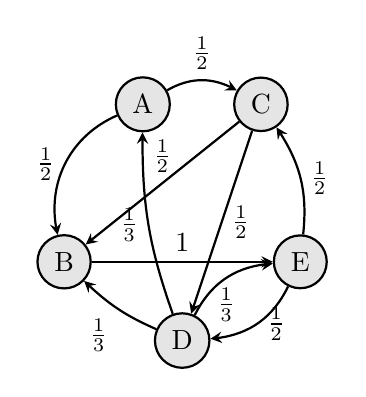
\begin{tikzpicture}[
        scale=0.5,
        ->,
        >=stealth,
        node distance=4cm,
        thick,
        main node/.style={circle, draw, fill=black!10, minimum size=4mm}
        ]

        % Nodes/States
        \node[main node] (A) at (0,4) {A};
        \node[main node] (B) at (-2,0) {B};
        \node[main node] (C) at (3,4) {C};
        \node[main node] (D) at (1,-2) {D};
        \node[main node] (E) at (4,0) {E};

        % Edges with reversed direction
        % From A to B (curving outwards)
        \path (A) edge [bend right=40] node[left] {$\frac{1}{2}$} (B);
        \path (A) edge [bend left=30] node[above] {$\frac{1}{2}$} (C);
        
        % From B to other states
        \path (C) edge node[above] {$\frac{1}{2}$} (B);
        \path (D) edge [bend left=10] node[below left] {$\frac{1}{3}$} (B);
        \path (D) edge [bend left=10] node[left] {$\frac{1}{3}$} (A);
        
        % From E to C (corrected direction)
        \path (E) edge [bend right=20] node[right] {$\frac{1}{2}$} (C);
        
        % From D to other states
        \path (C) edge  node[right] {$\frac{1}{2}$} (D);
        \path (D) edge [bend left=30] node[below] {$\frac{1}{3}$} (E);
        
        % From E to other states
        \path (B) edge node[above] {$1$} (E);
        \path (E) edge [bend left=30] node[right] {$\frac{1}{2}$} (D);
      \end{tikzpicture}
    \end{subfigure}
    \hfill 
    \begin{subfigure}[b]{0.48\textwidth}
      \centering
      \begin{equation}
        \begin{pmatrix}0&0&0&\frac{1}{3}&0\\
        \frac{1}{2}&0&\frac{1}{2}&\frac{1}{3}&0\\
        \frac{1}{2}&0&0&0&\frac{1}{2}\\
        0&0&\frac{1}{2}&0&\frac{1}{2}\\
        0&1&0&\frac{1}{3}&0\end{pmatrix}
      \end{equation}
    \end{subfigure}
    \caption{Markov chain graph and corresponding adjacency/transition matrix.}
    \label{fig:markov_chain}
  \end{figure}

  However, the theorem above requires the matrix to be strictly positive, which is often not true for Markov chains in general. This theorem does not hold true in the following example, 
  \begin{equation}
    A = \begin{pmatrix}
    0&0&0&\frac{1}{3} \\
    \frac{1}{2}&0&0&\frac{1}{3} \\
    0&0&0&\frac{1}{3} \\
    \frac{1}{2}&0&0&0
    \end{pmatrix} \implies A^{1000} 
        \begin{pmatrix}
    \frac{1}{4} \\ \frac{1}{4} \\ \frac{1}{4} \\ \frac{1}{4}
    \end{pmatrix} = 
        \begin{pmatrix}
    0 \\ 9/20 \\ 11/20 \\ 0
    \end{pmatrix}, \; A^{1001} 
        \begin{pmatrix}
    \frac{1}{4} \\ \frac{1}{4} \\\frac{1}{4} \\ \frac{1}{4}
    \end{pmatrix} = 
        \begin{pmatrix}
    0 \\ 11/20 \\ 9/20 \\ 0
    \end{pmatrix}
  \end{equation}
  That is, $A^N v$ oscillates between these two values. Furthermore, given three notes $A, B, C$ as such

  \begin{figure}[H]
    \centering 
    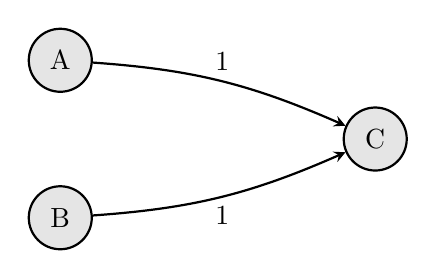
\begin{tikzpicture}[
      ->,
      >=stealth,
      node distance=3cm,
      thick,
      main node/.style={circle, draw, fill=black!10, minimum size=8mm}
      ]
      % Nodes
      \node[main node] (A) at (0,2) {A};
      \node[main node] (B) at (0,0) {B};
      \node[main node] (C) at (4,1) {C};

      % Edges with weight labels
      \path (A) edge [bend left=10] node[above] {$1$} (C);
      \path (B) edge [bend right=10] node[below] {$1$} (C);
    \end{tikzpicture}
    \label{fig:degenerate_markov_chain}
  \end{figure}
  the entries of the adjacency matrix is not well-defined. 
  \begin{equation}
     \begin{pmatrix} 0&0&? \\0&0&? \\1&1&?\end{pmatrix}
  \end{equation}
  Google CEO Larry Page actually developed a solution by implementing what he called a \textit{dampening factor}. Given stochastic matrix $B_{i j} = \frac{1}{N}$, he redefined the chain to be 
  \begin{equation}
    M = \alpha A + (1-\alpha) B, \; 0< \alpha < 1
  \end{equation}
  It is clear that $M$ is now a strictly positive stochastic matrix. The $\alpha$ is the dampening factor, and its optimal value is known to be about $0.67$. The value of the alpha determines how much of the data is "washed away." When $\alpha = 0$, none of the data is lost, and when $\alpha = 1$, all of the data is lost. 

  Due to the limitations of Perron's theorem, we can extend it with the following.

  \begin{theorem}[Frobenius Extension to Perron]
  Any $n \times n$ matrix $F \geq 0$, $F \neq 0$ has eigenvalue $\lambda$ such that
  \begin{enumerate}
      \item $\lambda \geq 0$ and $F h = \lambda h$, $h\geq 0$ \item every eigenvalue $\kappa$ satisfies: $|\kappa| \leq \lambda$ 
      \item if $|\kappa| = \lambda$, then 
      \begin{equation}
        \kappa = e^{\frac{2 \pi i k}{m}} \lambda, \; k, m \in \mathbb{Z}_+, \; m \leq n
      \end{equation}
  \end{enumerate}
  \end{theorem}

\subsection{Duality Theorem}

  In this section we will denote vector inequalities as entry-wise inequalities.Recall that elements of a vector space $X$ can be interpreted as column vectors, and elements of the dual of the vector space $X^\ast$ can be interpreted as row vectors. Therefore, value of $\phi$ at $x$ is denoted
  \begin{equation}
    \phi (x) = \phi_1 x_1 + \phi_2 x_2 + ... + \phi_n x_n
  \end{equation}
  Furthermore, the dual of $X^\ast$ is $X$ itself, and given that $Y$ is a linear subspace of $X$, the annihilator of $Y^\perp$ is $Y$. 
  \begin{equation}
    X = X^{**}, \;\; Y = Y^{\perp\perp}
  \end{equation}
  Suppose $Y$ is defined as the linear space spanned by the $m$ vectors $y_1, y_2, ..., y_m$ in $X$. That is, $Y$ consists of all vectors $y$ of the form
  \begin{equation}
    y = \sum_{j=1}^m a_j y_j
  \end{equation}
  It is clear by linearity that $\phi$ belongs to $Y^\perp$ if and only if
  \begin{equation}
    \phi (y_j) = 0, \;\; j = 1, 2, ..., m
  \end{equation}
  That is, a vector $y$ can be written as a linear combination of $m$ given vectors $y_j$ if and only if every $\phi$ that annihilates the $m$ vectors a also annihilates $0$. Now, we state a theorem that allows us to check if a vector $y$ can be written as a \textit{nonnegative} linear combinations of the $y_j$s. 

  \begin{theorem}
  A vector $y$ can be written as a linear combination of given vectors $y_j$ with nonnegative coefficients if and only if every $\zeta \in X^\ast$ that satisfies 
  \begin{equation}
     \zeta (y_j) \geq 0, \;\; j = 1, 2, ..., m
  \end{equation}
  also satisfies 
  \begin{equation}
    \zeta (y) \geq 0
  \end{equation}
  \end{theorem}
  \begin{proof}
  The proof is not the easiest to construct rigorously, but it can be visualized easily. 
  \end{proof}

  \begin{corollary}
  Given a $n \times m$ matrix $Y$, a vector $y$ with $n$ components can be written in the form 
  \begin{equation}
    y = Y p, \;\; p \geq 0
  \end{equation}
  if and only if every row vector $\zeta$ that satisfies 
  \begin{equation}
    \zeta Y \geq 0
  \end{equation}
  also satisfies 
  \begin{equation}
    \zeta y \geq 0
  \end{equation}
  \end{corollary}

  \begin{theorem}
  Given an $n \times m$ matrix $Y$ and a column vector $y$ with $n$ components, the inequality 
  \begin{equation}
    y \geq Y p, \;\; p \geq 0
  \end{equation}
  is satisfied if and only if every $\zeta$ that satisfies
  \begin{equation}
    \zeta Y \geq 0, \;\; \zeta \geq 0
  \end{equation}
  also satisfies 
  \begin{equation}
    \zeta y \geq 0
  \end{equation}
  \end{theorem}

  \begin{theorem}[Duality Theorem]
  Let $Y$ be a given $n \times m$ matrix, $y$ a given column vector with $n$ components, and $\gamma$ a given row vector with $m$ components. Let 
  \begin{equation}
    S = \sup_p \{\gamma p\}
  \end{equation}
  for all column vectors $p$ with $m$ components satisfying $y \geq Y p, \; p \geq 0$. A well-defined such $p$ is called \textbf{supremum admissible}. Additionally, let 
  \begin{equation}
    s = \inf_\zeta \{ \zeta y\}
  \end{equation}
  for all row vectors $\zeta$ with $n$ components satisfying $\gamma \leq \zeta Y, \; \zeta \geq 0$. A well-defined such $\zeta$ is called \textbf{infimum admissible}. Given that admissible vectors $p$ and $\zeta$ exist, then $S$ and $s$ are finite and 
  \begin{equation}
    S = s
  \end{equation}
  \end{theorem}

\subsection{Alternating Sign Matrices}

  We now describe a generalization of permutation matrices. While these kinds of matrices haven't been studied deeply, its applications lie in measuring the computational complexity of the Dodgson Condensation method for computing matrix determinants. The set of alternating sign matrices also forms a bijection with combinatorial objects, such as plane partitions, aztec diamonds, ice models, etc. 

  \begin{definition}
  A matrix with elements $0, -1, 1$ where nonzero entries must alternate in the following pattern: $1, -1, 1, ..., -1, 1$ (i.e. begin and end with $1$) is called an \textbf{alternating sign matrix}. This means that every row and column must add up to $1$. 
  \end{definition}

  \begin{example}
  The following are alternating sign matrices. 
  \[\begin{pmatrix}
  0&1&0&0\\1&-1&0&1\\0&1&0&0\\0&0&1&0
  \end{pmatrix}, \begin{pmatrix}
  0&1&0\\1&-1&1\\0&1&0
  \end{pmatrix}\]
  \end{example}

  As with permutation matrices, we would like to calculate how many $n \times n$ alternating sign matrices there are for a given $n$. Let the set of all $n \times n$ alternating sign matices be denoted
  \begin{equation}
    \text{ASM}(n)
  \end{equation}

  \begin{proposition}[Alternating Sign Matrix Conjecture (Proved)]
  The number of $n \times n$ alternating sign matrices is the following. 
  \begin{equation}
    \text{card ASM}(n) = \prod_{k=0}^{n-1} \frac{(3k+1)!}{(n+k)!}
  \end{equation}
  \end{proposition}

  We now define a bijection between ASMs and another type of $n \times n$ matrix. Given $A \in \text{ASM}(n)$, we define $f: \text{ASM}(n) \longrightarrow \text{Mat}(n, \{0,1\})$ such that
  \begin{equation}
    \big(f(A)\big)_{ij} = \sum_{k=i}^n (a)_{kj}
  \end{equation}
  Basically, we leave the bottom row untouched and for each element on upper rows, we sum that element with all of the elements strictly below it. For example, 
  \[\begin{pmatrix}
  0&1&0&0\\1&-1&0&1\\0&1&0&0\\0&0&1&0
  \end{pmatrix} \mapsto \begin{pmatrix}
  1&1&1&1\\1&0&1&1\\0&1&1&0\\0&0&1&0
  \end{pmatrix}\]

  \begin{theorem}
  The set of matrices $\im(f) \subset \text{Mat}(n, \{0, 1\})$ is bijective to the set of $n \times n$ 6-vertex (or Ice-type) models, which are used to model crystal lattices for hydrogen bonds. 
  \end{theorem}


\section{Numerical Methods in Solving Linear Systems}

  In this section, we will concern ourselves with a system of equations with only \textit{one solution}, represented by the matrix equation
  \[A x = b\]
  where $A$ is an invertible square matrix, $b$ some given vector, and $x$ the vector of unknowns to be determined. 

  An algorithm for solving the system takes as inputs the matrix $A$ and vector $b$ and outputs some approximation to the solution $x$. However, with billions of arithmetic operations on top of each other, the errors can accumulate. Algorithms for which this does not happen are said to be \textbf{arithmetically stable}. 

  The use of finite digit arithmetic places an absolute limitation on the accuracy with which the solution can be determined. To demonstrate this, let us imagine a change $\delta b$ being made in the vector $b$, which causes a corresponding change in $x$, denoted $\delta x$. 
  \[A(x + \delta x) = b + \delta b \implies A \delta x = \delta b\]
  To compare the changes in $x$ with the changes in $b$, we define the following variable. 
  \begin{definition}
  The \textbf{relative change in x with the relative change in $b$} is the quantity
  \[\frac{|\delta x|}{|x|} \bigg/ \frac{|\delta b|}{|b|}\]
  where the norm is convenient for the problem (usually a numerical approximation of the Euclidean norm for floating point numbers). We will assume the use of the Euclidean norm from now on. We can rewrite the value as the expression below with the following upper bound, denoted by $\kappa (A)$, called the \textbf{condition number}. 
  \[\frac{|b|}{|x|} \frac{|\delta x|}{|\delta b|} = \frac{|Ax|}{|x|} \frac{|A^{-1} \delta b|}{|\delta b|} \leq |A||A^{-1}| \equiv \kappa (A)\]
  where $|A|$ is the matrix norm of $A$. 
  A high value of this relative change would mean that small perturbations in $b$ would cause large changes in $x$.
  \end{definition}

  Note that $\kappa(A) \geq 1$. Notice also that the higher the condition number $\kappa (A)$, the harder it is to solve the equation $A x = b$, and $\kappa(A) = \infty$ when $A$ is not invertible. For a $k$-digit floating point arithmetic, the relative error in $b$ can be as large as $10^{-k}$, meaning that the relative error in $x$ can be as large as $10^{-k} \kappa (A)$. 

  Let $\beta$ be the largest absolute value of the eigenvalues of $A$ and $\alpha$ as the smallest absolute value of the eigenvalues of $A$. Then 
  \[\beta \leq |A|, \frac{1}{\alpha} \leq |A^{-1}| \implies \frac{|\beta|}{|\alpha|} \leq \kappa(A)\]


  \begin{definition}
  An algorithm that generates an exact solution after a finite number of arithmetic steps is called a \textit{direct method} (e.g. Gauss Elimination). An algorithm that generates successive approximations that converge onto the solution is called an \textit{iterative method}. 
  \end{definition}

  The methods mentioned in this section will be iterative. 
  \begin{definition}
  Let $\{ x_n\}$ be the sequence of approxmations generated by such an algorithm. The deviation of $x_n$ from the true value $x$ is caelled the \textbf{error at the $n$th stage}, denoted by $e_n$. 
  \[e_n \equiv x_n - x\]
  The amount by which the $n$th approximation fails to satisfy the equation $Ax = b$ is called the $n$th residual, denoted by $r_n$. 
  \[r_n \equiv A x_n - b\]
  Error and residual are related by the equation. 
  \[r_n = A e_n\]
  \end{definition}
  Note that since we do not know $x$, the error cannot be calculated, but the residuals can be. We further restrict our scope to solving linear systems in which $A$ is real, positive, and self-adjoint. Clearly, we already know that $|A| = \beta$, and since $A$ is positive, we can conclude that 
  \[|A^{-1}| = \frac{1}{\alpha}\]
  which implies that
  \[\kappa(A) = \frac{\beta}{\alpha}\]

\subsection{Method of Steepest Descent}

  Assume that $n \times n$ matrix $A$ is self-adjoint.
  \begin{theorem}
  The solution of $Ax = b$ minimizes the functional 
  \[E (y) \equiv \frac{1}{2} (y, A y) - (y, b)\]
  where $(\cdot, \cdot)$ is the Euclidean dot product. That is, the solution $x$ is
  \[x = \min \big\{ E(y) \big\} = \min \Big\{ \frac{1}{2} (y, Ay) - (y, b) \Big\}\]
  \end{theorem}
  \begin{proof}
  Add to $E(y)$ a constant, that is a term independent of $y$ to define a new function $F$. 
  \[F(y) \equiv E(y) + \frac{1}{2} (x, b)\]
  Then, by self adjointness of $A$, we can express $F(y)$ as 
  \begin{align*}
      F(y) & = \frac{1}{2} (y, Ay) - (y, b) + \frac{1}{2} (x, b) \\
      & = \frac{1}{2} (y, Ay) - \frac{1}{2} (y, Ax) + \frac{1}{2} (Ax, x) - \frac{1}{2} (Ay, x) \\
      & = \frac{1}{2} \big( y, A(y-x)\big) + \frac{1}{2} \big( A(x-y), x\big) \\
      & = \frac{1}{2} \big( y - x, A(y - x)\big) 
  \end{align*}
  Since $F(x) = 0$ and $F(x) \geq 0$ (since it is an inner product with repsect to $y-x$), $F(y)$, and also $E(y)$, takes a minimum at $y =x$. 
  \end{proof}

  Now to actually compute the value of $x$, we us the method of steepest descent. Note that $E: \mathbb{R}^m \longrightarrow \mathbb{R}$, so we can utilize ordinary calculus on it. The gradient of $E$ can be computed by the formula 
  \[\text{grad}\,E(y) = A y - b\]
  So, if our $n$th approximation is $x_n$, then the $(n+1)$st approximation, $x_{n+1}$, is calculated as
  \[x_{n+1} = x_n - s (Ax_n - b)\]
  where $s$ is the step length in the direction $-$grad$\,E$. By calculating the residual $r_n = A x_n - b$, we can rewrite the above to
  \[x_{n+1} = x_n - s r_n\]
  Rather than keeping $s$ constant, we can actually determine an optimal value of $s$ at the $n$th step, denoted $s_n$, which minimizes $E(x_{n+1})$. This quadratic minimum problem is easily solved, since
  \begin{align*}
      E(x_{n+1}) & = \frac{1}{2} \big(x_n - s r_n, A(x_n - s r_n) \big) - \big( x_n - s r_n, b\big) \\
      & = E(x_n) - s (r_n, r_n) + \frac{1}{2} s^2 (r_n A r_n)
  \end{align*}
  By taking the derivative and computing the value of $s$ where $E (x_{n+1}) = 0$, we see that the minimum is reached when 
  \[s = s_n \equiv \frac{(r_n, r_n)}{(r_n, A r_n)}\]

  \begin{theorem}
  The sequence of approximations $\{x_n\}$, with $s$ optimized to be $s_n$, converges to the solution of $A x = b$. 
  \end{theorem}

  The error bound for this algorithm is 
  \[||e_n||^2 \leq \frac{2}{\alpha} \bigg( 1-\frac{1}{\kappa(A)} \bigg)^n F(x_0)\]
  which shows that the error $e_n$ tends to $0$ in $\mathbb{R}^m$. However, this algorithm has a very slow rate of convergence for large $\kappa(A)$. 

\subsection{Method of Chebyshev Polynomials}

  the disadvantage of the method of steepest descent mentioned in the end of the last subsection renders it quite outdated and obsolete. this next method has a much better error bound that can handle large values of $\kappa$ more efficiently. however, we will need a positive lower bound $m$ for the smallest eigenvalue of $a$ and an upper bound $m$ for the largest eigenvalue. that is, 
  \[m \leq \alpha, \beta \leq m\]
  and all the eigenvalues of $a$ lie in the interval $[m, m]$. it follows that
  \[\kappa = \frac{\beta}{\alpha} < \frac{m}{m}\]
  we generate the same sequence of approximations $\{x_n\}$ by the same recursion formula
  \[x_{n+1} = x_n - s(a x_n - b) \iff x_{n+1} = (i - s_n a) x_n + s_n b\]
  since the solution of $x$ satisfies the formula; that is, since $x = (i - s_n a) x + s_n b$, we subtract this equation from the top to get
  \[e_{n+1} = (i - s_n a) e_n\]
  doing this recursively, we can deduce an explicit formula 
  \[e_n = p_n (a) e_0 = \prod_{n=1}^n (1 - s_n a)\]
  this allows us to estimate the size of $e_n$. 
  \[||e_n|| \leq ||p_n (a)|| ||e_0||\]
  the norm of a self adjoint matrix $a$ is the largest $|a|$, where $a$ is the eigenvalue, and the spectral mapping theorem states that the eigenvalues $p$ of $p_n (a)$ are of the form $p = p_n (a)$, where $a$ is an eigenvalue of $a$. this means that
  \[||a|| \leq \max_{m \leq a \leq m} |a| \implies ||p_n (a)|| \leq \max_{m \leq a \leq m} |p_n (a)|\]
  so, we are left with the bound
  \[||e_n|| \leq ||e_0|| \max_{m \leq a \leq m} |p_n (a)|\]
  to get the best estimate of $e_n$, we have to choose the $s_1, s_2, ..., s_n$ so that the polynomial $p_n$ has a small maximum on the interval $[m, m]$. note that the polynomial $p_n$ satisfies the normalizing condition 
  \[p_n(0) = 1\]
  to find such a polynomial, we must first define chebyshev polynomials. 

  \begin{definition}
  the \textbf{$n$th chebyshev polynomial} $t_n$ is defined for $-1 \leq u \leq 1$ by
  \[t_n (u) = \cos (n \theta), \;\; u = \cos(\theta)\]
  \end{definition}

  \begin{proposition}
  among all polynomials $p_n$ of degree $n$ that satisfy $p_n (0) = 1$, the one that has the smallest maximum on $[m, m]$ is the \textit{rescaled chebyshev polynomial} that rescales values from $[-1, 1]$ to the interval $[m, m]$ while preserving the condition that $p_n (0) = 1$. this polynomial is expressed as
  \[p_n (a) \equiv t_n \bigg( \frac{m+m-2a}{m-m} \bigg) \bigg/ t_n \bigg(\frac{m+m}{m-m} \bigg)\]
  \end{proposition} 
  now, assuming that $m/m \approx \kappa$, 
  \[t_n \bigg( \frac{m+m}{m-m} \bigg) = t_n \bigg(\frac{\frac{m}{m} + 1}{\frac{m}{m}-1} \bigg) \approx t_n \bigg(\frac{\kappa + 1}{\kappa - 1} \bigg)\]
  since $|t_n (u)| \leq 1$ for $|u| \leq 1$, this also implies that
  \[t_n \bigg( \frac{m + m - 2a}{m-m} \bigg) \leq 1\]
  combining this together, we get
  \[||e_n|| \leq ||e_0|| \max_{m \leq a \leq m} |p_n (a)| = ||e_0|| \bigg/ t_n \bigg( \frac{\kappa+1}{\kappa-1} \bigg)\]
  it is a fact that higher order chebyshev polynomials tend to infinity faster once the value reaches out of $[-1, 1]$, meaning that as $n \rightarrow \infty$, $t_n\big( (\kappa+1)/(\kappa-1)\big)$ will also tend to infinity (note that $(\kappa+1)/(\kappa-1)$ is a constant, implying that $e_n$ tends to $0$ as $n$ tends to infinity. the error bound for $e_n$ is given by the following 
  \[||e_n|| \leq 2 \bigg( 1 + \frac{2}{\sqrt{\kappa}} \bigg)^{-n} ||e_0|| \approx 2 \bigg( 1 - \frac{2}{\sqrt{\kappa}} \bigg)^{n} ||e_0||\]
  once again, this confirms that $e_n \rightarrow 0$ as $n \rightarrow \infty$. furthermore, when $\kappa$ is large, the error bound works with $\sqrt{\kappa}$, which is must smaller than $\kappa$ itself. so, $e_n$ converges much faster through this algorithm than through the method of steepest descent. 


\section{Tensors as Multilinear Maps}

  There are multiple ways to construct tensor product spaces. Note that all the constructions are equivalent and will lead to the exact same properties of tensors. The first method defines tensors outright as multilinear maps, without the need for a basis. 

\subsection{Tensor Product of Two Spaces}

  \begin{definition}
  The tensor product of two vector spaces $V$ and $W$ is a vector space, denoted $V \otimes W$, created by the bilinear map 
  \[\otimes: V \times W \longrightarrow V \otimes W, \; (x, y) \mapsto x \otimes y\]
  That is, 
  \[V \otimes W \equiv \{ x \otimes y \; | \; x \in V, y \in W\} \]
  where the elements of $V \otimes W$ are called \textbf{tensors}. Note that since we have defined the operation $\otimes$ to be bilinear, it satisfies the properties
  \begin{enumerate}
      \item $(u_1 + u_2) \otimes v = u_1 \otimes v + u_2 \otimes v$
      \item $v \otimes (u_1 + u_2) = v \otimes u_1 + v \otimes u_2$
      \item $(\lambda u) \otimes v = u \otimes (\lambda v) = \lambda (u \otimes v)$ 
  \end{enumerate}
  Moreover, each tensor $x \otimes y$ is itself a bilinear operator
  \[x \otimes y: V^* \otimes W^* \longrightarrow \mathbb{F}\]
  \end{definition}

  Using these properties we will deduce further qualities of tensor product spaces. First, given a basis $\{e_i\}$ of $n$-dimensional space $V$ and $\{f_j\}$ of $m$-dimensional space $W$, we can construct a basis 
  \[\{e_i \otimes f_j \; | \; 1 \leq i \leq n, 1 \leq j \leq m\}\]
  of $V \otimes W$ using only the bilinearity properties of $\otimes$. 

  \begin{example}
  Let $V^*$ be a 4-dimensional vector space with basis $\{ e^0, e^1, e^2, e^3\}$. Then the basis of $V^* \otimes V^*$ is
  \begin{align*} 
  \{e^0 \otimes e^0, \; e^0 \otimes e^1, \;e^0 \otimes e^1, \;e^0 \otimes e^1, \\
  e^1 \otimes e^0,\; e^1 \otimes e^1,\; e^1 \otimes e^2,\; e^1 \otimes e^3, \\
  e^2 \otimes e^0,\; e^2 \otimes e^1,\; e^2 \otimes e^2,\; e^2 \otimes e^3, \\
  e^3 \otimes e^0,\; e^3 \otimes e^1,\; e^3 \otimes e^2,\; e^3 \otimes e^3\}
  \end{align*}
  \end{example}

  That is, every tensor can be expressed as a linear combination of these vectors, which implies
  \[\dim{V \otimes W} = (\dim{V}) (\dim{W})\]
  By equality of dimensionality and bilinearity, it is obvious that
  \[V \otimes W \simeq \text{Hom}(V \times W, \mathbb{F})\]
  In fact, they are naturally isomorphic. 

  Notice that we still haven't actually defined how to "calculate" using the operator $x \otimes y$. It turns out that defining a tensor product is unique up to isomorphism. That is, if $(V \otimes W, \otimes_1)$ and $(V \otimes W, \otimes_2)$ are two tensor product spaces sufficing bilinearity, then $V \otimes_1 W \simeq V \otimes_2 W$. This result is formally stated in the proposition below. 

  \begin{proposition}[Universal Property of 2-tensors]
  With this constructed basis, we can claim that for every map $\varphi: V \times W \longrightarrow \mathbb{F}$, there exists a unique linear map $\psi: V \otimes W \longrightarrow \mathbb{F}$ such that 
  \[\varphi (x, y) = \psi (x \otimes y) \; \forall x \in V, y \in W\]
  \end{proposition}
  \begin{proof}
  Since $\{e_i \otimes f_j\}$ is a basis for $V \otimes W$, we know that every element $z \in V \otimes W$ decomposes uniquely into 
  \[z = \sum_{i, j} z_{i j} e_i \otimes f_j, \; z_{i j} \in \mathbb{F}\]
  Thus, by linearity it suffices to define these maps for the basis vectors. This linear map is determined as 
  \[\psi (e_i \otimes f_j) = \varphi (e_i, f_j)\]
  \end{proof}
  Denoting the map that is defined by taking all $e_i \otimes f_j \mapsto (e_i, f_j)$ as $S$, we can see that $S$ is clearly an isomorphism defined such that the diagram below commutes. 
  \[\begin{tikzcd}
      V \otimes W \arrow{r}{\psi} \arrow{d}{S} & \mathbb{F} \\
      V \times W \arrow{ru}{\varphi}
  \end{tikzcd}\]
  That is, the unique isomorphism $S$ exists that determines $\psi$ such that 
  \[\psi = \varphi \circ S \] 
  which means that all definitions of $\otimes$ are equivalent under $S$. Note further that $S$ determines the isomorphism 
  \[(V \otimes W)^* \equiv \text{Hom}(V \otimes W, \mathbb{F}) \simeq \text{Hom}(V \times W, \mathbb{F})\]
  Therefore, it does not matter how we choose to concretely define the operator $x \otimes y$ for computations. However, it is customary to define it as
  \[(x \otimes y) (\alpha, \beta) = \alpha (x) \cdot \beta (y), \; \alpha \in V^*, \beta \in W^*\]
  Given $x \otimes y \in V \otimes W$, we can also choose to input elements "partially." That is, if we only input one vector $\alpha \in V^*$ into $x \otimes y$, we get
  \[(x \otimes y) (\alpha, \cdot) = \alpha(x) y (\cdot) = \alpha (x) y \in W\]
  meaning that the isomorphisms below are all canonical
  \[V \otimes W \simeq \text{Hom}(V \times W, \mathbb{F}) \simeq \text{Hom}(V^*, W)\]
  This means that
  \[V^* \otimes W \simeq \text{Hom}(V, W)\]
  That is, an element $\alpha \otimes y \in V^* \otimes W$ is a linear map from $V$ to $W$! We will focus a bit more on elements of $V^* \otimes W$. Given the previous bases $e_i$ and $f_j$ for $V$ and $W$, let $\{\epsilon_i\}$ be the dual basis for $V^*$. Then, the tensor $\alpha \otimes w \in V^* \otimes W$ can be represented as 
  \begin{align*}
      \alpha \otimes w & \equiv \bigg(\sum_i \alpha_i \epsilon_i \bigg) \otimes \bigg( \sum_j w_j f_j \bigg) \\
      & = \sum_{i, j} \alpha_i w_j \, \epsilon_i \otimes f_j = \sum_{i, j} A_{i j} \, \epsilon_i \otimes f_j
  \end{align*}
  In fact, the $A_{i j}$ are precisely the $i j$th components of the matrix representation of linear operator $\alpha \otimes y$ with respect to basis $\{\epsilon_i\}$ and $\{f_j\}$. Indeed,
  \begin{align*}
      (\alpha \otimes y)(e_j) & = \bigg( \sum_{i, j} e_i \otimes f_j \bigg) e_j \\
      & = \sum_{i, j} A_{i j} e_i \cdot \delta^j_j = \sum_{i} A_{i j} e_i
  \end{align*}
  which is consistent with the column space interpretation of matrix multiplication discussed in the beginning of Chapter 4. The realization of this tensor product between a covector and a vector is realized as an \textbf{outer product}. 

  \begin{definition}
  Given vector spaces $U, V$ with defined bases in each of them, the \textbf{outer product} of two vectors $u \in U$ and $v \in V$ is defined
  \[u \otimes v \equiv u v^T \equiv \begin{pmatrix}
  u_1 \\ u_2 \\ ... \\ u_m
  \end{pmatrix} \otimes \begin{pmatrix}
  v_1 & ... & v_n
  \end{pmatrix} = \begin{pmatrix}
  u_1 v_1 & ... & u_1 v_n \\
  u_2 v_1 & ... & u_2 v_n \\
  ... & ... & ... \\
  u_m v_1 & ... & u_m v_n 
  \end{pmatrix}\]
  Note that the $\otimes$ symbol in here represents the outer product, not the tensor product. Note that the tensor rank of the outer product of two vectors is $(2,0)$. 
  \end{definition}

  Abstractly speaking, the outer product of $u \in U$ and $v \in V$ is the element $u \otimes v \in U \otimes V$, which is a rank-(2,0) tensor, not a rank-(1,1) tensor! Just because it "looks" like a matrix, $u \otimes v$ should not be interpreted as a linear map. Such a $m \times n$ matrix could really be the realization of either a (2,0) tensor, (1,1) tensor, or a (0,2) tensor. 

  However, if $U$ is an inner product space, then it is possible to define $u \times v$ as a linear map from $U \longrightarrow W$. The structure of the inner product on $U$ allows us to define the canonical isomorphism $\phi$ between $U$ and $U^*$. Then, we can define the canonical injections $i: U \longrightarrow U \otimes V$ and $j: U^* \longrightarrow U^* \otimes V$ to get the commutative diagram 

  \[\begin{tikzcd}
      U \otimes V \arrow{r}{\gamma} & U^* \otimes V \\
      U \arrow{u}{i} \arrow{r}{\phi} & U^* \arrow{u}{j}
  \end{tikzcd}\]
  Given that 
  \[\phi(u) \equiv l \text{ such that } (u, x) = l(x) \forall x \in U\]
  we can define the mapping $\gamma: j \phi i^{-1}$ such that 
  \[\gamma (u \otimes v) \equiv \phi(u) \otimes v \equiv l \otimes v \in U^* \otimes V\]
  which is ultimately a linear mapping from $U \longrightarrow V$ since
  \[l \otimes v (u_0, \cdot) \equiv l(u_0) v(\cdot)\]
  with $l(u_0) \in \mathbb{F}$ and $v(\cdot)$ a vector. This proves the following theorem. 

  \begin{proposition}
  The matrix rank of the outer product of any 2 vectors is $1$. 
  \end{proposition}
  \begin{proof}
  Trivial.
  \end{proof}

  We can extrapolate and see that for higher order tensor products, we would get an $n$-dimensional array of scalars. A matrix is a $2$-dimensional array of numbers since it is the tensor product of two vectors. 

  \begin{definition}
  Given vector spaces $U, V$ with defined bases in each of them, the \textbf{Kronecker product} of two vectors $u \in U$ and $v \in V$ is defined
  \[u \otimes_{Kron} v \equiv \begin{pmatrix}
  u_1 \\ u_2 \\ ... \\ u_m
  \end{pmatrix} \otimes \begin{pmatrix}
  v_1 & ... & v_n
  \end{pmatrix} = \begin{pmatrix}
  u_1 v_1 \\ u_1 v_2 \\ ... \\ u_m v_{n-1} \\ u_m v_n 
  \end{pmatrix}\]
  \end{definition}

  Clearly, the outer product and Kronecker product are closely related, and we can interpret the Kronecker product as a form of "vectorization" or "flattening out" of the outer product. 

\subsection{Higher Order Tensor Product Spaces}

  Since $U \otimes W$ is a vector space itself, we can multiply it further to create higher order tensor product spaces. 
  \[U \otimes W \otimes U \otimes ...\]
  Note that by construction, the operation of tensor product on vector spaces is commutative and associative in the sense that 
  \[V \otimes W \simeq W \otimes V\]
  and 
  \[(U \otimes V) \otimes W \simeq U \otimes (V \otimes W) \simeq U \otimes V \otimes W \]
  which allows us to write tensor products of any finite number of vector spaces $V_1, V_2, ..., V_n$ without parantheses. By induction, we can keep constructing higher order tensor products as such 
  \[V_1 \otimes V_2 \rightarrow (V_1 \otimes V_2) \otimes V_3 \rightarrow \big((V_1 \otimes V_2) \otimes V_3 \big) \otimes V_4 \rightarrow ...\]
  to get the tensor product space
  \[\bigotimes_{i=1}^{n} V_{i} \equiv V_1 \otimes V_2 \otimes ... \otimes V_n\]
  with tensors in the form 
  \[ \bigotimes_{i=1}^{n} v_{i} \equiv v_{1} \otimes v_{2} \otimes v_{3} \otimes ... \otimes v_{n}; \; v_{i} \in V_{i}\]
  defined as the following multilinear map 
  \[ \bigotimes_{i=1}^{n} v_{i}: \prod_{i=1}^{n} V_{i}^{*} \longrightarrow \mathbb{F}, \;\;\; \bigg( \bigotimes_{i=1}^{n} v_{i} \bigg) \big( l_{1}, l_{2}, ..., l_{n} \big) \equiv \prod_{i=1}^{n} v_{i}(l_{i}), \; l_i \in V_i^* \]
  This map can then be used to easily see the following statement
  \[\bigotimes_{i=1}^n V_i \simeq \text{Hom}\Big( \prod_{i=1}^n V_i^*, \mathbb{F} \Big)\]
  Similarly to the section about the tensor product of two spaces, we can "partially" fill in the inputs of a general tensor $v_1 \otimes v_2 \otimes ... \otimes v_n$ to interpret them as multilinear operators that can take in $k$ vectors and output $n-k$ vectors. That is, tensors (written as $\tau$ below) are multilinar maps from a cartesian product of vector spaces to a tensor product of vector spaces. 
  \[\tau: V_1 \times ... \times V_n \longrightarrow W_1 \otimes ... \otimes W_m \]
  For example, 
  \[\text{Hom}\Big( \prod_{i=1}^n V_i^*, \mathbb{F} \Big) \simeq 
  \text{Hom}\Big( \prod_{i=2}^n V_i^*, V_1 \Big) \simeq 
  \text{Hom}\Big( \prod_{i=3}^n V_i^*, V_1 \otimes V_2 \Big) \simeq ... \]
  Furthermore, we can generalize the universal property of two tensors to the following proposition, which is also called the \textbf{fundamental principle of tensor algebra}. 

  \begin{proposition}[Universal Property]
  Given a linear mapping $\varphi: V_1 \times ... \times V_n \longrightarrow \mathbb{F}$, there exists a unique linear map $\psi: V_1 \otimes ... \otimes V_n \longrightarrow \mathbb{F}$. That is, 
  \[\text{Hom}\Big( \bigotimes_{i=1}^n V_i, \mathbb{F} \Big) \equiv \bigg( \bigotimes_{i=1}^n V_i \bigg)^* \simeq \text{Hom}\Big(\prod_{i=1}^n V_i, \mathbb{F}\Big)\]
  \end{proposition}

  \begin{definition}
  Given that 
  \[ \{ e_{i_{j}}\}_{i_{j}=1}^{k_{j}} \text{ of } V_{j},\; j = 1, 2, ..., n\]
  are $n$ sets of bases for each $V_{j}$, 
  \[ \{ \bigotimes_{j=1}^{n} e_{i_{j}} \}_{i_{1}, ..., i_{n}} \text{ is a basis of } \bigotimes_{j=1}^{n} V_{j}\]
  \end{definition}

  \begin{proposition}
  Given vector spaces $V_1, V_2, ..., V_n$, 
  \[ \dim \bigotimes_{i=1}^{n} V_i = \prod_{i=1}^{n} \dim V_{i}\]
  \end{proposition}
  \begin{proof}
  This follows naturally from the construction of the basis.
  \end{proof}

  We move on to talk about something quite enlightening: the tensor product of linear operators, which are themselves tensors. 

  \begin{definition}
  Given linear operators $A \in $ End$(V)$, $B \in $ End$(W)$, we can construct the linear operator 
  \[A \otimes B \in \text{End}(V \otimes W)\] 
  such that 
  \[(A \otimes B) (x \otimes y) \equiv A x \otimes B y \in V \otimes W\]
  Notice that since $A, B$ are linear operators, they are tensors. More specifically, $A \equiv \alpha \otimes u$ and $B \equiv \beta \otimes v$, so
  \begin{align*}
      (A \otimes B) (x \otimes y) & \equiv A x \otimes B y \\
      & = (\alpha \otimes u) x \otimes (\beta \otimes v) y \\
      & = \alpha (x) \beta (y) \, u \otimes v \\
      & = \big((\alpha \otimes \beta)(x \otimes y)\big) (u \otimes v)(\cdot, \cdot) \\
      & = \big((\alpha \otimes \beta) \otimes (u \otimes v)\big) \big((x \otimes y), (\cdot \otimes \cdot)\big) \\
      & = \big((\alpha \otimes \beta) \otimes (u \otimes v)\big)(x \otimes y) 
  \end{align*}
  $\implies A \otimes B \equiv \alpha \otimes \beta \otimes u \otimes v$. 
  \end{definition}
  We will work through an example that gives the matrix representation of the tensor product of linear mappings. For simplicity, let us work with the example when 
  \[A = \begin{pmatrix}
  a_{11} & a_{12} \\ a_{21} & a_{22}
  \end{pmatrix}, \; B = \begin{pmatrix}
  b_{11} & b_{12} \\ b_{21} & b_{22}
  \end{pmatrix}\]
  Given that $U$ has basis $\{u_1, u_2\}$ and $V$ has basis $\{v_1, v_2\}$, $U \otimes V$ will have basis 
  \[\{u_1 \otimes v_1, u_1 \otimes v_2, u_2 \otimes v_1, u_2 \otimes v_2\}\]
  We then define the induced linear mapping $A\otimes B: U \otimes V \longrightarrow U \otimes V$ by defining it on its basis vectors. Note that the linear mapping $(A \otimes B)(u\otimes v)$ must be an element of $U \otimes V$, implying that it is defined
  \[(A \otimes B)(u\otimes v) \equiv Au \otimes Bv\]
  This is called the \textbf{tensor product} of operators $A$ and $B$.
  So, the tensor product of matrices $A$ and $B$ can be calculated
  \begin{align*}
      (A \otimes B) (u_1 \otimes v_1) &= (a_{11} u_1 + a_{21} u_2) \otimes (b_{11} v_1 + b_{21} v_2) \\
      & = a_{11} b_{11} (u_1 \otimes v_1) + a_{11} b_{21} (u_1 \otimes v_2) \\
      & + a_{21} b_{11} (u_2 \otimes v_1) + a_{21} b_{21} (u_2 \otimes v_2) \\
      ... & = ... \\
      (A \otimes B) (u_2 \otimes v_2) & = (a_{12} u_1 + a_{22} u_2) \otimes (b_{12} v_1 + b_{22} v_2) \\
      & = a_{12} b_{12} (u_1 \otimes v_1) + a_{12} b_{22} (u_1 \otimes v_2) \\
      & + a_{22} b_{12} (u_2 \otimes v_1) + a_{22} b_{22} (u_2 \otimes v_2) 
  \end{align*}
  In matrix form, this results in the $4\times 4$ matrix (also in block form)
  \[A \otimes B \equiv \begin{pmatrix}
  a_{11} b_{11} & a_{11} b_{12} & a_{12} b_{11} & a_{12} b_{12} \\
  a_{11} b_{21} & a_{11} b_{22} & a_{12} b_{21} & a_{12} b_{22} \\
  a_{21} b_{11} & a_{21} b_{12} & a_{22} b_{11} & a_{22} b_{12} \\
  a_{21} b_{21} & a_{21} b_{22} & a_{22} b_{21} & a_{22} b_{22} 
  \end{pmatrix} = \begin{pmatrix}
  a_{11} B & a_{12} B \\
  a_{21} B & a_{22} B 
  \end{pmatrix}\]
  representing the linear transformation from $U \otimes V$ to itself under the basis $\{u_i \otimes v_j\}$. 
  \begin{proposition}
  In general,the tensor product of matrices $A \in $ End$(V)$ and $B \in $ End$(W)$ (with basis of $V, W$ defined) is the $(m n) \times (m n)$ matrix
  \[A \otimes B \equiv \begin{pmatrix}
  a_{11} B & a_{12} B & ... & a_{1n} B \\
  a_{21} B & a_{22} B & ... & a_{2n} B \\
  ... & ... & ... & ... \\
  a_{n1} B & a_{n2} B & ... & a_{nn} B 
  \end{pmatrix}\]
  represented in block form. 
  \end{proposition}

  \begin{proposition}
  \begin{align*}
      & \Tr{A \otimes B} = \Tr{A} \cdot \Tr{B} \\
      & \det{A \otimes B} = (\det{A})^n (\det{B})^m
  \end{align*}
  \end{proposition}

  \begin{proposition}
  For finite dimensional space $V$ and $W$, 
  \[\text{End}(V \otimes W) = \text{End}(V) \otimes \text{End}(W)\]
  \end{proposition}

\subsection{Contractions, Tensor Algebras}

  \begin{definition}
  Given vector space $V$, a \textbf{rank }$(k, l)$-\textbf{tensor product space} of $V$, denoted $\mathbb{T}^{k}_{l} V$, is defined
  \[ \mathbb{T}^k_l V \equiv \bigg( \bigotimes_{i=1}^{k} V \bigg) \otimes \bigg( \bigotimes_{j=1}^{l} V^{*} \bigg) \equiv V^{\otimes k} \otimes V^{* \otimes l}\]
  That is, $\mathbb{T}^{k}_{l}$ is the space of all $(k, l)$-tensors. A \textbf{rank }$(k, l)$-\textbf{tensor} is an element of a rank $(k, l)$ tensor product space. Note that all tensors are vectors and all tensor product spaces are vector spaces, too. 

  The order in which we multiply $V$'s and $V^*$'s matter, but in most cases, and from now, we will work with tensor product spaces strictly in the form 
  \[ V^{\otimes k} \otimes V^{* \otimes l} \]
  where the $V$'s are multiplied first and $V^*$'s last. So, $\mathbb{T}^{1}_{1} \equiv V \otimes V^*$, but $\mathbb{T}^{1}_{1} \not\equiv V^* \otimes V$. We can do this because the tensor product of spaces are commutative in the sense that we can always find an isomorphism
  \[V \otimes W \simeq W \simeq V\]
  \end{definition}

  \begin{example}
  $\mathbb{F}$ is a rank (0,0)-tensor space. $V$ is a rank (1,0)-tensor space, and $V^{*}$ is a rank (0,1)-tensor space. 
  \end{example}

  We can now think of the tensor product now as a bilinear operator
  \[\otimes: \mathbb{T}^p_q V \times \mathbb{T}^r_s V \longrightarrow \mathbb{T}^{p+r}_{q+s} V\]
  such that
  \[\bigg( \bigotimes_{i=1}^p v_i \otimes \bigotimes_{j=1}^q w_j \bigg) \otimes \bigg( \bigotimes_{i = p+1}^{p+r} v_i \otimes \bigotimes_{j=q+1}^{q+s} w_j \bigg) = \bigotimes_{i=1}^{p+r} v_i \otimes \bigotimes_{j=1}^{q+s} w_j \in \mathbb{T}^{p+r}_{q+s} V\]

  \begin{proposition}
  \[\mathbb{T}^2_2 V \simeq \text{End}(V) \otimes \text{End}(V)\]
  That is, the tensor multiplication $\mathbb{T}^1_1 \times \mathbb{T}^1_1 \longrightarrow \mathbb{T}^2_2$ is precisely the multiplication of the linear operators. 
  \end{proposition}
  \begin{proof}
  Letting $A = u \otimes \alpha, B = v \otimes \beta$ with $u, v \in V$ and $\alpha, \beta \in V^*$, we know that
  \[A \otimes B = u \otimes v \otimes \alpha \otimes \beta\]
  $\implies \text{End}(V) \otimes \text{End}(V) \simeq V \otimes V \otimes V^* \otimes V^* \simeq \mathbb{T}^2_2 V$. 
  \end{proof}

  When working with tensors in general, we use the Einstein Summation Notation to write vectors in shorthand form
  \[ A^{\mu} e_{\mu} \equiv \sum_{i=1}^{n} A^{i} e_{i}\]
  The indices in this context are not important here (but they are significant in physics). For example, the Einstein notation for rank (2,0) tensors is written
  \[ T_{\mu \nu} e^{\mu} \otimes e^{\nu} \equiv \sum_{\mu, \nu} T_{\mu \nu} e^{\mu} \otimes e^{\nu}\]
  and for an $n$ vectors, 
  \begin{align*}
  T_{\mu_{1}, ..., \mu_{n}} \bigotimes_{i=1}^{n} e^{\mu_{i}} & \equiv T_{\mu_{1}, ..., \mu_{n}} e^{\mu_{1}} \otimes e^{\mu_{2}} \otimes ... \otimes e^{\mu_{n}} \\
       & \equiv \sum_{\mu_{1}, ..., \mu_{n}} T_{\mu_{1}, ..., \mu_{n}} e^{\mu_{1}} \otimes e^{\mu_{2}} \otimes ... \otimes e^{\mu_{n}} \\
       & \equiv \sum_{\mu_{1}, ..., \mu_{n}} T_{\mu_{1}, ..., \mu_{n}} \bigotimes_{i=1} e^{\mu_{i}}
  \end{align*}
  Since the coefficients of the shorthand tensor notation implies the tensors themselves, we can simply write
  \[ T_{\mu_{1}, ..., \mu_{n}} \equiv T_{\mu_{1}, ..., \mu_{n}} \bigotimes_{i=1}^{n} e^{\mu_{i}} \]
  Clearly, this notation is not restricted to the tensor product of contravariant vectors. For example,
  \[T_{\mu \;\;\;\;\nu}^{\; \alpha \beta} \; e^{\mu} \otimes e_{\alpha} \otimes e_{\beta} \otimes e^{\nu}  \equiv \sum_{\mu, \alpha, \beta, \nu} T_{\mu \;\;\;\; \nu}^{\; \alpha \beta} \; e^{\mu} \otimes e_{\alpha} \otimes e_{\beta} \otimes e^{\nu}\]
  is the form of a general tensor in the tensor space $V^* \otimes V \otimes V \otimes V^*$. Note that the order of the subscripts/superscripts in the coefficients of $T$ matters, but again, we usually work with $\mathbb{T}^p_q$ where vector spaces $V$'s come first and then the dual spaces $V^*$'s come later. 

  \begin{example}
  Let $e_{\mu} \otimes e^{\nu} \otimes e^{\lambda} \in \mathbb{T}^{1}_{2}$. Then 
  \begin{align*}
  (e_{\mu} \otimes e^{\nu} \otimes e^{\lambda}) \big( B_{\epsilon} e ^{\epsilon}, A^{\delta} e_{\delta}, C^{\sigma} e_{\sigma} \big) & = e_{\mu} (B_{\epsilon} e^{\epsilon}) \cdot e^{\nu} (A^{\delta} e_{\delta}) \cdot e^{\lambda} (C^\sigma e_{\sigma}) \\
   & = B_{\epsilon} A^{\delta} C^{\sigma} \; \delta_{\mu}^{\epsilon} \, \delta_{\delta}^{\nu} \, \delta_{\sigma}^{\lambda} \\
   & = B_{\mu} A^{\nu} C^{\lambda} \in \mathbb{R} 
   \end{align*}
  \end{example}

  We now define the contraction of a tensor. 

  \begin{definition}
  A \textbf{contraction} is a linear map
  \[C^m_n: \mathbb{T}^p_q \longrightarrow \mathbb{T}^{p-1}_{q-1}, \; 1 \leq m \leq p, 1 \leq n \leq q\]
  defined as follows. Let us define the map 
  \[\Tilde{C}^m_n: \prod_{p} V \times \prod_q V^* \longrightarrow \mathbb{T}^{p-1}_{q-1} V\]
  such that (where the hatted elements are taken out)
  \[ (x_1, ..., x_p, \alpha_1, ..., \alpha_q) \mapsto \alpha_n (x_m) \; x_1 \otimes ... \hat{x_m} ... \otimes x_p \otimes \alpha_1 \otimes ... \hat{\alpha_n} ... \otimes \alpha_q\]
  This is clearly a multilinear map, so by the universal property, there exists a unique linear map $C^m_n: \mathbb{T}^p_q V \longrightarrow \mathbb{T}^{p-1}_{q-1} V$ such that 
  \[ \bigotimes_{i=1}^p x_i \otimes \bigotimes_{j=1}^q \alpha_j \mapsto \alpha_n (x_m) \, \bigotimes_{i \neq m} x_i \otimes \bigotimes_{j \neq n} \alpha_j\]
  This mapping $C^m_n$ is called the $m n$th contraction of a tensor in $\mathbb{T}^p_q V$. 
  \end{definition}

  Note that there are multiple mappings from $\mathbb{T}^p_q \longrightarrow \mathbb{T}^{p-1}_{q-1}$, depending on the choice of $m, n$. This contraction function is also canonical, i.e. we did not have to endow any structures to $V$ to define $C^n_m$. 

  We could also contract multiple steps at once with the map $\mathbb{T}^p_q \longrightarrow \mathbb{T}^{p-k}_{q-k}$, but this is really just a composition of single contractions 
  \[\mathbb{T}^p_q \longrightarrow \mathbb{T}^{p-1}_{q-1} \longrightarrow \mathbb{T}^{p-2}_{q-2} \longrightarrow ... \longrightarrow \mathbb{T}^{p-k}_{q-k} \]

  \begin{definition}
  Given a $(0, 2)$-tensor $F_{\alpha \beta}$, we can find its \textit{symmetric component}
  \[ F_{ \{ \alpha \beta\}} = \frac{1}{2} \big(F_{\alpha \beta} + F_{\beta \alpha} \big)\]
  and its \textit{anti-symmetric component}
  \[ F_{ [ \alpha \beta]} = \frac{1}{2} \big(F_{\alpha \beta} - F_{\beta \alpha} \big)\]
  such that 
  \[ F_{\alpha \beta} = F_{ \{ \alpha \beta \}} + F_{[\alpha \beta]}\]
  \end{definition}

  In shorthand form, to form a contraction, we can just write the indices that are being contracted as the same letter. 

  \begin{example}
  When performing a contraction, it is common to make the indices that are being contracted the same. For example, $X^{a b c}_{\;\;\;\;\;\; d} \in V^{\otimes 3} \otimes V^*$ can be contracted, so if we can choose the $a$ and $d$ indices to contract, we get 
  \[X^{a b c}_{\;\;\;\;\;\; a} \in V \otimes V\]
  \end{example}

  \begin{proposition}
  The contraction of a linear operator $A = u \otimes \alpha$ is its trace. Notice how that the vector $u$ comes first and the covector $\alpha$ comes second, since we're working in $\mathbb{T}^1_1 V$. 
  \end{proposition}
  \begin{proof}
  Given that $\{e_i\}$ is the basis for $n$-dimensional space $V$ and $\{f_i\}$ is the dual basis of $V^*$.
  \begin{align*}
      C^1_1 (x \otimes \alpha) = \alpha (u) 
      = \Big( \sum_{i=1}^n \alpha_i f_i  \Big) \Big( \sum_{j=1}^n x_j e_j \Big)  = \sum_{i, j} \alpha_i x_j \delta^j_i = \sum_{i=1}^n \alpha_i x_i 
  \end{align*}
  which is clearly the definition of the trace. 
  \end{proof}

  In addition to contracting a tensor with itself, we can contract a tensor $X$ with another tensor $Y$. 

  \begin{example}
  $X^{a b c} Y_d \in V^{\otimes 3} \otimes V^*$ 
  \end{example}

  \begin{proposition}
  The contraction of a linear operator $A = u \otimes \alpha$ and a vector $x$ is precisely $A x$, the image of $x$ under the linear operator $A$. 
  \[A x = (u \otimes \alpha) x = \alpha (x) u \in V\]
  Calculating this after defining coordinates aligns with matrix multiplication of form
  \[\begin{pmatrix}
  \text{---} & A_1 & \text{---} \\
  \text{---} & A_2 & \text{---} \\
  ... & ... & ... \\
  \text{---} & A_n & \text{---} \\
  \end{pmatrix} \begin{pmatrix}
  ... \\ x \\ ... 
  \end{pmatrix} = \begin{pmatrix}
   A_1 \cdot x \\ A_2 \cdot x \\ ... \\ A_n \cdot x
  \end{pmatrix}\]
  \end{proposition}

  \begin{proposition}
  The contraction of the tensor product of linear operators $A, B$ is just the regular composition $A B$. Note that this contraction contracts the second index of $A$ with the first index of $B$. That is, 
  \[C(A \otimes B) = C\big( (u \otimes \alpha) \otimes (v \otimes \beta) \big) = \alpha(v) \, u \otimes \beta \in \mathbb{T}^1_1\]
  Clearly, $\alpha(v) \, u \otimes \beta$ is a really another linear map. We can evaluate $A B x$ by performing the contraction on $A B$ first and then contracting it with $x$. 
  \[A B x = \alpha (v) (u \otimes \beta) (x) = \alpha (v) \beta(x) u \]
  Alternatively, we can evaluate $A B x$ equivalently by performing the contraction on $B x$ first and then $A$ 
  \[A B x = \beta (x)\, A v = \alpha(v) \beta(x) u\]
  Either way, it results in the same vector $\alpha (v) \beta (x) u$. This is expected because tensor products are associative. 
  \end{proposition}

  Similarly, we can contract the tensor products of general tensors $T$ and $R$, which is called a \textbf{contraction of $T$ with $R$}. Furthermore, just like linear mappings or vectors, we can factorize arbitrary tensors in their own way. The field of math dealing with this is called \textit{Tensor Network Theory}, which has multiple applications in computer science, chemistry, and physics. 

  \begin{definition}
  We can factorize a complex tensor $X$ into a product of tensors that can be contracted to result in $X$. We can think of factoring tensors as analogous to anti-contraction. This process is best illustrated with the following example. Let us factor the tensor into three different tensors: a rank (1,2) tensor $A$, rank (2,2) tensor $B$, and rank (1,2) tensor $C$. 
  \[X_{abde}^{\;\;\;\;\;\;\;hg} = A_{ab}^{\;\;\;\;c} \otimes B_{de}^{\;\;\;\;fg} \otimes C_{cf}^{\;\;\;\;h}\]
  We can visually represent factorization with the tensor network diagram
  \begin{center}
  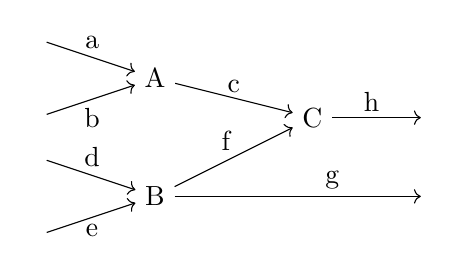
\begin{tikzpicture}
      [scale=.5, auto=center]
      \node (a) at (0,5) {};
      \node (b) at (0,3) {};
      \node (d) at (0,2) {};
      \node (e) at (0,0) {};
      \node (h) at (10,3) {};
      \node (A) at (3,4) {A};
      \node (B) at (3,1) {B};
      \node (C) at (7,3) {C};
      \node (g) at (10,1) {};
      \node (a_1) at (1.4,4.9) {a};
      \node (b_1) at (1.4,3) {b};
      \node (d_1) at (1.4,2) {d};
      \node (e_1) at (1.4,0.14) {e};
      \node (c_1) at (5,3.8) {c};
      \node (f_1) at (4.8,2.4) {f};
      \node (g_1) at (7.5,1.4) {g};
      \node (h_1) at (8.5,3.4) {h};
      \draw[->]
          (a) edge (A) (b) edge (A) (d) edge (B) (e) edge (B) (A) edge (C) (C) edge (h) (B) edge (g) (B) edge (C); 
  \end{tikzpicture}
  \end{center}
  where the "inputs" at each node are covectors and the "outputs" are vectors. Therefore, the entire diagram, which represents the tensor $X$ has a total of 4 inputs (indices $a, b, d, e$) and two outputs (indices $h, g$). We can see from the diagram that the indices $c$ and $f$, which travels "between" the factors are the ones that are being contracted. Therefore, the contraction of $c$ and $f$ contracts the rank (4,6) tensor $A \otimes B \otimes C$ to a rank (2,4) tensor. 
  \end{definition}

  \begin{definition}
  The \textbf{tensor algebra} of vector space $V$ over field $\mathbb{F}$ is an associative, noncommutative algebra defined
  \begin{align*}
      T(V) \equiv \bigoplus_{n = 0}^{\infty} V^{\otimes n} & = V^{\otimes 0} \oplus V^{\otimes 1} \oplus V^{\otimes 2} \oplus V^{\otimes 3} \oplus ... \\
      & = \mathbb{F} \oplus V \oplus V^{\otimes 2} \oplus V^{\otimes 3} \oplus V^{\otimes 4} \oplus ...
  \end{align*}
  with elements being infinite-tuples
  \[ (a, B^\mu, C^{\nu \gamma}, D^{\alpha \beta \epsilon}, ...)\]
  The addition operation is defined component-wise, and the multiplication operation is the tensor product 
  \[\otimes: T(V) \times T(V) \longrightarrow T(V)\]
  and the identity element is
  \[I = (1, 0, 0, ...) \]
  Linearity is easily proved. 
  \end{definition}

  The tensor algebra is used to "add" differently ranked tensors together. In order to do this rigorously, we must define the map (which is also an isomorphism)
  \[i_j: V^{\otimes j} \longrightarrow T(V), \; i_j (T^{\kappa_1, ..., \kappa j}) = (0, ...,0, T^{\kappa_1, ..., \kappa j}, 0, ..., 0) \]
  So, we can implicitly define the addition of arbitrary tensors $A \in V^{\otimes n}$ and $B \in V^{\otimes m}$ as 
  \[ A + B \equiv i_n (A) + i_m (B) \in T(V)\]
  along with the tensor multiplication of the form
  \[ A \otimes B \equiv i_n(A) \otimes i_m(B) \equiv i_{n+m} (A \otimes B)\]
  This allows us to alternatively define the tensor product operation as
  \[i_i(V^{\otimes i}) \otimes i_j( V^{\otimes j}) \equiv i_{i+j} (V^{\otimes (i+j)})\]

\subsection{Exterior Algebras and Symmetric Algebras}

  We can define the symmetric and exterior algebras multiple ways. In here, we will construct their powers separately as quotient spaces and direct sum them to create their respective algebras. But first, we must introduce the Schmidt decomposition, which is the foundation of all the results of this section. 

  \begin{theorem}[Schmidt Decomposition]
  For any $w \in U \otimes V$, where $U, V$ ($\dim{U} = n, \dim{V} = m$)  are inner product spaces over $\mathbb{F} \in \{ \mathbb{R}, \mathbb{C}\}$, there exists an orthonormal basis $\{u_i\}$ of $U$ and $\{v_j\}$ of $V$ such that 
  \[ w = \sum_{i=1}^{\min{\{n, m\}}} \alpha_i u_i \otimes v_i, \; \alpha_i \in \mathbb{F}\]
  \end{theorem}
  \begin{proof}
  Since $U \otimes V \simeq $ Hom$(V^*, U)$, we can interpret $w$ as a matrix $\Tilde{w}$. Using singular value decomposition, there exists unitary matrices $A, B$ and diagonal matrix $\Sigma$ such that
  \[\Tilde{w} = A \Sigma B^\dagger\]
  $C(A)$ and $R(B^\dagger)$ determine the orthonormal basis of $U \otimes V$, and we can thus see that the minimum number of required $u \otimes v$'s is precisely the number of nonzero singular values, which is the rank of $\Tilde{w}$. 

  \end{proof}

  \begin{definition}
  Let $I$ be a subspace of $V \otimes V$ generated by elements of the form $x \otimes x \in V \otimes V$. That is, given a basis $\{e_i\}$ of $n$-dimensional space $V$, all tensors of the form $x \otimes x \in V \otimes V$ can be written 
  \[x \otimes x = \sum_{i=1}^n a_i (e_i \otimes e_i) + \sum_{i \neq j} b_{i j} (e_i \otimes e_j + e_j \otimes e_i)\]
  which implies that the components of $e_i \otimes e_j$ and $e_j \otimes e_i$ must be the same for every element in $I$. 
  \end{definition}

  \begin{example}
  Given that $V$ is 2-dimensional, a vector $x \in V$ can be written $x = a e_1 + b e_2$, which implies
  \begin{align*}
      x \otimes x & = (a e_1 + b e_2) \otimes (a e_1 + b e_2) \\
      & = a^2 (e_1 \otimes e_1) + a b (e_1 \otimes e_2) + b a (e_2 \otimes e_1) + b^2 (e_2 \otimes e_2) \\
      & = a^2 (e_1 \otimes e_1) + b^2 (e_2 \otimes e_2) + a b (e_1 \otimes e_2 + e_2 \otimes e_1) 
  \end{align*}
  \end{example}

  Since we can group the components $e_i \otimes e_j$ and $e_j \otimes e_i$ together to $e_i \otimes e_j + e_j \otimes e_i$, the basis of $I$ is 
  \[\{e_1 \otimes e_1, ..., e_n \otimes e_n, e_1 \otimes e_2 + e_2 \otimes e_1, ..., e_{n-1} \otimes e_n + e_n \otimes e_{n-1}\}\]

  \begin{definition}
  Now, we can define the \textbf{second exterior power of $V$} as
  \[\Lambda^2 V \equiv \frac{V \otimes V}{I}\]
  and it follows that 
  \[\dim{\Lambda^2 V} = n^2 - \dim{I} = \frac{1}{2} n (n-1)\]
  We denote the elements of $\Lambda^2 V$ as $x \wedge y$, which really just represents the equivalence class of $x \otimes y$ in the quotient space. It is clear that $x \otimes x \in I \implies x \wedge x = 0$, so
  \begin{align*}
      0 = (x + y) \wedge (x + y) & = x \wedge x + x \wedge y + y \wedge x + y \wedge y \\
      & = x \wedge y + y \wedge x \\
      \implies & x \wedge y = - y \wedge x
  \end{align*}
  That is, the wedge product is antisymmetric. Note also that we can assume distributivity of $\wedge$ since it is just the quotient operation of another operation $\otimes$ that satisfies distributivity. We can construct a basis on $\Lambda^2 V$, given by 
  \[\{e_i \wedge e_j \; | \; i < j\}\]
  Again, we note that $i < j$ since $e_i \wedge e_i = 0$ and $e_i \wedge e_j = - e_j \wedge e_i$. 
  \end{definition}

  One realization of the space $\Lambda^2 \mathbb{R}^n$ is the set of antisymmetric $n \times n$ matrices. We can construct higher order exterior powers, too. For $n = 3$ (and assuming that $\dim{V} \geq 3$), the subspace $I \subset V \otimes V \otimes V$ is the space generated by elements of the forms
  \[x \otimes x \otimes y, x \otimes y \otimes x, y \otimes x \otimes x\]
  Following a similar construction, the \textbf{third exterior power of $V$} is
  \[\Lambda^3 V \equiv \frac{V \otimes V \otimes V}{I}\]
  with its elements being equivalence classes of the form
  \[x \wedge y \wedge z,\; x, y, z \in V\]
  such that
  \begin{align*}
      x \wedge y \wedge z & = - x \wedge z \wedge y \\
      & = - y \wedge x \wedge z \\
      & = - z \wedge y \wedge x
  \end{align*}
  The basis of $\Lambda^3 V$ is
  \[\{e_i \wedge e_j \wedge e_k \; | \; i < j < k\} \implies \dim{\Lambda^3 V} = \frac{1}{6} n (n-1) (n-2)\]
  Generally, if $\sigma$ is a permutation of the ordered list $(1, 2, ..., n)$, and $x_1, x_2, ..., x_n \in V$, then 
  \[x_{\sigma(1)} \wedge x_{\sigma(2)} \wedge ... \wedge_{\sigma(n)} = sgn(\sigma) \; x_1 \wedge x_2 \wedge ... \wedge x_n\]
  which means that if $x_i = x_j$ for some $1 \leq i \neq j \leq n$, 
  \[x_1 \wedge x_2 \wedge ... \wedge x_n = 0\]
  By constructing all the exterior powers of $n$-dimensional space $V$, we can construct the algebra 
  \begin{align*}
      \Lambda(V) \equiv \bigoplus_{k=0}^n \Lambda^k V \equiv \Lambda^0 V \oplus \Lambda^1 V \oplus \Lambda^2 V \oplus ... \oplus \Lambda^n V 
  \end{align*}
  Note that $\Lambda^0 V = \mathbb{F}$ and $\Lambda^1 V = V$. Unlike the tensor algebra, the exterior algebra is finite since the exterior powers vanish for finite $n$. In fact, 
  \[ \dim{\Lambda^k V} = \begin{cases}
  _n C_k & 0 \leq k \leq n \\
  0 & n < k
  \end{cases}\]
  which implies that 
  \[\dim{\Lambda(V)} = 2^n \]
  \begin{definition}
  The $n$th exterior power $\Lambda^n V$ is 1 dimensional, spanned by the singular basis vector 
  \[e_1 \wedge e_2 \wedge ... \wedge e_{n-1} \wedge e_n\]
  This vector is the \textit{determinant}. Note that this construction of the determinant is consistent with our previous construction of the determinant of a matrix since $e_1 \wedge ... \wedge e_n$ is indeed multilinear and antisymmetric. In its purest sense, 
  \[e_1 \wedge ... \wedge e_n: \prod_{i=1}^n V^* \longrightarrow \mathbb{F}\]
  is a mapping that is multilinear and antisymmetric. But there is an inconsistency. The matrix determinant takes in \textit{matrices} rather than taking in $n$-tuples of covectors. However, we can interpret the $n$ covectors in $V^* \times ... \times V^*$ as the column (or row) vectors of an $n \times n$ matrix. This completes the realization, and so we can conclude that the matrix determinant is just a realization of the more abstract determinant $e_1 \wedge ... \wedge e_n$. 

  Note that any tensor in $\Lambda^n V$ satisfies multilinearity and antisymmetricity, but only the basis vector $e_1 \wedge ... \wedge e_n$ satisfies the normalizing condition
  \[\det{I} = 1\]
  Since, given that the dual basis of $V^*$ is $\{f_j\}$
  \[(e_1 \wedge ... \wedge e_n) (f_1, f_2, ..., f_n) = \prod_{i=1}^n e_i (f_i) = \prod_{i=1}^n \delta_i^i = 1\]
  \end{definition}

  \begin{example}
  Given 3 dimensional vector space $V$ with basis $\{e_1, e_2, e_3\}$, the wedge product of two vectors $a, b \in V$ is 
  \begin{align*}
      a \wedge b & = (a_1 e_1 + a_2 e_2 + a_3 e_3) \wedge (b_1 e_1 + b_2 e_2 + b_3 e_3) \\
      & = (a_2 b_3 - a_3 b_2) e_2 \wedge e_3 + (a_3 b_1 - a_1 b_3) e_3 \wedge e_1 + (a_1 b_2 - a_2 b_1) e_1 \wedge e_2 
  \end{align*}
  which is essentially the formula for the cross product $\times$ in Euclidean space. We can therefore think of the realization of the wedge product in 3 dimensional space $V$ as the cross product. 
  \[\wedge: V \times V \longrightarrow \Lambda^2 V\]
  Note that $\Lambda^2 V \simeq V$ if $\dim{V} = 3$, so we can construct the more familiar $\times$ operation in $\mathbb{R}^3$. 
  \[\times: \mathbb{R}^3 \times \mathbb{R}^3 \longrightarrow \Lambda^2 \mathbb{R}^3 \simeq \mathbb{R}^3\]
  which is consistent with $\times$ taking two vectors and outputting a third vector living in $\mathbb{R}^3$ that is orthogonal to the two input vectors. 
  \end{example}

  \begin{example}
  The realization of the wedge product of 3 vectors in 3 dimensional space $V$ is the \textit{triple scalar product}, which we will denote as $\times_3$
  \[\wedge: V \times V \times V \longrightarrow \Lambda^3 V\]
  Note that since $\Lambda^3 V \simeq V$ when $\dim{V} = 3$, we can write 
  \[\times_3: \mathbb{R}^3 \times \mathbb{R}^3 \times \mathbb{R}^3 \longrightarrow \Lambda^3 \mathbb{R}^3 \simeq \mathbb{R}\]
  which is consistent with $\times_3$ taking three vectors and outputting the signed volume of their parallelopiped which lies in $\mathbb{R}$. 
  \end{example}

  Now we introduce the symmetric algebra and its construction. Let $I$ be the subspace of $V \otimes V$ generated by all tensors of the form 
  \[u \otimes v - v \otimes u, \; u, v \in V\]
  For example, given $a, b \in V$ with basis $\{e_1, e_2\}$, 
  \begin{align*}
      a \otimes b - b \otimes a & = (a_1 e_1 + a_2 e_2) \otimes (b_1 e_1 + b_2 e_2) - (b_1 e_1 + b_2 e_2) \otimes (a_1 e_1 + a_2 e_2) \\
      & = (a_1 b_2 - b_2 a_1) e_1 \otimes e_2 + (a_2 b_1 - b_2 a_1) e_2 \otimes e_1 
  \end{align*}
  is an element of $I$. We can generalize this to see that
  \[\{e_i \otimes e_j - e_j \otimes e_i\}, \; i \neq j\]
  is the basis for $I$. Now, let us define the \textit{second symmetric power of $V$} as 
  \[\Sym^2 V \equiv \frac{V \otimes V}{I}\]
  where, given that $\dim{V} = n$, 
  \[\dim{\Sym^2 V} = n^2 - \frac{1}{2} n (n-1) = \frac{1}{2} n (n+1)\]
  We denote the elements of $\Sym^2 V$ as $x \odot y$, which are really the equivalence classes $\{x \otimes y - y \otimes x\}$. Note that
  \begin{align*}
      x \odot y - y \odot x & = \{x \otimes y - y \otimes x\} - \{ y \otimes x - x \otimes y\} \\
      & = \{ x \otimes y - y \otimes x - y \otimes x + x \otimes y\} \\
      & = \{0\} = 0
  \end{align*}
  $\implies x \odot y = y \odot x$. That is, the $\odot$ operator is symmetric, and $\Sym^2 V$ has basis 
  \[ \{e_i \odot e_j\}_{j \geq k}\]
  One realization of $\Sym^2 \mathbb{R}^n$ is the set of all symmetric $n \times n$ real matrices. We can construct higher symmetric powers satisfying this property that its tensors are invariant under transpositions. 
  \[x_1 \odot ... x_i \odot ... x_j \odot ... x_n = x_1 \odot ... x_j \odot ... x_i \odot ... x_n\]
  for all $1 \leq i \neq j \leq n$, which implies that it is invariant under any permutation $p \in S_n$ of the $x_i$'s. Additionally, 
  \[\dim{\Sym^k V} = \binom{n+k-1}{k}\]

  \begin{definition}
  The \textbf{symmetric algebra} of vector space $V$ is constructed as such 
  \[\Sym (V) \equiv \bigoplus_{k=0}^\infty \Sym^k V\]
  Note that unlike the exterior algebra, $\Sym(V)$ is infinite dimensional. 
  \end{definition}

  \begin{example}
  The inner product $(\cdot, \cdot)$ on $V$ is an element of $\Sym^2 V$, since it is a bilinear, symmetric operation on $V$. 
  \[\odot, (\cdot, \cdot): V \times V \longrightarrow \mathbb{F}\]
  \end{example}

  There is a simple relationship between $V \otimes V$, $\Lambda^2 V$, and $\Sym^2 V$. 

  \begin{theorem}
  \[V \otimes V \simeq \Sym^2 V \oplus \Lambda^2 V\]
  with isomorphism defined
  \[v \otimes w \mapsto \Big( \frac{1}{2} (v \odot w), \frac{1}{2} (v \wedge w) \Big)\]
  This is precisely the factoring of a rank (2,0) tensor into its symmetric and antisymmetric parts. 
  \end{theorem}
  \begin{proof}
  Given $v \otimes w \in V \otimes V$, 
  \[v \otimes w + w \otimes v \in \Sym^2 V \text{ and } v \otimes w - w \otimes v \in \Lambda^2 V\]
  By defining $v \odot w$ and $v \wedge w$ as the expressions above, the isomorphism is satisfied. 
  \end{proof}

  Therefore, when working in $V \otimes V$, we can interpret 
  \begin{align*}
      & v \wedge w = \frac{1}{2} (v \otimes w - w \otimes v) \\
      & v \odot w = \frac{1}{2} (v \otimes w + w \otimes v) 
  \end{align*}

  However, 
  \[V \otimes V \otimes V \not\simeq \Sym^3 V \oplus \Lambda^3 V\]
  \textit{Schur functors} are used to fix this discrepancy. 

  Note that we have introduced these two algebras by first constructing the quotient spaces $\Lambda^n V$ and $\Sym ^n V$ from the tensor product spaces $T^{\otimes n}$ and then direct summing these powers to construct the algebras. We will introduce another type of construction that directly takes the quotient algebra of $T(V)$ with the two-sided ideal. 


\section{Exercises} 

\subsection{Group Like Structures}

  \begin{exercise}[Math 401 Spring 2025 Midterm 2]
    Listed. 
    \begin{enumerate}
      \item Let $G$ be a finite group with an even number of elements. Show that $G$ contains an element of order $2$. 
      \item Prove that a group of order $10$ contains an element of order $5$. 
    \end{enumerate}
  \end{exercise}
  \begin{solution}
    Listed. 
    \begin{enumerate}
      \item We know that $e^{-1} = e$, and so remove it from $G$. Then $G$ has an odd number of elements. Now as long as $G$ is nonempty, we can remove $a, a^{-1}$, resulting in an odd cardinality. Since $G$ is finite, this must terminate, and so there must be a case where $a = a^{-1} \implies \ord(a) = 2$. 
      \item Assume that there is no element of order $5$. Then from above it must contain an element of order $2$, and let us call it $a \in G$. $\ord(e) = 1$ obviously. If any $b \in G$ had order 10, then $G = Z_{10}$, which would mean that $\ord(b^5) = 2$. Therefore every element other than the identity must have order $2$. But then given $a, b, ab \in G$, $ab \neq a, b$ since $ab = a \implies b = e$, and this is precisely the Klein 4 group. This subgroup has an order that doesn't divide 10, contradicting Lagrange's theorem. 
    \end{enumerate}
  \end{solution}

  \begin{exercise}[Shifrin 6.1.1]
    Which of the following are groups?
    \begin{enumerate}
      \item[(a)] $\{1,3,7,9\} \subset \mathbb{Z}_{10}$, with operation multiplication
      \item[(b)] $\{0,2,4,6\} \subset \mathbb{Z}_{10}$, with operation addition
      \item[(c)] $\{x \in \mathbb{Q} : 0 < x \leq 1\}$, with operation multiplication
      \item[(d)] the set of all positive irrational real numbers, with operation multiplication
      \item[(e)] the set of imaginary numbers $ix, x \in \mathbb{R}$, with operation addition
      \item[(f)] the set of complex numbers of modulus 1, with operation multiplication
      \item[(g)] $\mathbb{Z}$ with operation $a \bullet b = a + b + 1$
      \item[(h)] $\mathbb{Z}$ with operation $a \bullet b = a - b$
      \item[(i)] $\mathbb{Q} - \{1\}$ with operation $a \bullet b = a + b - ab$
    \end{enumerate}
  \end{exercise}
  \begin{solution}
    Listed. We will denote the sets in question to be $G$. 
    \begin{enumerate}
      \item[(a)] Is a group since product of 2 odds is odd, so is closed. Also we have $1$ as the identity with $3^{-1} = 7, 7^{-1} = 3, 9^{-1} = 9$. It is associative since multiplication on $\mathbb{Z}_{10}$ is associative. 
      \item[(b)] Not a group since $4 + 4 = 8 \not\in G$. 
      \item[(c)] Not a group since $1/2 \in G$ but $(1/2)^{-1} = 2 \not\in G$. 
      \item[(d)] Not a group since $\sqrt{2} \times \sqrt{2} 2  \not\in G$. 
      \item[(e)] Is a group since identity is $0 = 0i$, $ix + iy = i (x + y)$ with $x + y \in \mathbb{R}$, and $-(ix) = i (-x)$ where $-x \in \mathbb{R}$. 
      \item[(f)] Is a group since this is a representation of $O(2)$. 
      \item[(g)] Is a group since this is obviously closed under $\mathbb{Z}$ since $+_{\mathbb{Z}}$ is closed. Now assume that $i$ is the identity. Then $a \bullet i = a + i + 1 = a \implies i = -1$. Therefore $a \bullet a^{-1} = a + a^{-1} + 1 = -1 \implies a^{-1} = -a - 2$. This is associative since 
      \begin{equation}
        (a \bullet b) \bullet c = (a + b + 1) \bullet c = a + b + c + 2 = a \bullet (b + c + 1) = a \bullet (b \bullet c)
      \end{equation}
      \item[(h)] Not a group since it is not associative. Note $(a \bullet b) \bullet c = (a - b) \bullet c = a - b - c$, while $a \bullet (b \bullet c) = a \bullet (b - c) = a - b + c$. 
      \item[(i)] Is a group. We claim that it is closed. Assume not; given $a, b \neq 1$, 
        \begin{equation}
          a \bullet b = a + b - ab = 1 \implies 0 = ab - a - b + 1 = (a - 1)(b-1) 
        \end{equation}
        which means $a = 1$ or $b = 1$, which is a contradiction. As for the identity, $a \bullet i = a + i - ai = a \implies 0 = i - ai = i (1 - a) \implies i = 0$ since $a \neq 1$. We can define the inverse by solving 
        \begin{equation}
          0 = a \bullet a^{-1} = a + a^{-1} - a a^{-1} \implies a^{-1} (1 - a) = -a \implies a^{-1} = \frac{a}{a-1}
        \end{equation}
        which is well-defined since $a \neq 1$. Finally, it is associative since 
        \begin{align}
          (a \bullet b) \bullet c & = (a + b - ab) \bullet c \\
                                  & = a + b - ab + c - ac - bc - abc \\
                                  & = a + b + c - bc - ab - ac - abc \\
                                  & = a \bullet (b + c - bc) \\
                                  & = a \bullet (b \bullet c)
        \end{align}
    \end{enumerate}
  \end{solution}

  \begin{exercise}[Shifrin 6.1.10]
    \begin{enumerate}
      \item[(a)] Let $G$ be a group. Prove that $(ab)^2 = a^2b^2$ for all $a,b \in G$ if and only if $G$ is abelian.
      \item[(b)] Prove that if every element (other than the identity element) of a group $G$ has order 2, then $G$ is abelian.
    \end{enumerate}
  \end{exercise}
  \begin{solution}
    For (a), if $G$ is abelian, then 
    \begin{equation}
      (ab)^2 = (ab) (ab) = a (ba) b = a (ab) b = (aa) (bb) = a^2 b^2
    \end{equation}
    If the identity holds, then 
    \begin{equation}
      (ab)^2 = a^2 b^2 \implies (a^{-1} a) (ba) (b b^{-1}) = a^{-1} (ab)(ab) b^{-1} = a^{-1} a^2 b^2 b^{-1} \implies ba = ab
    \end{equation} 
    For (b), since we have $a^2 = e, b^2 = e$, and $(ab)^2 = e$, from (a) $G$ is abelian. 
  \end{solution}

  \begin{exercise}[Shifrin 6.1.17]
    \begin{enumerate}
      \item[(a)] A group has four elements $a$, $b$, $c$, and $d$, subject to the rules $ca = a$ and $d^2 = a$. Fill in the entire multiplication table at the left below.
      
      \begin{tabular}{c|cccc}
        $\cdot$ & $a$ & $b$ & $c$ & $d$ \\
        \hline
        $a$ & & & & \\
        $b$ & & & & \\
        $c$ & $a$ & & & \\
        $d$ & & & & $a$ \\
      \end{tabular}
      
      \item[(b)] A group has six elements $a$, $b$, $c$, $d$, $e$, and $f$, subject to the rules $ae = a$, $bd = a$, $c^2 = a$, and $df = a$. Fill in the entire multiplication table at the right above.
      
      \begin{tabular}{c|cccccc}
        $\cdot$ & $a$ & $b$ & $c$ & $d$ & $e$ & $f$ \\
        \hline
        $a$ & & & & & $a$ & \\
        $b$ & & & & $a$ & & \\
        $c$ & & & $a$ & & & \\
        $d$ & & & & & & $a$ \\
        $e$ & & & & & & \\
        $f$ & & & & & & \\
      \end{tabular}
    \end{enumerate}
  \end{exercise}
  \begin{solution}
    We can see that $ca = a \implies c = ca a^{-1} = a a^{-1} = i$, so $c$ is the identity. We can fill in the row and column of $c$. Then, we can figure out what $bd$ is. It cannot be $b$ or $d$ since $c$ is the unique identity, so it must be either $a$ or $c$. It cannot be $a$ since then $bd = a = d^2$, and so $b = d$. So it must be $c$. By the same logic we can fill out the rest of the rows and columns. 

    \begin{tabular}{c|cccc}
      $\cdot$ & $a$ & $b$ & $c$ & $d$ \\
      \hline
      $a$ & $c$ & $d$ & $a$ & $b$ \\
      $b$ & $d$ & $a$ & $b$ & $c$ \\
      $c$ & $a$ & $b$ & $c$ & $d$ \\
      $d$ & $b$ & $c$ & $d$ & $a$ \\
    \end{tabular}

    By the same logic as the previous, we can immediately see that $ae = a \implies e$ is the identity. The formal logic above can be simplified down to saying that there can be no two of the same elements in the same row or column, since if it were, then we are saying that $xy = xz \implies y = z$, which cannot be the case since $y$ and $z$ are distinct. So $fb = a$. We can also deduce that $da = ab$ and $ba = af$. At this point, we can recognize that this is the Dihedral group of order $6$, and so we fill in the rest of the multiplication table. 

    \begin{tabular}{c|cccccc}
      $\cdot$ & $a$ & $b$ & $c$ & $d$ & $e$ & $f$ \\
      \hline
      $a$ & c & f & e & b & a & d \\
      $b$ & d & e & f & a & b & c \\
      $c$ & e & d & a & f & c & b \\
      $d$ & f & c & b & e & d & a \\
      $e$ & a & b & c & d & e & f \\
      $f$ & b & a & d & c & f & e
    \end{tabular}
  \end{solution}

\subsection{Subgroups and Quotient Groups}

  \begin{exercise}[Shifrin 6.2.2]
    Prove that $\mathbb{Z}_7^{\times} \cong \mathbb{Z}_6$. (It is crucial to remember that we multiply in $\mathbb{Z}_7^{\times}$ and add in $\mathbb{Z}_6$.)
  \end{exercise}
  \begin{solution}
    Both groups are of order 6, and so $\mathbb{Z}_7^\times$---which is indeed a group (since it is the group of units of the ring $(\mathbb{Z}_7, +, \times)$)---must be isomorphic to either $\mathbb{Z}_6$ or $S_3$. However, $S_3$ is not abelian, while $\mathbb{Z}^\times_7$ is, so it must be the case that it is isomorphic to $\mathbb{Z}_6$. 
  \end{solution}

  \begin{exercise}[Shifrin 6.2.15.a/b]
    The \textbf{dihedral group} of order $2n$, denoted $\mathcal{D}_n$, is given by $\{\rho^i\psi^j : 0 \leq i < n, 0 \leq j \leq 1\}$ subject to the rules $\rho^n = e$, $\psi^2 = e$, and $\psi\rho\psi^{-1} = \rho^{-1}$.
    \begin{enumerate}
      \item Check this is really a group. That is, what is $(\rho^i\psi^j)^{-1}$, and what is the product $(\rho^i\psi^j)(\rho^k\psi^\ell)$?
      \item Check that $\mathcal{T} \cong \mathcal{D}_3$ and $S_q \cong \mathcal{D}_4$.
    \end{enumerate}
  \end{exercise}
  \begin{solution}
    We check the properties of a group. The following identity is useful: 
    \begin{equation}
      (\psi \rho \psi^{-1})^{n-i} = (\rho^{-1})^{n-i} \implies \psi \rho^{n-i} \psi^{-1} = \rho^i \implies \psi \rho^{n-i} = \rho^i \psi
    \end{equation}
    \begin{enumerate}
      \item \textit{Closure}. From simplifying according to the first two rules, we will automatically adjust the exponents to be $i, k < n$ (by subtracting out multiples of $n$) and $j \in \{0, 1\}$ (by subtracting out multiples of $2$). Going case by case, 
      \begin{enumerate}
        \item $j = 0, l = 0$. $\rho^i \rho^k = \rho^{i+k}$. 
        \item $j = 0, l = 1$. $\rho^i \rho^k \psi = \rho^{i+k} \psi$. 
        \item $j = 1, l = 0$. $\rho^i \psi \rho^k = \rho^i \rho^{n-k} \psi = \rho^{n-k+i} \psi$. 
        \item $j = 1, l = 1$. $\rho^i \psi \rho^k \psi = \rho^i \psi \psi \rho^{n-k} = \rho^i \rho^{n-k} = \rho^{n-k+i}$. 
      \end{enumerate}
      \item \textit{Identity}. The identity is $e = \rho^0 \psi^0$. We can see that $e \rho^i \psi^j = \rho^i \psi^j e = \rho^{i+0} \psi^j$. 
      \item \textit{Inverse}. We have $\psi \rho \psi^{-1} = \psi \rho \psi = \rho^{-1} \implies \psi \rho = \rho^{-1} \psi^{-1} = (\psi \rho)^{-1}$. Therefore, 
      \begin{equation}
        (\rho^i \psi^j)^{-1} = \begin{cases} 
          \rho^{n - i} & \text{ if } j = 0  \\
          \rho^{i} \psi & \text{ if } j = 1
        \end{cases}
      \end{equation}
      which are both of the correct form and therefore in $\mathcal{D}_n$. To verify, we see that $\rho^i \rho^{n-i} = \rho^n = e$, and $(\rho^i \psi) (\rho^i \psi) = \rho^i \psi \psi \rho^{n-i} = \rho^i \rho^{n-i} = e$.  
      \item \textit{Associativity}. Can also be proven tediously but problem only asked to state the product and inverse.  
    \end{enumerate} 

    For (b) for $\mathcal{T}$, we can explicitly look at the multiplication tables and see that they are isomorphic. We denote $r_1, r_2$ as the 120 and 240 degree rotations, and $f_1, f_2, f_3$ as the flips across each axis. 

    \begin{figure}[H]
      \centering
      \begin{subfigure}[b]{0.48\textwidth}
        \centering
        \begin{tabular}{c|cccccc}
          & $e$ & $\rho$ & $\rho^2$ & $\psi$ & $\rho\psi$ & $\rho^2\psi$ \\
          \hline
          $e$ & $e$ & $\rho$ & $\rho^2$ & $\psi$ & $\rho\psi$ & $\rho^2\psi$ \\
          $\rho$ & $\rho$ & $\rho^2$ & $e$ & $\rho^2\psi$ & $\psi$ & $\rho\psi$ \\
          $\rho^2$ & $\rho^2$ & $e$ & $\rho$ & $\rho\psi$ & $\rho^2\psi$ & $\psi$ \\
          $\psi$ & $\psi$ & $\rho^2\psi$ & $\rho\psi$ & $e$ & $\rho^2$ & $\rho$ \\
          $\rho\psi$ & $\rho\psi$ & $\psi$ & $\rho^2\psi$ & $\rho$ & $e$ & $\rho^2$ \\
          $\rho^2\psi$ & $\rho^2\psi$ & $\rho\psi$ & $\psi$ & $\rho^2$ & $\rho$ & $e$
        \end{tabular}
        \caption{$\mathcal{D}_3$}
      \end{subfigure}
      \hfill 
      \begin{subfigure}[b]{0.48\textwidth}
        \centering
        \begin{tabular}{c|cccccc}
          & $e$ & $r_1$ & $r_2$ & $f_1$ & $f_2$ & $f_3$ \\
          \hline
          $e$ & $e$ & $r_1$ & $r_2$ & $f_1$ & $f_2$ & $f_3$ \\
          $r_1$ & $r_1$ & $r_2$ & $e$ & $f_3$ & $f_1$ & $f_2$ \\
          $r_2$ & $r_2$ & $e$ & $r_1$ & $f_2$ & $f_3$ & $f_1$ \\
          $f_1$ & $f_1$ & $f_2$ & $f_3$ & $e$ & $r_2$ & $r_1$ \\
          $f_2$ & $f_2$ & $f_3$ & $f_1$ & $r_1$ & $e$ & $r_2$ \\
          $f_3$ & $f_3$ & $f_1$ & $f_2$ & $r_2$ & $r_1$ & $e$
        \end{tabular}
        \caption{$\mathcal{T}$}
      \end{subfigure}
    \end{figure}

    For $S_q$, it is tedious to write the full table, so we construct the isormorphisms using the generators. For $S_q$, the symmetry group of the square consists of 8 elements: the 4 rotations $r_1, r_2, r_3, r_4$ (of 90, 180, 270, and 360=0 degrees), and the flips $f_1, f_2, f_3, f_4$ (across each axis). Now we construct the function $g: \mathcal{D}_3 \rightarrow \mathcal{T}$ such that $f(\rho) = r_1$ and $f(\psi) = f_1$. Then we can see that 
    \begin{equation}
      g(\rho^4) = g(e) = e = r_1^4 = g(\rho^4), \qquad g(\psi^2) = g(e) = e = f_1^2 = g(\psi)^2
    \end{equation}
    since 90 degrees rotated 4 times is $0$ degrees, the identity, and two flips across the same axis is also the identity. Finally, we have 
    \begin{equation}
      g(\psi \rho \psi) = g(\rho^{-1}) = r_1^{-1} = r_3 = f_1 r_1 f_1 = g(\psi) g(\rho) g(\psi)
    \end{equation}
    Where $r_1^{-1} = r_3$ since a rotation of 270 after a 90 is the same as rotation by 360=0, and $r_3 = f_1 r_1 f_1$ is the change of basis symmetry observed in Shifrin Example 6.1.5. Therefore the rules match, making it a homomorphism, and since the order is the same ($\mathcal{D}_3$ has $4 \times 2 = 8$ elements from looking at the indices), this is an isomorphism. 
  \end{solution}

  \begin{exercise}[Shifrin 6.3.8]
    Let $H \subset G$ be a subgroup, and let $a \in G$ be given. Prove that $aHa^{-1} \subset G$ is a subgroup (called a \textbf{conjugate subgroup} of $H$). Prove, moreover, that it is isomorphic to $H$ (cf. Exercise 6.2.12).
  \end{exercise}
  \begin{solution}
    Let $x, y \in aHa^{-1}$. Then $x = a h_x a^{-1}, y = a h_y a^{-1}$ for some $h_x, h_y \in H$. Therefore, 
    \begin{enumerate}
      \item It is closed. $xy = (a h_x a^{-1}) (a h_y a^{-1}) = a h_x (a^{-1} a) h_y a^{-1} = a h_x h_y a^{-1} \in aHa^{-1}$ since $h_x h_y \in H$ by closure. 
      \item It has an identity since $e \in H \implies a e a^{-1} = a a^{-1} = e \in aHa^{-1}$. 
      \item It has inverses since given $x \in H$ as above with inverses $x^{-1}$, we see that $(a x a^{-1})^{-1} = (a^{-1})^{-1} x^{-1} a^{-1} = a x^{-1} a^{-1} \in a H a^{-1}$ since $x^{-1} \in H$ by $H$ being a group. 
      \item Associativity is inherited from $G$. 
    \end{enumerate} 
    It suffices to show that this is injective, since the map $\iota : H \rightarrow a H a^{-1}$ is surjective by definition. Given $x, y \in a H a^{-1}$ with $x = y$, we have $a h_x a^{-1} = a h_y a^{-1}$, and multiplying by $a$ on the right and then $a^{-1}$ on the left, we get $h_x = h_y$.
  \end{solution}

  \begin{exercise}[Shifrin 6.3.11]
    Prove that a group of order $n$ has a proper subgroup if and only if $n$ is composite.
  \end{exercise}
  \begin{solution}
    We prove bidirectionally. Call the group $G$ and subgroup $H$. 
    \begin{enumerate}
      \item $(\rightarrow)$. Assume $n$ is prime. Then by Lagrange's theorem $|H|$ must divide $n$, and so $|H| = 1$ or $n$, neither of which results in a proper subgroup. 
      \item $(\leftarrow)$. Assume $G$ has a proper subgroup $H$. Since it is proper, $|H| \neq 1, n$. Then by Lagrange's theorem, $|H|$ divides $n$, which implies that $n$ is composite. 
    \end{enumerate}
  \end{solution}

  \begin{exercise}[Shifrin 6.3.13]
    Suppose $H, K \subset G$ are subgroups of orders $5$ and $8$, respectively. Prove that $H \cap K = \{e\}$.
  \end{exercise}
  \begin{solution}
    Let us take an arbitrary element in $x \in H \cap K$ and consider the cyclic group $\langle x \rangle$. By Lagrange's Theorem, the order $|x|$ in $H$ must be either $1$ or $5$, while the order in $K$ must be $1, 2, 4, 8$. Therefore, $|x| = 1$ and so $x = e$. 
  \end{solution}

  \begin{exercise}[Shifrin 6.3.17]
    \begin{enumerate}
      \item Prove that a group $G$ of even order has an element of order $2$. (Hint: If $a \neq e$, $a$ has order $2$ if and only if $a = a^{-1}$.)
      \item Suppose $m$ is odd, $|G| = 2m$, and $G$ is abelian. Prove $G$ has precisely one element of order $2$. (Hint: If there were two, they would provide a Klein four-group.)
      \item Prove that if $G$ has exactly one element of order $2$, then it must be in the center of $G$.
    \end{enumerate}
  \end{exercise}
  \begin{solution}
    Listed. 
    \begin{enumerate}
      \item Assume the contrary and take $H = G \setminus \{e\}$. Then $|H|$ is odd, and since no element has order $2$, every element must be associated with a unique inverse $a, a^{-1}$. But this cannot happen since $|H|$ is odd. Therefore there must be at least one element of order $2$. 

      \item It has at least 1 element of order 2 from (1). Now assume that there are two, call them $a, b$. Then $ab \neq a, b$ and $ab$ also has order $2$ since $(ab)(ab) = abba = aa = e$. Therefore, calling $c = ab$, we have $ac = ca = aab = b$ and $bc = cb = abb = a$. This fully defines the multiplication table for the Klein 4 group $K$ of order $4$. Therefore, by Lagrange's theorem, we have found a subgroup $K$ and so $|K|$ must divide $G$. However, this would mean that $m$ must be even, a contradiction. Therefore there is only one such unique $a$. 

      \item Given $a \in G$ with $|a| = 2$, we wish to show that it is an element of $Z = \{ b \in G \mid bx = xb \forall x \in G\}$.\footnote{I am using the definition of center defined in Shifrin 6.3.7.} Consider $z = x^{-1} a x$. We have 
      \begin{equation}
        z^2 = (x^{-1} a x)^2 = x^{-1} a x x^{-1} a x = x^{-1} a^2 x = x^{-1} x = e
      \end{equation}
      which means that $z$ also has order $2$. But since this is unique, it must be that $z = a$. Therefore, by multiplying $x$ on the left, we get 
      \begin{equation}
        x^{-1} a x = a \implies ax = xa
      \end{equation}
    \end{enumerate}
  \end{solution}
  
  \begin{exercise}[Assigned]
    Find all group homomorphisms $\mathbb{Z}_n \to \mathbb{Z}_m$. (Your answer will depend on $n$ and $m$.) 
  \end{exercise}
  \begin{solution}
    Given a homomorphism, $f$, we must have $f(0) = 0$. Let $f(1) = k$. Note that the value of $f(1) = k$ completely determines the homomorphism since the image of every other $l \in \mathbb{Z}_n$ is defined by 
    \begin{equation}
      f(l) = f(\underbrace{1 + \ldots + 1}_{l \text{ times}}) = \underbrace{k + \ldots + k}_{l \text{ times}}
    \end{equation}
    Since the image of $f$ must be a cyclic subgroup of $\mathbb{Z}_m$, we must satisfy 
    \begin{align}
      0 = f(0) & = f(\underbrace{1 + \ldots + 1}_{n \text{ times}}) \\
               & = \underbrace{k + \ldots + k}_{n \text{ times}} 
    \end{align}
    and so $m \mid nk$. Therefore, $k$ must be a multiple of $m/\gcd(n, m)$. So all homomorphisms are determined by the set 
    \begin{equation}
      \bigg\{ k = \frac{a m}{\gcd(n, m)} \; \bigg| \; a \in \mathbb{N}, 0 \leq k \leq m-1 \bigg\}
    \end{equation}
    which we can see ranges from $0 \leq a < \gcd(n, m)$, and so the total number of homomorphisms is $\gcd(n, m)$. Note that there is always the trivial homomorphism when $a = 0$, i.e. everything maps to $0$. For example, if we have $f: \mathbb{Z}_{14} \to \mathbb{Z}_{21}$, we have $k = 0, 3, 6, 9, 12, 15, 18$. 
  \end{solution}

\subsection{Group Actions}

\subsection{Product Groups}

\subsection{Ring Like Structures}

  \begin{exercise}[Shifrin 1.2.1]
    For each of the following pairs of numbers $a$ and $b$, find $d = \gcd(a,b)$ and express $d$ in the form $ma+nb$ for suitable integers $m$ and $n$.
    \begin{enumerate}
      \item[(a)] $14, 35$
      \item[(b)] $56, 77$
      \item[(c)] $618, 336$
      \item[(d)] $2873, 6643$
      \item[(e)] $512, 360$
      \item[(f)] $4432, 1080$
    \end{enumerate}
  \end{exercise}
  \begin{solution}
    Listed. 
    \begin{enumerate}
      \item $d = 7 = (-2) \cdot 14 + (1) \cdot 35$. 
      \item $d = 7 = (-4) \cdot 56 + 3 \cdot 77$. 
      \item $d = 6 = -25 \cdot 618 + 46 \cdot 336$ 
      \item $d = 13 = 37 \cdot 2873 + (-16) \cdot 6643$. 
      \item $d = 8 = 19 \cdot 512 + (-27) \cdot 360$. 
      \item $d = 8 = 29 \cdot 4432 + (-119) \cdot 1080$. 
    \end{enumerate}
  \end{solution}

  \begin{exercise}[Shifrin 1.2.2]
    You have at your disposal arbitrarily many 4-cent stamps and 7-cent stamps. What are the postages you can pay? Show in particular that you can pay all postages greater than 17 cents.
  \end{exercise}

  \begin{exercise}[Shifrin 1.2.3]
    Prove that whenever $m \neq 0$, $\gcd(0, m) = |m|$.
  \end{exercise}

  \begin{exercise}[Shifrin 1.2.4]
    \begin{enumerate}
      \item[(a)] Prove that if $a|x$ and $b|y$, then $ab|xy$.
      \item[(b)] Prove that if $d = \gcd(a, b)$, then $\gcd(\frac{a}{d}, \frac{b}{d}) = 1$.
    \end{enumerate}
  \end{exercise}

  \begin{exercise}[Shifrin 1.2.5]
    Prove or give a counterexample: the integers $q$ and $r$ guaranteed by the division algorithm, Theorem 2.2, are unique.
  \end{exercise}

  \begin{exercise}[Shifrin 1.2.6]
     Prove or give a counterexample. Let $a, b \in \mathbb{Z}$. If there are integers $m$ and $n$ so that $d = am + bn$, then $d = \gcd(a, b)$.
  \end{exercise}

  \begin{exercise}[Shifrin 1.2.7]
    Generalize Proposition 2.5: if $\gcd(m, c) = 1$ and $m|cz$, then prove $m|z$.
  \end{exercise}
  \begin{solution}
    Let $\mathrm{gcd}(m, c) = 1$ and $m | cz$. Then there exists $a, b \in \mathbb{Z}$ such that $am + bc = 1$. Multiply both sides of the equation by $z$ to get by the distributive property 
    \begin{equation}
      (am + bc) z = amz + bcz = z
    \end{equation} 
    $m | amz$ and $m | cz \implies m | bcz$. Therefore, the sum of the two, which is equal to $z$, must be divisible by $m$. Therefore $m | z$. 
  \end{solution}

  \begin{exercise}[Shifrin 1.2.8]
    Suppose $a, b, n \in \mathbb{N}$, $\gcd(a, n) = 1$, and $\gcd(b, n) = 1$. Prove or give a counterexample: $\gcd(ab, n) = 1$.
  \end{exercise}

  \begin{exercise}[Shifrin 1.2.9]
    Prove that if $p$ is prime and $p|(a_1 a_2 \ldots a_n)$, then $p|a_j$ for some $j$, $1 \leq j \leq n$. (Hint: Use Proposition 2.5 and induction.)
  \end{exercise}

  \begin{exercise}[Shifrin 1.2.10]
    Given a positive integer $n$, find $n$ consecutive composite numbers.
  \end{exercise}

  \begin{exercise}[Shifrin 1.2.11]
    Prove that there are no integers $m, n$ so that $(\frac{m}{n})^2 = 2$. (Hint: You may start by assuming $m$ and $n$ are relatively prime. Why? Then use Exercise 1.1.3.)
  \end{exercise}

  \begin{exercise}[Shifrin 1.2.12]
    Find all rectangles whose sides have integral lengths and whose area and perimeter are equal.
  \end{exercise}

  \begin{exercise}[Shifrin 1.2.13]
    Given two nonzero integers $a, b$, in analogy with the definition of $\gcd(a, b)$, we define the \textbf{least common multiple} $\operatorname{lcm}(a, b)$ to be the positive number $\mu$ with the properties:
    \begin{enumerate}
      \item[(i)] $a|\mu$ and $b|\mu$, and
      \item[(ii)] if $s \in \mathbb{Z}$, $a|s$ and $b|s \Rightarrow \mu|s$.
    \end{enumerate}
    Prove that
    \begin{enumerate}
      \item[(a)] if $\gcd(a, b) = 1$, then $\mu = ab$. (Hint: If $\gcd(a, b) = 1$, then there are integers $m$ and $n$ so that $1 = ma + nb$; therefore, $s = mas + nbs$.)
      \item[(b)] more generally, if $\gcd(a, b) = d$, then $\mu = ab/d$.
    \end{enumerate}
  \end{exercise}
  \begin{solution}
    Listed. 
    \begin{enumerate}
      \item We can simply verify the two properties. Since $\mu = ab$, $a | \mu$ and $b | \mu$ trivially by the existence of $b$ and $a$, respectively. As for the second property, let $s \in \mathbb{Z}$ exist such that $a | s$ and $b | s$. Since $a | s$, $s = xa$ for some $x \in \mathbb{Z}$. But since $b | s$, $b | xa$. Since $\mathrm{gcd}(a, b) = 1$ by assumption, the result in [Shifrin 1.2.7] tells us that $b | x$, i.e. there exists some $k \in \mathbb{Z}$ such that $x = kb$. Therefore $s = xa = kba = kab = k \mu$. By existence of $k$, $\mu | s$, and we are done. 
      \item Given $a, b$ with $\mathrm{gcd}(a, b) = d$, there exists some $a^\prime, b^\prime \in \mathbb{Z}$ s.t. $a = da^\prime, b = db^\prime$. We claim that $\mu = ab/d \coloneqq d a^\prime b^\prime$ is the lcm.\footnote{Since division isn't generally closed in the integers, I prefer to define $ab/d$ this way.} It is clear that $a | \mu$ and $b | \mu$ by the existence of integers $b^\prime$ and $a^\prime$, respectively. To prove the second property, let $s \in \mathbb{Z}$ with $a | s$ and $b | s$. Since $a | s \iff d a^\prime | s$, there must exist some $x \in \mathbb{Z}$ s.t. $s = d a^\prime x$. But since $b | s$, this means that $d b^\prime | s \iff d b^\prime | d a^\prime x \iff b^\prime | a^\prime x$. But $\mathrm{gcd}(a^\prime, b^\prime) = 1$ which follows from the definition of gcd, and so by [Shifrin 1.2.7] it must be the case that $b^\prime | x$, i.e. there exists some $k \in \mathbb{Z}$ s.t. $x = b^\prime k$. Substituting this back we have $s = d a^\prime b^\prime k = \mu k$, and by existence of $k$ it follows that $\mu | s$. Since it satisfies these 2 properties $\mu$ is the lcm. 
    \end{enumerate}
  \end{solution} 

  \begin{exercise}[Shifrin 1.2.14]
    See Exercise 13 for the definition of $\operatorname{lcm}(a, b)$. Given prime factorizations $a = p_1^{\mu_1} \cdots p_m^{\mu_m}$ and $b = p_1^{\nu_1} \cdots p_m^{\nu_m}$, with $\mu_i, \nu_i \geq 0$, express $\gcd(a, b)$ and $\operatorname{lcm}(a, b)$ in terms of $p_1,\ldots,p_m$. Prove that your answers are correct.
  \end{exercise}

  \begin{exercise}[Shifrin 1.3.8] 
    We see that in $\bmod{10}$, 
    \begin{align}
      3^{400} \equiv 9^{200} \equiv (-1)^{200} \equiv 1^{100} \equiv 1
    \end{align} 
    so the last digit is $1$. To get the last 2 digits, we use the binomial expansion and focus on the last 2 terms. 
    \begin{equation}
      3^{400} = 9^{200} = (10 - 1)^{200} = \ldots + \binom{200}{199} 10^1 (-1)^{199} + \binom{200}{200} (-1)^{200} 
    \end{equation}
    since every combination of the form $\binom{n}{k}$ is an integer and all the other terms have a factor of $10^2$, the expansion $\bmod{100}$ becomes 
    \begin{equation}
      3^{400} \equiv \binom{200}{199} 10^1 (-1)^{199} + \binom{200}{200} (-1)^{200} = 200 \cdot 10 \cdot (-1)^{199} + 1 \equiv 1 \pmod{100}
    \end{equation}
    and so the last two digits is $01$. To get the last digit of $7^{99}$, we see that in $\bmod{10}$, 
    \begin{equation}
      7^{99} \equiv 7^{96} \cdot 7^3 \equiv (7^4)^{24} \cdot 343 \equiv 2401^{24} \cdot 343 \equiv 1^{24} \cdot 3 \equiv 3
    \end{equation}
  \end{exercise}

  \begin{exercise}[Shifrin 1.3.10]
    We must show that 
    \begin{equation}
      n \equiv 0 \pmod{13} \iff n^\prime = \sum_{i=1}^k a_i 10^{i-1} + 4a_0 \equiv 0 \pmod{13}
    \end{equation} 
    We see that $n \equiv n + 39 a_0 \equiv 0 \pmod{13}$, and 
    \begin{align}
      n + 39 a_0 & = \sum_{i=0}^k 10^i a_i + 39 a_0 \\
                 & = \sum_{i=1}^k 10^i a_i + 40 a_0 \\
                 & = 10 \bigg( \sum_{i=1}^k 10^{i-1} a_i + 4 a_0 \bigg) \\
                 & = 10 n^\prime
    \end{align} 
    and so we have $n \equiv 10 n^\prime \pmod{13}$, and so $n^\prime \equiv 0 \pmod{13} \implies n \equiv 0 \pmod{13}$. Conversely, if $n \equiv 0 \pmod{13}$, then $4n \equiv 0 \pmod{13}$, but $4n \equiv 40 n^\prime$ and so $n^\prime \equiv 40 n^\prime \equiv 4n \equiv 0 \pmod{13}$. Therefore both implications are proven. 
  \end{exercise}

  \begin{exercise}[Shifrin 1.3.12]
    Suppose that $p$ is prime. Prove that if $a^2 \equiv b^2 \pmod{p}$, then $a \equiv b \pmod{p}$ or $a \equiv -b \pmod{p}$. 
  \end{exercise}
  \begin{solution}
    We have 
    \begin{align}
      a^2 \equiv b^2 \pmod{p} & \implies a^2 - b^2 \equiv 0 \pmod{p} \\
                              & \implies (a + b) (a - b) \equiv 0 \pmod{p}
    \end{align} 
    We claim that there are no zero divisors in $\mathbb{Z}_p$. If $mn \equiv 0 \pmod{p}$, then by definition this means $p | mn$, which implies that in the integers this must mean that $p | m$ or $p | n$.\footnote{Proposition 2.5} But since $m, n \not\equiv 0$, $p \not| n$ and $p \not| m$, arriving at a contradiction. Going back to our main argument, it must be the case that $a + b \equiv 0 \implies a \equiv -b$ or $a - b \equiv 0 \implies a \equiv b$.  
  \end{solution}

  \begin{exercise}[Shifrin 1.3.15]
    Let us assume that $n = a^2 + b^2 + c^2$ for some $a, b, c \in \mathbb{Z}$. Let us consider for each integer $z$, all the possible values of $z^2 \pmod{8}$. 
    \begin{align}
      z \equiv 0 & \implies z^2 \equiv 0 \pmod{8} \\
      z \equiv 1 & \implies z^2 \equiv 1 \pmod{8} \\
      z \equiv 2 & \implies z^2 \equiv 4 \pmod{8} \\
      z \equiv 3 & \implies z^2 \equiv 1 \pmod{8} \\
      z \equiv 4 & \implies z^2 \equiv 0 \pmod{8} \\
      z \equiv 5 & \implies z^2 \equiv 1 \pmod{8} \\
      z \equiv 6 & \implies z^2 \equiv 4 \pmod{8} \\
      z \equiv 7 & \implies z^2 \equiv 1 \pmod{8} 
    \end{align}
    Therefore, $a^2 + b^2 + c^2 \pmod{8}$ can take any values of the form 
    \begin{equation}
      x + y + z \pmod{8} \text{ for } x, y, z \in \{0, 1, 4\}
    \end{equation}
    Since addition is commutative, WLOG let $x \leq y \leq z$. We can just brute force search this. 
    \begin{enumerate}
      \item If $z = 0$, then $x = y = z = 0$ and $x + y + z = 0 \not\equiv 7$. 
      \item If $z = 1$, then we see 
      \begin{align}
        0 + 0 + 1 \equiv 1 \\ 
        0 + 1 + 1 \equiv 2 \\ 
        1 + 0 + 1 \equiv 2 \\ 
        1 + 1 + 1 \equiv 3 
      \end{align}
      \item If $z = 4$, then we see that 
        \begin{align}
          0 + 0 + 4 & \equiv 4 \\
          0 + 1 + 4 & \equiv 5 \\
          0 + 4 + 4 & \equiv 0 \\
          1 + 1 + 4 & \equiv 6 \\
          1 + 4 + 4 & \equiv 1 \\
          4 + 4 + 4 & \equiv 4
        \end{align}
    \end{enumerate}
    And so $a^2 + b^2 + c^2 \not\equiv 7 \pmod{8}$ for any $a, b, c \in \mathbb{Z}$. 
  \end{exercise}

  \begin{exercise}[Shifrin 1.3.20.a/b/g]
    For (a), 
    \begin{equation}
      3x \equiv 2 \pmod{5} \implies 6x \equiv 4 \pmod{5} \implies x \equiv 4 \pmod{5} 
    \end{equation}
    For (b), 
    \begin{align}
      6x + 3 \equiv 1 \pmod{10} & \implies 6x \equiv -2 \equiv 8 \pmod{10} \\
                                & \implies 10 | (6x - 8) \\
                                & \implies 5 | (3x - 4) \\
                                & \implies 3x \equiv 4 \pmod{5} \\
                                & \implies 3x \equiv 9 \pmod{5} \\
                                & \implies x \equiv 3 \pmod{5}
    \end{align}
    For (g), 
    \begin{align}
      15x \equiv 25 \pmod{35} & \implies 35 | (15x - 25) \\
                              & \implies 7 | (3x - 5) \\
                              & \implies 3x \equiv 5 \pmod{7} \\
                              & \implies 3x \equiv 12 \pmod{7} \\ 
                              & \implies x \equiv 4 \pmod{7}
    \end{align}
  \end{exercise}

  \begin{exercise}[Shifrin 1.3.21.b/c]
    For (b), we see that $4$ and $13$ are coprime with $-3 \cdot 4 + 1 \cdot 13 = 1$. Therefore, by the Chinese remainder theorem 
    \begin{equation}
      x \equiv 1 \cdot 1 \cdot 12 + (-3) \cdot 7 \cdot 4 \pmod{52} \implies x \equiv 33 \pmod{52}
    \end{equation}
    For (c), we solve the first two congruences $x \equiv 3 \pmod{4}$ and $x \equiv 4 \pmod{5}$. $4$ and $5$ are coprime with $-1 \cdot 4 + 1 \cdot 5 = 1$. Therefore, by CRT 
    \begin{equation}
      x \equiv -1 \cdot 4 \cdot 4 + 1 \cdot 5 \cdot 3 \pmod{20} \implies x \equiv -1 \pmod{20}
    \end{equation}
    Then we solve $x \equiv -1 \pmod{20}$ with the final congruence $x \equiv 3 \pmod{7}$. We see that $20$ and $7$ are coprime with $-1 \cdot 20 + 3 \cdot 7 = 1$. Therefore by CRT 
    \begin{equation}
      x \equiv -1 \cdot 20 \cdot 3 + 3 \cdot 7 \cdot -1 \pmod{140} \implies x \equiv 59 \pmod{140}
    \end{equation}
  \end{exercise}

  \begin{exercise}[Shifrin 1.3.25]
    We prove bidirectionally. 
    \begin{enumerate}
      \item Assume a solution exists for $cx \equiv b \pmod{m}$. Then $m | (cx - b)$, which means that there exists a $y \in \mathbb{Z}$ s.t. $my = cx - b \iff b = cx - my$. Since $d = \mathrm{gcd}(c, m)$, there exists $c^\prime, m^\prime \in \mathbb{Z}$ s.t. $c = d c^\prime$ and $m = d m^\prime$. So 
      \begin{equation}
        b = cx - my = d (c^\prime x - m^\prime y) \implies d | b
      \end{equation} 

    \item Assume that $d | b$. Then there exists a $b^\prime \in \mathbb{Z}$ s.t. $b = d b^\prime$, and we have 
    \begin{align}
      cx \equiv b \pmod{m} & \iff m | (cx - b) \\
                           & \iff d m^\prime | d (c^\prime x - b^\prime) \\
                           & \iff m^\prime | (c^\prime x - b^\prime) \\
                           & \iff c^\prime x \equiv b^\prime \pmod{m^\prime} 
    \end{align}
    Since $\mathrm{gcd}(c^\prime, m^\prime) = 1$\footnote{Since $\mathrm{gcd}(c, m) = d \implies$ that there exists a $y, z \in \mathbb{Z}$ s.t. $c y + m z = d$, and dividing both sides by $d$ guarantees the existence of $y, z$ satisfying $c^\prime y + m^\prime z = 1$, meaning that $\mathrm{gcd}(c^\prime, m^\prime) = 1$.}, by Shifrin Proposition 3.5 the equation $c^\prime x \equiv b^\prime \pmod{m^\prime}$ is guaranteed to have a solution, and working backwards in the iff statements gives us the solution for $cx \equiv b \pmod{m}$. 
    \end{enumerate}

    We have proved existence of a solution in $\bmod{(m/d) = m^\prime}$. Now we show uniqueness. Assume that there are two solutions $x \equiv \alpha$, $x \equiv \beta \pmod{m^\prime}$ with $\alpha \not\equiv \beta \pmod{m^\prime}$. Then, $x$ can be written as $x = k_\alpha m^\prime + \alpha$ and $x = k_\beta m^\prime + \beta$. But we see that 
    \begin{align}
      0 = x - x & = (k_\alpha m^\prime + \alpha) - (k_\beta m^\prime + \beta) \\
                & = m^\prime (k_\alpha - k_\beta) + (\alpha - \beta) \\
                & \equiv \alpha - \beta \pmod{m^\prime}
    \end{align}
    which implies that $\alpha \equiv \beta \pmod{m^\prime}$, contradicting our assumption that they are different in modulo. Therefore the solution must be unique. 
  \end{exercise}

  \begin{exercise}[Shifrin 1.4.1]
    For $\mathbb{Z}_7$. There are no zero divisors and the units are all elements. 
    \begin{equation}
      \begin{array}{c|ccccccc}
        \times & 0 & 1 & 2 & 3 & 4 & 5 & 6 \\
        \hline
        0 & 0 & 0 & 0 & 0 & 0 & 0 & 0 \\
        1 & 0 & 1 & 2 & 3 & 4 & 5 & 6 \\
        2 & 0 & 2 & 4 & 6 & 1 & 3 & 5 \\
        3 & 0 & 3 & 6 & 2 & 5 & 1 & 4 \\
        4 & 0 & 4 & 1 & 5 & 2 & 6 & 3 \\
        5 & 0 & 5 & 3 & 1 & 6 & 4 & 2 \\
        6 & 0 & 6 & 5 & 4 & 3 & 2 & 1
      \end{array}
    \end{equation}
    For $\mathbb{Z}_8$. The zero divisors are $2, 4, 6$. The units are $1, 3, 5, 7$. 
    \begin{equation}
      \begin{array}{c|cccccccc}
        \times & 0 & 1 & 2 & 3 & 4 & 5 & 6 & 7 \\
        \hline
        0 & 0 & 0 & 0 & 0 & 0 & 0 & 0 & 0 \\
        1 & 0 & 1 & 2 & 3 & 4 & 5 & 6 & 7 \\
        2 & 0 & 2 & 4 & 6 & 0 & 2 & 4 & 6 \\
        3 & 0 & 3 & 6 & 1 & 4 & 7 & 2 & 5 \\
        4 & 0 & 4 & 0 & 4 & 0 & 4 & 0 & 4 \\
        5 & 0 & 5 & 2 & 7 & 4 & 1 & 6 & 3 \\
        6 & 0 & 6 & 4 & 2 & 0 & 6 & 4 & 2 \\
        7 & 0 & 7 & 6 & 5 & 4 & 3 & 2 & 1
      \end{array} 
    \end{equation}
    For $\mathbb{Z}_{12}$. The zero divisors are $2, 3, 4, 6, 8, 9, 10$. The units are $1, 5, 7, 11$. 
    \begin{equation}
      \begin{array}{c|cccccccccccc}
        \times & 0 & 1 & 2 & 3 & 4 & 5 & 6 & 7 & 8 & 9 & 10 & 11 \\
        \hline
        0 & 0 & 0 & 0 & 0 & 0 & 0 & 0 & 0 & 0 & 0 & 0 & 0 \\
        1 & 0 & 1 & 2 & 3 & 4 & 5 & 6 & 7 & 8 & 9 & 10 & 11 \\
        2 & 0 & 2 & 4 & 6 & 8 & 10 & 0 & 2 & 4 & 6 & 8 & 10 \\
        3 & 0 & 3 & 6 & 9 & 0 & 3 & 6 & 9 & 0 & 3 & 6 & 9 \\
        4 & 0 & 4 & 8 & 0 & 4 & 8 & 0 & 4 & 8 & 0 & 4 & 8 \\
        5 & 0 & 5 & 10 & 3 & 8 & 1 & 6 & 11 & 4 & 9 & 2 & 7 \\
        6 & 0 & 6 & 0 & 6 & 0 & 6 & 0 & 6 & 0 & 6 & 0 & 6 \\
        7 & 0 & 7 & 2 & 9 & 4 & 11 & 6 & 1 & 8 & 3 & 10 & 5 \\
        8 & 0 & 8 & 4 & 0 & 8 & 4 & 0 & 8 & 4 & 0 & 8 & 4 \\
        9 & 0 & 9 & 6 & 3 & 0 & 9 & 6 & 3 & 0 & 9 & 6 & 3 \\
        10 & 0 & 10 & 8 & 6 & 4 & 2 & 0 & 10 & 8 & 6 & 4 & 2 \\
        11 & 0 & 11 & 10 & 9 & 8 & 7 & 6 & 5 & 4 & 3 & 2 & 1
      \end{array} 
    \end{equation}
  \end{exercise}

  \begin{exercise}[Shifrin 1.4.5.a/b/c]
    \begin{enumerate}
      \item Prove that $\gcd(a, m) = 1 \iff \bar{a} \in \mathbb{Z}_m$ is a unit.
      \item Prove that if $\bar{a} \in \mathbb{Z}_m$ is a zero-divisor, then $\gcd(a, m) > 1$, and conversely, provided $m \nmid a$.
      \item Prove that every nonzero element of $\mathbb{Z}_m$ is either a unit or a zero-divisor.
      \item Prove that in any commutative ring $R$, a zero-divisor cannot be a unit, and a unit cannot be a zero-divisor. Do you think c.\ holds in general?
    \end{enumerate}
  \end{exercise}
  \begin{solution}
    For (a), 
    \begin{enumerate}
      \item $(\rightarrow)$. If $\mathrm{gcd}(a, m) = 1$, then there exists $x, y \in \mathbb{Z}$ such that $ax + my = 1$. Taking the modulo on both sides gives $ax \equiv 1 \pmod{m}$, and therefore we have established the existence of $x \in \mathbb{Z}$, which implies the existence of $\bar{x} \in \mathbb{Z}_m$. 

      \item $(\leftarrow)$. If we have $a \in \mathbb{Z}$ and $\bar{a}$ is a unit, then there exists a $\bar{x} \in \mathbb{Z}_m$ s.t. $\bar{a} \bar{x} = \bar{1} \iff ax \equiv 1 \pmod{m}$, which means that $m | (1 - ax)$. So there exists an integer $y \in \mathbb{Z}$ s.t. $my = 1 - ax \iff ax + my = 1$. By Shifrin corollary 2.4 $a, m$ must be coprime. 
    \end{enumerate}

    For (b), 
    \begin{enumerate}
      \item ($\rightarrow$) Let $\bar{a} \in \mathbb{Z}_m$ be a zero-divisor. Then there exists $\bar{x} \neq \bar{0}$ in $\mathbb{Z}_m$ such that $\bar{a}\bar{x} = \bar{0}$. This means: $ax \equiv 0 \pmod{m}$, so $m \mid ax$, and  $m \nmid x$ (since $\bar{x} \neq \bar{0}$). Since $m \mid ax$ but $m \nmid x$, some prime factor of $m$ must divide $a$. This prime factor is then a common divisor of $a$ and $m$ greater than 1, so $\gcd(a,m) > 1$.

      \item ($\leftarrow$) Let $a \in \mathbb{Z}$, $m \in \mathbb{N}$ where $\gcd(a, m) = d > 1$ and $m \nmid a$. Then $a = a'd$ and $m = m'd$ for some $a', m' \in \mathbb{Z}$. Therefore, 
      \begin{equation}
        \bar{a} \bar{m'} = \overline{am'} = \overline{a'd m'} = \overline{a'm} = \bar{0}
      \end{equation}
      Also since $m \nmid a$, we have $\bar{a} \neq \bar{0}$, and since $m = m'd$, we have $m \nmid m'$ (since $m \nmid a \implies d \neq m$), so $\bar{m'} \neq \bar{0}$. Therefore $\bar{a}$ is a zero-divisor in $\mathbb{Z}_m$.
    \end{enumerate}

    For (c), let $a \in \mathbb{Z}_m$ be a nonzero element. Then it must be the case that $\mathrm{gcd}(a, m) = 1$ or $\mathrm{gcd}(a, m)  > 1$. In the former case, $a$ is a unit by (a), and in the latter case, $a \not\equiv 0 \implies m \nmid a$\footnote{By contrapositive $m \mid a \implies a \equiv 0 \pmod{m}$ is trivial.}, and so by (b) $a$ is a zero divisor. 
  \end{solution}

  \begin{exercise}[Shifrin 1.4.6.b/c/d]
    Prove that in any ring $R$:
    \begin{enumerate}
      \item $0 \cdot a = 0$ for all $a \in R$ (cf.\ Lemma 1.1);
      \item $(-1)a = -a$ for all $a \in R$ (cf.\ Lemma 1.2);
      \item $(-a)(-b) = ab$ for all $a,b \in R$;
      \item the multiplicative identity $1 \in R$ is unique.
    \end{enumerate}
  \end{exercise}
  \begin{solution} 
    For (a), note that $0 a = (0 + 0) \cdot a = 0a + 0a$ and by subtracting $0a$ from both sides, we have $0 = 0a$. Similarly, $a0 = a (0 + 0) = a0 + a0 \implies 0 = a0$. 
    For (b), 
    \begin{align}
      a + (-1) \cdot a & = 1 \cdot a + (-1) \cdot a && \tag{definition of $1$} \\
                       & = (1 + -1) \cdot a && \tag{left distributivity} \\
                       & = 0 \cdot a && \tag{definition of add inverse}\\
                       & = 0 && \tag{From (a)}
    \end{align}
    For (c), note that by right distributivity, 
    \begin{align}
      (-1) \cdot a + a & = (-1) \cdot a + 1 \cdot a && \tag{definition of $1$} \\
                       & = (-1 + 1) \cdot a && \tag{right distributivity} \\
                       & = a \cdot 0 && \tag{definition of add inverse}\\
                       & = 0 && \tag{From (a)}
    \end{align}
    Therefore, 
    \begin{align}
      (-a)(-b) & = (-1 \cdot a) (-1 \cdot b) && \tag{from (b)}\\
               & = -1 \cdot (a \cdot -1) \cdot b && \tag{associativity} \\
               & = -1 \cdot -a \cdot b && \tag{from (b)} \\
               & = -1 \cdot -1 \cdot a \cdot b && \tag{from (b)} \\
               & = (-1 \cdot -1) \cdot ab && \tag{associativity} \\
               & = 1ab && \tag{shown below}\\
               & = ab && \tag{definition of identity}
    \end{align} 
    where $(-1)(-1) = 1$ since by (b), $(-1)(-1) = -(-1)$. We know that $-(-1)$ is an additive inverse for $-1$ and so is $1$. Since the multiplicative identity is unique in a ring, $-(-1) = 1$.  We show uniqueness for (d). Let us have $1 \neq 1^\prime$. Then by definition of identity, 
    \begin{equation}
      1 = 1 1^\prime = 1^\prime 1 = 1^\prime
    \end{equation}
    which is a contradiction. 
  \end{solution}

  \begin{exercise}[Shifrin 1.4.10]
    \begin{enumerate}
      \item Prove that the multiplicative inverse of a unit $a$ in a ring $R$ is unique. That is, if $ab = ba = 1$ and $ac = ca = 1$, then $b = c$. (You will need to use associativity of multiplication in $R$.)
      
      \item Indeed, more is true. If $a \in R$ and there exist $b,c \in R$ so that $ab = 1$ and $ca = 1$, prove that $b = c$ and thus that $a$ is a unit.
    \end{enumerate}
  \end{exercise}
  \begin{solution}
    For (a), we see that 
    \begin{equation}
      c = 1c = (ab)c = (ba)c = b(ac) = b(ca) = b1 = b
    \end{equation} 
    For (b), we have  
    \begin{equation}
      b = 1b = (ca)b = c(ab) = c1 = c
    \end{equation}
  \end{solution}

  \begin{exercise}[Shifrin 1.4.13]
    Let $p$ be a prime number. Use the fact that $\mathbb{Z}_p$ is a field to prove that $(p-1)! \equiv -1 \pmod{p}$. (Hint: Pair elements of $\mathbb{Z}_p$ with their multiplicative inverses; cf. Exercise 1.3.12.). 
  \end{exercise}
  \begin{solution}
    For $p = 2$, the result is trivial. Now let $p > 2$ be a prime. Then since $\mathbb{F}$ is a field, every element $a \in \mathbb{F}$ contains a multiplicative inverse $a^{-1}$. We claim that the only values for which $a = a^{-1}$ is $1, p-1$. Assume that $a = a^{-1}$. Then 
    \begin{equation}
      a^2 = 1 \implies p|(a^2 - 1) \implies p | (a+1)(a-1)
    \end{equation}
    and since $p$ is prime, it must be the case that $p|a+1 \iff a \equiv -1 \pmod{p}$ or $p|a-1 \iff a \equiv 1 \pmod{p}$. Therefore, we are left to consider the $(p-3)$ elements: $2, \ldots, p-2$. Since inverses are unique and the inverses of inverses is the original element, we can partition these $p-2$ elements into $(p-3)/2$ pairs.\footnote{Since $p \neq 2$, $p$ is odd and therefore $p-3$ is even.} Let's call the set of pairs $K = \{(a, b)\}$ where $b = a^{-1}$. Therefore, by commutativity and associativity we have 
    \begin{equation}
      (p-1)! \equiv (1)(p-1) \prod_{(a, b) \in K} ab \equiv -1 \cdot \prod_{(a, b) \in K} 1 \equiv -1 \pmod{p}. 
    \end{equation}
  \end{solution} 

  \begin{exercise}[Shifrin 2.3.2.a/b/c]
    Recall that the conjugate of the complex number $z = a + bi$ is defined to be $\bar{z} = a - bi$. Prove the following properties of the conjugate:
    \begin{enumerate}
      \item $\overline{z + w} = \bar{z} + \bar{w}$
      \item $\overline{zw} = \bar{z}\bar{w}$
      \item $\bar{z} = z \iff z \in \mathbb{R}$ and $\bar{z} = -z \iff iz \in \mathbb{R}$
      \item If $z = r(\cos\theta + i\sin\theta)$, then $\bar{z} = r(\cos\theta - i\sin\theta)$
    \end{enumerate}
  \end{exercise}
  \begin{solution}
    Let $z = a + bi, w = c + di$. For (a), 
    \begin{equation}
      \overline{z + w} = \overline{(a + c) + (b + d)i} = (a + c) - (b + d)i = a + c - bi - di = (a - bi) + (c - di) = \overline{z} + \overline{w}
    \end{equation} 
    For (b), 
    \begin{equation}
      \overline{zw} = \overline{(ac - bd) + (ad + bc)i} = (ac - bd) - (ad + bc)i = ac - bd - adi - bci = (a - bi)(c - di) = \bar{z}\bar{w}
    \end{equation}
    For (c), consider 
    \begin{align}
      \overline{z} = z & \iff a + bi = a - bi \\
                       & \iff bi = -bi \\
                       & \iff 2bi = 0 \\
                       & \iff b = 0 && \tag{field has no 0 divisors}
    \end{align}
    Therefore, $z = a \in \mathbb{R}$. 
    \begin{align}
      \overline{z} = -z & \iff a - bi = -a - bi \\
                        & \iff a = -a \\
                        & \iff 2a = 0 \\
                        & \iff a = 0 && \tag{field has no 0 divisors.}
    \end{align}
    Therefore, $z = bi \implies iz = -b \in \mathbb{R}$. 
  \end{solution}

  \begin{exercise}[Shifrin 2.3.3.a/b/c]
    Recall that the modulus of the complex number $z = a + bi$ is defined to be $|z| = \sqrt{a^2 + b^2}$. Prove the following properties of the modulus:
    \begin{enumerate}
      \item $|zw| = |z||w|$
      \item $|\bar{z}| = |z|$
      \item $|z|^2 = z\bar{z}$
      \item $|z + w| \leq |z| + |w|$ (This is called the triangle inequality; why?)
    \end{enumerate}
  \end{exercise}
  \begin{solution}
    Let $z = a + bi$ and $w = c + di$. For (a),
    \begin{align*}
      |zw| &= |(ac - bd) + (ad + bc)i| \\
      &= \sqrt{(ac - bd)^2 + (ad + bc)^2} \\
      &= \sqrt{a^2c^2 - 2abcd + b^2d^2 + a^2d^2 + 2abcd + b^2c^2} \\
      &= \sqrt{(a^2 + b^2)(c^2 + d^2)} \\
      &= \sqrt{a^2 + b^2}\sqrt{c^2 + d^2} \\
      &= |z||w|
    \end{align*}

    For (b), if $z = a + bi$, then $\bar{z} = a - bi$, so:
    \begin{equation}
      |\bar{z}| = \sqrt{a^2 + (-b)^2} = \sqrt{a^2 + b^2} = |z|
    \end{equation}

    For (c),
    \begin{align*}
      z\bar{z} &= (a + bi)(a - bi) \\
      &= a^2 + b^2 \\
      &= |z|^2
    \end{align*}
  \end{solution}

  \begin{exercise}[Shifrin 3.1.2.c/d]
    Find the greatest common divisors $d(x)$ of the following polynomials $f(x), g(x) \in F[x]$, and express $d(x)$ as $s(x)f(x) + t(x)g(x)$ for appropriate $s(x), t(x) \in F[x]$:
    \begin{enumerate}
      \item $f(x) = x^3 - 1$, $g(x) = x^4 + x^3 - x^2 - 2x - 2$, $F = \mathbb{Q}$
      \item $f(x) = x^2 + (1 - \sqrt{2})x - \sqrt{2}$, $g(x) = x^2 - 2$, $F = \mathbb{R}$
      \item $f(x) = x^2 + 1$, $g(x) = x^2 - i + 2$, $F = \mathbb{C}$
      \item $f(x) = x^2 + 2x + 2$, $g(x) = x^2 + 1$, $F = \mathbb{Q}$
      \item $f(x) = x^2 + 2x + 2$, $g(x) = x^2 + 1$, $F = \mathbb{C}$
    \end{enumerate}
  \end{exercise}
  \begin{solution}
    For (c), the gcd is $1$, with 
    \begin{equation} 
      -\frac{1}{1 - i} (x^2 + 1) + \frac{1}{1 - i} (x^2 - i + 2) = \frac{1}{1-i} (x^2 - i + 2 - x^2 - 1) = \frac{1}{1-i} (1 - i) = 1
    \end{equation}
    where $1/(1-i) = (1 + i)/2$. For (d), the gcd is $1$, with 
    \begin{align}
      \frac{1}{5} (2x + 3) (x^2 + 1) & + \frac{1}{5} (1 - 2x) (x^2 + 2x + 2) \\
                                          & = \frac{1}{5} (2x^3 + 3x^2 + 2x + 3) + \frac{1}{5} (-2x^3 - 3x^2 - 2x + 2) = 1
    \end{align}
  \end{solution}

  \begin{exercise}[Shifrin 3.1.6]
    Prove that if $F$ is a field, $f(x) \in F[x]$, and $\mathrm{deg}(f(x)) = n$, then $f(x)$ has at most $n$ roots in $F$. 
  \end{exercise}
  \begin{solution}
    We start when $n=1$. Then $f(x) = mx + b$ and we claim that the only root is $x = -b/m$ since we can solve for $0 = mx + b$ with the field operations, which leads to a unique solution. This implies by corr 1.5 that $(x + b/m)$ is the only factor of $f$. Now suppose this holds true for some degree $n-1$ and let us have a degree $n$ polynomial $f$. Assume that some $c$ is a root of $f$ (if there exists no $c$, then we are trivially done), which means $(x - c)$ is a factor of $f$, and we can write 
    \begin{equation}
      f(x) = (x - c) \, g(x)
    \end{equation}
    for some polynomial $g(x)$ of degree $n-1$. By our inductive hypothesis, $g(x)$ must have at most $n-1$ roots, and so $f$ has at most $n$ roots. 
  \end{solution}

  \begin{exercise}[Shifrin 3.1.8]
    Let $F$ be a field. Prove that if $f(x) \in F[x]$ is a polynomial of degree $2$ or $3$, then $f(x)$ is irreducible in $F[x]$ if and only if $f(x)$ has no root in $F$.
  \end{exercise}
  \begin{solution}
    We prove bidirectionally. 
    \begin{enumerate}
      \item $(\rightarrow)$. Let $f$ be irreducible. Then it cannot be factored into polynomials $p(x) q(x)$ where $\mathrm{deg}(p) + \mathrm{deg}(q) = n$. Note that two positive integers adding up to $2$ or $3$ means that at least one of the integers must be $1$, by the pigeonhole principle. This means that $f$ irreducible is equivalent to saying that $f$ does not have linear factors of form $(x-c)$, which by corollary 1.5 implies that there exists no root $c$ for $f(x)$. 
      \item $(\leftarrow)$. Let $f$ have no root in $F$. Then by corollary 1.5 there exists no linear factors $(x-c)$. By the same pigeonhole principle argument, we know that having a linear factor for degree 2 or 3 polynomials is equivalent to having (general) factors, and so $f$ has no factors. Therefore $f$ is irreducible. 
    \end{enumerate}
  \end{solution}

  \begin{exercise}[Shifrin 3.1.13]
    List all the irreducible polynomials in $\mathbb{Z}_2[x]$ of degree $\leq 4$. Factor $f(x) = x^7 + 1$ as a product of irreducible polynomials in $\mathbb{Z}_2[x]$.
  \end{exercise}
  \begin{solution}
    Listed by degree. 
    \begin{enumerate}
      \item $1$: $x, x + 1$. 
      \item $2$: $x^2 + x + 1$. 
      \item $3$: $x^3 + x^2 + 1, x^3 + x + 1$. 
      \item $4$: $x^4 + x + 1, x^4 + x^3 + 1, x^4 + x^3 + x^2 + x + 1$. 
    \end{enumerate}
    We have 
    \begin{align}
      x^7 + 1 & = (x + 1)(x^6 + x^5 + x^4 + x^3 + x^2 + x + 1) \\
              & = (x + 1) (x^3 + x + 1) (x^3 + x^2 + 1)
    \end{align}
  \end{solution}

  \begin{exercise}[Shifrin 3.2.2.b/c]
    Prove that
    \begin{enumerate}
      \item $\mathbb{Q}[\sqrt{2}, i] = \mathbb{Q}[\sqrt{2} + i]$, but $\mathbb{Q}[\sqrt{2}i] \subsetneq \mathbb{Q}[\sqrt{2}, i]$
      \item $\mathbb{Q}[\sqrt{2}, \sqrt{3}] = \mathbb{Q}[\sqrt{2} + \sqrt{3}]$, but $\mathbb{Q}[\sqrt{6}] \subsetneq \mathbb{Q}[\sqrt{2}, \sqrt{3}]$
      \item $\mathbb{Q}[\sqrt[3]{2} + i] = \mathbb{Q}[\sqrt[3]{2}, i]$; what about $\mathbb{Q}[\sqrt[3]{2}i] \subset \mathbb{Q}[\sqrt[3]{2}, i]$?
    \end{enumerate}
  \end{exercise}
  \begin{solution}[Shifrin 3.2.2.b]
    From Shifrin, I use the fact that $\mathbb{Q}[\sqrt{2}] = \{ a + b \sqrt{2} \mid a, b \in \mathbb{Q}\}$, and the same proof immediately shows that $\mathbb{Q}[\sqrt{3}] = \{ a + b \sqrt{3} \mid a, b \in \mathbb{Q}\}$ along with that for $\mathbb{Q}[\sqrt{6}]$. As for $\mathbb{Q}[\sqrt{2}, \sqrt{3}]$, I also follow the same logic to show 
    \begin{align}
      \mathbb{Q}[\sqrt{2}, \sqrt{3}] & = \mathbb{Q}[\sqrt{2}][\sqrt{3}] \\
                                     & = \{\alpha + \beta \sqrt{3} \mid a, b \in \mathbb{Q}[\sqrt{2}]\} \\
                                     & = \{ (a + b\sqrt{2}) + (c + d \sqrt{2}) \sqrt{3} \mid a, b, c, d \in \mathbb{Q} \} \\
                                     & = \{ a + b\sqrt{2} + c \sqrt{3} + d \sqrt{6} \mid a, b, c, d \in \mathbb{Q} \} 
    \end{align}
    Where $\sqrt{2} \times \sqrt{3} = \sqrt{2 \times 3} = \sqrt{6}$ follows from the definition of $n$th roots plus associativity on the reals. For (b), we prove bidirectionally.
    \begin{enumerate}
      \item $\mathbb{Q}[ \sqrt{2} + \sqrt{3}] \subset \mathbb{Q}[\sqrt{2}, \sqrt{3}]$. Consider $y \in \mathbb{Q}[\sqrt{2} + \sqrt{3}]$. Then there exists $p \in \mathbb{Q}[x]$ s.t. 
      \begin{equation}
        y = p(\sqrt{2} + \sqrt{3}) = a_n (\sqrt{2} + \sqrt{3})^n + \ldots + a_1 (\sqrt{2} + \sqrt{3}) + a_0
      \end{equation}
      where the terms can be expanded an rearranged to the form $a + b \sqrt{2} + c \sqrt{3} + d \sqrt{6} \in \mathbb{Q}[\sqrt{2}, \sqrt{3}]$. 

    \item $\mathbb{Q}[\sqrt{2}, \sqrt{3}] \subset \mathbb{Q}[ \sqrt{2} + \sqrt{3}]$. Consider $\sqrt{2} + \sqrt{3} \in \mathbb{Q}[\sqrt{2} + \sqrt{3}]$. Since it is a field and $\sqrt{2} + \sqrt{3}$ is a unit, by rationalizing the denominator, we can get 
      \begin{equation}
        (\sqrt{2} + \sqrt{3})^{-1} = \frac{\sqrt{2} - \sqrt{3}}{2 - 3} = \sqrt{3} - \sqrt{2} \in \mathbb{Q}[\sqrt{2} + \sqrt{3}]
      \end{equation}
      Therefore by adding and subtracting the two elements, we have $\sqrt{2}, \sqrt{3} \in \mathbb{Q}[\sqrt{2} + \sqrt{3}] \implies \sqrt{6} \in \mathbb{Q}[\sqrt{2} + \sqrt{3}]$. Since $\mathbb{Q} \subset \mathbb{Q}[\sqrt{2} + \sqrt{3}]$, from the ring properties all elements of the form $a + b \sqrt{2} + c \sqrt{3} + d \sqrt{6} \in \mathbb{Q}[\sqrt{2} + \sqrt{3}]$. 
    \end{enumerate}

    For the second part, I claim that $\sqrt{2} \not\in \mathbb{Q}[\sqrt{6}]$. Assuming it is, we have $\sqrt{2} = a + b \sqrt{6} \implies 2 = a^2 + 6b^2 + 2ab \sqrt{6}$. So $a = 0$ or $b = 0$. If $a = 0$, then $b^2 = 1/3 \implies b = 1/\sqrt{3}$ which contradicts that $b$ is rational. If $b = 0$, then $a^2 = 2 \implies a = \sqrt{2}$ which contradicts that $a$ is rational. 
  \end{solution}

  \begin{solution}[Shifrin 3.2.2.c]
    Note that $\mathbb{Q}[\sqrt[3]{2}] = \{a + b \sqrt[3]{2} + c \sqrt[3]{4}\}$, and so 
    \begin{align}
      \mathbb{Q}[\sqrt[3]{2}, i] & = \mathbb{Q}[\sqrt[3]{2}][i] \\
                                 & = \{\alpha + \beta i \mid \alpha, \beta \in \mathbb{Q}[\sqrt[3]{2}]\} \\
                                 & = \{ (a + b \sqrt[3]{2} + c \sqrt[3]{4}) + (d + e \sqrt[3]{2} + f \sqrt[3]{4}) i \mid a, b, c, d, e, f \in \mathbb{Q}\} \\
                                 & = \{ a + b \sqrt[3]{2} + c \sqrt[3]{4} + d i + e \sqrt[3]{2} i + f \sqrt[3]{4} i \mid a, b, c, d, e, f \in \mathbb{Q}\}
    \end{align}
    We prove bidirectionally. 
    \begin{enumerate}
      \item $\mathbb{Q}[\sqrt[3]{2} + i] \subset \mathbb{Q}[\sqrt[3]{2}, i]$. Consider $y \in \mathbb{Q}[\sqrt[3]{2} + i]$. Then there exists a $p \in \mathbb{Q}[x]$ s.t. 
      \begin{equation}
        y = p(\sqrt[3]{2} + i) = a_n (\sqrt[3]{2} + i)^n + \ldots + a_1 (\sqrt[3]{2} + i) + a_0
      \end{equation}
      Then we can expand and rearrange the terms to be of the form 
      \begin{equation}
        a + b \sqrt[3]{2} + c \sqrt[3]{4} + d i + e i \sqrt[3]{2} + f i \sqrt[3]{4} \in \mathbb{Q}[\sqrt[3]{2}, i]
      \end{equation}

      \item $\mathbb{Q}[\sqrt[3]{2}, i] \subset \mathbb{Q}[\sqrt[3]{2} + i]$. Consider $\alpha = \sqrt[3]{2} + i \in \mathbb{Q}[\sqrt[3]{2} + i]$. Then $(\alpha - i)^3 = 2$. Therefore 
      \begin{align}
        \alpha^3 - 3 \alpha^2 i - 3 \alpha + i = 2 & \implies i(1 - 3 \alpha^2) = 2 + 3 \alpha - \alpha^3 \\ 
                                                   & \implies i = \frac{2 + 3 \alpha - \alpha^3}{1 - 3 \alpha^2} \in \mathbb{Q}[\sqrt[3]{2} + i]
      \end{align}
      Therefore $\sqrt[3]{2} = \alpha - i \in \mathbb{Q}[\sqrt[3]{2} + i]$, which allows us add all combinations $\{1, \sqrt[3]{2}, \sqrt[3]{4}, i, \sqrt[3]{2} i, \sqrt[3]{4} i\}$ into our basis. 
    \end{enumerate}
  \end{solution}

  \begin{exercise}[Shifrin 3.2.6.b/c/d/g]
    Suppose $\alpha \in \mathbb{C}$ is a root of the given irreducible polynomial $f(x) \in \mathbb{Q}[x]$. Find the multiplicative inverse of $\beta \in \mathbb{Q}[\alpha]$.
    \begin{enumerate}
      \item $f(x) = x^2 + 3x - 3$, $\beta = \alpha - 1$ 
      \item $f(x) = x^3 + x^2 - 2x - 1$, $\beta = \alpha + 1$
      \item $f(x) = x^3 + x^2 + 2x + 1$, $\beta = \alpha^2 + 1$
      \item $f(x) = x^3 - 2$, $\beta = \alpha + 1$
      \item $f(x) = x^3 + x^2 - x + 1$, $\beta = \alpha + 2$
      \item $f(x) = x^3 - 2$, $\beta = r + s\alpha + t\alpha^2$
      \item $f(x) = x^4 + x^2 - 1$, $\beta = \alpha^3 + \alpha - 1$
    \end{enumerate}
  \end{exercise}
  \begin{solution}
    For (b), using the Euclidean algorithm gives 
    \begin{equation}
      (1) (x^3 + x^2 - 2x - 1) + (-x^2 + 2) (x + 1) = 1 
    \end{equation}
    and substituting the root $\alpha$ gives $(-\alpha^2 + 2)(\alpha + 1) = 1$. So we have $\beta^{-1} = -\alpha^2 + 2$.  
    For (c), doing the same thing gives 
    \begin{equation}
      (-x) (x^3 + x^2 + 2x + 1) + (x^2 + x + 1)(x^2 + 1) = 1
    \end{equation}
    and substituting $\alpha$ gives $(\alpha^2 + \alpha + 1)(\alpha^2 + 1) = 1$, so $\beta^{-1} = \alpha^2 + \alpha + 1$. 
    For (d), we have 
    \begin{equation}
      (-\frac{1}{3}) (x^3 - 2) + (\frac{1}{3} x^2 - \frac{1}{3} x + \frac{1}{3}) (x + 1) = 1 
    \end{equation}
    and so substituting $\alpha$ gives $(\frac{1}{3} \alpha^2 - \frac{1}{3} \alpha + \frac{1}{3}) (\alpha + 1) = 1$, so $\beta^{-1} = \frac{1}{3} \alpha^2 - \frac{1}{3} \alpha + \frac{1}{3}$. For (g), we have 
    \begin{equation}
      (-x^2 - x - 2) (x^4 + x^2 - 1) + (x^3 + x^2 + 2x + 1) (x^3 + x - 1) = 1
    \end{equation}
    and so substituting $\alpha$ gives $(\alpha^3 + \alpha^2 + 2\alpha + 1) (\alpha^3 + \alpha - 1) = 1$, and so $\beta^{-1} = \alpha^3 + \alpha^2 + 2\alpha + 1$. 
  \end{solution}

  \begin{exercise}[Shifrin 3.2.7]
    Let $f(x) \in \mathbb{R}[x]$.
    \begin{enumerate}
      \item Prove that the complex roots of $f(x)$ come in ``conjugate pairs''; i.e., $\alpha \in \mathbb{C}$ is a root of $f(x)$ if and only if $\overline{\alpha}$ is also a root.
      \item Prove that the only irreducible polynomials in $\mathbb{R}[x]$ are linear polynomials and quadratic polynomials $ax^2 + bx + c$ with $b^2 - 4ac < 0$.
    \end{enumerate}
  \end{exercise}
  \begin{solution}
    Listed. 
    \begin{enumerate}
      \item If $\alpha \in \mathbb{C}$ is a root of $f$, then 
      \begin{equation}
        0 = f(\alpha) = a_n \alpha^n + \ldots + a_1 \alpha + a_0
      \end{equation}
      for $a_i \in \mathbb{R}$. Since 
      \begin{align}
        0 = \overline{0} & = \overline{f(\alpha)} \\
                         & = \overline{a_n \alpha^n + \ldots + a_1 \alpha + a_0} \\
                         & = \overline{a_n} \overline{\alpha^n} + \ldots + \overline{a_1} \overline{\alpha} + \overline{a_0} \\
                         & = a_n \overline{\alpha}^n + \ldots + a_1 \overline{\alpha} + a_0 \\
                         & = p(\overline{\alpha})
      \end{align} 
      we can see that $\overline{\alpha} \in \mathbb{C}$ is immediately a root as well. Since $\overline{\overline{\alpha}} = \alpha$, the converse is immediately proven. 

      \item Linear polynomials in $F[x]$ for a given field are trivially irreducible (since multiplying polynomials increases the degree of the product as there are no zero divisors in a field). Perhaps without Theorem 4.1, we can assume that a real quadratic polynomial $p(x) = ax^2 + bx + c$ is reducible, which is equivalent to 
      \begin{equation}
        p(x) = (dx + e)(fx + g) = dfx^2 + (dg + ef) x + eg 
      \end{equation}
      For $d, e, f, g \in \mathbb{R}$, and evaluating $b^2 - 4ac = (dg + ef)^2 - 4dfeg = (dg - ef)^2 \geq 0$ since this is a squared term of a real number. So we have proved that if it is quadratic and reducible, then the discriminant $\geq 0$. To prove the other way, we assume that it is not reducible, i.e. there exists some complex root $\alpha$ from the fundamental theorem of algebra. Then from (1), we know that $\overline{\alpha}$ must also be a complex conjugate. Then this is reducible in $\mathbb{C}$ as 
      \begin{equation}
        p(x) = a (x - \alpha) (x - \overline{\alpha}) 
      \end{equation}
      for some constant factor $a$. Letting $\alpha = d + ei$ for $d, e \in \mathbb{R}$, expanding it gives us 
      \begin{align}
        p(x) & = a \big( x^2 - (\alpha + \overline{\alpha}) x + \alpha \overline{\alpha} \big) \\
             & = a x^2 + - 2 a d x + a(d^2 + e^2)
      \end{align}
      and evaluating the discriminant gives  
      \begin{equation}
        4a^2 d^2 - 4 a^2 (d^2 + e^2) = -4 a^2 e^2 < 0
      \end{equation}
      and we are done. For higher degree polynomials, we can proceed by taking a complex root (which is guaranteed to exist by fundamental theorem of algebra). If it contains an imaginary term, then its conjugate is also a root, and we factor out the quadratic. If it is real, then we can factor out the linear term. We can keep going this until we hit our base cases of a quadratic or linear term. 
    \end{enumerate}
  \end{solution}

  \begin{exercise}[Shifrin 3.2.13]
    Let $K$ be a field extension of $F$, and suppose $\alpha, \beta \in K$. Show that $(F[\alpha])[\beta] = (F[\beta])[\alpha]$, so that $F[\alpha, \beta]$ makes good sense.
    
    (Remark: One way to do this is to think about the ring of polynomials in two variables. The other way is just to show directly that every element of one ring belongs to the other.)
  \end{exercise}
  \begin{solution}
    Let $y \in (F[\alpha])[\beta]$. Then there exists a polynomial $p \in (F[\alpha])[x]$ s.t. 
    \begin{equation}
      y = p(\beta) = b_n \beta^n + \ldots + b_1 \beta + b_0 = \sum_{i=0}^n b_i \beta^i 
    \end{equation}
    for $b_i \in F[\alpha]$. But since $b_i \in F[\alpha]$, there exists a polynomial $q_i \in F[x]$ s.t. (omitting the subscript $i$ for clarity)
    \begin{equation}
      b_i = q_i (\alpha) = a_{n_i} \alpha^n + \ldots + a_1 \alpha + a_0 = \sum_{j=0}^{n_i} a_{j} \alpha^j 
    \end{equation}
    for $a_j \in F$. Substituting each $b_i$ in gives   
    \begin{equation}
      y = \sum_{i=0}^n \bigg( \sum_{j=0}^{n_i} a_j \alpha^j \bigg) \beta^i = \sum_{i=0}^n \sum_{j=0}^{n_i} a_j \alpha^j \beta^i
    \end{equation}
    With the same logic, every element of $(F[\beta])[\alpha]$ can be written as 
    \begin{equation}
      y = \sum_{i=0}^n \bigg( \sum_{j=0}^{n_i} a_j \beta^j \bigg) \alpha^i = \sum_{i=0}^n \sum_{j=0}^{n_i} a_j \alpha^i \beta^j
    \end{equation}
    Note that since $F[\alpha]$ is a vector space spanned by $\{1, \ldots, \alpha^{n-1}\}$, and $F[\beta]$ is a also a vector space spanned by $\{1, \ldots, \beta^{m-1}\}$ for some $m$, the two spaces above are spanned by all products $\{\alpha^i \beta^j\}_{i < n, j < m}$, and they are the same set. 
  \end{solution}

  \begin{exercise}[Shifrin 3.3.2.a/d/e/g]
    Decide which of the following polynomials are irreducible in
    $\mathbb{Q}[x]$.
    \begin{enumerate}
      \item[a] $f(x) = x^3 + 4x^2 - 3x + 5$
      \item $f(x) = 4x^4 - 6x^2 + 6x - 12$
      \item $f(x) = x^3 + x^2 + x + 1$
      \item[d] $f(x) = x^4 - 180$
      \item[e] $f(x) = x^4 + x^2 - 6$
      \item $f(x) = x^4 - 2x^3 + x^2 + 1$
      \item[g] $f(x) = x^3 + 17x + 36$
      \item $f(x) = x^4 + x + 1$
      \item $f(x) = x^5 + x^3 + x^2 + 1$
      \item $f(x) = x^5 + x^3 + x + 1$
    \end{enumerate}
  \end{exercise}
  \begin{solution}
    For (a), by the rational root theorem the rational roots, if any, must be in the set $\{\pm 1, \pm 5\}$. Calculating them gives $f(x) = 7, 11, 215, -5$. Since this is third degree, no linear factors means that it is irreducible, so $f$ is irreducible. 

    For (d), by the Eisenstein's criterion with $p = 5$ this polynomial is irreducible. 

    For (e), the rational root theorem states that the rational roots must be in $\{\pm 1, \pm 2, \pm 3, \pm 6\}$. This polynomial is clearly even, so it suffices to check the positive candidates. This gives $-4, 14, 84, 1326$. Therefore if it is reducible, by Gauss's lemma it must be of the form 
    \begin{equation}
      (ax^2 + bx + c)(dx^2 + ex + f)
    \end{equation} 
    for integer coefficients. $a = d = 1$ is trivial ($-1, -1$ is also possible but constant factors don't matter). Expanding this gives 
    \begin{equation}
      x^4 + (b + e) x^3 + (c + f + be) x^2 + (bf + ce) x + cf = x^4 + x^2 - 6
    \end{equation}
    The coefficients of $x^3$ tell us that $e = -b$, which means that for the coefficents of $x$, $bf + ce = bf - bc = 0 \implies f = c$. So $c^2 = -6$, which has no solution. Therefore $f$ is irreducible. 

    For (g), we must check rational roots of $\{\pm1, \pm2, \pm3, \pm4, \pm6, \pm9, \pm12, \pm18, \pm36\}$. Since this polynomial is monotonically increasing, with $f(-2) = -6$ and $f(0) = 36$. It only suffices to check $x = -1$, which gives $f(-1) = 18$. Therefore there are no linear factors. Since this is third degree, no linear factors means that it is irreducible, so $f$ is irreducible. 
  \end{solution}

  \begin{exercise}[Shifrin 3.3.4]
    Show that each of the following polynomials has no rational root:
    \begin{enumerate}
      \item $x^{200} - x^{41} + 4x + 1$
      \item $x^8 - 54$
      \item $x^{2k} + 3x^{k+1} - 12$, $k \geq 1$
    \end{enumerate}
  \end{exercise}
  \begin{solution}
    Listed. 
    \begin{enumerate}
      \item By the rational root theorem, the only possible rational roots are $\pm1$. Solving for both of these values gives 
      \begin{align}
        f(1) & = 1 - 1 + 4 + 1 = 5 \\ 
        f(-1)& = 1 + 1 - 4 + 1 = -1
      \end{align}
      Therefore there are no rational roots. 

      \item The only possible rational roots are $\pm 1, \pm 2, \pm 3, \pm 6, \pm 9, \pm 18, \pm 27, \pm 54$. But this polynomial is even, so it suffices to check the positive roots. $f(1) = -53$, $f(2) = 256 - 54 = 202$, and any greater inputs will increase the output since $f$ is monotonic in $\mathbb{Z}^+$. Therefore $f$ has no rational roots. 

      \item By Eisenstein's criterion with $p = 3$, this polynomial is irreducible and therefore has no rational roots. 
    \end{enumerate}
  \end{solution}

  \begin{exercise}[Shifrin 3.3.6]
    Listed. 
    \begin{enumerate}
      \item Prove that $f(x) \in \mathbb{Z}_2[x]$ has $x + 1$ as a factor if and only if it has an even number of nonzero coefficients.
      \item List the irreducible polynomials in $\mathbb{Z}_2[x]$ of degrees $2, 3, 4$, and $5$.
    \end{enumerate}
  \end{exercise}
  \begin{solution}
    Listed. 
    Since $f(x)$ has $x + 1$ as a factor iff 
    \begin{equation}
      f(1) = a_n 1^n + \ldots + a_1 1^1 + a_0 = a_n + \ldots + a_1 + a_0 = 0
    \end{equation}
    where each $a_i \in \{0, 1\}$. Therefore, this is equivalent to saying that there are an even number of $1$'s (nonzero coefficients), which sum to $0$ mod 2. Therefore, the irreducible polynomials should at least have a constant coefficient of $1$ (so we can't factor $x$) and should have odd number of terms (so that we can't factor $x+1$). This will guarantee that $f(0) = f(1) = 1$. 
    \begin{enumerate}
      \item Degree 2: $x^2 + x + 1$ is the only candidate and indeed is an irreducible polynomial. 

      \item Degree 3: $x^3 + x^2 + 1$, $x^3 + x + 1$ and indeed $f(0) = f(1) = 1$. Since it's only degree 3 we don't need to check irreducibility into 2 terms of both degree at least 2. 

      \item Degree 4: $x^4 + x^3 + x^2 + x + 1$, $x^4 + x^3 + 1$, $x^4 + x^2 + 1$, $x^4 + x + 1$ are candidates. However we need to check that they cannot be factored into two irreducible quadratic polynomials. The only possible such factorization is 
      \begin{equation}
        (x^2 + x + 1) (x^2 + x + 1) = x^4 + x^2 + 1 
      \end{equation}
      and so the irreducible polynomials are $x^4 + x^3 + x^2 + x + 1$, $x^4 + x^3 + 1$, $x^4 + x + 1$. 

      \item Degree 5: $x^5 + x^4 + 1$, $x^5 + x^3 + 1$, $x^5 + x^2 + 1$, $x^5 + x + 1$, $x^5 + x^4 + x^3 + x^2 + 1$, $x^5 + x^4 + x^3 + x + 1$, $x^5 + x^4 + x^2 + x + 1$, $x^5 + x^3 + x^2 + x + 1$ are the possible candidates. But we need to check that it is not factorable into an irreducible quadratic and cubic. The three candidates are 
      \begin{align}
        (x^2 + x + 1)(x^3 + x^2 + 1) & = x^5 + x + 1 \\
        (x^2 + x + 1)(x^3 + x + 1) & = x^5 + x^4 + 1
      \end{align}
      and so the irreducible polynomials are $x^5 + x^3 + 1$, $x^5 + x^2 + 1$, $x^5 + x^4 + x^3 + x^2 + 1$, $x^5 + x^4 + x^3 + x + 1$, $x^5 + x^4 + x^2 + x + 1$, $x^5 + x^3 + x^2 + x + 1$. 
    \end{enumerate}
  \end{solution}

  \begin{exercise}[Shifrin 3.3.7]
    Prove that for any prime number $p$, $f(x) = x^{p-1} + x^{p-2} + \cdots + x + 1$ is irreducible in $\mathbb{Q}[x]$.
  \end{exercise}
  \begin{solution}
    We can use the identity 
    \begin{equation}
      f(x) = x^{p-1} + x^{p-2} + \cdots + x + 1 = \frac{x^p - 1}{x - 1} 
    \end{equation}
    Therefore, 
    \begin{align}
      f(x+1) = \frac{(x+1)^p - 1}{(x + 1) - 1} & = \frac{1}{x}\bigg\{ \bigg( \sum_{k=0}^p \binom{p}{k} x^k \bigg) - 1 \bigg\} \\
                                               & = \frac{1}{x} \sum_{k=1}^p \binom{p}{k} x^k =  \sum_{k=1}^p \binom{p}{k} x^{k-1}
    \end{align}
    Focusing on the coefficients, the leading coefficient is $\binom{p}{p} = 1$, and the rest of the coefficients are divisible by $p$. The constant coefficient is $\binom{p}{1} = p$, which is not divisible by $p^2$. By Eisenstein's criterion, $f(x+1)$ is irreducible $\implies f(x)$ is irreducible. To justify the final step, assume that $f(x)$ is reducible. Then $f(x) = g(x) h(x)$ for positive degree polynomials $g, h$. Then by substituting $x + 1$, we have that $f(x+1) = g(x+1) h(x+1)$, which means that $f(x+1)$ is irreducible. 
  \end{solution}

  \begin{exercise}[Shifrin 4.1.3]
    \begin{enumerate}
      \item[(a)] Prove that if $I \subset R$ is an ideal and $1 \in I$, then $I = R$.
      \item[(b)] Prove that $a \in R$ is a unit if and only if $\langle a \rangle = R$.
      \item[(c)] Prove that the only ideals in a (commutative) ring $R$ are $\langle 0 \rangle$ and $R$ if and only if $R$ is a field.
    \end{enumerate}
  \end{exercise}
  \begin{solution}
    Listed. 
    \begin{enumerate}
      \item[(a)] If $1 \in I$, then for every $r \in R$, we must have $r1 = r \in I$. Therefore $I = R$. 
      \item[(b)] If $a \in R$ is a unit, then $a^{-1} \in R$, and so for every $r \in R$, $r a^{-1} \in R$. Therefore, $\langle a \rangle$ must contain all elements of form $ra^{-1} a = r$, which is precisely $R$. Now assume that $a$ is not a unit, and so there exists no $a^{-1} \in R$. Therefore, $\langle a \rangle$, which consists of all $ra$ for $r \in R$, cannot contain $1$ since $r \neq a^{-1}$, and so $\langle a \rangle \neq R$. 
      \item[(c)] For the forwards implication, assume that $R$ is not a field. Then there exists some $a \neq 0$ that is not a unit, and taking $\langle a \rangle$ gives us an ideal that---from (b)---is not $R$. For the backward implication we know that $\langle 0 \rangle$ is an ideal. Now assume that there exists another ideal $I$ containing $a \neq 0$. Since $R$ is a field, $a$ is a unit, and so by (b) $R = \langle a \rangle \subset I \subset R \implies I = R$. 
    \end{enumerate}
  \end{solution}

  \begin{exercise}[Shifrin 4.1.4.a/b/c]
    Find all the ideals in the following rings:
    \begin{enumerate}
      \item[(a)] $\mathbb{Z}$
      \item[(b)] $\mathbb{Z}_7$
      \item[(c)] $\mathbb{Z}_6$
      \item[(d)] $\mathbb{Z}_{12}$
      \item[(e)] $\mathbb{Z}_{36}$
      \item[(f)] $\mathbb{Q}$
      \item[(g)] $\mathbb{Z}[i]$ (see Exercise 2.3.18)
    \end{enumerate}
  \end{exercise}
  \begin{solution}
    Listed. 
    \begin{enumerate}
      \item[(a)] All sets of form $\{k z \in \mathbb{Z} \mid z \in \mathbb{Z}\}$ for all $k \in \mathbb{Z}$. 
      \item[(b)] Only $\{0\}$ and $\mathbb{Z}_7$ is an ideal. 
      \item[(c)] We have $\{0\}, \{0, 2, 4\}, \{0, 3\}, \mathbb{Z}_6$. 
    \end{enumerate}
  \end{solution}

  \begin{exercise}[Shifrin 4.1.5]
    \begin{enumerate}
      \item[(a)] Let $I = \langle f(x) \rangle$, $J = \langle g(x) \rangle$ be ideals in $F[x]$. Prove that $I \subset J \Leftrightarrow g(x)|f(x)$.
      \item[(b)] List all the ideals of $\mathbb{Q}[x]$ containing the element 
      $f(x) = (x^2 + x - 1)^3(x - 3)^2$.
    \end{enumerate}
  \end{exercise}
  \begin{solution}
    For (a), we prove bidirectionally. 
    \begin{enumerate}
      \item $(\rightarrow)$. Since $f (x) \in \langle f(x) \rangle \implies f(x) \in \langle g(x) \rangle$, this means that $f(x) = r(x) g(x)$ for some $r(x) \in F[x$. Therefore $g(x) \mid f(x)$. 

      \item $(\leftarrow)$. Given that $g(x) \mid f(x)$, let us take some $f_1 (x) \in I$. Then it is of the form $f_1(x) = r(x) f(x)$ for some $r(x) \in F[x]$. But since $g(x) \mid f(x)$, $f(x) = h(x) g(x)$ for some $h(x) \in F[x]$. Therefore $f_1 (x) = r(x) h(x) g(x) = (rh)(x) g(x)$, where $(rh)(x) \in F[x]$, and so $f_1 (x) \in J$. 
    \end{enumerate}

    For (b), we can use the logic from (a) to find all the factors of $f(x)$, which generate all sup-ideals of $\langle f(x) \rangle$, which is the minimal ideal containing $f(x)$. 
    \begin{enumerate}
      \item $g(x) = 1 \implies \langle 1 \rangle = F[x]$  
      \item $g(x) = x^2 + x - 1 \implies \langle x^2 + x - 1 \rangle$
      \item $g(x) = (x^2 + x - 1)^2 \implies \langle (x^2 + x - 1)^2 \rangle$
      \item $g(x) = (x^2 + x - 1)^3 \implies \langle (x^2 + x - 1)^3 \rangle$
      \item $g(x) = x - 3 \implies \langle x - 3 \rangle$
      \item $g(x) = (x^2 + x - 1)(x - 3) \implies \langle (x^2 + x - 1)(x - 3) \rangle$
      \item $g(x) = (x^2 + x - 1)^2 (x - 3) \implies \langle (x^2 + x - 1)^2 (x - 3) \rangle$
      \item $g(x) = (x^2 + x - 1)^3 (x - 3) \implies \langle (x^2 + x - 1)^3 (x - 3) \rangle$
      \item $g(x) = (x - 3)^2 \implies \langle (x - 3)^2 \rangle$
      \item $g(x) = (x^2 + x - 1)(x - 3)^2 \implies \langle (x^2 + x - 1)(x - 3)^2 \rangle$
      \item $g(x) = (x^2 + x - 1)^2 (x - 3)^2 \implies \langle (x^2 + x - 1)^2 (x - 3)^2 \rangle$
      \item $g(x) = (x^2 + x - 1)^3 (x - 3)^2 \implies \langle (x^2 + x - 1)^3 (x - 3)^2 \rangle$
    \end{enumerate}
  \end{solution}

  \begin{exercise}[Shifrin 4.1.14.a/b]
    Mimicking Example 5(c), give the addition and multiplication tables of
    \begin{enumerate}
      \item[(a)] $\mathbb{Z}_2[x]/\langle x^2 + x \rangle$
      \item[(b)] $\mathbb{Z}_3[x]/\langle x^2 + x - 1 \rangle$
      \item[(c)] $\mathbb{Z}_2[x]/\langle x^3 + x + 1 \rangle$
    \end{enumerate}
    In each case, is the quotient ring an integral domain? a field?
  \end{exercise}
  \begin{solution}
    For (a), note that the quotient allows us to state that $x^2 \equiv x \pmod{I}$, and therefore every polynomial in $\mathbb{Z}_2 [x]/ \langle x^2 + x \rangle$ is equivalent to a linear polynomial. Therefore, the elements in this quotient are $0, 1, x, x + 1$. As you can see, this is not an integral domain (and hence not a field) since $x, x + 1$ are zero divisors. 

    \begin{figure}[H]
      \centering
      \begin{subfigure}[b]{0.48\textwidth}
        \centering
        \begin{tabular}{c|cccc}
          $+$ & $0$ & $1$ & $x$ & $x+1$ \\
          \hline
          $0$ & $0$ & $1$ & $x$ & $x+1$ \\
          $1$ & $1$ & $0$ & $x+1$ & $x$ \\
          $x$ & $x$ & $x+1$ & $0$ & $1$ \\
          $x+1$ & $x+1$ & $x$ & $1$ & $0$ \\
        \end{tabular}
      \end{subfigure}
      \hfill 
      \begin{subfigure}[b]{0.48\textwidth}
        \centering
        \begin{tabular}{c|cccc}
          $\times$ & $0$ & $1$ & $x$ & $x+1$ \\
          \hline
          $0$ & $0$ & $0$ & $0$ & $0$ \\
          $1$ & $0$ & $1$ & $x$ & $x+1$ \\
          $x$ & $0$ & $x$ & $x$ & $0$ \\
          $x+1$ & $0$ & $x+1$ & $0$ & $x+1$ \\
        \end{tabular}
      \end{subfigure}
      \caption{Addition and multiplication tables for $\mathbb{Z}_2 [x]/ \langle x^2 + x \rangle$. }
    \end{figure}

    For (b), note that the quotient allows us to state that $x^2 \equiv 2x + 1 \pmod{I}$, and therefore every polynomial in $\mathbb{Z}_3 [x] / \langle x^2 + x - 1 \rangle$ is equivalent to a linear polynomial. Therefore, the elements in this quotient are $0, 1, 2, x, x + 1, x + 2, 2x, 2x + 1, 2x + 2$. This is indeed an integral domain since there are no zero divisors, and it is a field since every nonzero element is a unit (all rows/columns are filled with all elements of the set). 

    \begin{figure}[H]
      \centering
      \begin{tabular}{c|ccccccccc}
        $+$ & $0$ & $1$ & $2$ & $x$ & $x+1$ & $x+2$ & $2x$ & $2x+1$ & $2x+2$ \\
        \hline
        $0$ & $0$ & $1$ & $2$ & $x$ & $x+1$ & $x+2$ & $2x$ & $2x+1$ & $2x+2$ \\
        $1$ & $1$ & $2$ & $0$ & $x+1$ & $x+2$ & $x$ & $2x+1$ & $2x+2$ & $2x$ \\
        $2$ & $2$ & $0$ & $1$ & $x+2$ & $x$ & $x+1$ & $2x+2$ & $2x$ & $2x+1$ \\
        $x$ & $x$ & $x+1$ & $x+2$ & $2x$ & $2x+1$ & $2x+2$ & $0$ & $1$ & $2$ \\
        $x+1$ & $x+1$ & $x+2$ & $x$ & $2x+1$ & $2x+2$ & $2x$ & $1$ & $2$ & $0$ \\
        $x+2$ & $x+2$ & $x$ & $x+1$ & $2x+2$ & $2x$ & $2x+1$ & $2$ & $0$ & $1$ \\
        $2x$ & $2x$ & $2x+1$ & $2x+2$ & $0$ & $1$ & $2$ & $x$ & $x+1$ & $x+2$ \\
        $2x+1$ & $2x+1$ & $2x+2$ & $2x$ & $1$ & $2$ & $0$ & $x+1$ & $x+2$ & $x$ \\
        $2x+2$ & $2x+2$ & $2x$ & $2x+1$ & $2$ & $0$ & $1$ & $x+2$ & $x$ & $x+1$ \\
      \end{tabular}
      \caption{Addition table for $\mathbb{Z}_3[x]/ \langle x^2 + x - 1\rangle$.}
    \end{figure}

    \begin{figure}[H]
      \centering
      \begin{tabular}{c|ccccccccc}
        $\times$ & $0$ & $1$ & $2$ & $x$ & $x+1$ & $x+2$ & $2x$ & $2x+1$ & $2x+2$ \\
        \hline
        $0$ & $0$ & $0$ & $0$ & $0$ & $0$ & $0$ & $0$ & $0$ & $0$ \\
        $1$ & $0$ & $1$ & $2$ & $x$ & $x+1$ & $x+2$ & $2x$ & $2x+1$ & $2x+2$ \\
        $2$ & $0$ & $2$ & $1$ & $2x$ & $2x+2$ & $2x+1$ & $x$ & $x+2$ & $x+1$ \\
        $x$ & $0$ & $x$ & $2x$ & $2x + 1$ & $1$ & $x+1$ & $x+2$ & $2x+2$ & $2$ \\
        $x+1$ & $0$ & $x+1$ & $2x+2$ & $1$ & $x+2$ & $2x$ & $2$ & $x$ & $2x+1$ \\
        $x+2$ & $0$ & $x+2$ & $2x+1$ & $x+1$ & $2x$ & $2$ & $2x+2$ & $1$ & $x$ \\
        $2x$ & $0$ & $2x$ & $x$ & $x+2$ & $2$ & $2x+2$ & $2x+1$ & $x+1$ & $1$ \\
        $2x+1$ & $0$ & $2x+1$ & $x+2$ & $2x+2$ & $x$ & $1$ & $x+1$ & $2$ & $2x$ \\
        $2x+2$ & $0$ & $2x+2$ & $x+1$ & $2$ & $2x+1$ & $x$ & $1$ & $2x$ & $x+2$ \\
      \end{tabular}
      \caption{Multiplication table for $\mathbb{Z}_3[x]/\langle x^2 + x - 1\rangle$.}
    \end{figure}
  \end{solution}

  \begin{exercise}[Shifrin 4.1.17]
    Let $R$ be a commutative ring and let $I,J \subset R$ be ideals. Define
    \begin{align*}
      I \cap J &= \{a \in R : a \in I \text{ and } a \in J\}\\
      I + J &= \{a + b \in R : a \in I, b \in J\}.
    \end{align*}
    \begin{enumerate}
      \item[(a)] Prove that $I \cap J$ and $I + J$ are ideals.
      \item[(b)] Suppose $R = \mathbb{Z}$ or $F[x]$, $I = \langle a \rangle$, and $J = \langle b \rangle$. Identify $I \cap J$ and $I + J$.
      \item[(c)] Let $a_1,\ldots,a_n \in R$. Prove that $\langle a_1,\ldots,a_n \rangle = \langle a_1 \rangle + \cdots + \langle a_n \rangle$.
    \end{enumerate}
  \end{exercise}
  \begin{solution}
    For (a), we prove it in \ref{thm:sum_int_ideals}. For (b), the argument is equivalent for $\mathbb{Z}$ and $F[x]$. $I \cap J$ consists of all elements that are divisible by both $a$ and $b$, so $I \cap J = \langle \mathrm{lcm}(a, b) \rangle$. $I + J$ consists of all elements that are of form $r a + s b$, but this are all multiples of $\mathrm{gcd}(a, b)$ and so $I + J = \langle \mathrm{gcd}(a, b) \rangle$. 

    For (c), it suffices to prove $\langle a, b \rangle = \langle a \rangle + \langle b \rangle$. 
    \begin{enumerate}
      \item $\langle a, b \rangle \subset \langle a \rangle + \langle b \rangle$. $x \in \langle a, b \rangle \implies x = r_a a + r_b b$ for $r_a, r_b \in R$. But $a \in \langle a \rangle, b \in \langle b \rangle \implies r_a a \in \langle a \rangle, r_b b \in \langle b \rangle$, and so $x \in \langle a \rangle + \langle b \rangle$. 

    \item $\langle a, b \rangle \supset \langle a \rangle + \langle b \rangle$. $x \in \langle a \rangle + \langle b \rangle \implies x = a_x + b_x$ for $a_x \in \langle a \rangle, b_x \in \langle b \rangle$. But $a_x \in \langle a \rangle \implies a_x = r_a a$ for some $r_a \in R$, and $b_x \in \langle b \rangle \implies b_x = r_b b$ for some $r_b \in R$. So $x = r_a a + r_b b \iff x \in \langle a, b \rangle$. 
    \end{enumerate}
    We know that for $\langle a_1 \rangle = \langle a_1 \rangle$, and so by making this argument $n-1$ times we can build up by induction that $\langle a_1, \ldots a_{n-1}, a_n \rangle = \langle a_1, \ldots, a_{n-1} \rangle + \langle a_n \rangle$. 
  \end{solution}

  \begin{exercise}[Shifrin 4.2.1]
    \begin{enumerate}
      \item[(a)] Prove that the function $\phi: \mathbb{Q}[\sqrt{2}] \to \mathbb{Q}[\sqrt{2}]$ defined by $\phi(a + b\sqrt{2}) = a - b\sqrt{2}$ is an isomorphism.
      \item[(b)] Define $\phi: \mathbb{Q}[\sqrt{3}] \to \mathbb{Q}[\sqrt{7}]$ by $\phi(a + b\sqrt{3}) = a + b\sqrt{7}$. Is $\phi$ an isomorphism? Is there any isomorphism?
    \end{enumerate}
  \end{exercise}
  \begin{solution}
    For (a), we first prove that it is a homomorphism. 
    \begin{align}
      \phi((a + b \sqrt{2}) + (c + d \sqrt{2})) & = \phi((a + c) + (b + d) \sqrt{2}) \\
                                                & = (a + c) - (b + d) \sqrt{2} \\
                                                & = (a - b \sqrt{2}) + (c - d \sqrt{2}) \\
                                                & = \phi(a + b \sqrt{2}) + \phi(c + d \sqrt{2}) \\
      \phi((a + b \sqrt{2}) (c + d \sqrt{2})) & = \phi((ac + 2bd) + (ad + bc) \sqrt{2}) \\
                                              & = (ac + 2bd) - (ad + bc) \sqrt{2} \\
                                              & =  (a - b \sqrt{2}) (c - d \sqrt{2}) \\
                                              & = \phi(a + b \sqrt{2}) \times \phi(c + d \sqrt{2}) \\ 
                                      \phi(1) & = 1
    \end{align}
    This is injective since given that $a + b \sqrt{2} \neq c + d \sqrt{2}$, then at least $a \neq b$ or $c \neq d$, in which case $a - b \sqrt{2} \neq c - d \sqrt{2}$. Alternatively, we can see that the kernel is $0$, so it must be injective. It is onto since given any $c + d\sqrt{2}$, the preimage is $c - d \sqrt{2}$. Therefore $\phi$ is an isomorphism.  

    For (b), no it is not an isomorphism since 
    \begin{align}
      \phi ((a + b \sqrt{3}) (c + d \sqrt{3})) & = \phi ((ac + 3bd) + (ad + bc) \sqrt{3}) \\
                                               & = (ac + 3bd) + (ad + bc) \sqrt{7} \\
                                               & \neq (ac + 7bd) + (ad + bc) \sqrt{7} \\ 
                                               & = (a + b \sqrt{7}) (c + d \sqrt{7}) \\
                                               & = \phi(a + b \sqrt{3}) \phi(c + d  \sqrt{3}) 
    \end{align} 
    We claim that there is no isomorphism. Assume that such $\phi$ exists. Then $\phi(1) = 1$, and so $\phi(3) = \phi(1 + 1 + 1) = \phi(1) + \phi(1) + \phi(1) = 1 + 1 + 1 = 3$. Now given $\sqrt{3} \in \mathbb{Q}[\sqrt{3}]$, we follows that 
    \begin{equation}
      \phi(\sqrt{3})^2 = \phi(3) = 3
    \end{equation}
    and so $\phi(\sqrt{3})$ must map to the square root of $3$ which must live in $\mathbb{Q}[\sqrt{7}]$. Assume such a number is $a + b \sqrt{7} \implies (a^2 + 7b^2) + (2ab) \sqrt{7} = \sqrt{3}$. This implies that $2ab = 0$, leaving the rational term, but we know that $\sqrt{3}$ does not exist in the rationals, and so $\sqrt{3}$ does not exist.  
  \end{solution}

  \begin{exercise}[Shifrin 4.2.3.a/c/e]
    Establish the following isomorphisms (preferably, using Theorem 2.2):
    \begin{enumerate}
      \item[(a)] $\mathbb{R}[x]/ \langle x^2 + 6 \rangle \cong \mathbb{C}$
      \item[(b)] $\mathbb{Z}_{18}/\langle\overline{6}\rangle \cong \mathbb{Z}_6$
      \item[(c)] $\mathbb{Q}[x]/\langle x^2 + x + 1 \rangle \cong \mathbb{Q}[\sqrt{3}i]$
      \item[(d)] $\mathbb{Z}[x]/\langle 2x - 3 \rangle \cong \mathbb{Z}[\frac{3}{2}] = \{\frac{a}{b} \in \mathbb{Q} : b = 2^j \text{ for some } j \geq 0\} \subset \mathbb{Q}$
      \item[(e)] $F[x]/\langle x \rangle \cong F$
      \item[(f)] $\mathbb{Z}_3 \times \mathbb{Z}_4 \cong \mathbb{Z}_{12}$
    \end{enumerate}
  \end{exercise}
  \begin{solution}
    For all, we construct the ring homomorphism $\phi: R \rightarrow S$ with the appropriate kernel, and the result is immediate from the theorem.  
    \begin{enumerate}
      \item[a)] Given $f \in \mathbb{R}[x]$ which is a Euclidean domain, we claim that the map $\phi_1: f(x) \mapsto r(x)$ where $r$ is the remainder of $f$ when divided by $x^2 + 6$, is a homomorphism. It is pretty easy to see that the map $\phi_2 : f(x) = \sum_{k=0}^n a_k x^k \mapsto a_0 + a_1 i$ is also a homomorphism, and thus $\phi = \phi_2 \circ \phi_1$ as the composition of homomorphisms is also a ring homomorphism. $\phi_1$ is a homomorphism since given $f, g \in \mathbb{R}[x]$, we can write them as $f(x) = d_1(x) (x^2 + 6) + r_1 (x)$ and $g(x) = d_2 (x) (x^2 + 6) + r_2 (x)$. Therefore, 
      \begin{align}
        (f + g)(x) & = f(x) + g(x) = (d_1 (x) + d_2 (x)) (x^2 + 6) + (r_1 + r_2) (x) \\
           (fg)(x) & = f(x) \cdot g(x) = (d_1 (x) (x^2 + 6) + r_1 (x)) (d_2 (x) (x^2 + 6) + r_2 (x)) \\
                   & = (\ldots) (x^2 + 6) + (r_1 + r_2)(x) \\
        1 & = 0 (x^2 + 6) + 1
      \end{align}
      Therefore $\phi$ is a homomorphism, and the kernel is simply all polynomials divisible by $x^2 + 6$, which is $\langle x^2 + 6 \rangle$. 

      \item[c)] We define $\phi(f) = f(\frac{-1 + \sqrt{3} i}{2})$, where $\frac{-1 + \sqrt{3} i}{2}$ is a root of $x^2 + x + 1$. Therefore, since $f \in \mathbb{R}$, $\frac{-1 - \sqrt{3} i}{2}$ must also be a root and so the kernel is $\langle x^2 + x + 1 \rangle$. Second, we will show that it is a homomorphism. 
      \begin{align}
        \phi(f + g) & = (f + g) \bigg( \frac{-1 + \sqrt{3} i}{2} \bigg) = f \bigg( \frac{-1 + \sqrt{3} i}{2} \bigg) + g \bigg( \frac{-1 + \sqrt{3} i}{2} \bigg) = \phi(f) + \phi(g) \\
        \phi(fg) & = (f g) \bigg( \frac{-1 + \sqrt{3} i}{2} \bigg) = f \bigg( \frac{-1 + \sqrt{3} i}{2} \bigg) \cdot g \bigg( \frac{-1 + \sqrt{3} i}{2} \bigg) = \phi(f) \cdot \phi(g) \\ 
        \phi(1) & = 1 
      \end{align}
      We are done. 


      \item[e)] Given $f(x) = \sum_{k=0}^n a_k x^k \in F[x]$, we show that $\phi: f \mapsto a_0$ is a homomorphism. Let $f$ be as above and $g$ have coeffients $b_k$ from $k=0 \ldots m$. 
      \begin{align}
        \phi(f + g) & = \phi \bigg( \sum_{k=0}^{\max\{n, m\}} (a_k + b_k) x^k \bigg) = a_0 + b_0 = \phi(f) + \phi(g) \\
        \phi(fg) & = \phi \bigg( \sum_{k=0}^{n+m} \Big( \sum_{i=0}^k a_i b_{k-i} \Big) x^k \bigg) = a_0 b_0 = \phi(f) \phi(g) \\
        \phi(1) & = 1
      \end{align} 
      So this is a homomorphism. Since $\langle x \rangle$ as all multiples of $x$ consists of all polynomials with constant term $a_0 = 0$, we can see that $\ker(\phi) = 0$. Therefore we are done. 
    \end{enumerate}
  \end{solution}

  \begin{exercise}[Shifrin 4.2.11.a/d]
    True or false? (Give proofs or disproofs.)
    \begin{enumerate}
      \item[(a)] $\mathbb{Z}_2[x]/\langle x^2 \rangle \cong \mathbb{Z}_4$, or $\mathbb{Z}_2[x]/\langle x^2 \rangle \cong \mathbb{Z}_2 \times \mathbb{Z}_2$?
      \item[(b)] Same questions for $\mathbb{Z}_2[x]/\langle x^2 + x \rangle$.
      \item[(c)] Same questions for $\mathbb{Z}_2[x]/\langle x^2 + 1 \rangle$.
      \item[(d)] $\mathbb{Z}_3[x]/\langle x^2 - 1 \rangle \cong \mathbb{Z}_3 \times \mathbb{Z}_3$?
      \item[(e)] $\mathbb{Q}[x]/\langle x^2 - 1 \rangle \cong \mathbb{Q} \times \mathbb{Q}$?
    \end{enumerate}
  \end{exercise}
  \begin{solution}
    Listed. 
    \begin{enumerate}
      \item[(a)] False for both. The characteristic of $\mathbb{Z}_2 [x]/ \langle x \rangle$ is $2$ since $1 + 1 = 0$, but the characteristic of $\mathbb{Z}_4$ is $4$ since $1 + 1 + 1 + 1 = 0$, so false. As for $\mathbb{Z}_2 \times \mathbb{Z}_2$, note that $(0, 1)$ and $(1, 0)$ are zero divisors of each other where $(0, 1) \cdot (1, 0) = (0, 0)$. However, the two zero divisors in $\mathbb{Z}_2 [x]/ \langle x \rangle$ are $x$ and $x+1$, where $x^2 = (x+1)^2 = 0$. An isomomorphism $\phi: \mathbb{Z}_2 [x]/ \langle x \rangle \rightarrow \mathbb{Z}_2 \times \mathbb{Z}_2$ would have to preserve $0 = \phi(0) = \phi(x^2) = \phi(x) \cdot \phi(x)$, but there are no nonzero elements $(a, b) \in \mathbb{Z}_2 \times \mathbb{Z}_2$ whose square is $0$. Therefore, there cannot be an isomorphism. 

      \item[(d)] True. All elements of $\mathbb{Q}[x] /\langle x^2 - 1\rangle$ are of form $a + bx$, with $a, b \in \mathbb{Q}$. We define the isomorphism $\phi(a + bx) = (a + b, a - b) \in \mathbb{Z}_3 \times \mathbb{Z}_3$. This is a homomorphism since 
      \begin{align}
        \phi((a_1 + b_1 x) + (a_2 + b_2 x)) & = \phi((a_1 + a_2) + (b_1 + b_2) x) \\
                                            & = (a_1 + a_2 + b_1 + b_2, a_1 + a_2 - b_1 - b_2) \\
                                            & = (a_1 + b_1, a_1 - b_1) + (a_2 + b_2, a_2 - b_2) \\
                                            & = \phi(a_1 + b_1 x) + \phi(a_2 + b_2 x) \\
        \phi((a_1 + b_1 x)(a_2 + b_2 x)) & = \phi(a_1 a_2 + (a_1 b_2 + a_2 b_1) x + b_1 b_2 x^2) \\
                                         & = \phi((a_1 a_2 + b_1 b_2) + (a_1 b_2 + a_2 b_1) x )\\
                                         & = (a_1 a_2 + b_1 b_2 + a_1 b_2 + a_2 b_1, a_1 a_2 + b_1 b_2 - a_1 b_2 - a_2 b_1) \\ 
                                         & = (a_1 + b_1, a_1 - b_1) (a_2 + b_2, a_2 - b_2) \\
                                         & = \phi(a_1 + b_1 x) \phi(a_2 + b_2 x) \\
        \phi(1) & = 1
      \end{align}
      This is also injective since given $a_1 + b_1 x \neq a_2 + b_2 x$, say that their images are the same. Then $a_1 + b_1 = a_2 + b_2$ and $a_1 - b_1 = a_2 - b_2$. Adding and subtracting the two equations, we have $2a_1 = 2a_2$ and $2b_1 = 2b_2$, which means the original elements were the same. 
    \end{enumerate}
  \end{solution}

  \begin{exercise}[Shifrin 4.2.12]
    Let $R$ be a commutative ring, $I \subset R$ an ideal. Suppose $a \in R$, $a \notin I$, and $I + \langle a \rangle = R$ (see Exercise 4.1.17 for the notion of the sum of two ideals). Prove that $\bar{a} \in R/I$ is a unit.
  \end{exercise}
  \begin{solution}
    Since $R = I + \langle a \rangle$, $1 \in R = I + \langle a \rangle$. So there exists $i \in I, ra \in \langle a \rangle$ s.t. $1 = i + ra \implies ra = 1 - i$. Therefore, in the quotient ring, $\bar{i} = 0$ and we have 
    \begin{equation}
      \bar{r} \bar{a} = \bar{1} - \bar{0} = \bar{1}
    \end{equation}
    and so $\bar{r}$ is a multiplicative inverse of $\bar{a}$. So $\bar{a}$ is a unit. 
  \end{solution}

\subsection{Polynomial rings}

\subsection{Modules}

\subsection{Vector Spaces}

\subsection{Field Theory and Galois Theory}

  \begin{exercise}[Shifrin 5.3.3]
    The polynomial $f(x) = x^2 + 1$ is irreducible in $\mathbb{Z}_3[x]$, and so
    $K = \mathbb{Z}_3[x]/(x^2 + 1)$ is a field with nine elements. Let $\alpha \in K$ be
    a root of $f(x)$. Find irreducible polynomials in $\mathbb{Z}_3[x]$ having as
    roots, respectively,
    \begin{enumerate}[label=\alph*.]
      \item $\alpha + 1$
      \item $\alpha - 1$.
    \end{enumerate}
  \end{exercise}
  \begin{solution}
    Listed. 
    \begin{enumerate}
      \item We can see that 
      \begin{align}
        (\alpha + 1)^2 = \alpha^2 + 2\alpha + 1 = 2\alpha & \implies (\alpha + 1)^2 - 2 \alpha = 0 \\
                                                          & \implies (\alpha + 1)^2 - 2\alpha - 2 + 2 = 0 \\
                                                          & \implies (\alpha + 1)^2 - 2(\alpha + 1) + 2 = 0
      \end{align}
      and so $f(x) = x^2 - 2x + 2 \in \mathbb{Z}_3 [x]$ has $\alpha + 1$ as a root. 

      \item Similarly, we have 
      \begin{align}
        (\alpha - 1)^2 = \alpha^2 - 2 \alpha + 1 = -2\alpha & \implies (\alpha - 1)^2 + 2 \alpha = 0 \\
                                                            & \implies (\alpha - 1)^2 + 2 \alpha - 2 + 2 = 0 \\
                                                            & \implies (\alpha - 1)^2 + 2(\alpha - 1) + 2 = 0 
      \end{align}
      and so $f(x) = x^2 + 2x + 2 \in \mathbb{Z}_3 [x]$ has $\alpha - 1$ as a root. 
    \end{enumerate}
  \end{solution}

  \begin{exercise}[Shifrin 5.3.4]
    Construct explicitly an isomorphism
    \[
      \mathbb{Z}_2[x]/(x^3 + x + 1) \to \mathbb{Z}_2[x]/(x^3 + x^2 + 1).
    \]
  \end{exercise}
  \begin{solution}
    Both $x^3 + x + 1$ and $x^3 + x^2 + 1$ are irreducible in $\mathbb{Z}_2 [x]$, so both are fields of order $8$ (since the $x^3$ is equivalent to a lower order polynomial) consisting of all polynomials in $\mathbb{Z}_2 [x]$ of degree $\leq 2$. We can construct the isomorphism $\phi$ sending $\phi(f(x)) = f(x+1)$. This is a homomorphism since it maps $1$ to $1$, and 
    \begin{align}
      \phi((f + g)(x)) & = (f + g)(x + 1) = f(x+1) + g(x+1) = \phi(f(x)) + \phi(g(x)) \\
      \phi((fg)(x)) & = (fg)(x + 1) = f(x + 1) g(x + 1) = \phi(f(x)) \phi(g(x))
    \end{align}
    It is also bijective since the inverse mapping $\phi(f(x)) = f(x - 1) = f(x + 1)$ is well-defined. Finally, we can see that that considering $\phi$ as an automorphism over $\mathbb{Z}_2[x]$, $\phi(x^3 + x + 1) = (x + 1)^3 + (x + 1) + 1 = x^3 + x^2 + 1$, so it maps the ideals to each other. This therefore induces an isomorphism between the quotient rings. We can explicitly write out the image of each element. 
    \begin{enumerate}
      \item $\phi(0) = 0$. 
      \item $\phi(1) = 1$. 
      \item $\phi(x) = x + 1$ 
      \item $\phi(x + 1) = x$. 
      \item $\phi(x^2) = x^2 + 1$. 
      \item $\phi(x^2 + 1) = x^2$. 
      \item $\phi(x^2 + x) = x^2 + x$. 
      \item $\phi(x^2 + x + 1) = x^2 + x + 1$. 
    \end{enumerate}
  \end{solution}

  \begin{exercise}[Shifrin 5.3.5]
    Let $F$ be a finite field of characteristic $p$. Show that every element $a \in F$ can be written in the form $a = b^p$ for some $b \in F$. (Hint: Consider the Frobenius automorphism.)
  \end{exercise}
  \begin{solution}
    Then $F$ has $q = p^n$ elements for some $n \in \mathbb{N}$, and in Shifrin we have established through Frobenius automorphism $\sigma(a) = a^p$ that $\sigma^n (a)$ is the identity, i.e. 
    \begin{equation}
      a = \sigma^n (a) = (a^p)^n = a^{pn} = (a^n)^p
    \end{equation}
    Therefore, we have found $b = a^n \in F$ satisfying the condition. 
  \end{solution}

  \begin{exercise}[Shifrin 5.3.7]
    Let $q = p^n$, and let $f(x) = x^q - x$.
    \begin{enumerate}[label=\alph*.]
      \item Prove that if $g(x)$ is an irreducible polynomial of degree $d$ in $\mathbb{Z}_p[x]$, then $g(x)$ divides $f(x)$ if and only if $d|n$.
      \item Prove that $f(x)$ is the product of all monic, irreducible polynomials in $\mathbb{Z}_p[x]$ whose degrees divide $n$.
    \end{enumerate}
  \end{exercise}
  \begin{solution}
    For (a), we prove bidirectionally. Since $g(x)$ is irreducible, $F = \mathbb{Z}_p [x] / \langle g(x) \rangle$ is a field of $p^d$ elements and $g(x)$ is the minimal polynomial of $\alpha$ over $\mathbb{Z}_p$. We also know that for any element $a$ in a field of order $p^d$, it satisfies $a^{p^d} = a$. Additionally, the multiplicative group of units $(\mathbb{Z}_p [x] / \langle g(x)\rangle)^\ast$ is a cyclic group of order $p^d - 1$ generated by $\alpha$. By Lagrange's theorem, the order of any element of this multiplicative group must divide $p^d - 1$. Choosing $\alpha$, we have $\alpha^{p^d - 1} = 1 \implies \alpha^{p^d} = \alpha$.
    \begin{enumerate}
      \item $(\rightarrow)$. Let $g(x)$ divide $f(x) = x^{p^n} - x$. Then $g(\alpha) = 0 \implies f(\alpha) = \alpha^{p^n} - \alpha = 0 \implies \alpha^{p^n} = \alpha$. Therefore, 
      \begin{equation}
        \alpha = \alpha^{p^d} = \alpha^{p^n}
      \end{equation}
      The smallest positive integer $m$ such that $\alpha^{p^m} = \alpha$ is $m = d$ as $g(x)$ is the minimal polynomial. Since $\alpha^{p^n} = \alpha$ and $d$ is the smallest such exponent, we have $d \mid n$.  

      \item $(\leftarrow)$. Assume that $d \mid n$.
      Consider the field $F = \mathbb{Z}_p [x] / \langle g(x) \rangle$, which is a field of order $p^d$. We also know that for any element $a$ in a field of order $p^d$, it satisfies $a^{p^d} = a$. Taking $x \in \mathbb{Z}_p [x]$, its image $\bar{x} \in F$ has the property that $\bar{x}^{p^d} - \bar{x} = 0$, and so this means that $x^{q^d} - x$ is in the kernel of this quotient map. Therefore $(x^{p^d} - x) \in \langle g(x) \rangle \implies g(x) \mid (x^{p^d} - x)$. To prove the final step, we prove that $\forall d, n$, $x^{p^d}  - x \mid x^{p^n} - x$ iff $d \mid n$. 
      
        Then we have $n = kd$ for some $k \in \mathbb{N}$, and so 
      \begin{equation}
        \alpha^{p^n} = \alpha^{p^{kd}} = \alpha
      \end{equation} 
      and so $\alpha$ is a root of $x^{p^n} - x$. Now assuming that $g(x) \nmid f(x)$, since $g(x)$ is irreducible the GCD is $1$, and so there exists $a(x), b(x)$ s.t. 
      \begin{equation}
        a(x) f(x) + b(x) g(x) = 1
      \end{equation}
      But by setting $x = \alpha$, we get $f(\alpha) = 0$ from above, and $g(\alpha) = 0$ by assumption, leading to $0 = 1$, which is a contradiction since $0 \neq 1$ always in fields. Therefore $g(x) \mid f(x)$. 
    \end{enumerate} 

    For (b), we have shown in (a) that the irreducible factors of $f(x)$ are precisely all polynomials in $\mathbb{Z}_p [x]$ whose degree divides $n$. Since $\mathbb{Z}_p$ is a field, we can scalar multiply the polynomial---and hence the leading coefficient---by the multiplicative inverse of the leading coefficient to make it monic. This doesn't change the factorization since the leading coefficient of $f(x)$ is also $1$. Since $\mathbb{Z}_p [x]$ is a Euclidean domain, by unique factorization theorem all such polynomials $g(x)$ must be contained within the product. 

    It now remains to show that $f(x)$ is square free, i.e. none of its factors have multiplicity greater than $1$. Take $f$ and its derivative (where $p = 0$ in $\mathbb{Z}_p$)
    \begin{equation}
      f(x) = x^{p^n} - x, \qquad f^\prime (x) = p^n x^{p^n - 1} - 1 = -1
    \end{equation}
    It is clear that $\gcd(f, f^\prime) = 1$ since $f^\prime$ is constant. Now assume that there is some factor $a(x)$ of multiplicity at least 2. Then $f(x) = a(x) a(x) b(x)$ for some $b(x) \in \mathbb{Z}_p [x]$. Taking the derivative gives 
    \begin{align}
      f^\prime (x) & = ( a(x) a^\prime (x) + a^\prime (x) a(x) ) b(x) + a(x)^2 b^\prime (x) \\
                   & =  a (x) \big( a^\prime (x) b(x) + a^\prime (x) b(x) + a(x) b^\prime (x) \big) 
    \end{align}
    which means that at least $a(x) \mid \gcd(f, f^\prime)$, contradicting that the gcd is $1$. Therefore $f$ is square free. Finally, since $\mathbb{Z}_p [x]$ is a Euclidean domain, by the unique factorization theorem all of its factors are precisely 
  \end{solution}

\subsection{Affine and Projective Spaces}

\subsection{Representations}

\subsection{Lie Groups and Lie Algebras}





\end{document}
